\documentclass[12pt,a4paper,openany,oneside,leqno,titlepage]{report}

\usepackage{amsmath}
\usepackage{amssymb}
\usepackage{amsthm}
%\usepackage[mathcal,mathscr]{euscript}
\usepackage{mathrsfs}
\usepackage{dsfont} % dla \mathds{} - trzeba zainstalować
\usepackage{multirow}
\usepackage[greek,english,polish]{babel}
\usepackage[utf8]{inputenc} % albo cp1250
\usepackage[T1]{fontenc}
\usepackage{purbthesis} % paczka przygotowana przez Piotra Urbańczyka mailto: p.m.urbanczyk@gmail.com
%\usepackage{appendix}
\selectlanguage{polish}

%%%%%%%%%%%%%%%%%%%




%---------hyperrefs-----------
\usepackage[hyphens,spaces,obeyspaces]{url}
\usepackage{hyperref} %to nowsza wersja pakietu url, lepsza m.in. robie linki hyperref
\hypersetup{colorlinks=true, linkcolor=black, citecolor=black, urlcolor=black, breaklinks=true, linktocpage}  %to sprawia że nie widać w pdfie aktywnych linków
\urlstyle{rm}
%---------------------------------------------------


\usepackage{array}
\usepackage{longtable}

\usepackage{footmisc}

\usepackage{geometry}
 \geometry{
 a4paper,
 total={150mm,237mm},
 left=30mm,
 top=30mm,
 }


\usepackage{relsize,etoolbox}% http://ctan.org/pkg/{relsize,etoolbox}
\AtBeginEnvironment{quote}{\small}% Step font down one size relative to current font.

\makeatletter
\renewcommand\small{%
	\@setfontsize\small{11}{15}%
	\abovedisplayskip 10\p@ \@plus2\p@ \@minus5\p@
	\abovedisplayshortskip \z@ \@plus3\p@
	\belowdisplayshortskip 6\p@ \@plus3\p@ \@minus3\p@
	\def\@listi{\leftmargin\leftmargini
		\topsep 6\p@ \@plus2\p@ \@minus2\p@
		\parsep 3\p@ \@plus2\p@ \@minus\p@
		\itemsep \parsep}%
	\belowdisplayskip \abovedisplayskip
}

%\renewcommand\footnotesize{%
%	\@setfontsize\footnotesize{8.3}{11}%
%	\abovedisplayskip 8\p@ \@plus2\p@ \@minus4\p@
%	\abovedisplayshortskip \z@ \@plus\p@
%	\belowdisplayshortskip 4\p@ \@plus2\p@ \@minus2\p@
%	\def\@listi{\leftmargin\leftmargini
%		\topsep 4\p@ \@plus2\p@ \@minus2\p@
%		\parsep 2\p@ \@plus\p@ \@minus\p@
%		\itemsep \parsep}%
%	\belowdisplayskip \abovedisplayskip
%}

\makeatother


\usepackage{tikz}
\usetikzlibrary{positioning,arrows,fit,calc}


\usepackage{chngcntr}
\counterwithout{figure}{chapter}

\usepackage{float}


%\newcommand{\captionfonts}{\small} %wydaje sie, ze nie dziala
\usepackage[font={small},singlelinecheck=false]{caption}


%%%%%%%%%%%%%%%%%%%


\newtheorem{tw}{Twierdzenie}[section]
\newtheorem{lem}[tw]{Lemat}

\theoremstyle{definition}
\newtheorem{defin}{Definicja}[section]

\renewcommand{\normalsize}{\fontsize{13}{18}\selectfont}


\usepackage{graphicx}


\title{Wybrane logiczne aspekty\\teologii apofatycznej}
\author{Piotr Urbańczyk}

\uczelnia{Uniwersytet Papieski Jana Pawła II w~Krakowie}
\wydzial{Wydział Filozoficzny}
%\promotor{ks. dr hab. Adam Olszewski}
\promotordop{ks. dra hab. Adama Olszewskiego} % 'promotor' w genetivie
\praca{doktorska} % licencjacka/magisterska/
\rok{2022}
\miejsce{Kraków}

\draft




\begin{document}

%\interliniatexowa{1.2}
\stronatytulowa

\tableofcontents
\listoffigures

\cleardoublepage

\part{Aspekt semantyczny}
%
\chapter{Teologia negatywna jako teologia milczenia}


\section{Wprowadzenie}

Jedna z~najczęściej spotykanych interpretacji teologii negatywnej zwraca szczególną uwagę na boską transcendencję. Interpretacja ta ma swoje źródła w~tym, że dla wielu teologów negatywnych zaprzeczenia, w~takim samym stopniu jak potwierdzenia, nie mogą stanowić odpowiednich środków do opisu Boga. Transcendentny Bóg jest do tego stopnia ,,ponad'' niedoskonałymi pojęciami ludzkiego języka, że w~zasadzie żadnego z~nich nie powinniśmy mu przypisywać. Zatem -- według takiej interpretacji -- teologia negatywna głosi przede wszystkim, że Bóg jest zasadniczo niepojmowalny i~niewyrażalny. To podejście ma daleko idące konsekwencje, ponieważ -- skoro nie możemy przypisać Bogu żadnej własności -- powinniśmy zaprzestać mówienia o~nim i~zamilczeć.

***

Warto odnotować, że podkreślanie transcendencji Boga jest popularną strategią wśród teologów i~filozofów religii nie zawsze utożsamianych wprost z~nurtem apofatycznym. Trudno nie dostrzec takiego podejścia w~pismach wpływowych dwudziestowiecznych przedstawicieli tych dziedzin, takich jak Rudolf Oto, Karl Barth czy Karl Rahner.

Pierwszy z~nich najbardziej znany jest z~analizy doświadczenia, które -- w~jego opinii -- leży podstaw jakiejkolwiek religii. To, co jest doświadczane podczas przeżycia religijnego Otto określa terminem \textit{numinosum}. Doświadczeniu numinotycznemu towarzyszą dwa komplementarne uczucia: \textit{misterium tremendum} -- uczucie przerażenia, grozy i~lęku, lecz także mocy i~majestatu oraz \textit{misterium fascinans}\- -- uczucie fascynacji i~zachwytu. Jednakże kluczowym dla niniejszych rozważań jest to, że stanowią one \textit{misterium} -- zawierają element tajemnicy. Dla Otto rzeczywistość sakralna jest czymś całkowicie innym (niem. \textit{ganz Andere}, ang. \textit{wholly Other}) zarówno w~stosunku do świata naturalnego, jak i~człowieka. Radykalna odmienność tej rzeczywistości sprawia, że jest ona niewysłowiona, niedyskursywna i~irracjonalna\footnote{Por. R. A. Rappaport, \textit{Ritual and Religion in the Making of Humanity}, Cambridge University Press, Cambridge 1999, s.~377.}. Można jej doświadczyć, ale nie da się jej wyrazić słowami. Wykracza ona poza możliwości poznawcze i~zdolności językowe człowieka. Mimo tego, że według Otto doświadczenie numinotyczne jest prawdziwym spotkaniem ze świętością, nie może być ono przetłumaczone na mowę. Wiedza o~bóstwie jest ponad pojęciowym rozumieniem i~opisem, nie jest możliwe, by ująć ją w~pojęciowe kategorie ludzkiego języka\footnote{Na temat relacji pomiędzy doświadczeniem a~językiem religijnym w~teorii Rudolfa Otto pojawiło się wiele dyskusji. Zob. np. L. Schlamm, \textit{Numinous Experience and Religious Language}, ``Religious Studies'', vol. 28 (1992), nr 4, ss.~533-551 oraz L. P. Barnes, Rudolf Otto and the Limits of Religious Description, ``Religious Studies'', vol. 30 (1994), nr 2, ss.~219-230.}. Z~tego powodu właściwą reakcją na doświadczenie \textit{numinosum} pozostaje milczenie\footnote{Zob. R~Otto, \textit{The Idea of the Holly. An Inquiry into the Non-Rational Factor in the Idea of the Divine and Its Relation to the Rational}, tłum. John W. Harvey, Oxford University Press, London 1923, ss.~216-220.}.

***

Przyjęcie, że zasadnicza teza teologii negatywnej głosi, że Bóg przekracza wszystko, co możemy o~nim powiedzieć, jest popularną interpretacją pism takich autorów jak Grzegorz z~Nyssy, Pseudo-Dionizy Areopagita, Augustyn, Tomasz z~Akwinu czy Mistrz Eckhart. Wydaje się jednak, że to w~pismach Dionizego można odnaleźć najbardziej dosadny wyraz takiego sposobu myślenia o~Bogu.


\section{Pseudo-Dionizyjskie źródła teologii milczenia}\label{sil-dionizy}

Tożsamość Pseudo-Dionizego Areopagity nie jest do końca znana. Współcześnie najczęściej przyjmuje się, że był on syryjskim mnichem żyjącym na przełomie V~oraz VI wieku, wywodzącym się ze szkoły neoplatońskiej. On sam przedstawia siebie jako św. Dionizego, członka ateńskiej rady sądowniczej -- Areopagu, który jako jeden z~nielicznych Ateńczyków nawrócił się pod wpływem przemówienia św. Pawła\footnote{Zob. K. Corrigan, M. L. Harrington, \textit{Pseudo-Dionysius the Areopagite}, [w:] \textit{The Stanford Encyclopedia of Philosophy}, wyd. zima 2019, red. E. N. Zalta, {\textless}https://plato.stanford.edu/‌archives/‌spr2015/‌entries/‌pseudo-dionysius-areopagite{\textgreater} oraz T. Stępień, \textit{Przedmowa} [w:] Pesudo-Dionizy Areopagita, \textit{Pisma teologiczne}, tom I, Wydawnictwo Znak, Kraków 1997, s.~9. Nawrócenie Dionizego na rynku ateńskim jest wydarzeniem biblijnym, opisanym w~\textit{Dziejach Apostolskich}: Dz 17, 32nn.}. W~swoich pismach niejednokrotnie nazywa św. Pawła swoim nauczycielem\footnote{Trudno nie dostrzec racji, dla których ojciec teologii negatywnej przybrał tożsamość ucznia św. Pawła. Pewne apofatyczne wątki można odnaleźć już w~sformułowaniach biblijnego autora. Paweł w~wielu swoich listach stosuje taką apofatyczną terminologię, jak: $\text{\textgreek{>a}}\text{\textgreek{'o}}\rho \alpha \tau o\varsigma $ -- niewidzialny (Rz 1, 20; Kol 1, 15; 1 Tm 1, 17; Hbr 11, 27); $\text{\textgreek{>'a}}\rho \rho \eta \tau o\varsigma $ -- niewyrażalny, niewysłowiony (2 Kor 12, 4); $\text{\textgreek{>a}}\nu \varepsilon \kappa \delta \iota \text{\textgreek{'h}}\gamma \eta \tau o\varsigma $ -- niewysłowiony, nieopisywalny (2 Kor 9, 15); $\text{\textgreek{>a}}\pi \rho \text{\textgreek{'o}}\sigma \iota \tau o\varsigma $ -- niedostępny (1 Tm 6, 16) itp. Por. G. Rocca, \textit{Speaking the Incomprehensible God. Thomas Aquinas on the Interplay of Positive and Negative Theology}, The Catholic University of America Press, Waszyngton 2004, s.~8. Warto dodać, że motywem, od którego Paweł rozpoczął swoje kazanie na Areopagu, był ateński ołtarz poświęcony \textit{Nieznanemu} Bogu (Dz 17, 23).} a~niektóre spośród listów adresuje do jego towarzyszy, Tymoteusza i~Tytusa, czy nawet Jana Apostoła\footnote{Zob. choćby Pseudo-Dionizy Areopagita, \textit{List IX i~X}, [w:] tenże, \textit{Pisma Teologiczne}, tłum. M. Dzielska, Wydawnictwo Znak, Kraków 1997, s.~197-207.}. Taką tożsamość chrześcijańskiego autora zaczęto podważać dopiero na przełomie XV i~XVI wieku. Fakt, że Pseudo-Dionizy przez nieomal dziesięć wieków cieszył się niezachwianym autorytetem ucznia św. Pawła, sprawił, że to pisma zebrane w~\textit{Corpus Dionysiacum} wywarły największy wpływ na kształtowanie się późniejszej tradycji apofatycznej -- nie tylko w~późnej patrystyce i~Średniowieczu, lecz także w~Renesansie i~czasach współczesnych. To właśnie Dionizego nazywa się ,,ojcem teologii negatywnej'' -- mimo, iż myślenie apofatyczne było obecne w~tradycji chrześcijańskiej niemalże od samego początku\footnote{Zob. P. Sikora, \textit{Logos niepojęty}, Wydawnictwo Universitas, Kraków 2012, s.~58. O~teologii apofatycznej przed Dionizym przeczytać można: Tamże, Rozdziały I-II; C. M. Stang, \textit{Negative Theology from Gregory of Nyssa to Dionysius the Areopagite}, [w:] \textit{The Wiley-Blackwell Companion to Christian Mysticism}, red. J.A. Lamm red., Wiley-Blackwell, Malden 2013, ss.~161-176; G. Rocca, \textit{Speaking the Incomprehensible God}\ldots, dz. cyt. Rozdział I.}.


\subsection{Teologia krytyczna}

Według Johna N. Jonesa\footnote{J. N. Jones, S\textit{culpting God: The Logic of Dionysian Negative Theology}, ,,Harvard Theological Review'', vol. 89 (1996), ss.~355–371.}, teologia dionizyjska jest w~dużej mierze teologią krytyczną. Polemizuje ona z~błędnym sposobem mówienia o~Bogu -- takim, który traktuje Go jak inne byty, czyli rzeczy lub pojęcia. W~\textit{Teologii mistycznej} Dionizy wspomina o~dwóch typach nieporozumień:

Mówię tu o~tych, którzy grzęznąc w~bytach nie są zdolni wyobrazić sobie czegoś, co rzeczywiście nadsubstancjalnie istnieje ponad bytami, I~twierdzą, że w~wiedzy, która jest w~nich, płynie znajomość Tego, który wybrał ``ciemność za swoje schronienie''. Skoro nawet dla tego typu ludzi dostęp do świętych wtajemniczeń nie jest możliwy, to cóż dopiero można powiedzieć o~jeszcze większych profanach, którzy najpośledniejsze spośród bytów poczytują za przekraczającą wszystko najwznioślejszą przyczynę i~zaprzeczają jej wyższości nad ich bezbożnymi idolami o~różnorodnych kształtach.\footnote{Pseudo-Dionizy Areopagita, \textit{Teologia mistyczna}: I, 2, tłum. M. Dzielska [w:] Tenże, \textit{Pisma teologiczne}, tom I, Wydawnictwo Znak, Kraków 1997, ss.~163-164. O~ile nie podano inaczej, wszystkie poniższe cytaty z~Pseudo-Dionizego Areopagity pochodzą z~niniejszego wydania.}

Według Areopagity, bałwochwalcy mylą Boga z~przedmiotami, zaś inni ,,profani'' -- prawdopodobnie ma tu na myśli środkowych platoników -- z~pojęciami. W~innym tekście próbuje przedstawić, jak ci ostatni mogliby krytykować wykorzystywanie materialnych obrazów do przestawienia Boga, preferując raczej utożsamianie Boga z~pojęciem lub pojęciami:

ktoś [\ldots] mógłby dowodzić, że święci autorzy, chcąc uformować cieleśnie te czyste bezcielesności, powinni je wymodelować i~ukazać pod stosownymi dla nich kształtami im pokrewnymi, na ile to możliwe wzorując się na substancjach najbardziej przez nas cenionych [\ldots] Tego rodzaju ujęcia lepiej by przecież służyły anagogicznej drodze naszego intelektu i~nie ściągałyby nadprzyrodzonych objawień w~dół, do poziomu absurdalnych niepodobieństw. Tymczasem to postępowanie zdaje się, w~sposób niedopuszczalny, ubliżać boskim mocom i~równocześnie wypacza nasz intelekt, wpędzając go w~pułapkę bezbożnych alegorii.\footnote{Pseudo-Dionizy Areopagita, \textit{Hierarchia niebiańska}: II, 2.}

Dionizy zgadza się z~teologicznym stanowiskiem, wedle którego materialne obrazy nie mogą przedstawiać boskiej istoty. Jednakże, odrzuca on także takie rozwiązanie, wedle którego lepszym sposobem przedstawiania Boga są pojęcia. Zarówno przedmioty, jak i~pojęcia nie stanowią odpowiednich reprezentacji dionizyjskiego Boga z~tego samego powodu -- ponieważ jest On ponad wszelkim bytem. Wnioskiem, jaki wypływa z~tego obrazu, jest fakt, że język, który służy do opisu bytów, nie może być wykorzystywany do opisu Boga. Skoro Bóg nie należy do kategorii bytów, nie można o~Nim mówić w~taki sposób, w~jaki mówi się o~czymkolwiek innym. Zdaniem Jonesa konsekwencją negatywnego języka teologii Dionizego jest niemożliwość powiedzenia o~Bogu czegokolwiek\footnote{Por. niżej -- rozdz.~{\textbackslash}ref\{sil-jones\}.}.


\subsection{Apofatyzm kompletny}

Podobną interpretację dzieł Dionizego przedstawił jeden z~jego najbardziej znanych komentatorów -- Paul Rorem. Teologię negatywną Areopagity -- w~przeciwieństwie do tej, którą można odnaleźć u~Grzegorza z~Nysy, Maksyma Wyznawcy, czy Bonawentury -- Rorem nazywa apofatyzmem kompletnym\footnote{P. Rorem, \textit{Negative Theologies and the Cross}, ,,Harvard Theological Review'', vol. 101 (2008), ss.~451-464.}. Twierdzi on, że ostatnie dwa rozdziały najbardziej ,,negatywnego'' dzieła areopagity -- \textit{Teologii mistycznej} -- tłumaczą, na czym polega ,,anagogiczna droga przez negację'' i~należy je odczytywać łącznie. Pierwszy z~nich głosi, że najwyższa przyczyna wszystkich rzeczy postrzegalnych sama nie jest postrzegalna, ten drugi natomiast, że najwyższa przyczyna wszystkich pojęć sama nie ma charakteru pojęciowego\footnote{P. Rorem, \textit{Pseudo-Dionysius. A~Commentary on the Texts and an Introduction to Their Influence}, Oxford University Press, New York -- Oxford 1993, ss.~205-213.}.

W~interpretacji Rorema wspomniane dzieło Dionizego ma przede wszystkim wartość duchową a~jego podstawowym celem jest przedstawianie sposobów służących do zjednoczenia z~Bogiem. Droga ku temu prowadzi najpierw poprzez zanegowanie wszystkich rzeczy postrzegalnych, zwłaszcza wszystkich symboli, które mają wskazywać na najwyższa przyczynę. Dzięki temu wstępujemy na poziom pojęć, które są przez te symbole reprezentowane. Kolejny krok, opisany w~rozdziale piątym \textit{Teologii mistycznej}, polega na zanegowaniu także i~tych pojęć:

Wznosząc się coraz wyżej, mówimy, że Bóg nie jest duszą, intelektem, wyobrażeniem, mniemaniem, rozumem i~rozumieniem, słowem i~pojmowaniem; [\ldots] nie jest liczbą, porządkiem, wielkością, małością, równością, nierównością, podobieństwem, niepodobieństwem; nie stoi, nie porusza się, nie odpoczywa, nie posiada mocy i~nie jest ani mocą, ani światłością, nie żyje i~nie jest życiem; nie jest substancją, wiecznością i~czasem; [\ldots] nie jest królem ani mądrością, ani jednią ani jednością, ani Boskością, ani dobrocią, ani duchem (o ile znamy ducha), ani synostwem, ani ojcostwem [\ldots]\footnote{Pseudo-Dionizy Areopagita, \textit{Teologia mistyczna}: V.}.

Jak zauważa Rorem, wiele z~pojęć, które pojawiają się w~niniejszym fragmencie służyło Dionizemu do określenia Boga w~tych traktatach, w~których pozostawał na poziomie teologii pozytywnej\footnote{Por. np. Tenże, \textit{Imiona boskie}: VI-X.}. Co więcej, zanegowane są tutaj także imiona osób Trójcy świętej. One także należą do kategorii niedoskonałych pojęć ludzkiego umysłu. Ich znaczenie jest skończone, a~więc ostatecznie nie można ich przypisać nieskończonej naturze Boga. Na tym jednak droga do zjednoczenia z~Bogiem się nie kończy. Cały ten proces osiąga swój szczyt, by w~końcu go przekroczyć w~ostatnich zdaniach najczęściej komentowanego rozdziału \textit{Teologii mistycznej}:

[\ldots] nie istnieje ani słowo, ani imię, ani wiedza o~Nim; nie jest ani ciemnością, ani światłością, ani błędem, ani prawdą; nie można o~Nim niczego zaprzeczać ani nic pewnego orzekać, bo twierdząc o~Nim lub zaprzeczając rzeczy niższego rzędu, nic o~nim nie stwierdzamy, ani nie zaprzeczamy. Ta najdoskonalsza przyczyna wszystkiego jest bowiem ponad wszelkim potwierdzeniem i~ponad wszelkim zaprzeczeniem: wyższa nad wszystko, całkowicie niezależna od wszystkiego i~przenosząca wszystko\footnote{Tenże, \textit{Teologia mistyczna}: V.}.

Na końcu tej drogi zaprzeczamy nawet samym zaprzeczeniom. Ponieważ negacja także należy do pojęć ludzkiego języka, również przy jej pomocy nie da się uchwycić nieskończonego, transcendentnego Boga. Proces wznoszenia się ku Bogu kończy się w~ciemności niewiedzy. Twierdzenia, a~następnie zaprzeczenia, są jedynie środkami do spotkania Boga, ale ostateczne zjednoczenie z~Nim odbywa się nie tylko ponad wszelkim twierdzeniem, ale i~ponad wszelkim zaprzeczeniem. Na tym etapie język nie odgrywa już żadnej roli. Swoje rozważania na ten temat Rorem kończy w~następujący sposób:

Według ostatnich słów traktatu ,,Bóg jest ponad wszelkim zaprzeczeniem''. Negacja zostaje zanegowana a~zamroczony umysł ludzki popada w~milczenie. Traktat, \textit{corpus}, jego autor a~także niniejszy komentarz nie mają nic więcej do powiedzenia. Pozostaje wyłącznie milczenie\footnote{P. Rorem, \textit{Pseudo-Dionysius. A~Commentary on the Texts}\ldots, dz. cyt., s.~213.}.


\section{Teologia milczenia -- źródła niewysławialności i~kwestia nazewnictwa}\label{sil-int-nazw}

Powyższe paragrafy pokazują, że kluczowa teza omawianej w~tym rozdziale interpretacji teologii negatywnej -- ilustrowanej najchętniej dziełami Pseudo-Dionizego Areopagity -- głosi, że ludzki język jest bezsilny wobec zadania opisu i~wyrażenia transcendentnego Boga. Można próbować wskazać dwie (niewykluczające się) przyczyny takiego stanu rzeczy. Przede wszystkim, może być on spowodowany samymi ograniczeniami ludzkiego języka i~niedostatecznymi zdolnościami poznawczymi człowieka, które czynią go niezdolnym do opisania Boga w~należyty sposób. Stanowisko to jest zdecydowanie mniej popularne. Najpoważniejszym autorem, który reprezentuje taki pogląd, jest John Hick. Twierdzi on, że

boska transkategorialność\footnote{\textit{Transcategriality} -- jest to (dość niezgrabne) określenie, które Hick w~późniejszych pracach stosował zamiennie ze słowem ,,niewysławialność'' (\textit{ineffability}).} nie pociąga za sobą wniosku, że Bóstwo nie posiada żadnej natury, lecz jedynie taki, który mówi, że ta natura nie może zostać ujęta w~ludzkich myślach i~języku, ponieważ niewysławialność odnosi się do zdolności poznawczych poznającego\footnote{J. Hick, \textit{Ineffability}, ,,Religious Studies'', vol. 36 (2000), ss.~41-42.}.

Z~drugiej strony, bezsilność ludzkiego języka w~staraniach o~podanie opisu Boga może być ugruntowana w~samej naturze Boga i~jego transcendencji. Oznaczałoby to, że Bóg jest niewysławialny ze swojej natury, jest to Jego istotna, ,,wewnętrzna'' własność. Wydaje się, że właśnie takie stanowisko jest zdecydowanie częściej reprezentowane zarówno wśród samych myślicieli apofatycznych, jaki i~badaczy zajmujących się tym rodzajem teologii. Peter Kügler, nawiązując bezpośrednio do pracy Hicka, pisze:

Z~pewnością niewysławialność Boga jest związana z~poznawczymi ograniczeniami ludzkiego umysłu, ale to \textit{natura} Boga jest taka, że ludzki język nie może jej uchwycić\footnote{P. Kügler, \textit{The meaning of mystical ‘darkness}', ,,Religious Studies'', vol. 41 (2005), s.~101. Podobne stanowisko zajmuje Christopher Insole -- por. C.J. Insole, \textit{Why John Hick cannot, and should not, stay out of the jam pot}, ,,Religious Studies'', vol. 36 (2000), ss.~28-30, Jonathan Jacobs -- por. J. D. Jacobs, \textit{The Ineffable, Inconceivable, and Incomprehensible God: Fundamentality and Apophatic Theology}, [w:] \textit{Oxford Studies in Philosophy of Religion VI}, red. R. Audi \textit{et al}., Oxford University Press, New York 2015, s.~165 i~wielu innych -- por. dalsze części niniejszego rozdziału.}.

W~podobnym duchu wypowiadają się inni autorzy. Na przykład Jonathan D. Jacobs zakłada, że

Teologia apofatyczna nie polega na twierdzeniu, że Bóg jedynie jest trudny do opisania, że z~ogromnym wysiłkiem moglibyśmy go sobie wyobrazić, albo że istnieją tylko pewne prawdy o~Bogu, których nie jesteśmy w~stanie pojąć. To nie jest zwykły chwyt retoryczny. [\ldots] Bóg jest istotowo niewyrażalny\footnote{J.D. Jacobs, \textit{The Ineffable, Inconceivable, and Incomprehensible God}\ldots, dz. cyt., s.~159.}.

Z~kolei Jan Maria Bocheński pisze o~,,absolutnej'' naturze boskiej niewyrażalności:

Jedną za cech charakterystycznych wszystkich tych teorii [\ldots] jest okoliczność, iż ograniczenia nałożone na znaczenie w~związku z~wykorzystaniem ,,tajemnicy'' i~,,tajemniczości'' są traktowane poniekąd absolutnie, co znaczy, że przypisuje się te ograniczenia samej naturze przedmiotu religii sądząc, iż żaden człowiek nie jest w~stanie ich pokonać [\ldots]\footnote{J. M. Bocheński, \textit{Logika religii}, tłum. S. Magala, Instytut wydawniczy PAX, Warszawa 1990, s.~415.}.

Ponieważ w~ramach tej interpretacji teologii negatywnej największy nacisk kładzie się na to, że Bóg jest zasadniczo, istotowo i~substancjalnie niewysławialny, nieopisywalny i~niewyrażalny a~ludzki język nie jest w~stanie w~żaden sposób powiedzieć o~nim czegokolwiek, często nazywa się ją \textit{teorią Niewyrażalnego}, \textit{teorią Niewysłowionego}\footnote{Taką nazwę zaproponował Józef Maria Bocheński -- zob. tamże, s.~352. Odróżniał on jednak teorię Niewysłowionego od teologii negatywnej \textit{tout court} -- por. tamże, ss.~416-418. Polski tłumacz pracy Bocheńskiego zostawił ten apofatyczny przymiotnik w~wersji dokonanej, używając sformułowania ,,to, co niewysłowione''. W~oryginale brak możliwości wypowiedzenia czegokolwiek o~Bogu jest mocniej zaznaczony -- Bocheński pisze o~,,the Unspeakable'' (zapisując ten przymiotnik wielką literą), a~nie o~,,unspoken''. Por. np. J.M. Bocheński, \textit{The Logic of Religion}, New York University Press, New York 1965, ss.~31-36.} lub nawet \textit{teologią milczenia}\footnote{Autorem tego określenia jest George Englebretsen -- zob. G. Englebretsen, \textit{The Logic of Negative Theology}, ,,New Scholasticism'', vol. 47 (1973), s.~232. W~niniejszej pracy tych i~podobnych im nazw będę używał zamiennie.}.


\section{Paradoksalny charakter teologii milczenia}\label{sil-int-par}

Teologia apofatyczną jest często oskarżana o~sprzeczność. Najczęściej wytykanym problemem tej doktryny jest ciążący na niej pewien rodzaj paradoksu samoodniesienia. Nietrudno postawić taki zarzut także teorii Niewysłowionego -- skoro głosi ona, że o~Bogu nie można nic powiedzieć, tym samym sama mówi coś Bogu, a~zatem jest niespójna i~należy ją odrzucić. Michael Durrant paradoks teologii milczenia ujmuje w~następujący sposób:

w~tej teorii, mówiąc, że natura Boga jest zasadniczo niewyrażalna, opisujemy właśnie naturę Boga -- jest mianowicie zasadniczo niewyrażalna. Innymi słowy, ci, którzy bronią tego stanowiska, nie mogą tego robić nie przecząc sobie\footnote{M. Durrant, \textit{The Meaning of ‘God'– I} [w:] \textit{Religion and Philosophy}, red. M. Warner, Cambridge University Press, Cambridge 1992, s.~74. Cytat w~j. polskim za P. Rojek, \textit{Logika teologii negatywnej}, ,,Pressje'', nr 29 (2012), s.~222-223.}.

Podobnie argumentuje John Hick, który uważa, że nie ma sensu

mówić o~X, że żadne nasze pojęcie się do niego nie stosuje. Jest bowiem w~oczywisty sposób niemożliwe odnosić się do czegoś, co nie posiada nawet własności 'bycia możliwym przedmiotem odniesienia\footnote{J. Hick, \textit{An Interpretation of Religion. Human Responses to the Transcendent}, Yale University Press, New Haven -- Londyn 1989, s.~239. Cytuję za P. Sikora, \textit{Logos Niepojęty}, Wydawnictwo Universitas, Kraków 2010, s.~118.}.

Dodaje on także, że określenie

,,taki, że nasze pojęcia się do niego nie stosują'' nie może, jeśli chcemy uniknąć paradoksu, odnosić się do własności, którą opisuje\footnote{Tamże.}.

To właśnie z~paradoksalnym charakterem teorii Niewysłowionego najczęściej mierzą się ci badacze, którzy próbują rozważać jej logiczno-językową strukturę. Warto więc wyjaśnić, co będziemy rozumieć przez sprzeczność, paradoks i~jakie są ich logiczne konsekwencje.

,,Sprzecznością'' lub ,,antynomią'' będę tu nazywał parę zdań, z~których jedno jest negacją drugiego. Terminem ,,paradoks'' tradycyjnie zwykło się określać twierdzenie, które prowadzi do zaskakujących lub sprzecznych wniosków. Sprzeczność tak rozumianych paradoksów nie musi stanowić antynomii w~powyższym sensie -- może być sprzecznością pozorną, sprzecznością z~tzw. zdrowym rozsądkiem, z~dobrze uzasadnionymi przekonaniami i~wynikającymi z~nich oczekiwaniami\footnote{Zob. P. Łukowski, \textit{Paradoksy}, Wydawnictwo Uniwersytetu Łódzkiego, Łódź 2006, s.~7.} czy z~,,powszechną opinią''\footnote{Zob. A. Cantini. R. Bruni, \textit{Paradoxes and Contemporary Logic}, [w:] \textit{The Stanford Encyclopedia of Philosophy}, wyd. jesień 2021, red. E.N. Zalta, {\textless}https://plato.stanford.edu/archives/fall2021/entries/paradoxes-contemporary-logic/{\textgreater}.}. W~niniejszej pracy termin ,,paradoks'', o~ile nie zostanie wskazane inaczej, zasadniczo będzie używany na określenie sprzeczności nietrywialnej. Mówiąc krótko, w~paradoksie będziemy mieć do czynienia z~sytuacją, w~której w~obrębie danej teorii, rachunku lub sytemu zarówno pewne zdanie, jak i~zdanie z~nim sprzeczne, wydają się być jednakowo dowiedzione lub przynajmniej w~jednakowy sposób ugruntowane czy uprawnione do utrzymywania.

W~historii myśli paradoksy niejednokrotnie zmuszały do intelektualnych zmagań. W~obliczu nietrywialnych sprzeczności należało odnaleźć błąd ukryty w~dowodzie, dokonać rewizji założeń lub zrekonstruować cały system. Znanym przykładem z~zakresu logiki będzie tutaj paradoks kłamcy, który inspiruje logików do dziś, czy też antynomie Russella, które doprowadziły do filozoficznych badań nad podstawami matematyki. Fizyka również zna taki inspirujący wpływ ,,paradoksalnych'' eksperymentów myślowych prowadzących do zaskakujących lub sprzecznych wniosków, jak ma to miejsce na przykład w~przypadku tzw. paradoksu bliźniąt czy paradoksu kota Schrödingera\footnote{Fizyczne ,,paradoksy'' często nie zwierają logicznych sprzeczności, ale bez wątpienia można je uznawać za paradoksy w~tym szerszym, ogólnym sensie.}.

Paradoksy samoodniesienia (zwane także paradoksami samozwrotności\footnote{Por. np. J. Woleński, \textit{Samozwrotność i~odrzucanie}, ,,Filozofia Nauki'', vol. 1 (1993), nr 1, ss.~89-102.}, cyrkularności\footnote{Por, P. Łukowski, dz. cyt, ss.~178-250.} lub, rzadziej, autoreferencji\footnote{Por. np. R. Poczobut, \textit{Paradoksy w~wyjaśnianiu świadomości}, ,,Ethos. Kwartalnik Instytutu Jana Pawła II KUL'', vol. 26 (2013), nr 1(101), ss.~62-80}) to najczęstsza grupa paradoksów badanych narzędziami logicznymi. Do grupy tej należą najchętniej rozważane tzw. paradoksy semantyczne\footnote{Paradoksy semantyczne czasem nazywane są także ,,syntaktycznymi'' lub, rzadziej, ,,epistemicznymi''. Por. P. Łukowski, dz. cyt., s.~185.} (na przykład paradoks kłamcy), paradoksy teoriomnogościowe (na przykład paradoks Russella) czy paradoksy epistemiczne (na przykład paradoks znawcy). Choć te trzy grupy paradoksów tworzone są w~obrębie odmiennych rachunków a~ich konsekwencje istotne są dla innych dyscyplin -- odpowiednio dla teorii prawdy, podstaw matematyki i~epistemologii -- mają one wspólną strukturę i~często bada się je przy użyciu podobnych narzędzi logicznych\footnote{Zob. T. Bolander, \textit{Self-Reference}, [w:] \textit{The Stanford Encyclopedia of Philosophy}, wyd. jesień 2017, red. E.N. Zalta, {\textless}https://plato.stanford.edu/archives/fall2017/entries/self-reference/{\textgreater}.}. By dostrzec tę strukturę prześledźmy kilka przykładów samozwrotnych paradoksów semantycznych.

\textbf{Paradoks Grellinga-Nelsona}\footnote{Por. K. Grelling, \textit{The Logical Paradoxes}, ,,Mind'', vol. 45 (1936), nr 180, ss.~481-486.}


Przymiotnik nazwiemy autologicznym, jeśli posiada wyrażoną przez siebie własność -- na przykład ,,polski'', ,,pięciozgłoskowy'', ,,sześciosylabowy'' itp.

Przymiotnik nazwiemy heterologicznym, jeśli nie posiada wyważanej przez siebie własności -- na przykład ,,chiński'', ,,jednosylabowy'', ,,złożony'' itp.

Czy przymiotnik ,,heterologiczny'' jest autologiczny czy heterologiczny? Jeśli przyjmiemy, że jest on przymiotnikiem autologicznym, to ma własność, którą wyraża, a~więc jest heterologiczny. Jeśli założymy, że jest on przymiotnikiem heterologicznym, to nie posiada on własności, którą wyraża a~wyraża własność heterologiczności, a~zatem jest autologiczny. W~konsekwencji ,,heterologiczny'' jest przymiotnikiem autologicznym wtedy i~tylko wtedy, gdy jest przymiotnikiem heterologicznym.

\textbf{Paradoks liczb Richardowskich}\footnote{Por. J. Richard, \textit{The principles of mathematics and the problem of sets}, [w:] \textit{From Frege to Gödel. A~source book in mathematical logic 1879–1931}, red. J. van Heijenoort, Harvard University Press, Cambridge 1967, ss.~142-144. W~oryginalnym sformułowaniu paradoksu Richard mówi o~liczbach rzeczywistych i~wykorzystuje metodę przekątniową, ale nie ma to większego znaczenia dla zrozumienia idei zamozwrotności ilustrowanej przedstawianymi tu paradoksami.}


Rozważmy skończone ciągi słów języka naturalnego definiujące arytmetyczne własności liczb naturalnych, na przykład ,,liczba naturalna posiadająca dokładnie dwa dzielniki całkowite'', ,,liczba pierwsza taka, że liczba większa od niej o~2 też jest liczbą pierwszą'', ,,liczba podzielna przez 7'' itp. i~uporządkujmy te definicje w~sposób leksykograficzny przyporządkowując każdej z~nich liczbę naturalną. Załóżmy, że na miejscu \textit{n}-tym znalazła się definicja liczby Richardowskiej: ,,liczba naturalna \textit{k}, która nie posiada własności wyrażonej \textit{k}-tą definicją''.

Graf/img/tabela?

Czy \textit{n} jest liczbą Richardowską? Jeśli odpowiemy twierdząco, to \textit{n} nie posiada własności wyrażonej \textit{n}-tą definicją, a~zatem nie jest liczbą Richardowską. Jeśli odpowiemy przecząco, to \textit{n} posiada własność wyrażoną \textit{n}-tą definicją a~jest to definicja liczby Richardowksiej. Zatem \textit{n} jest liczbą Richardowską wtedy i~tylko wtedy, gdy \textit{n} nie jest liczbą Richardowską.

\textbf{Paradoks kłamcy}\footnote{Paradoks kłamcy jest niekwestionowanym ,,celebrytą'' wśród paradoksów, któremu poświęcono niejedną monografię, pracę zbiorową czy artykuł. Przegląd podejść do rozwiązania tego paradoksu można odnaleźć w~J.C. Beall, M. Glanzberg, D. Ripley, \textit{Liar Paradox}, [w:] \textit{The Stanford Encyclopedia of Philosophy}, wyd. jesień 2020, red. E.N. Zalta, {\textless}https://plato.stanford.edu/archives/fall2020/entries/liar-paradox/{\textgreater}. Dobry wgląd z~punktu widzenia teorii prawdy dają także: B. Brożek, \textit{Rola paradoksu kłamcy w~konstrukcji logicznych teorii prawdy}, ,,Zagadnienia Filozoficzne w~Nauce'', nr 30 (2002), ss.~48-88 oraz J. Pruś, \textit{Semantyczna teoria prawdy a~antynomie semantyczne}, ,,Rocznik Filozoficzny Ignatianum'', vol 27(2021), nr 1, ss.~341-363.}


Chyba najbardziej eleganckim sformułowaniem tego paradoksu jest stwierdzenie ,,\textit{Hoc est falsum}'':

(l)Zdanie (l) jest fałszywe.{\textbackslash}label\{sil-klamca\}

Jaka jest wartość logiczna zdania {\textbackslash}ref\{sil-klamca\}? Załóżmy wpierw, że {\textbackslash}ref\{sil-klamca\} jest prawdziwe. Zatem jest tak, jak {\textbackslash}ref\{sil-klamca\} głosi a~mówi ono o~sobie, że jest fałszywe. A~więc {\textbackslash}ref\{sil-klamca\} jest fałszywe. Jeśli natomiast założymy, że {\textbackslash}ref\{sil-klamca\} jest fałszywe, to nie jest tak, jak {\textbackslash}ref\{sil-klamca\} głosi a~mówi ono o~sobie, że jest fałszywe. Sokor tak nie jest, to {\textbackslash}ref\{sil-klamca\} jest prawdziwe. W~konsekwencji {\textbackslash}ref\{sil-klamca\} jest prawdziwe wtedy i~tylko wtedy, gdy jest fałszywe.

\textbf{Paradoks Niewyrażalnego}

Możemy teraz sformatować paradoks teorii Niewysławianego w~sposób przedstawiony w~powyższych ilustracjach:

Zgodnie z~teologią milczenia jedynym sposobem wyrażenia Boga jest stwierdzenie, że jest on niewyrażalny.

Czy zatem -- zgodnie z~tą interpretacją teologii negatywnej -- Bóg jest czy nie jest niewyrażalny? Jeśli przyjmiemy, że nie jest on niewyrażalny, to nie ma innego sposobu, by go wyrazić, a~zatem jest niewyrażalny. Jeśli założymy, że jest on niewyrażalny, to wyraziliśmy, że jest niewyrażalny, a~zatem nie jest niewyrażalny. W~konsekwencji Bóg nie jest niewyrażalny wtedy i~tylko wtedy, gdy jest niewyrażalny.

Oczywiście, powyższy paradoks\footnote{Różne aspekty paradoksu niewyrażalności, także poza kontekstem religijnym, przedstawione zostały w: J. Shaw, \textit{Truth, Paradox, and Ineffable Propositions}, ,,Philosophy and Phenomenological Research'', vol. 86 (2013), nr 1, ss.~64-104.} będzie wciąż generował sprzeczność, gdy użyjemy innych przymiotników z~apofatycznego słownika, które negatywni teologowie chętnie przypisują Bogu, jak na przykład ,,nieopisywalny'' czy ,,niewysławialny''.

Warto w~tym miejscu zatrzymać się na chwilę i~wyjaśnić, dlaczego racjonalny dyskurs nie powinien dopuszczać sprzeczności. Co jest złego w~sprzecznościach, że muszą zostać usunięte? Odpowiedź na to pytanie niekoniecznie musi być oczywista. Wydaje się, że najważniejszym argumentem przeciw dopuszczaniu sprzeczności -- przynajmniej z~punktu widzenia logiki klasycznej i~większości innych użytecznych rachunków logicznych -- jest fakt, że w~systemach, w~których pojawia się para zdań sprzecznych, można dowieść cokolwiek, nawet kompletny nonsens\footnote{Dobry przegląd argumentów za unikaniem sprzeczności -- \textit{notabene} wraz z~próbą ich odrzucenia -- można odnaleźć w: G. Priest, \textit{What so bad about contradictions}?, ,,The Journal of philosophy'', vol. 95 (1998), nr 8, ss.~410-426.}. Mówiąc bardziej ścisłym językiem, systemy takie ulegają przepełnieniu. Wnioskowanie prowadzące do niedorzeczności sformalizowane jest w~postaci prawa nazywanego \textit{ex contradictione quodlibet} (w literaturze anglosaskiej: \textit{law of explosion}, w~literaturze polskiej: prawo przepełnienia, prawo Dunsa Szkota): A, not A~to B.

Przedstawiony powyżej związany bezpośrednio z~samozwrotnością paradoks Niewyrażalnego można nazwać ,,wewnętrznym'' paradoksem niniejszej interpretacji teologii apofatycznej. Wynika on bowiem wprost faktu, że w~teologii milczenia Boga próbuje się opisać jako nieopisywalnego. Jednakże -- w~oczywisty sposób -- teoria ta uwikłana jest jeszcze w~inne rodzaje paradoksów. Niektórzy badacze nazywają je paradoksami ,,pośrednimi'' lub ,,zewnętrznymi'' teorii Niewysłowionego. Mogą one przybrać charakter twierdzeniowy lub nietwierdzeniowy.

\textbf{Zewnętrzny twierdzeniowy paradoks teologii milczenia (paradoks niekonsekwentnego apofatyzmu})

Teologia negatywna powstawała i~była rozwijana w~obrębie wszystkich wielkich tradycji religijnych\footnote{Por. T.D. Knepper, L.E. Kalmanson (red.), \textit{Ineffability: An Exercise in Comparative Philosophy of Religion}, ser. \textit{Comparative Philosophy of Religion}, vol. 1, Springer, Cham 2017.} a~każda z~tych tradycji posiada swoje święte księgi, \textit{credo} lub po prostu zbiór tez czy dogmatów, które przyjmuje się w~obrębie danego dyskursu religijnego, np. ,,Bóg jest jeden w~trzech osobach'', ,,Allah jest jedynym Bogiem a~Mahomet jest jego prorokiem'', ,,Reinkarnacja to cykl życia i~ponownych narodzin kierowany karmą'' itp. Inaczej mówiąc, każdy dyskurs religijny zawiera jakiś niepusty zbiór zdań, które mają przypisywać Bogu przedmiotowo-językowe własności. Teologia apofatyczna nigdy nie rozwijała się w~oderwaniu od teologii katafatycznej, lecz raczej w~obecności i~w głębokim związku ze swoją pozytywną odpowiedniczką. Zasadniczo wydaje się, że myśliciele apofatyczni byli głęboko wierzącymi ludźmi (a przynajmniej nie ma większych powodów, by w~to wątpić\footnote{W~literaturze pojawiają się analizy teologii milczenia w~odniesieniu do ateizmu, lecz raczej w~kontekście obrony przed takim zarzutem. Zob. np. R. Pouivet, \textit{Bocheński on divine ineffability}, ,,Studies in East European Thought'', vol. 65 (2013), nr 1-2, ss.~50-51 lub J. D. Jacobs, \textit{The Ineffable, Inconceivable, and Incomprehensible God. Fundamentality and Apophatic Theology}, [w:] \textit{Oxford Studies in Philosophy of Religion}, vol. 6, red. J. Kvanvig, Oxford University Press, Oxford 2015, ss.~168-171.}) i~starali się zachowywać prawomyślność wiary -- zachowywali i~wyznawali wszystkie tezy i~dogmaty swoich doktryn religijnych. Nawet więcej, utrzymując lub rozwijając apofatyczne stanowiska wchodzili oni w~dyskusje, wyrażali silne przekonania i~wydawali sądy dotyczące katafatycznych ustaleń, często tych najważniejszych -- w~zakresie prawomyślności doktryny. Dobrym przykładem są tutaj zwłaszcza chrześcijańscy przedstawiciele teologii milczenia. Ci sami Ojcowie Kościoła, którzy nalegali, by Boga uznawać za niewyrażalnego, niepojmowalnego i~ponad umysłem, potrafili wchodzić w~zażarte spory o~bardzo precyzyjne sformułowania dogmatyczne, jak np. rozróżnianie między $\text{\textgreek{<o}}\mu oo\text{\textgreek{'u}}\sigma \iota o\nu $ i~$\text{\textgreek{<o}}\mu o\iota o\text{\textgreek{'u}}\sigma \iota o\nu $ czy w~spór o~\textit{Filioque}.

,,Zewnętrzny'' paradoks teologii milczenia w~swojej twierdzeniowej postaci polega więc na utrzymywaniu, że Bóg jest nieopisywalny, niewyrażalny i~niepojmowalny przy jednoczesnym twierdzeniu, że jest \textit{jakiś}, na przykład wszechmogący, jeden w~trzech osobach, jest stworzycielem świata itp.

Mimo iż paradoks ten ani nie zwiera, ani bezpośrednio nie generuje sprzeczności, przy odpowiedniej interpretacji może pociągać za sobą parę zdań sprzecznych.

\textbf{Zewnętrzny nietwierdzeniowy (performatywny) paradoks teologii milczenia}

Dyskurs religijny często zawiera wypowiedzi, które są performatywami: modlitwą, wyrażeniami pochwały, czci itd. W~takich aktach mowy wierni często 1) zwracają się do przedmiotu tych wypowiedzi oraz 2) przypisują przedmiotowi tych wypowiedzi pewną wartość. Wielu badaczy\footnote{Wśród nich np. J.M. Bocheński, \textit{Logika religii}, dz. cyt., ss.~355-356; S. Gäb, \textit{Languages of ineffability: the rediscovery of apophaticism in contemporary analytic philosophy of religion}, [w:] \textit{Negative Knowledge}, red. S. Hüsch i~in., Narr, Tübingen 2020, ss.~191-206; Por. także dyskusję na temat kategorii językowej terminu ,,Bóg'' poniżej -- rozdz.~\ref{sil-kt-jez}.} twierdzi, że zakłada się tu pewne przedmiotowo-językowe własności, co stoi w~sprzeczności z~główną ideą teologii milczenia. Po pierwsze trudno zwracać się do czegoś, o~czym wiemy jedynie, że nic o~tym nie można powiedzieć\footnote{Zob. dyskusję w~sekcji \ref{sil-kt-jez} poniżej.}. Po drugie, trudno czemuś takiemu przypisywać jakąkolwiek wartość -- w~zasadzie nie wiedząc czemu jakaś wartość ma być przypisywana. Jak formułuje to Bocheński:

Niemożliwe byłoby zapewne oddawanie czci, tzn. przypisywanie wartości czemuś, o~czym zakładamy wyłącznie, iż nie da się o~tym nic powiedzieć. Takie coś byłoby dla wypowiadającego się całkowicie pozbawione własności przedmiotowo-językowych. Mógłby to być np. szatan. Nie byłoby absolutnie żadnego powodu, by go wielbić, chwalić itd. Musimy przeto odrzucić teorię tego, co niewysłowione\footnote{J.M. Bocheński, \textit{Logika religii}, dz. cyt., s.~356.}.

,,Zewnętrzny'' nietwierdzeniowy paradoks teologii milczenia wynika zatem z~tego, że niemożliwe wydaje się zwracanie się w~aktach mowy będących np. wyrażeniami czci do czegoś, o~czym nic nie można powiedzieć.

Oczywiście, bez odpowiedniej, zaawansowanej filozoficznie interpretacji i~formalnej rekonstrukcji powyższy paradoks nie będzie prowadził do pary zdań sprzecznych. Można zatem uznać, że jest to paradoks w~ogólnym, szerszym sensie tego słowa. Niektórzy badacze\footnote{Np. P. Rojek, \textit{Logika teologii negatywnej}, dz. cyt., s.~225.} mówią w~jego kontekście o~niezgodności teologii apofatycznej z~praktyką religijną. Z~tego powodu paradoks ten można także nazwać paradoksem performatywnym lub prakseologicznym.

W~poniższych rozdziałach przedstawię rozmaite próby obrony teologii milczenia i~zachowania jej spójności. W~większości przypadków analizowani przeze mnie autorzy mierzą się z~wynikającym z~samoodniesionia ,,wewnętrznym'' paradoksem tej teorii. W~niektórych pracach pojawiają się jednak odwołania także do paradoksów ,,zewnętrznych''. W~pewnych przypadkach w~celu obrony apofatyzmu i~przed tym rodzajem paradoksu\footnote{Zob. rozdz.~{\textbackslash}ref\{sil-jac\}.}. W~innych po to, by argumentować przeciw teologii milczenia, mimo zachowania jej spójności w~zakresie paradoksu Niewyrażalnego\footnote{Zob. rozdz.~{\textbackslash}ref\{sil-boch\}.}.


\section{Uwaga o~kategorii językowej terminu ,,Bóg''}\label{sil-kt-jez}

Do poniższych rozdziałów należy dodać jeszcze jedną uwagę. Używany w~języku naturalnym termin ,,Bóg'' jest dwuznaczny w~sensie jego kategorii językowej. W~analitycznej filozofii Boga nie został jeszcze rozstrzygnięty spór, czy należy rozumieć go jako nazwę własną czy może stanowi on deskrypcję określoną. Jeśli ktoś jest skłonny uważać, że termin ,,Bóg'' jest nazwą, w~języku formalnym będzie przedstawiał go za pomocą stałej indywiduowej (na przykład \textit{g} -- tak jak zostało to zrobione w~powyższym przykładzie). W~przeciwnym wypadku termin ten zostanie wyrażony przy pomocy predykatu G(x) rozumianego jako ,,x jest Bogiem'' (lub -- w~zależności od religijnego kontekstu dyskursu -- ,,x jest bóstwem'', ,,x jest boskie'', ,,x jest absolutem'', ,,x jest ostateczną rzeczywistością'' itp.). W~ostateczności G(x) możemy zdefiniować poprzez iloczyn wszystkich predykatów przypisywanych Bogu przez dane wyznanie wiary (tu oznaczony jako {\textbackslash}phi(x)):

G(x) {\textbackslash}equiv\_\{def\} {\textbackslash}exists x~({\textbackslash}phi(x) {\textbackslash}land {\textbackslash}forall y~({\textbackslash}phi(y) {\textbackslash}equiv x~= y))\footnote{Por. J.M. Bocheński, \textit{Logika religii}, dz. cyt., §21.1. Oczywiście, taki iloczyn mógłby zostać zastąpiony kwantyfikacją po predykatach w~logice drugiego rzędu.}.

Oba te rozumienia terminu ,,Bóg'' muszą, siłą rzeczy, prowadzić do nieco odmiennych zapisów zdań dyskursu religijnego. Przykładowo, przypisywanie Bogu jakiejś własności będzie różnić się w~obu tych rozstrzygnięciach. Załóżmy, że chcemy stwierdzić, że Bóg jest wszechmocny, a~predykat W(x) oznacza ,,x jest wszechmocny''. Jeśli uznajemy, że termin ,,Bóg'' należy do kategorii nazw, zdanie to zapiszemy po prostu jako

W(g).

Jeśli natomiast przypiszemy termin ,,Bóg'' do kategorii deskrypcji określonych, zdanie to przyjmie postać

{\textbackslash}forall x~(G(x) {\textbackslash}to W(x)) lub

{\textbackslash}neg {\textbackslash}exists x~(G(x) {\textbackslash}land {\textbackslash}neg W(x).

Z~pozoru wskazana dwuznaczność może wydawać się trywialnym sporem o~notację i~logicznym ,,dzieleniem włosa na czworo''. W~rzeczywistości jednak rzadko zdarza się, by ustalania o~charakterze formalnym miały tak daleko idące konsekwencje filozoficzne, jak ma to miejsce w~przypadku rozstrzygnięcia niniejszej kwestii. Przyjęcie, że jakiś termin należy do kategorii nazw własnych w~konsekwencji pociąga za sobą przyjęcie istnienia denotowanego przez nazwę obiektu. W~tym wypadku wiązałoby się to z~założeniem istnienia Boga. Drugie z~przedstawionych rozwiązań pozbawione jest już tak silnych zobowiązań o~charakterze ontologicznym\footnote{Co nie oznacza, że pozbawione jest jakichkolwiek wymogów. Jednym z~warunków, jaki powinno ono spełniać, jest warunek niesprzeczności.}. I~choć kwestia ta jest drugorzędna z~punktu widzenia przedmiotu niniejszej pracy -- w~teologii apofatycznej istnienie Boga nie jest podważane, zasadniczo należy zwracać na nią szczególną uwagę przy formalizowaniu dyskursu teologicznego, zwłaszcza w~rozważaniach dotyczących tzw. dowodów za istnieniem Boga. Tak czy owak, jak zauważa Adam Olszewski, kwesta kategorii językowej terminu ,,Bóg'' ,,nie została [\ldots] ostatecznie rozstrzygnięta, a~nawet wyczerpująco rozważona. Zresztą podejście do kwestii nazw i~deskrypcji posiada wiele różnych wersji i~każda z~nich ma swoje \textit{pro} i~\textit{contra}''\footnote{A. Olszewski, \textit{Pewna krytyka teologii naturalnej}, ,,Analecta Cracoviensia'', vol. 46 (2014), s.~214.}.

Skrajne stanowisko w~tej kwestii zajęli Walter Terence Stace oraz Janet Martin Soskice. Co ciekawe, oboje przeprowadzają swoją argumentację w~kontekście teologii negatywnej i~w związku z~teologią milczenia. Stace przekonuje, że termin ,,Bóg'' należy rozumieć jako nazwę własną. Zwraca on uwagę na te fragmenty \textit{Kazań} Mistrza Eckharta, w~których nazywa on Boga bezimiennym, ponieważ ,,wszystkie nazwy, jakie mu nadaje dusza, pochodzą od jej umysłu''\footnote{Mistrz Eckhart, \textit{Kazanie 80}, [w:] Tenże, \textit{Kazania}, tłum. i~oprac. W. Szymona, W~drodze, Poznań 1986, s.~436.} . Stace argumentuje, że w~celu uniknięcia sprzeczności termin ,,Bóg'' należy w~wypowiedziach Eckharta traktować jak nazwę własną, natomiast wszystkie imiona i~nazwy, których przypisywania Bogu Eckhart odmawia, odnoszą się do predykatów języka:

Każdy logik wie, że dowolna nazwa, dowolne słowo w~dowolnym języku, z~wyjątkiem nazw własnych, oznacza pojęcie lub powszechnik [\ldots]. Ani ,,Bóg'', ani ,,Nirwana'' nie oznaczają pojęć. Oba te terminy są nazwami własnymi. Nie ma sprzeczności, gdy Eckhart używa nazwy ,,Bóg'', a~jednocześnie uznaje Go za bezimiennego, ponieważ -- mimo, iż ma On nazwę własną -- nie ma dla Niego nazwy w~sensie słowa oznaczającego pojęcie\footnote{W.T. Stace, \textit{Time and Eternity: An Essay in the Philosophy of Religion}, Princeton University Press, Princeton 1952, s.~24 -- cyt. za W.P. Alston, \textit{Ineffability}, ``The Philosophical Review'', vol 65, nr 4 (1956), s.~511; cudzysłowy moje. Warto zwrócić uwagę na podobieństwo takiej egzegezy Eckharta do ENT. W~kontekście teologii negatywnej problem ten rozważany jest także w: E.Z. Benor, \textit{Meaning and reference in Maimonides' negative theology}, ,,Harvard Theological Review'', vol. 88 (1995), nr 3, ss.~339-360.}.

W~podobnym tonie wypowiada się Soskice\footnote{J.M. Soskice, \textit{Metaphor and Religious Language}, Clarendon Press, Oxford 1985, s.~24.} twierdząc, że Boga możemy tylko nazywać, a~nigdy opisywać. Ona także twierdzi, że kategorią językową terminu ,,Bóg'' jest w~rzeczywistości wyłącznie nazwa własna. Nazwa ta posiada swój desygnat, możemy więc ,,wskazywać na Boga'', ale nie jesteśmy w~stanie podać jego opisu i~przypisać mu żadnej własności.

Takie podejście szybko znalazło krytykę w~pracach m.in., Williama P.~Alstona\footnote{Zob. W.P. Alston, Ineffability, ``The Philosophical Review'', vol. 65 (1956), nr 4, ss.~506-522.} oraz Michaela Durranta\footnote{Zob. M. Durrant, \textit{The Meaning of 'God}'—\textit{I}, [w:] Religion and Philosophy, \textit{Royal Institute of Philosophy Supplement}, vol. 31, red. M. Warner, Cambridge University Press, Cambridge 1992, ss.~71-84. Dyskusji nad słusznością obu sposobów reprezentowania terminu ,,Bóg'' poświęcona jest jego książka: M. Durrant, \textit{The Logical Status of ‘God' and the Function of Theological Sentences}, Macmillan, Edynburg 1973.}. Zwracają oni uwagę na możliwość weryfikacji poprawności danego odniesienia. W~obrębie takiego stanowiska nie ma żadnego sposobu sprawdzenia, czy dwie różne osoby mówiące o~Bogu mówią o~jednym i~tym samym. Boga nie da się wskazać przez ostensję, ani w~żaden inny sposób. Z~tego powodu, jeśli używamy terminu ,,Bóg'', musimy być w~stanie podać przynajmniej jego minimalną deskrypcję -- w~przeciwnym razie nie wiedzielibyśmy nawet, o~czym mówimy. Durrant, odnosząc się wprost do pomysłu Soskice, pyta:

Jeśli jednak nie można w~żaden sposób opisać Boga [\ldots], a~jedynie ,,wskazywać na Niego'' poprzez użycie nazwy własnej ,,Bóg'', to jak można (a) twierdzić w~sposób zrozumiały, że się wskazuje na \textit{Niego} -- aby tak twierdzić w~sposób zrozumiały, Bóg musi być już pomyślany jako osoba lub jako byt analogiczny do osoby; (b) twierdzić, że się w~ogóle na cokolwiek ,,wskazuje''? Mogę twierdzić, że wskazuję na coś -- jeśli już używać tego wyrażenia -- tylko wtedy, gdy mogę zaoferować przynajmniej \textit{jakiś} opis tego, na co wskazuję -- w~przeciwnym razie jak mogę twierdzić, że moje wskazywanie było lub jest \textit{skuteczne}? A~jeśli nie potrafię powiedzieć, co stanowiłoby sukces lub porażkę mojego wskazania, to jak mogę w~ogóle mówić o~,,wskazywaniu''\footnote{M. Durrant, \textit{The Meaning of 'God}'\ldots, dz. cyt., s.~73.}?

W~kontekście powyższego sporu Bocheński rozpatruje dwie przeciwstawne teorie dotyczące sytuacji poznawczej użytkowników dyskurs religijnego. Według pierwszej z~nich, wierny może bezpośrednio spotkać Boga np. w~akcie oddawania czci. Według drugiej teorii wierny nie ma możliwości bezpośredniego kontaktu z~Bogiem -- żyje on ,,wiarą'', w~,,mroku wiary'' a~Bóg znany mu jest tylko dzięki niektórym predykatom obecnym w~pismach lub \textit{credo} danej religii. Zgodnie z~pierwszą teorią, dla wiernych termin ,,Bóg'' byłby nazwą. W~myśl drugiej teorii byłaby to dla nich deskrypcja. Bocheński konkluduje, że to ta druga teoria jest bardziej trafnym opisem współczesnego dyskursu religijnego:

Mimo braku poważniejszych badań empirycznych w~tym zakresie, wydaje się jednak, że większość wiernych, jakich znamy dzisiaj, nie ma żadnego rzeczywistego doświadczenia Boga w~ogóle. Modlą się i~oddają Mu cześć takiemu, jakim Go znają a~nic w~ich wypowiedziach nie wskazuje na to, by w~akcie modlitwy czy innych czynnościach religijnych dowiadywali się czegoś więcej o~Bogu niż ze swego \textit{credo}. Ale \textit{credo} zawsze opisuje Boga i~ze swej natury nie może przekazywać wiedzy o~Nim opartej na osobistej znajomości. Zakładając, że tak jest, mamy prawo stwierdzić, co następuje: termin ,,Bóg'', którym posługuje się dzisiaj większość wiernych, jest deskrypcją\footnote{J.M. Bocheński, \textit{Logika religii}, dz. cyt., s.~381.}.

Przywoływany powyżej Olszewski uważa, że raczej należy

rozumieć ten termin jako deskrypcję określoną (bądź nawet nieokreśloną), gdyż traktowanie go jako nazwy własnej nie pozwala jasno wyjaśnić kwestii z~fundamentalną wieloznacznością, czy też jej wielodenotacyjnością. Natomiast można pojmować termin ,,Bóg'' jako ,,metanazwę'', czyli nazwę deskrypcji określonych, które to deskrypcje denotują Boga, zaś ,,metanazwa'' należy do metajęzyka. [\ldots] Sprawa ta jest ciekawa sama w~sobie i~wymagałaby pogłębionego studium\footnote{A. Olszewski, \textit{Pewna krytyka}\ldots, dz. cyt., ss.~214-215.}.

Niniejsza praca nie jest miejscem na takie pogłębione studium. Oczywiście, w~poniższych rozdziałach dokonuję formalnej rekonstrukcji pewnych zdań teologii negatywnej, a~zdania te często zawierają naturalno-językowy termin ,,Bóg''. W~tych rekonstrukcjach termin ten interpretowany jest w~taki sposób, by jak najlepiej oddać sens formalizowanej teorii. Już powyższe paragrafy sugerują, że użycie predykatu w~celu oddania słowa ,,Bóg'' jest niemożliwe, nieintuicyjne lub prowadzi wprost do sprzeczności w~tych interpretacjach teologii milczenia, które odmawiają przypisywania Bogu jakiegokolwiek predykatu. Z~drugiej strony, w~innych interpretacjach, na przykład w~interpretacji Bocheńskiego, twierdzi się wprost, że ,,Bóg'' jest deskrypcją. Oczywiście, wiele z~analizowanych stanowisk pozostawia dowolność co do wyboru kategorii językowej tego problematycznego terminu. W~takich sytuacjach albo przedstawię obie alternatywy zapisu analizowanych zdań, albo podam argumenty za wyborem danego sposobu rekonstrukcji w~języku formalnym.


%\part{Aspekt logiczny \textit{sensu largo}}

\chapter{Teologia apofatyczna jako teologia milczenia}\label{sil-general}
%\section{Wprowadzenie}


%\chapter{Wprowadzenie}


Jedna z~najczęściej spotykanych interpretacji teologii negatywnej zwraca szczególną uwagę na boską transcendencję. Interpretacja ta ma swoje źródła w~tym, że dla wielu teologów negatywnych zaprzeczenia, w~takim samym stopniu jak potwierdzenia, nie mogą stanowić odpowiednich środków do opisu Boga. Transcendentny Bóg jest do tego stopnia ,,ponad'' niedoskonałymi pojęciami ludzkiego języka, że w~zasadzie żadnego z~nich nie powinniśmy mu przypisywać. Zatem -- według takiej interpretacji -- teologia negatywna głosi przede wszystkim, że Bóg jest co do zasady niepojmowalny i~niewyrażalny. To podejście ma daleko idące konsekwencje, ponieważ -- skoro nie możemy przypisać Bogu żadnej własności -- powinniśmy zaprzestać mówienia o~nim i~zamilczeć.

%***

Warto odnotować, że podkreślanie transcendencji Boga jest popularną strategią wśród teologów i~filozofów religii nie zawsze utożsamianych wprost z~nurtem apofatycznym. Trudno nie dostrzec takiego podejścia w~pismach wpływowych dwudziestowiecznych przedstawicieli tych dziedzin, takich jak Rudolf Otto, Karl Barth czy Karl Rahner.

Pierwszy z~nich najbardziej znany jest z~analizy doświadczenia, które -- w~jego opinii -- leży u~podstaw jakiejkolwiek religii. To, co jest doświadczane podczas przeżycia religijnego, Otto określa terminem \textit{numinosum}. Doświadczeniu numinotycznemu towarzyszą dwa komplementarne uczucia: \textit{misterium tremendum} -- uczucie przerażenia, grozy i~lęku, lecz także mocy i~majestatu oraz \textit{misterium fascinans}\- -- uczucie fascynacji i~zachwytu. Jednakże kluczowym dla niniejszych rozważań jest to, że stanowią one \textit{misterium} -- zawierają element tajemnicy. Dla Otto rzeczywistość sakralna jest czymś całkowicie innym (niem. \textit{ganz Andere}, ang. \textit{wholly Other}) zarówno w~stosunku do świata naturalnego, jak i~człowieka. Radykalna odmienność tej rzeczywistości sprawia, że jest ona niewysłowiona, niedyskursywna i~irracjonalna\footnote{Por. R.A. Rappaport, \textit{Ritual and Religion in the Making of Humanity}, Cambridge University Press, Cambridge 1999, s.~377.}. Można jej doświadczyć, ale nie da się jej wyrazić słowami. Wykracza ona poza możliwości poznawcze i~zdolności językowe człowieka. Mimo tego, że według Otto doświadczenie numinotyczne jest prawdziwym spotkaniem ze świętością, nie może być ono przetłumaczone na mowę. Wiedza o~bóstwie jest ponad pojęciowym rozumieniem i~opisem, nie jest możliwe, by ująć ją w~pojęciowe kategorie ludzkiego języka\footnote{Na temat relacji pomiędzy doświadczeniem a~językiem religijnym w~teorii Rudolfa Otto pojawiło się wiele dyskusji. Zob. np. L. Schlamm, \textit{Numinous Experience and Religious Language}, ,,Religious Studies'', vol. 28 (1992), nr 4, ss.~533-551 oraz L.P. Barnes, \textit{Rudolf Otto and the Limits of Religious Description}, ,,Religious Studies'', vol. 30 (1994), nr 2, ss.~219-230.}. Z~tego powodu właściwą reakcją na doświadczenie \textit{numinosum} pozostaje milczenie\footnote{Zob. R.~Otto, \textit{The Idea of the Holy. An Inquiry into the Non-Rational Factor in the Idea of the Divine and Its Relation to the Rational}, tłum. John W. Harvey, Oxford University Press, London 1923, ss.~216-220.}.

%***

Przyjęcie, że zasadnicza teza teologii negatywnej głosi, że Bóg przekracza wszystko, co możemy o~nim powiedzieć, jest popularną interpretacją pism takich autorów, jak Grzegorz z~Nyssy, Pseudo-Dionizy Areopagita, Augustyn, Tomasz z~Akwinu czy Mistrz Eckhart. Wydaje się jednak, że to w~pismach Dionizego można odnaleźć najbardziej dosadny wyraz takiego sposobu myślenia o~Bogu.


\section{Pseudo-Dionizyjskie źródła teologii milczenia}\label{sil-dionizy}

Tożsamość Pseudo-Dionizego Areopagity nie jest do końca znana. Współcześnie najczęściej przyjmuje się, że był on syryjskim mnichem żyjącym na przełomie V~oraz VI wieku, wywodzącym się ze szkoły neoplatońskiej. On sam przedstawia siebie jako św. Dionizego, członka ateńskiej rady sądowniczej -- Areopagu, który jako jeden z~nielicznych Ateńczyków nawrócił się pod wpływem przemówienia św. Pawła\footnote{Zob. K. Corrigan, M.L. Harrington, \textit{Pseudo-Dionysius the Areopagite}, [w:] \textit{The Stanford Encyclopedia of Philosophy}, wyd. zima 2019, red. E.N. Zalta, {\textless}\url{https://plato.stanford.edu/archives/spr2015/entries/pseudo-dionysius-areopagite/}{\textgreater} oraz T. Stępień, \textit{Przedmowa}, [w:] Pesudo-Dionizy Areopagita, \textit{Pisma teologiczne}, tom I, Wydawnictwo Znak, Kraków 1997, s.~9. Nawrócenie Dionizego na rynku ateńskim jest wydarzeniem biblijnym, opisanym w~\textit{Dziejach Apostolskich}: Dz~17,~32nn.}. W~swoich pismach niejednokrotnie nazywa św. Pawła swoim nauczycielem\footnote{Trudno nie dostrzec racji, dla których ,,ojciec teologii negatywnej'' przybrał tożsamość ucznia św. Pawła. Pewne apofatyczne wątki można odnaleźć już w~sformułowaniach biblijnego autora. Paweł w~wielu swoich listach stosuje taką apofatyczną terminologię, jak:
%$\text{\textgreek{>a}}\text{\textgreek{'o}}\rho \alpha \tau o\varsigma $
\textgreek{>a'oratos}
-- niewidzialny (Rz 1, 20; Kol 1, 15; 1~Tm~1,~17; Hbr 11, 27);
%$\text{\textgreek{>'a}}\rho \rho \eta \tau o\varsigma $
\textgreek{>'arrhtos}
-- niewyrażalny, niewysłowiony (2~Kor~12,~4);
%$\text{\textgreek{>a}}\nu \varepsilon \kappa \delta \iota \text{\textgreek{'h}}\gamma \eta \tau o\varsigma $
\textgreek{>anekdi'hghtos}
-- niewysłowiony, nieopisywalny (2 Kor 9, 15);
%$\text{\textgreek{>a}}\pi \rho \text{\textgreek{'o}}\sigma \iota \tau o\varsigma $
\textgreek{>apr'ositos}
-- niedostępny (1~Tm~6,~16) itp. Por. G. Rocca, \textit{Speaking the Incomprehensible God. Thomas Aquinas on the Interplay of Positive and Negative Theology}, The Catholic University of America Press, Washington 2004, s.~8. Warto dodać, że motywem, od którego Paweł rozpoczął swoje kazanie na Areopagu, był ateński ołtarz poświęcony \textit{Nieznanemu} Bogu (Dz 17, 23).},
a~niektóre spośród listów adresuje do jego towarzyszy, Tymoteusza i~Tytusa, czy nawet Jana Apostoła\footnote{Zob. choćby Pseudo-Dionizy Areopagita, \textit{List IX i~X}, [w:] tenże, \textit{Pisma teologiczne}, tłum. M. Dzielska, Wydawnictwo Znak, Kraków 1997, s.~197-207.}. Taką tożsamość chrześcijańskiego autora zaczęto podważać dopiero na przełomie XV i~XVI wieku. Fakt, że Pseudo-Dionizy przez nieomal dziesięć wieków cieszył się niezachwianym autorytetem ucznia św. Pawła sprawił, że to pisma zebrane w~\textit{Corpus Dionysiacum} wywarły największy wpływ na kształtowanie się późniejszej tradycji apofatycznej -- nie tylko w~późnej patrystyce i~średniowieczu, lecz także w~renesansie i~czasach współczesnych. To właśnie Dionizego nazywa się ,,ojcem teologii negatywnej'' -- mimo iż myślenie apofatyczne było obecne w~tradycji chrześcijańskiej niemalże od samego początku\footnote{Zob. P. Sikora, \textit{Logos niepojęty}, Wydawnictwo Universitas, Kraków 2012, s.~58. O~teologii apofatycznej przed Dionizym przeczytać można: tamże, Rozdziały I-II; C.M. Stang, \textit{Negative Theology from Gregory of Nyssa to Dionysius the Areopagite}, [w:] \textit{The Wiley-Blackwell Companion to Christian Mysticism}, red. J.A. Lamm, Wiley-Blackwell, Malden 2013, ss.~161-176; G. Rocca, \textit{Speaking the Incomprehensible God}\ldots, dz. cyt., rozdział I.}.


\subsection*{Teologia krytyczna}

Według Johna N. Jonesa\footnote{J.N. Jones, \textit{Sculpting God: The Logic of Dionysian Negative Theology}, ,,Harvard Theological Review'', vol. 89 (1996), ss.~355–371.}, teologia dionizyjska jest w~dużej mierze teologią krytyczną. Polemizuje ona z~błędnym sposobem mówienia o~Bogu -- takim, który traktuje go jak inne byty, czyli rzeczy lub pojęcia. W~\textit{Teologii mistycznej} Dionizy wspomina o~dwóch typach nieporozumień:

\begin{quote}
Mówię tu o~tych, którzy grzęznąc w~bytach nie są zdolni wyobrazić sobie czegoś, co rzeczywiście nadsubstancjalnie istnieje ponad bytami, I~twierdzą, że w~wiedzy, która jest w~nich, płynie znajomość Tego, który wybrał ,,ciemność za swoje schronienie''. Skoro nawet dla tego typu ludzi dostęp do świętych wtajemniczeń nie jest możliwy, to cóż dopiero można powiedzieć o~jeszcze większych profanach, którzy najpośledniejsze spośród bytów poczytują za przekraczającą wszystko najwznioślejszą przyczynę i~zaprzeczają jej wyższości nad ich bezbożnymi idolami o~różnorodnych kształtach\footnote{Pseudo-Dionizy Areopagita, \textit{Teologia mistyczna}: I, 2, tłum. M. Dzielska, [w:] tenże, \textit{Pisma teologiczne}, tom I, Wydawnictwo Znak, Kraków 1997, ss.~163-164. O~ile nie podano inaczej, wszystkie poniższe cytaty z~Pseudo-Dionizego Areopagity pochodzą z~niniejszego wydania.}.
\end{quote}

Według Areopagity, bałwochwalcy mylą Boga z~przedmiotami, zaś inni ,,profani'' -- prawdopodobnie ma tu na myśli środkowych platoników -- z~pojęciami. W~innym tekście próbuje przedstawić, jak ci ostatni mogliby krytykować wykorzystywanie materialnych obrazów do przestawienia Boga, preferując raczej utożsamianie Boga z~pojęciem lub pojęciami:

\begin{quote}
ktoś [\ldots] mógłby dowodzić, że święci autorzy, chcąc uformować cieleśnie te czyste bezcielesności, powinni je wymodelować i~ukazać pod stosownymi dla nich kształtami im pokrewnymi, na ile to możliwe wzorując się na substancjach najbardziej przez nas cenionych. [\ldots] Tego rodzaju ujęcia lepiej by przecież służyły anagogicznej drodze naszego intelektu i~nie ściągałyby nadprzyrodzonych objawień w~dół, do poziomu absurdalnych niepodobieństw. Tymczasem to postępowanie zdaje się, w~sposób niedopuszczalny, ubliżać boskim mocom i~równocześnie wypacza nasz intelekt, wpędzając go w~pułapkę bezbożnych alegorii\footnote{Pseudo-Dionizy Areopagita, \textit{Hierarchia niebiańska}: II, 2.}.
\end{quote}

Dionizy zgadza się z~teologicznym stanowiskiem, wedle którego materialne obrazy nie mogą przedstawiać boskiej istoty. Jednakże odrzuca on także takie rozwiązanie, wedle którego lepszym sposobem przedstawiania Boga są pojęcia. Zarówno przedmioty, jak i~pojęcia nie stanowią odpowiednich reprezentacji dionizyjskiego Boga z~tego samego powodu -- ponieważ jest on ponad wszelkim bytem. Wnioskiem, jaki wypływa z~tego obrazu, jest fakt, że język, który służy do opisu bytów, nie może być wykorzystywany do opisu Boga. Skoro Bóg nie należy do kategorii bytów, nie można o~nim mówić w~taki sposób, w~jaki mówi się o~czymkolwiek innym. Zdaniem Jonesa konsekwencją negatywnego języka teologii Dionizego jest niemożliwość powiedzenia o~Bogu czegokolwiek\footnote{Por. niżej -- rozdz.~\ref{sil-jones}.}.


\subsection*{Apofatyzm kompletny}

Podobną interpretację dzieł Dionizego przedstawił jeden z~jego najbardziej znanych komentatorów -- Paul Rorem. Teologię negatywną Areopagity -- w~przeciwieństwie do tej, którą można odnaleźć u~Grzegorza z~Nyssy, Maksyma Wyznawcy czy Bonawentury -- Rorem nazywa apofatyzmem kompletnym\footnote{P. Rorem, \textit{Negative Theologies and the Cross}, ,,Harvard Theological Review'', vol. 101 (2008), ss.~451-464.}. Twierdzi on, że ostatnie dwa rozdziały najbardziej ,,negatywnego'' dzieła Areopagity -- \textit{Teologii mistycznej} -- tłumaczą, na czym polega ,,anagogiczna droga przez negację'' i~należy je odczytywać łącznie. Pierwszy z~nich głosi, że najwyższa przyczyna wszystkich rzeczy postrzegalnych sama nie jest postrzegalna, ten drugi natomiast, że najwyższa przyczyna wszystkich pojęć sama nie ma charakteru pojęciowego\footnote{P. Rorem, \textit{Pseudo-Dionysius. A~Commentary on the Texts and an Introduction to Their Influence}, Oxford University Press, New York -- Oxford 1993, ss.~205-213.}.

W~interpretacji Rorema wspomniane dzieło Dionizego ma przede wszystkim wartość duchową, a~jego podstawowym celem jest przedstawianie sposobów służących do zjednoczenia z~Bogiem. Droga ku temu prowadzi najpierw poprzez zanegowanie wszystkich rzeczy postrzegalnych, zwłaszcza wszystkich symboli, które mają wskazywać na najwyższa przyczynę. Dzięki temu wstępujemy na poziom pojęć, które są przez te symbole reprezentowane. Kolejny krok, opisany w~rozdziale piątym \textit{Teologii mistycznej}, polega na zanegowaniu także i~tych pojęć:

\begin{quote}
Wznosząc się coraz wyżej, mówimy, że Bóg nie jest duszą, intelektem, wyobrażeniem, mniemaniem, rozumem i~rozumieniem, słowem i~pojmowaniem; [\ldots] nie jest liczbą, porządkiem, wielkością, małością, równością, nierównością, podobieństwem, niepodobieństwem; nie stoi, nie porusza się, nie odpoczywa, nie posiada mocy i~nie jest ani mocą, ani światłością, nie żyje i~nie jest życiem; nie jest substancją, wiecznością i~czasem; [\ldots] nie jest królem ani mądrością, ani jednią ani jednością, ani Boskością, ani dobrocią, ani duchem (o ile znamy ducha), ani synostwem, ani ojcostwem [\ldots]\footnote{Pseudo-Dionizy Areopagita, \textit{Teologia mistyczna}: V.}.
\end{quote}

Jak zauważa Rorem, wiele z~pojęć, które pojawiają się w~niniejszym fragmencie, służyło Dionizemu do określenia Boga w~tych traktatach, w~których pozostawał na poziomie teologii pozytywnej\footnote{Por. np. tenże, \textit{Imiona Boskie}: VI-X.}. Co więcej, zanegowane są tutaj także imiona osób Trójcy Świętej. One także należą do kategorii niedoskonałych pojęć ludzkiego umysłu. Ich znaczenie jest skończone, a~więc ostatecznie nie można ich przypisać nieskończonej naturze Boga. Na tym jednak droga do zjednoczenia z~Bogiem się nie kończy. Cały ten proces osiąga swój szczyt, by w~końcu go przekroczyć w~ostatnich zdaniach najczęściej komentowanego rozdziału \textit{Teologii mistycznej}:

\begin{quote}
[\ldots] nie istnieje ani słowo, ani imię, ani wiedza o~Nim; nie jest ani ciemnością, ani światłością, ani błędem, ani prawdą; nie można o~Nim niczego zaprzeczać ani nic pewnego orzekać, bo twierdząc o~Nim lub zaprzeczając rzeczy niższego rzędu, nic o~Nim nie stwierdzamy, ani nie zaprzeczamy. Ta najdoskonalsza przyczyna wszystkiego jest bowiem ponad wszelkim potwierdzeniem i~ponad wszelkim zaprzeczeniem: wyższa nad wszystko, całkowicie niezależna od wszystkiego i~przenosząca wszystko\footnote{Tenże, \textit{Teologia mistyczna}: V.}.
\end{quote}

Na końcu tej drogi zaprzeczamy nawet samym zaprzeczeniom. Ponieważ negacja także należy do pojęć ludzkiego języka, również przy jej pomocy nie da się uchwycić nieskończonego, transcendentnego Boga. Proces wznoszenia się ku Bogu kończy się w~ciemności niewiedzy. Twierdzenia, a~następnie zaprzeczenia, są jedynie środkami do spotkania Boga, ale ostateczne zjednoczenie z~nim odbywa się nie tylko ponad wszelkim twierdzeniem, ale i~ponad wszelkim zaprzeczeniem. Na tym etapie język nie odgrywa już żadnej roli. Swoje rozważania na ten temat Rorem kończy w~następujący sposób:

\begin{quote}
Według ostatnich słów traktatu ,,Bóg jest ponad wszelkim zaprzeczeniem''. Negacja zostaje zanegowana, a~zamroczony umysł ludzki popada w~milczenie. Traktat, \textit{corpus}, jego autor, a~także niniejszy komentarz nie mają nic więcej do powiedzenia. Pozostaje wyłącznie milczenie\footnote{P. Rorem, \textit{Pseudo-Dionysius. A~Commentary on the Texts}\ldots, dz. cyt., s.~213.}.
\end{quote}


\section{Teologia milczenia -- źródła niewysławialności i~kwestia nazewnictwa}\label{sil-int-nazw}

Powyższe paragrafy pokazują, że kluczowa teza omawianej w~tym rozdziale interpretacji teologii negatywnej -- ilustrowanej najchętniej dziełami Pseudo-Dionizego Areopagity -- głosi, że ludzki język jest bezsilny wobec zadania opisu i~wyrażenia transcendentnego Boga. Można próbować wskazać dwie (niewykluczające się) przyczyny takiego stanu rzeczy. Przede wszystkim, może być on spowodowany samymi ograniczeniami ludzkiego języka i~niedostatecznymi zdolnościami poznawczymi człowieka, które czynią go niezdolnym do opisania Boga w~należyty sposób. Stanowisko to jest zdecydowanie mniej popularne. Najpoważniejszym autorem, który reprezentuje taki pogląd, jest John Hick. Twierdzi on, że

\begin{quote}
boska transkategorialność\footnote{\textit{Transcategriality} -- jest to (dość niezgrabne) określenie, które Hick w~późniejszych pracach stosował zamiennie ze słowem ,,niewysławialność'' (\textit{ineffability}).} nie pociąga za sobą wniosku, że Bóstwo nie posiada żadnej natury, lecz jedynie taki, który mówi, że ta natura nie może zostać ujęta w~ludzkich myślach i~języku, ponieważ niewysławialność odnosi się do zdolności poznawczych poznającego\footnote{J. Hick, \textit{Ineffability}, ,,Religious Studies'', vol. 36 (2000), ss.~41-42.}.
\end{quote}

Z~drugiej strony, bezsilność ludzkiego języka w~staraniach o~podanie opisu Boga może być ugruntowana w~samej naturze Boga i~jego transcendencji. Oznaczałoby to, że Bóg jest niewysławialny ze swojej natury, jest to Jego istotna, ,,wewnętrzna'' własność. Wydaje się, że właśnie takie stanowisko jest zdecydowanie częściej reprezentowane zarówno wśród samych myślicieli apofatycznych, jak i~badaczy zajmujących się tym rodzajem teologii\footnote{Por. T. Dzidek, \textit{Teologia apofatyczna. Uznana bezradność rozumu}, [w:] tenże, \textit{Granice rozumu w~teologicznym poznaniu Boga}, Wydawnictwo M, Kraków 2001, ss.~275-314}. Peter Kügler nawiązując bezpośrednio do pracy Hicka wyraża przekonanie, że:

\begin{quote}
Z~pewnością niewysławialność Boga jest związana z~poznawczymi ograniczeniami ludzkiego umysłu, ale to \textit{natura} Boga jest taka, że ludzki język nie może jej uchwycić\footnote{P. Kügler, \textit{The meaning of mystical ‘darkness}', ,,Religious Studies'', vol. 41 (2005), s.~101. Podobne stanowisko zajmuje Christopher Insole -- por. C.J. Insole, \textit{Why John Hick cannot, and should not, stay out of the jam pot}, ,,Religious Studies'', vol. 36 (2000), ss.~28-30, Jonathan Jacobs -- por. J.D. Jacobs, \textit{The Ineffable, Inconceivable, and Incomprehensible God: Fundamentality and Apophatic Theology}, [w:] \textit{Oxford Studies in Philosophy of Religion VI}, red. R. Audi i~in., Oxford University Press, New York 2015, s.~165 i~wielu innych -- por. dalsze części niniejszego rozdziału.}.
\end{quote}

W~podobnym duchu wypowiadają się inni autorzy. Na przykład Jonathan D.~Jacobs zakłada, że:

\begin{quote}
Teologia apofatyczna nie polega na twierdzeniu, że Bóg jedynie jest trudny do opisania, że z~ogromnym wysiłkiem moglibyśmy go sobie wyobrazić, albo że istnieją tylko pewne prawdy o~Bogu, których nie jesteśmy w~stanie pojąć. To nie jest zwykły chwyt retoryczny. [\ldots] Bóg jest istotowo niewyrażalny\footnote{J.D. Jacobs, \textit{The Ineffable, Inconceivable, and Incomprehensible God}\ldots, dz. cyt., s.~159.}.
\end{quote}
Z~kolei Józef Maria Bocheński pisze o~,,absolutnej'' naturze boskiej niewyrażalności:

\begin{quote}
Jedną z cech charakterystycznych wszystkich tych teorii [\ldots] jest okoliczność, iż ograniczenia nałożone na znaczenie w~związku z~wykorzystaniem ,,tajemnicy'' i~,,tajemniczości'' są traktowane poniekąd absolutnie, co znaczy, że przypisuje się te ograniczenia samej naturze przedmiotu religii sądząc, iż żaden człowiek nie jest w~stanie ich pokonać [\ldots]\footnote{J.M. Bocheński, \textit{Logika religii}, tłum. S. Magala, Instytut wydawniczy PAX, Warszawa 1990, s.~415.}.
\end{quote}

Ponieważ w~ramach tej interpretacji teologii negatywnej największy nacisk kładzie się na to, że Bóg jest zasadniczo, istotowo i~substancjalnie niewysławialny, nieopisywalny i~niewyrażalny, a~ludzki język nie jest w~stanie w~żaden sposób powiedzieć o~nim czegokolwiek, często nazywa się ją \textit{teorią Niewyrażalnego}, \textit{teorią Niewysłowionego}\footnote{Taką nazwę zaproponował Józef Maria Bocheński -- zob. tamże, s.~352. Odróżniał on jednak teorię Niewysłowionego od teologii negatywnej \textit{tout court} -- por. tamże, ss.~416-418. Polski tłumacz pracy Bocheńskiego zostawił ten apofatyczny przymiotnik w~wersji dokonanej, używając sformułowania ,,to, co niewysłowione''. W~oryginale brak możliwości wypowiedzenia czegokolwiek o~Bogu jest mocniej zaznaczony -- Bocheński pisze o~,,the Unspeakable'' (zapisując ten przymiotnik wielką literą), a~nie o~,,unspoken''. Por. np. J.M. Bocheński, \textit{The Logic of Religion}, New York University Press, New York 1965, ss.~31-36.} lub nawet \textit{teologią milczenia}\footnote{Autorem tego określenia jest George Englebretsen -- zob. G. Englebretsen, \textit{The Logic of Negative Theology}, ,,New Scholasticism'', vol. 47 (1973), s.~232. W~niniejszej pracy tych i~podobnych im nazw będę używał zamiennie.}.


\section{Paradoksalny charakter teologii milczenia}\label{sil-int-par}

Teologia apofatyczna jest często oskarżana o~sprzeczność. Najczęściej wytykanym problemem tej doktryny jest ciążący na niej pewien rodzaj paradoksu samoodniesienia. Nietrudno postawić taki zarzut także teorii Niewysłowionego -- skoro głosi ona, że o~Bogu nie można nic powiedzieć, tym samym sama mówi coś Bogu, a~zatem jest niespójna i~należy ją odrzucić. Michael Durrant paradoks teologii milczenia ujmuje w~następujący sposób:

\begin{quote}
w~tej teorii, mówiąc, że natura Boga jest zasadniczo niewyrażalna, opisujemy właśnie naturę Boga -- jest mianowicie zasadniczo niewyrażalna. Innymi słowy, ci, którzy bronią tego stanowiska, nie mogą tego robić, nie przecząc sobie\footnote{M. Durrant, \textit{The Meaning of ‘God'– I}, [w:] \textit{Religion and Philosophy}, red. M. Warner, Cambridge University Press, Cambridge 1992, s.~74. Cytat w~j. polskim za P. Rojek, \textit{Logika teologii negatywnej}, ,,Pressje'', nr 29 (2012), ss.~222-223.}.

\end{quote}
Podobnie argumentuje John Hick, który uważa, że nie ma sensu

\begin{quote}
mówić o~$X$, że żadne nasze pojęcie się do niego nie stosuje. Jest bowiem w~oczywisty sposób niemożliwe odnosić się do czegoś, co nie posiada nawet własności bycia możliwym przedmiotem odniesienia\footnote{J. Hick, \textit{An Interpretation of Religion. Human Responses to the Transcendent}, Yale University Press, New Haven -- London 1989, s.~239. Cytuję za P. Sikora, \textit{Logos Niepojęty}, Wydawnictwo Universitas, Kraków 2010, s.~118.}.

\end{quote}
Dodaje on także, że określenie

\begin{quote}
,,taki, że nasze pojęcia się do niego nie stosują'' nie może, jeśli chcemy uniknąć paradoksu, odnosić się do własności, którą opisuje\footnote{Tamże.}.
\end{quote}

To właśnie z~paradoksalnym charakterem teorii Niewysłowionego najczęściej mierzą się ci badacze, którzy próbują rozważać jej logiczno-językową strukturę. Warto więc wyjaśnić, co będziemy rozumieć przez sprzeczność, paradoks i~jakie są ich logiczne konsekwencje.

%\begin{defin}[sprzeczność]
%,,Sprzecznością'' lub ,,antynomią'' będę tu nazywał parę zdań, z~których jedno jest negacją drugiego.
%\end{defin}
%\begin{defin}[paradoks]
%Terminem ,,paradoks'' tradycyjnie zwykło się określać twierdzenie, które prowadzi do zaskakujących lub sprzecznych wniosków. Sprzeczność tak rozumianych paradoksów nie musi stanowić antynomii w~powyższym sensie -- może być sprzecznością pozorną, sprzecznością z~tzw. zdrowym rozsądkiem, z~dobrze uzasadnionymi przekonaniami i~wynikającymi z~nich oczekiwaniami\footnote{Zob. P. Łukowski, \textit{Paradoksy}, Wydawnictwo Uniwersytetu Łódzkiego, Łódź 2006, s.~7.} czy z~,,powszechną opinią''\footnote{Zob. A. Cantini. R. Bruni, \textit{Paradoxes and Contemporary Logic}, [w:] \textit{The Stanford Encyclopedia of Philosophy}, wyd. jesień 2021, red. E.N. Zalta, {\textless}\url{https://plato.stanford.edu/archives/fall2021/entries/paradoxes-contemporary-logic/}{\textgreater}.}. W~niniejszej pracy termin ,,paradoks'', o~ile nie zostanie wskazane inaczej, zasadniczo będzie używany na określenie sprzeczności nietrywialnej. Mówiąc krótko, w~paradoksie będziemy mieć do czynienia z~sytuacją, w~której w~obrębie danej teorii, rachunku lub sytemu zarówno pewne zdanie, jak i~zdanie z~nim sprzeczne, wydają się być jednakowo dowiedzione lub przynajmniej w~jednakowy sposób ugruntowane czy uprawnione do utrzymywania.
%\end{defin}
,,Sprzecznością'' lub ,,antynomią'' będę tu nazywał parę zdań, z~których jedno jest negacją drugiego. Terminem ,,paradoks'' tradycyjnie zwykło się określać twierdzenie, które prowadzi do zaskakujących lub sprzecznych wniosków. Sprzeczność tak rozumianych paradoksów nie musi stanowić antynomii w~powyższym sensie -- może być sprzecznością pozorną, sprzecznością z~tzw. zdrowym rozsądkiem, z~dobrze uzasadnionymi przekonaniami i~wynikającymi z~nich oczekiwaniami\footnote{Zob. P. Łukowski, \textit{Paradoksy}, Wydawnictwo Uniwersytetu Łódzkiego, Łódź 2006, s.~7.} czy z~,,powszechną opinią''\footnote{Zob. A. Cantini. R. Bruni, \textit{Paradoxes and Contemporary Logic}, [w:] \textit{The Stanford Encyclopedia of Philosophy}, wyd. jesień 2021, red. E.N. Zalta, {\textless}\url{https://plato.stanford.edu/archives/fall2021/entries/paradoxes-contemporary-logic/}{\textgreater}.}. W~niniejszej pracy termin ,,paradoks'', o~ile nie zostanie wskazane inaczej, zasadniczo będzie używany na określenie sprzeczności nietrywialnej. Mówiąc krótko, w~paradoksie będziemy mieć do czynienia z~sytuacją, w~której w~obrębie danej teorii, rachunku lub sytemu zarówno pewne zdanie, jak i~zdanie z~nim sprzeczne, wydają się być jednakowo dowiedzione lub przynajmniej w~jednakowy sposób ugruntowane czy uprawnione do utrzymywania.
%\enlargethispage{-5\baselineskip}

W~historii myśli paradoksy niejednokrotnie zmuszały do intelektualnych zmagań. W~obliczu nietrywialnych sprzeczności należało odnaleźć błąd ukryty w~dowodzie, dokonać rewizji założeń lub zrekonstruować cały system. Znanym przykładem z~zakresu logiki będzie tutaj paradoks kłamcy, który inspiruje logików do dziś, czy też antynomie Russella, które doprowadziły do filozoficznych badań nad podstawami matematyki. Fizyka również zna taki inspirujący wpływ ,,paradoksalnych'' eksperymentów myślowych prowadzących do zaskakujących lub sprzecznych wniosków, jak ma to miejsce na przykład w~przypadku tzw. paradoksu bliźniąt czy paradoksu kota Schrödingera\footnote{Fizyczne ,,paradoksy'' często nie zawierają logicznych sprzeczności, ale bez wątpienia można je uznawać za paradoksy w~tym szerszym, ogólnym sensie.}.

Paradoksy samoodniesienia (zwane także paradoksami samoodnoszenia\footnote{Por. Z.~Tworak, \textit{Kłamstwo kłamcy i~zbiór zbiorów. O~problemie antynomii}, ser. \textit{Filozofia i logika}, nr~89, Wydawnictwo Naukowe UAM, Poznań 2004, rozdz. 4.}, samozwrotności\footnote{Por. np. J. Woleński, \textit{Samozwrotność i~odrzucanie}, ,,Filozofia Nauki'', vol. 1 (1993), nr 1, ss.~89-102.}, cyrkularności\footnote{Por, P. Łukowski, dz. cyt, ss.~178-250.} lub, rzadziej, autoreferencji\footnote{Por. np. R. Poczobut, \textit{Paradoksy w~wyjaśnianiu świadomości}, ,,Ethos. Kwartalnik Instytutu Jana Pawła II KUL'', vol. 26 (2013), nr 1(101), ss.~62-80.}) to najczęstsza grupa paradoksów badanych narzędziami logicznymi. Do grupy tej należą najchętniej rozważane tzw. paradoksy semantyczne\footnote{Paradoksy semantyczne czasem nazywane są także ,,syntaktycznymi'' lub, rzadziej, ,,epistemicznymi''. Por. P. Łukowski, dz. cyt., s.~185. W~niniejszej pracy termin ten rozumiem w standardowy, ugruntowany w logice sposób wyznaczony m.in. klasyczną pracą Ramseya, jako paradoksy ,,językowe'' -- takie, w których istotną rolę odgrywają pojęcia oznaczania i odnoszenia się. Zob. F.P. Ramsey, \textit{The Foundations of Mathematics}, ,,Proceedings of the London Mathematical Society'', vol. s2-25 (1926), nr 1, ss. 338-384.} (na przykład paradoks kłamcy), paradoksy teoriomnogościowe\footnote{Ramsey nazywał takie paradoksy ,,logicznymi''. Zob. tamże.} (na przykład paradoks Russella) czy paradoksy epistemiczne\footnote{Związane z pojęciem wiedzy. Zob. R. Sorensen, \textit{Epistemic Paradoxes}, [w:] \textit{The Stanford Encyclopedia of Philosophy}, wyd. wiosna 2022, red. E.N. Zalta, <\url{https://plato.stanford.edu/archives/spr2022/entries/epistemic-paradoxes/}>.} (na przykład paradoks znawcy). Choć te trzy grupy paradoksów tworzone są w~obrębie odmiennych rachunków, a~ich konsekwencje istotne są dla innych dyscyplin -- odpowiednio dla teorii prawdy, podstaw matematyki i~epistemologii -- mają one wspólną strukturę i~często bada się je przy użyciu podobnych narzędzi logicznych\footnote{Zob. G. Priest, \textit{The Structure of the Paradoxes of Self-Reference}, ,,Mind'', vol. 103 (1994), nr 409, ss.~25-34. Zob. także T. Bolander, \textit{Self-Reference}, [w:] \textit{The Stanford Encyclopedia of Philosophy}, wyd. jesień 2017, red. E.N. Zalta, {\textless}\url{https://plato.stanford.edu/archives/fall2017/entries/self-reference/}{\textgreater}.}. By dostrzec tę strukturę prześledźmy kilka przykładów samozwrotnych paradoksów semantycznych.

%\bigskip
%\noindent
\subsubsection[Paradoks Grellinga-Nelsona]{Paradoks Grellinga-Nelsona\footnote{Por. K. Grelling, \textit{The Logical Paradoxes}, ,,Mind'', vol. 45 (1936), nr 180, ss.~481-486.}}


%\begin{quotation}
Przymiotnik nazwiemy autologicznym, jeśli posiada wyrażoną przez siebie własność -- na przykład ,,polski'', ,,pięciozgłoskowy'', ,,sześciosylabowy'' itp.

Przymiotnik nazwiemy heterologicznym, jeśli nie posiada wyrażanej przez siebie własności -- na przykład ,,chiński'', ,,jednosylabowy'', ,,złożony'' itp.
%\end{quotation}

Czy przymiotnik ,,heterologiczny'' jest autologiczny czy heterologiczny? Jeśli przyjmiemy, że jest on przymiotnikiem autologicznym, to ma własność, którą wyraża, a~więc jest heterologiczny. Jeśli założymy, że jest on przymiotnikiem heterologicznym, to nie posiada on własności, którą wyraża, a~wyraża własność heterologiczności, a~zatem jest autologiczny. W~konsekwencji ,,heterologiczny'' jest przymiotnikiem autologicznym wtedy i~tylko wtedy, gdy jest przymiotnikiem heterologicznym.


%\bigskip
%\noindent
\subsubsection[Paradoks liczb Richardowskich]{Paradoks liczb Richardowskich\footnote{Por. J. Richard, \textit{The principles of mathematics and the problem of sets}, [w:] \textit{From Frege to Gödel. A~source book in mathematical logic 1879–1931}, red. J. van Heijenoort, Harvard University Press, Cambridge 1967, ss.~142-144. W~oryginalnym sformułowaniu paradoksu Richard mówi o~liczbach rzeczywistych i~wykorzystuje metodę przekątniową, ale nie ma to większego znaczenia dla zrozumienia idei zamozwrotności ilustrowanej przedstawianymi tu paradoksami.}}


Rozważmy skończone ciągi słów języka naturalnego definiujące arytmetyczne własności liczb naturalnych, na przykład ,,liczba naturalna posiadająca dokładnie dwa dzielniki całkowite'', ,,liczba pierwsza taka, że liczba większa od niej o~2 też jest liczbą pierwszą'', ,,liczba podzielna przez 7'' itp. i~uporządkujmy te definicje w~sposób leksykograficzny przyporządkowując każdej z~nich liczbę naturalną. Załóżmy, że na miejscu $n$-tym znalazła się definicja liczby Richardowskiej: ,,liczba naturalna $k$, która nie posiada własności wyrażonej $k$-tą definicją''.

%\begin{quotation}
\smallskip
\bgroup
\def\arraystretch{1.3}%
\noindent
\begin{tabular*}{.9\linewidth}{@{\extracolsep{\fill}}m{0.2\linewidth}m{0.7\linewidth}@{}}
	\centering 1 &  liczba naturalna posiadająca dokładnie dwa dzielniki całkowite\\
	\centering 2 &  liczba pierwsza taka, że liczba większa od niej o~2 też jest liczbą pierwszą\\
	\centering 3 &  liczba naturalna podzielna przez 7 co najmniej siedmiokrotnie\\
	\centering 4 &  liczba naturalna równa sumie swoich dzielników\\
	\centering $\vdots$ & $\vdots$ \\
	\centering n &  liczba naturalna $k$, która nie posiada własności wyrażonej $k$-tą definicją\\
	\centering $\vdots$ & $\vdots$ \\
\end{tabular*}
\egroup
\smallskip
%\end{quotation}

Czy $n$ jest liczbą Richardowską? Jeśli odpowiemy twierdząco, to $n$ nie posiada własności wyrażonej $n$-tą definicją, a~zatem nie jest liczbą Richardowską. Jeśli odpowiemy przecząco, to $n$ posiada własność wyrażoną $n$-tą definicją, a~jest to definicja liczby Richardowskiej. Zatem $n$ jest liczbą Richardowską wtedy i~tylko wtedy, gdy $n$ nie jest liczbą Richardowską.


%\bigskip
%\noindent
\subsubsection[Paradoks kłamcy]{Paradoks kłamcy\footnote{Paradoks kłamcy jest niekwestionowanym ,,celebrytą'' wśród paradoksów, któremu poświęcono niejedną monografię, pracę zbiorową czy artykuł. Przegląd podejść do rozwiązania tego paradoksu można odnaleźć w~J.C. Beall, M. Glanzberg, D. Ripley, \textit{Liar Paradox}, [w:] \textit{The Stanford Encyclopedia of Philosophy}, wyd. jesień 2020, red. E.N. Zalta, {\textless}\url{https://plato.stanford.edu/archives/fall2020/entries/liar-paradox/}{\textgreater}. Dobry wgląd z~punktu widzenia teorii prawdy dają także: B. Brożek, \textit{Rola paradoksu kłamcy w~konstrukcji logicznych teorii prawdy}, ,,Zagadnienia Filozoficzne w~Nauce'', nr 30 (2002), ss.~48-88 oraz J. Pruś, \textit{Semantyczna teoria prawdy a~antynomie semantyczne}, ,,Rocznik Filozoficzny Ignatianum'', vol 27 (2021), nr 1, ss.~341-363.}}
%\nopagebreak[2]

Chyba najbardziej eleganckim sformułowaniem tego paradoksu jest stwierdzenie \textit{Hoc est falsum}:
\begin{flalign}
& \text{Zdanie $l$ jest fałszywe.} &&\tag{$l$}\label{sil-klamca}
\end{flalign}


%(l) Zdanie (l) jest fałszywe.\label{sil-klamca}

Jaka jest wartość logiczna zdania \ref{sil-klamca}? Załóżmy wpierw, że \ref{sil-klamca} jest prawdziwe. Zatem jest tak, jak \ref{sil-klamca} głosi, a~mówi ono o~sobie, że jest fałszywe. A~więc \ref{sil-klamca} jest fałszywe. Jeśli natomiast założymy, że \ref{sil-klamca} jest fałszywe, to nie jest tak, jak \ref{sil-klamca} głosi, a~mówi ono o~sobie, że jest fałszywe. Skoro tak nie jest, to \ref{sil-klamca} jest prawdziwe. W~konsekwencji \ref{sil-klamca} jest prawdziwe wtedy i~tylko wtedy, gdy jest fałszywe.


%\bigskip
%\noindent
\subsubsection{Paradoks Niewyrażalnego}

Możemy teraz sformatować paradoks teorii Niewysławianego w~sposób przedstawiony w~powyższych ilustracjach:

%\begin{quotation}
W~myśl teologii milczenia jedynym sposobem wyrażenia Boga jest stwierdzenie, że jest on niewyrażalny.
%\end{quotation}

Czy zatem -- zgodnie z~tą interpretacją teologii negatywnej -- Bóg jest, czy nie jest niewyrażalny? Jeśli przyjmiemy, że nie jest on niewyrażalny, to nie ma innego sposobu, by go wyrazić, a~zatem jest niewyrażalny. Jeśli założymy, że jest on niewyrażalny, to wyraziliśmy, że jest niewyrażalny, a~zatem nie jest niewyrażalny. W~konsekwencji Bóg nie jest niewyrażalny wtedy i~tylko wtedy, gdy jest niewyrażalny.

Oczywiście, powyższy paradoks\footnote{Różne aspekty paradoksu niewyrażalności, także poza kontekstem religijnym, przedstawione zostały w: J. Shaw, \textit{Truth, Paradox, and Ineffable Propositions}, ,,Philosophy and Phenomenological Research'', vol. 86 (2013), nr 1, ss.~64-104.} będzie wciąż generował sprzeczność, gdy użyjemy innych przymiotników z~apofatycznego słownika, które negatywni teologowie chętnie przypisują Bogu, jak na przykład ,,nieopisywalny'' czy ,,niewysławialny''.

Warto w~tym miejscu zatrzymać się na chwilę i~wyjaśnić, dlaczego racjonalny dyskurs nie powinien dopuszczać sprzeczności. Co jest złego w~sprzecznościach, że muszą zostać usunięte? Odpowiedź na to pytanie niekoniecznie musi być oczywista. Wydaje się, że najważniejszym argumentem przeciw dopuszczaniu sprzeczności~-- przynajmniej z~punktu widzenia logiki klasycznej i~większości innych użytecznych rachunków logicznych -- jest fakt, że w~systemach, w~których pojawia się para zdań sprzecznych, można dowieść cokolwiek, nawet kompletny nonsens\footnote{Dobry przegląd argumentów za unikaniem sprzeczności -- \textit{notabene} wraz z~próbą ich odrzucenia -- można odnaleźć w: G. Priest, \textit{What so bad about contradictions}?, ,,The Journal of Philosophy'', vol. 95 (1998), nr 8, ss.~410-426.}. Mówiąc bardziej ścisłym językiem, systemy takie ulegają przepełnieniu. Wnioskowanie prowadzące do niedorzeczności sformalizowane jest w~postaci prawa nazywanego \textit{ex contradictione quodlibet} (w literaturze anglosaskiej: \textit{law of explosion}, w~literaturze polskiej: prawo przepełnienia, prawo Dunsa Szkota): $A \land \neg A \to B$.

Przedstawiony powyżej związany bezpośrednio z~samozwrotnością paradoks Niewyrażalnego można nazwać ,,wewnętrznym'' paradoksem niniejszej interpretacji teologii apofatycznej. Wynika on bowiem wprost faktu, że w~teologii milczenia Boga próbuje się opisać jako nieopisywalnego. Jednakże -- w~oczywisty sposób -- teoria ta uwikłana jest jeszcze w~inne rodzaje paradoksów. Niektórzy badacze nazywają je paradoksami ,,pośrednimi'' lub ,,zewnętrznymi'' teorii Niewysłowionego. Mogą one przybrać charakter twierdzeniowy lub nietwierdzeniowy.


%\bigskip
%\noindent
\subsubsection{Zewnętrzny twierdzeniowy paradoks teologii milczenia (paradoks niekonsekwentnego apofatyzmu)}

Teologia negatywna powstawała i~była rozwijana w~obrębie wszystkich wielkich tradycji religijnych\footnote{Por. T.D. Knepper, L.E. Kalmanson (red.), \textit{Ineffability: An Exercise in Comparative Philosophy of Religion}, ser. \textit{Comparative Philosophy of Religion}, vol. 1, Springer, Cham 2017.}, a~każda z~tych tradycji posiada swoje święte księgi, \textit{credo} lub po prostu zbiór tez czy dogmatów, które przyjmuje się w~obrębie danego dyskursu religijnego, np. ,,Bóg jest jeden w~trzech osobach'', ,,Allah jest jedynym Bogiem, a~Mahomet jest jego prorokiem'', ,,Reinkarnacja to cykl życia i~ponownych narodzin kierowany karmą'' itp. Inaczej mówiąc, każdy dyskurs religijny zawiera jakiś niepusty zbiór zdań, które mają przypisywać Bogu przedmiotowo-językowe własności. Teologia apofatyczna nigdy nie rozwijała się w~oderwaniu od teologii katafatycznej, lecz raczej w~obecności i~w głębokim związku ze swoją pozytywną odpowiedniczką. Zasadniczo wydaje się, że myśliciele apofatyczni byli głęboko wierzącymi ludźmi (a przynajmniej nie ma większych powodów, by w~to wątpić\footnote{W~literaturze pojawiają się analizy teologii milczenia w~odniesieniu do ateizmu, lecz raczej w~kontekście obrony przed takim zarzutem. Zob. np. R. Pouivet, \textit{Bocheński on divine ineffability}, ,,Studies in East European Thought'', vol. 65 (2013), nr 1-2, ss.~50-51 lub J.D. Jacobs, \textit{The Ineffable, Inconceivable, and Incomprehensible God...}, dz. cyt., ss.~168-171.}) i~starali się zachowywać prawomyślność wiary -- zachowywali i~wyznawali wszystkie tezy i~dogmaty swoich doktryn religijnych. Nawet więcej, utrzymując lub rozwijając apofatyczne stanowiska, wchodzili w~dyskusje, wyrażali silne przekonania i~wydawali sądy dotyczące katafatycznych ustaleń, często tych najważniejszych -- w~zakresie prawomyślności doktryny. Dobrym przykładem są tutaj zwłaszcza chrześcijańscy przedstawiciele teologii milczenia. Ci sami Ojcowie Kościoła, którzy nalegali, by Boga uznawać za niewyrażalnego, niepojmowalnego i~ponad umysłem, potrafili wchodzić w~zażarte spory o~bardzo precyzyjne sformułowania dogmatyczne, jak np. rozróżnianie między
%$\text{\textgreek{<o}}\mu oo\text{\textgreek{'u}}\sigma \iota o\nu $
\textgreek{<omoo'usion}
i~\textgreek{<omoio'usion}
%$\text{\textgreek{<o}}\mu o\iota o\text{\textgreek{'u}}\sigma \iota o\nu $
czy w~spór o~\textit{Filioque}.

,,Zewnętrzny'' paradoks teologii milczenia w~swojej twierdzeniowej postaci polega więc na utrzymywaniu, że Bóg jest nieopisywalny, niewyrażalny i~niepojmowalny przy jednoczesnym twierdzeniu, że jest \textit{jakiś}, na przykład wszechmogący, jeden w~trzech osobach, jest stworzycielem świata itp.

Mimo iż paradoks ten ani nie zawiera, ani bezpośrednio nie generuje sprzeczności, przy odpowiedniej interpretacji może pociągać za sobą parę zdań sprzecznych.


%\bigskip
%\noindent
\subsubsection{Zewnętrzny nietwierdzeniowy (performatywny) paradoks teologii milczenia}

Dyskurs religijny często zawiera wypowiedzi, które są performatywami: modlitwą, wyrażeniami pochwały, czci itd. W~takich aktach mowy wierni często 1)~zwracają się do przedmiotu tych wypowiedzi oraz 2)~przypisują przedmiotowi tych wypowiedzi pewną wartość. Wielu badaczy\footnote{Wśród nich np. J.M. Bocheński, \textit{Logika religii}, dz. cyt., ss.~355-356; S. Gäb, \textit{Languages of ineffability: the rediscovery of apophaticism in contemporary analytic philosophy of religion}, [w:] \textit{Negative Knowledge}, red. S. Hüsch i~in., Narr, Tübingen 2020, ss.~191-206; Por. także dyskusję na temat kategorii językowej terminu ,,Bóg'' poniżej -- rozdz.~\ref{sil-kt-jez}.} twierdzi, że zakłada się tu pewne przedmiotowo-językowe własności, co stoi w~sprzeczności z~główną ideą teologii milczenia. Po pierwsze, trudno zwracać się do czegoś, o~czym wiemy jedynie, że nic o~tym nie można powiedzieć\footnote{Zob. dyskusję w~sekcji \ref{sil-kt-jez} poniżej.}. Po drugie, trudno czemuś takiemu przypisywać jakąkolwiek wartość -- w~zasadzie nie wiedząc, czemu jakaś wartość ma być przypisywana. Jak formułuje to Bocheński:

\begin{quote}
Niemożliwe byłoby zapewne oddawanie czci, tzn. przypisywanie wartości czemuś, o~czym zakładamy wyłącznie, iż nie da się o~tym nic powiedzieć. Takie coś byłoby dla wypowiadającego się całkowicie pozbawione własności przedmiotowo-językowych. Mógłby to być np. szatan. Nie byłoby absolutnie żadnego powodu, by go wielbić, chwalić itd. Musimy przeto odrzucić teorię tego, co niewysłowione\footnote{J.M. Bocheński, \textit{Logika religii}, dz. cyt., s.~356.}.
\end{quote}
,,Zewnętrzny'' nietwierdzeniowy paradoks teologii milczenia wynika zatem z~tego, że niemożliwe wydaje się zwracanie się w~aktach mowy będących np. wyrażeniami czci do czegoś, o~czym nic nie można powiedzieć.

Oczywiście, bez odpowiedniej, zaawansowanej filozoficznie interpretacji i~formalnej rekonstrukcji powyższy paradoks nie będzie prowadził do pary zdań sprzecznych. Można zatem uznać, że jest to paradoks w~ogólnym, szerszym sensie tego słowa. Niektórzy badacze\footnote{Np. P. Rojek, \textit{Logika teologii negatywnej}, dz. cyt., s.~225.} mówią w~jego kontekście o~niezgodności teologii apofatycznej z~praktyką religijną. Z~tego powodu paradoks ten można także nazwać paradoksem performatywnym, praktycznym lub prakseologicznym.

W~poniższych rozdziałach przedstawię rozmaite próby obrony teologii milczenia i~zachowania jej spójności. W~większości przypadków analizowani przeze mnie autorzy mierzą się z~wynikającym z~samoodniesienia ,,wewnętrznym'' paradoksem tej teorii. W~niektórych pracach pojawiają się jednak także bezpośrednie odwołania  do paradoksów ,,zewnętrznych'' -- w~pewnych przypadkach w~celu obrony apofatyzmu i~przed tym rodzajem paradoksu\footnote{Zob. rozdz.~\ref{sil-jac}.}, w~innych po to, by argumentować przeciw teologii milczenia, mimo przekonania o zachowaniu jej spójności w~zakresie paradoksu Niewyrażalnego\footnote{Zob. rozdz.~\ref{sil-boch}.}.


\section{Uwaga o~kategorii językowej terminu ,,Bóg''}\label{sil-kt-jez}

Do poniższych rozdziałów należy dodać jeszcze jedną uwagę. Używany w~języku naturalnym termin ,,Bóg'' jest dwuznaczny w~sensie jego kategorii językowej. W~analitycznej filozofii Boga nie został jeszcze rozstrzygnięty spór, czy należy rozumieć go jako nazwę własną, czy może stanowi on deskrypcję określoną. Jeśli ktoś jest skłonny uważać, że termin ,,Bóg'' jest nazwą, w~języku formalnym będzie przedstawiał go za pomocą stałej indywiduowej (na przykład $g$ -- tak jak zostało to zrobione w~powyższym przykładzie). W~przeciwnym wypadku termin ten zostanie wyrażony przy pomocy predykatu $G(x)$ rozumianego jako ,,$x$ jest Bogiem'' (lub -- w~zależności od religijnego kontekstu dyskursu -- ,,$x$ jest bóstwem'', ,,$x$ jest boskie'', ,,$x$ jest absolutem'', ,,$x$ jest ostateczną rzeczywistością'' itp.). W~ostateczności $G(x)$ możemy zdefiniować poprzez iloczyn wszystkich predykatów przypisywanych Bogu przez dane wyznanie wiary (tu oznaczony jako $\phi(x)$):
%$$G(x) \equiv_{\text{def}} \exists x (\phi(x) \land \forall y (\phi(y) \to x = y))\footnote{Por. J.M. Bocheński, \textit{Logika religii}, dz. cyt., §21.1. Oczywiście, taki iloczyn mógłby zostać zastąpiony kwantyfikacją po predykatach w~logice drugiego rzędu.}.$$
\begin{flalign*}
&G(x) \equiv_{\text{def}} \exists x (\phi(x) \land \forall y (\phi(y) \to x = y))\footnotemark. &
\end{flalign*}\footnotetext{Por. J.M. Bocheński, \textit{Logika religii}, dz. cyt., §21.1. Oczywiście, taki iloczyn mógłby zostać zastąpiony kwantyfikacją po predykatach w~logice drugiego rzędu.}
\indent Oba te rozumienia terminu ,,Bóg'' muszą, siłą rzeczy, prowadzić do nieco odmiennych zapisów zdań dyskursu religijnego. Przykładowo, przypisywanie Bogu jakiejś własności będzie różnić się w~obu tych rozstrzygnięciach. Załóżmy, że chcemy stwierdzić, że Bóg jest wszechmocny, a~predykat $W(x)$ oznacza ,,$x$ jest wszechmocny''. Jeśli uznajemy, że termin ,,Bóg'' należy do kategorii nazw, zdanie to zapiszemy po prostu jako
%$$W(g).$$
\begin{flalign*}
		& W(g). &
\end{flalign*}
Jeśli natomiast przypiszemy termin ,,Bóg'' do kategorii deskrypcji określonych, zdanie to przyjmie postać
%$$
%\forall x (G(x) \to W(x)) \text{ lub}$$
%$$\neg \exists x (G(x) \land \neg W(x).$$
\begin{flalign*}
		& \forall x (G(x) \to W(x)) \text{ lub} & \\
		& \neg \exists x (G(x) \land \neg W(x)). &
\end{flalign*}


Z~pozoru wskazana dwuznaczność może wydawać się trywialnym sporem o~notację i~logicznym ,,dzieleniem włosa na czworo''. W~rzeczywistości jednak rzadko zdarza się, by ustalania o~charakterze formalnym miały tak daleko idące konsekwencje filozoficzne, jak ma to miejsce w~przypadku rozstrzygnięcia niniejszej kwestii. Przyjęcie, że jakiś termin należy do kategorii nazw własnych, w~konsekwencji pociąga za sobą przyjęcie istnienia denotowanego przez nazwę obiektu. W~tym wypadku wiązałoby się to z~założeniem istnienia Boga. Drugie z~przedstawionych rozwiązań pozbawione jest już tak silnych zobowiązań o~charakterze ontologicznym\footnote{Co nie oznacza, że pozbawione jest jakichkolwiek wymogów. Jednym z~warunków, jaki powinno ono spełniać, jest warunek niesprzeczności.}. I~choć kwestia ta jest drugorzędna z~punktu widzenia przedmiotu niniejszej pracy -- w~teologii apofatycznej istnienie Boga nie jest podważane, zasadniczo należy zwracać na nią szczególną uwagę przy formalizowaniu dyskursu teologicznego, zwłaszcza w~rozważaniach dotyczących tzw. dowodów za istnieniem Boga. Tak czy owak, jak zauważa Adam Olszewski, kwesta kategorii językowej terminu ,,Bóg'' ,,nie została [\ldots] ostatecznie rozstrzygnięta, a~nawet wyczerpująco rozważona. Zresztą podejście do kwestii nazw i~deskrypcji posiada wiele różnych wersji i~każda z~nich ma swoje \textit{pro} i~\textit{contra}''\footnote{A. Olszewski, \textit{Pewna krytyka teologii naturalnej}, ,,Analecta Cracoviensia'', vol. 46 (2014), s.~214.}.

Skrajne stanowisko w~tej kwestii zajęli Walter Terence Stace oraz Janet Martin Soskice. Co ciekawe, oboje przeprowadzają swoją argumentację w~kontekście teologii negatywnej i~w związku z~teologią milczenia. Stace przekonuje, że termin ,,Bóg'' należy rozumieć jako nazwę własną. Zwraca on uwagę na te fragmenty \textit{Kazań} Mistrza Eckharta, w~których nazywa on Boga bezimiennym, ponieważ ,,wszystkie nazwy, jakie mu nadaje dusza, pochodzą od jej umysłu''\footnote{Mistrz Eckhart, \textit{Kazanie 80}, [w:] tenże, \textit{Kazania}, tłum. i~oprac. W. Szymona, W~drodze, Poznań 1986, s.~436.} . Stace argumentuje, że w~celu uniknięcia sprzeczności termin ,,Bóg'' należy w~wypowiedziach Eckharta traktować jak nazwę własną, natomiast wszystkie imiona i~nazwy, których przypisywania Bogu Eckhart odmawia, odnoszą się do predykatów języka:

\begin{quote}
Każdy logik wie, że dowolna nazwa, dowolne słowo w~dowolnym języku, z~wyjątkiem nazw własnych, oznacza pojęcie lub powszechnik [\ldots]. Ani ,,Bóg'', ani ,,Nirwana'' nie oznaczają pojęć. Oba te terminy są nazwami własnymi. Nie ma sprzeczności, gdy Eckhart używa nazwy ,,Bóg'', a~jednocześnie uznaje Go za bezimiennego, ponieważ -- mimo, iż ma On nazwę własną -- nie ma dla Niego nazwy w~sensie słowa oznaczającego pojęcie\footnote{W.T. Stace, \textit{Time and Eternity: An Essay in the Philosophy of Religion}, Princeton University Press, Princeton 1952, s.~24 -- cyt. za W.P. Alston, \textit{Ineffability}, ,,The Philosophical Review'', vol 65, nr 4 (1956), s.~511; cudzysłowy moje. Warto zwrócić uwagę na podobieństwo takiej egzegezy Eckharta do \ref{sil-kug-ent}. W~kontekście teologii negatywnej problem ten rozważany jest także w: E.Z. Benor, \textit{Meaning and reference in Maimonides' negative theology}, ,,Harvard Theological Review'', vol. 88 (1995), nr 3, ss.~339-360.}.
\end{quote}

W~podobnym tonie wypowiada się Soskice\footnote{J.M. Soskice, \textit{Metaphor and Religious Language}, Clarendon Press, Oxford 1985, s.~24.} twierdząc, że Boga możemy tylko nazywać, a~nigdy opisywać. Ona także twierdzi, że kategorią językową terminu ,,Bóg'' jest w~rzeczywistości wyłącznie nazwa własna. Nazwa ta posiada swój desygnat, możemy więc ,,wskazywać na Boga'', ale nie jesteśmy w~stanie podać jego opisu i~przypisać mu żadnej własności.

Takie podejście szybko znalazło krytykę w~pracach m.in. Williama P.~Alstona\footnote{Zob. W.P. Alston, Ineffability, ,,	The Philosophical Review'', vol. 65 (1956), nr 4, ss.~506-522.} oraz Michaela Durranta\footnote{Zob. M. Durrant, \textit{The Meaning of 'God'}\ldots,
dz. cyt.,
%[w:] Religion and Philosophy, \textit{Royal Institute of Philosophy Supplement}, vol. 31, red. M. Warner, Cambridge University Press, Cambridge 1992,
ss.~71-84. Dyskusji nad słusznością obu sposobów reprezentowania terminu ,,Bóg'' poświęcona jest jego książka: M. Durrant, \textit{The Logical Status of ‘God' and the Function of Theological Sentences}, Macmillan, Edinburgh 1973.}. Zwracają oni uwagę na możliwość weryfikacji poprawności danego odniesienia. W~obrębie takiego stanowiska nie ma żadnego sposobu sprawdzenia, czy dwie różne osoby mówiące o~Bogu mówią o~jednym i~tym samym. Boga nie da się wskazać przez ostensję, ani w~żaden inny sposób. Z~tego powodu, jeśli używamy terminu ,,Bóg'', musimy być w~stanie podać przynajmniej jego minimalną deskrypcję -- w~przeciwnym razie nie wiedzielibyśmy nawet, o~czym mówimy. Durrant, odnosząc się wprost do pomysłu Soskice, pyta:

\begin{quote}
Jeśli jednak nie można w~żaden sposób opisać Boga [\ldots], a~jedynie ,,wskazywać na Niego'' poprzez użycie nazwy własnej ,,Bóg'', to jak można (a) twierdzić w~sposób zrozumiały, że się wskazuje na \textit{Niego} -- aby tak twierdzić w~sposób zrozumiały, Bóg musi być już pomyślany jako osoba lub jako byt analogiczny do osoby; (b) twierdzić, że się w~ogóle na cokolwiek ,,wskazuje''? Mogę twierdzić, że wskazuję na coś -- jeśli już używać tego wyrażenia -- tylko wtedy, gdy mogę zaoferować przynajmniej \textit{jakiś} opis tego, na co wskazuję -- w~przeciwnym razie jak mogę twierdzić, że moje wskazywanie było lub jest \textit{skuteczne}? A~jeśli nie potrafię powiedzieć, co stanowiłoby sukces lub porażkę mojego wskazania, to jak mogę w~ogóle mówić o~,,wskazywaniu''\footnote{M. Durrant, \textit{The Meaning of 'God'}\ldots, dz. cyt., s.~73.}?
\end{quote}

W~kontekście powyższego sporu Bocheński rozpatruje dwie przeciwstawne teorie dotyczące sytuacji poznawczej użytkowników dyskursu religijnego. Według pierwszej z~nich, wierny może bezpośrednio spotkać Boga np. w~akcie oddawania czci. Według drugiej teorii wierny nie ma możliwości bezpośredniego kontaktu z~Bogiem -- żyje on ,,wiarą'', w~,,mroku wiary'', a~Bóg znany mu jest tylko dzięki niektórym predykatom obecnym w~pismach lub \textit{credo} danej religii. Zgodnie z~pierwszą teorią, dla wiernych termin ,,Bóg'' byłby nazwą. W~myśl drugiej teorii byłaby to dla nich deskrypcja. Bocheński konkluduje, że to ta druga teoria jest bardziej trafnym opisem współczesnego dyskursu religijnego:

\begin{quote}
Mimo braku poważniejszych badań empirycznych w~tym zakresie, wydaje się jednak, że większość wiernych, jakich znamy dzisiaj, nie ma żadnego rzeczywistego doświadczenia Boga w~ogóle. Modlą się i~oddają Mu cześć takiemu, jakim Go znają, a~nic w~ich wypowiedziach nie wskazuje na to, by w~akcie modlitwy czy innych czynnościach religijnych dowiadywali się czegoś więcej o~Bogu niż ze swego \textit{credo}. Ale \textit{credo} zawsze opisuje Boga i~ze swej natury nie może przekazywać wiedzy o~Nim opartej na osobistej znajomości. Zakładając, że tak jest, mamy prawo stwierdzić, co następuje: termin ,,Bóg'', którym posługuje się dzisiaj większość wiernych, jest deskrypcją\footnote{J.M. Bocheński, \textit{Logika religii}, dz. cyt., s.~381.}.
\end{quote}
Przywoływany powyżej Olszewski uważa, że raczej należy

\begin{quote}
rozumieć ten termin jako deskrypcję określoną (bądź nawet nieokreśloną), gdyż traktowanie go jako nazwy własnej nie pozwala jasno wyjaśnić kwestii z~fundamentalną wieloznacznością, czy też jej wielodenotacyjnością. Natomiast można pojmować termin ,,Bóg'' jako ,,metanazwę'', czyli nazwę deskrypcji określonych, które to deskrypcje denotują Boga, zaś ,,metanazwa'' należy do metajęzyka. [\ldots] Sprawa ta jest ciekawa sama w~sobie i~wymagałaby pogłębionego studium\footnote{A. Olszewski, \textit{Pewna krytyka}\ldots, dz. cyt., ss.~214-215.}.
\end{quote}

Niniejsza praca nie jest miejscem na takie pogłębione studium. Oczywiście, w~poniższych rozdziałach dokonuję formalnej rekonstrukcji pewnych zdań teologii negatywnej, a~zdania te często zawierają naturalno-językowy termin ,,Bóg''. W~tych rekonstrukcjach termin ten interpretowany jest w~taki sposób, by jak najlepiej oddać sens formalizowanej teorii. Już powyższe paragrafy sugerują, że użycie predykatu w~celu oddania słowa ,,Bóg'' jest niemożliwe, nieintuicyjne lub prowadzi wprost do sprzeczności w~tych interpretacjach teologii milczenia, które odmawiają przypisywania Bogu jakiegokolwiek predykatu. Z~drugiej strony, w~innych interpretacjach, na przykład w~interpretacji Bocheńskiego, twierdzi się wprost, że ,,Bóg'' jest deskrypcją. Oczywiście, wiele z~analizowanych stanowisk pozostawia dowolność co do wyboru kategorii językowej tego problematycznego terminu. W~takich sytuacjach albo przedstawię obie alternatywy zapisu analizowanych zdań, albo podam argumenty za wyborem danego sposobu rekonstrukcji w~języku formalnym.


\chapter{Negacja jako ,,zaprzeczenie wszystkich bytów''}\label{sil-jones}

Deklarację podjęcia próby uchronienia teologii apofatycznej przed zarzutami o~logiczną sprzeczność składa między innymi John N. Jones w~cytowanym wyżej artykule \textit{Sculpting God: The Logic of Dionysian Negative Theology}\footnote{J.N. Jones, \textit{Sculpting God: The Logic of Dionysian Negative Theology}, ,,Harvard Theological Review'', nr 89 (1996), ss.~355–371.}. Oprócz 1) stawienia czoła sprzecznościom uwikłanym w~doktrynę Pseudo-Dionizego Areopagity, Jones analizuje fragmenty różnych jego prac po to, by 2) właściwie zinterpretować niejasne wyrażenia zawarte w~\textit{Teologii mistycznej} i~3) odsłonić logiczną strukturę jego apofatycznej wykładni. Sugeruje on, że głównym celem Dionizego było zaprzeczenie, że Bóg należy do kategorii bytów. Jones uważa, że jego odczytanie doktryny Dionizego pozwala w~efekcie utrzymywać sąd o~tym, że -- wbrew powszechnemu mniemaniu -- teologia negatywna jest teorią logicznie spójną.

Fakt, że Bóg przekracza wszelki byt, nadaje strukturę językowi dyskursu teologicznego, bowiem w~takim wypadku nadawanie Bogu jakichkolwiek przymiotów przysługujących bytom jest z~gruntu błędne. Jak wskazuje Jones, w~języku naturalnym, gdy ktoś powie ,,$x$ jest białe'', odbiorca tej wiadomości zrozumie także, że $x$~nie jest czerwone. Przypisywanie jakiemuś obiektowi danych własności jest jednocześnie zaprzeczeniem, że posiada on pewne inne własności. Podobnie, w~drugą stronę, gdy ktoś powie, że ,,$x$ nie jest czerwone'', odbiorca może zakładać, że $x$~posiada inne własności -- jest białe, przeźroczyste lub niewidzialne (lecz np. słyszalne). Odbiorca takiej informacji ma prawo zakładać, że istnieje pewna charakterystyka tego obiektu, można mu przypisać pewne własności, mimo że nie będzie wiedział, jakie własności mu rzeczywiście przysługują. Każdy przedmiot posiada jakąś -- taką a~nie inną -- charakterystykę.

Zwykle, gdy mówimy o~rzeczach, twierdzenia i~przeczenia sprzeciwiają się sobie. Według Dionizego nie dzieje się tak w~przypadku Boga. Bóg nie jest jednym z~bytów, zatem język służący do opisu bytów nie jest dla Niego właściwy. W~\textit{Imionach Boskich} Dionizy pisze:

\begin{quote}
Bo nie jest tak, że On jest tym, a~nie tamtym, że istnieje w~jakiś jeden sposób, a~w~inny nie, lecz jest wszystkim jako przyczyna wszystkiego, współposiadając i~przedposiadając w~sobie wszelki początek i~kres wszystkich bytów, i~jest ponad wszystkim, istniejąc ponad bytem, wcześniej niż wszystko, co jest. Dlatego też wszystko naraz można o~Nim twierdzić, choć On nie jest żadną rzeczą z~tego wszystkiego: jest wszechkształtny i~wszechpiękny, i~bezkształtny, i~pozbawiony piękna\footnote{Pseudo-Dionizy Areopagita, \textit{Imiona Boskie}: V, 8.}.
\end{quote}

W~języku teologicznym Areopagity twierdzenia i~zaprzeczenia należą do odmiennych grup, tworząc odmienne sposoby mówienia o~Bogu. Ponieważ funkcjonują one w~odmienny sposób, nie należy ich ze sobą mieszać. Te pierwsze przedstawiają Boga jako przyczynę wszystkiego, te drugie wyrażają jego transcendencję. Oba sposoby mówienia można stosować naraz zarówno do opisu Boga, jak i~opisu przedmiotów, jednakże w~ten sposób nie zdołamy wyrazić unikalności Boga -- tego, że jest czymś odrębnym od wszystkich bytów.


\section{Twierdzenia}

W~celu uniknięcia stosowania języka, który nie odzwierciedla wyjątkowości Boga, można próbować każde twierdzenie o~Bogu interpretować w~taki sposób, by nie wynikało z~niego żadne zaprzeczenie. Na przykład, można zestawić kilka twierdzeń, które w~języku naturalnym nie mogą służyć do opisania żadnego z~bytów. Ten sposób mówienia charakteryzują różnorodne imiona nadawane Bogu w~\textit{Imionach Boskich}, takie jak ,,moc sama w~sobie'' czy ,,prawda''. Skoro połączenie tych określeń w~sposób oczywisty nie może odnosić się do żadnego z~bytów, nadaje się ono do wyróżnienia Boga spośród bytów. Dionizy nazywa to teologią pozytywną. Według Jonesa, w~orzeczeniach tego typu twierdzeń -- na przykład w~twierdzeniu ,,Bóg jest prawdą'' -- słowo ,,jest'' występuje w~sensie metaforycznym. Bóg jednocześnie posiada, jak i~nie posiada przypisywanych mu w~orzeczniku własności, w~zależności od kontekstu, którym to zdanie jest użyte. Jak wskazuje Jones, ten podwójny sens -- tożsamość i~odmienność -- wynika z~roli, jaką twierdzenia odgrywają w~wyrażaniu boskiej przyczynowości. Dla Dionizego, tak samo jak dla grackich neoplatoników, przyczyna jest jednocześnie immanentna, jak i~odrębna względem swojego skutku. Z~tego powodu twierdził on, że twierdzenia zawarte w~teologii pozytywnej są metaforycznym sposobem wyrażania odmienności Boga od wszelkich bytów.


\section{Zaprzeczenia ,,jednostkowe'' oraz ,,zaprzeczenie wszystkich bytów''}

Według Jonesa, z~,,logicznego'' punktu widzenia w~doktrynie dionizyjskiej zaprzeczenia są bardziej wymagające od twierdzeń. Gdy ktoś stwierdzi, że Bóg jest mocą i~prawdą, unika w~ten sposób pomylenia go z~przedmiotami i~pojęciami, ponieważ żadne z~pojęć i~przedmiotów nie jest jednocześnie mocą i~prawdą. Gdy jednak ktoś oznajmi, że Bóg nie jest ani mocą, ani prawdą, tak naprawdę nie wykluczy w~ten sposób wiele: Bóg wciąż może być ,,lwem'' albo ,,pijakiem'' lub też wieloma innymi rzeczami\footnote{Przykłady te pochodzą od Dionizego. Zob. tenże, \textit{Imiona Boskie}: III, 1.}. Zdaniem Jonesa, strategią, jaką przyjął Dionizy, by odróżnić Boga od bytów, jest używanie wzajemnie sprzecznych zaprzeczeń o~Bogu -- takich, które nie mogą być jednocześnie prawdziwe, gdy orzekamy je o~jakimkolwiek bycie. Z~tego powodu w~ostatnim rozdziale \textit{Teologii mistycznej} Areopagita pisze, że Bóg ani nie jest żywy, ani nie pozostaje bez życia itp. To właśnie taki nietypowy sposób mówienia nadaje teologii Dionizego jej paradoksalny charakter i~w sposób oczywisty łamie prawo wyłączonego środka.

Dionizy często powtarza, że Bóg jest zaprzeczeniem wszelkich bytów. Dlaczego zatem pod koniec \textit{Teologii mistycznej} stwierdza, że jest on także ponad wszelkim zaprzeczeniem\footnote{Tenże, \textit{Teologia mistyczna}: V.}? W~przeciwieństwie do wielu autorów, którzy chętnie widzieliby w~tym kolejną sprzeczność apofatycznej doktryny Dionizego, Jones próbuje odpowiedzieć na to pytanie wyraźnie odróżniając \textit{zaprzeczenia jednostkowe} od \textit{zaprzeczenia wszystkich bytów}\footnote{J.N. Jones, \textit{Sculpting God}\ldots, dz. cyt., ss.~360-363.}. Uważa on, że to rozróżnienie jest kluczowe dla zrozumienia teologii Dionizego. Według jego interpretacji w~teologii dionizyjskiej Bóg przekracza wszystko, co można wyrazić jakimkolwiek jednostkowym stwierdzeniem lub zaprzeczeniem, jest ponad każdym z~jednostkowych zaprzeczeń. Natomiast transcendencja Boga polega właśnie na tym, że jest on zaprzeczeniem wszelkich bytów. Zaprzeczenie wszelkich bytów Jones nazywa \textit{negacją} i~-- w~przeciwieństwie do twierdzeń i~zaprzeczeń jednostkowych -- uznaje je za uprzywilejowany sposób mówienia o~Bogu, powołując się na fragment \textit{Hierarchii niebiańskiej}:

\begin{quote}
[\ldots] ale równocześnie w~tych samych Pismach wielbi się w~sposób pozaświatowy Boską Zwierzchność w~objawiających Ją, zupełnie niepodobnych do Niej, przedstawieniach. Opisuje się ją jako Niewidzialną i~Nieskończoną, i~Niepojętą, i~jeszcze innymi imionami, które nie oddają tego, czym Ona jest, a~raczej to, czym Ona nie jest. Dlatego wydaje mi się, że ten sposób -- mówienia o~Niej przez negację -- bardziej odpowiada jej dostojności, bo przecież, zgodnie z~pouczeniami naszej tajemnicy i~świętej tradycji, zwykliśmy twierdzić, że nie istnieje Ona podobnie jak inne byty i~że zupełnie nic nie wiemy o~Jej, nie dającej się pojąć intelektem i~wyrazić żadnym słowem, bezgranicznej nadsubstancjalności\footnote{Pseudo-Dionizy Areopagita, \textit{Hierarchia niebiańska}: II, 3.}.
\end{quote}

Dla Jonesa przedstawiona w~ostatnim zdaniu niniejszego fragmentu ,,negacja'' jest wręcz tautologią -- Bóg jest niepojmowalny dlatego, że nie możemy pojąć Jego niepojmowalności. Własność przypisywana tutaj Bogu, jak i~uzasadnienie takiego przypisywania są tożsame. Wszystkie zaprzeczenia jednostkowe są logicznymi operacjami, które wynikają z~tego typu negacji. Na tym polega różnica między tymi dwoma sposobami mówienia o~Bogu -- w~przeciwieństwie do zaprzeczeń jednostkowych, ,,negacja odnosi się do (nie)możliwości poznania i~powiedzenia czegokolwiek o~Bogu. Jest to, jeśli można tak powiedzieć, reguła drugiego rzędu posługiwania się nazwami pierwszego rzędu''\footnote{J.N. Jones, \textit{Sculpting God}\ldots, dz. cyt., s.~368. Cytat w~j. polskim za P. Rojek, \textit{Logika teologii negatywnej}, ,,Pressje'', nr 29 (2012), s.~222.}.


\section{Dyskusja}

Wydaje się, że z~deklarowanych na początku swojej pracy celów Jonesowi udało się jedynie dokonać reinterpretacji teologii negatywnej Pseudo-Dionizego Areopagity. Według niej teologia dionizyjska polega na radykalnym oddzieleniu Boga od kategorii bytów. Sposób, w~jaki Jones odczytuje doktrynę Dionizego można streścić w~następującym sformułowaniu: ,,Bóg nie jest bytem, a~zatem nie może zostać poznany i~wyrażony w~taki sposób, w~jaki poznaje i~mówi się o~bytach''\footnote{Tamże, s.~369.}. Jego argumentację za takim odczytywaniem Dionizego uznaję za przekonującą i~dostatecznie podpartą źródłami.

W~mojej opinii Jones nie był jednak wystarczająco skuteczny w~kwestii próby uchronienia teologii apofatycznej przed zarzutami o~sprzeczność. Można jeszcze bronić tezy, że w~interpretacji Jonesa nie ma sprzeczności w~tych sformułowaniach Dionizego, w~których twierdzi, że Bóg jest jednocześnie zaprzeczeniem wszelkich bytów oraz jest ponad wszelkim zaprzeczeniem. Spójność jest tutaj zachowana zarówno dzięki odpowiedniemu rozumieniu słowa ,,wszelkie'', jak i~na oddzieleniu dwóch pojęć: zaprzeczeń jednostkowych oraz zaprzeczeń wszelkich bytów (negacji). Jednakże za niewystarczające uważam argumenty, które mają służyć do wykazania spójności tego, co Jones nazywa zaprzeczeniami jednostkowymi. Ostatni rozdział \textit{Teologii mistycznej} przepełniony jest takimi sformułowaniami Dionizego, w~których twierdzi, że Bóg nie jest ani podobieństwem, ani niepodobieństwem, nie znajduje się w~ruchu, ani w~bezruchu itp. Według Jonesa łącznik ,,jest'' występujący w~tego typu sformułowaniach nie został użyty w~sensie literalnym, lecz metaforycznym, a~zatem każdy, kto chce oskarżyć Dionizego o~sprzeczność, powinien wyjaśnić metaforyczny sens tego wyrażenia i~dopiero wtedy wykazać sprzeczność\footnote{Tamże, s.~365.}. Pomijając fakt, że takie przerzucenie odpowiedzialności dowodu (mimo deklaracji zawartych we wstępie) jest cokolwiek nieuczciwe, trudno wskazać na tyle słabe i~,,metaforyczne'' rozumienie słowa ,,jest'', by po przypisaniu dwóch przeciwnych własności temu samemu obiektowi nie produkowało ono sprzeczności. Można jeszcze próbować obronić stanowisko Jonesa powołując się na fakt, że w~jego interpretacji język zaprzeczeń jednostkowych jest podporządkowanym sposobem mówienia o~Bogu, który może zostać właściwe określony dopiero w~języku ,,negacji''. Ale to właśnie owe negacje produkują najbardziej typowe dla teologii negatywnej paradoksy. Skoro negacja jest właściwym sposobem mówienia o~Bogu, jak może polegać na niemożliwości powiedzenia o~nim czegokolwiek? Nieprzekonujące są też tłumaczenia Jonesa ,,tautologiczności'' negacji Dionizego -- skoro nie pojmujemy niepojmowalności Boga, skąd wiemy, że jest niepojmowalny? W~końcu, skoro negacja dotyczy niemożliwości powiedzenia czegokolwiek o~Bogu, co nas uprawnia do tego, by nazywać Go niepojmowalnym? Tego typu pytania można mnożyć dla każdej ,,negatywnej'' własności przypisanej Bogu w~\textit{Corpus Dionysiacum}. Zresztą Jones sam przyznaje, że wielu myślicieli jego odczytanie teologii negatywnej uzna za twierdzenie czegoś o~Bogu -- pewien rodzaj wiedzy i~mówienia o~nim\footnote{Tamże, s.~369.}, wskazując tym samym paradoksalny charakter takiej interpretacji.

Jednakże, z~punktu widzenia niniejszej pracy, artykuł Jonesa najbardziej traci na tym, że -- mimo początkowych deklaracji -- nie dokonał on logicznej rekonstrukcji apofatycznej wykładni Areopagity. Niestety, w~swoich rozważaniach Jones nawet nie próbuje korzystać ze środków logiki formalnej. Co prawda, w~tekście można odnaleźć nieliczne pojęcia właściwe dla rozważań tego typu -- takie jak ,,tautologia'', ,,negacja'' czy ,,reguła''. Nietrudno jednak zauważyć, że są one używane w~sensie często bardzo dalekim od tego znanego z~roztrząsań logicznych. Pomimo tego, żaden z~tych terminów nie został właściwie zdefiniowany. Ktoś, kto chciałby odsłonić logiczną strukturę teologii apofatycznej bazując na tej interpretacji, mógłby ostatecznie skorzystać z~podziału na trzy sposoby mówienia o~Bogu, który Jones wyróżnił w~pismach Dionizego (i nazwał twierdzeniami, zaprzeczeniami jednostkowymi oraz zaprzeczeniem wszelkich bytów, czyli ,,negacją''). Problem jednak w~tym, że wywód Jonesa jest tylko nieco bardziej klarowny od pism samego Dionizego, które on interpretował i~taka praca wymagałaby wpierw odpowiedniej interpretacji jego interpretacji (\textit{sic}!).


\chapter{Słaba teoria Niewysłowionego}\label{sil-slabatn}

Próbę obrony teorii Niewysłowionego przed zarzutami o~sprzeczność podjął także jeden z~najbardziej wpływowych współczesnych myślicieli odwołujących się do nurtu apofatycznego -- John Hick\footnote{Por. P. Sikora, \textit{Logos Niepojęty}, Wydawnictwo Universitas, Kraków 2010, s.~118.}. Hick co prawda nawiązuje wprost do doktryny Pseudo-Dionizego Areopagity\footnote{J. Hick, \textit{Ineffability}, ,,Religious Studies'', vol. 36 (2000), ss.~37-40.}, ale jego punktem wyjścia bynajmniej nie jest interpretacja dzieł średniowiecznego filozofa, lecz studium religii jako takiej\footnote{Zob. J. Hick, \textit{An Interpretation of Religion. Human Responses to the Transcendent}, Yale University Press, New Haven -- Londyn 1989.}. Celem, jaki przyświeca jego badaniom, jest uzasadnienie fenomenu religijnego pluralizmu\footnote{Zob. tamże, rozdział 14.}.

Przyjmując taki punkt wyjścia, Hick na określenie rzeczywistości transcendentnej nie używa terminu ,,Bóg'', czy ,,bóstwo'', lecz ,,Rzeczywiste'' (\textit{the Real})\footnote{Polskie tłumaczenie terminologii Hicka podaję za P. Sikora, \textit{Logos Niepojęty}, dz. cyt.}. W~swojej teorii religijnego pluralizmu posługuje się on kantowskim rozróżnieniem na Rzeczywiste samo w~sobie, \textit{an sich} (\textit{noumenon}) oraz Rzeczywiste, jakie jest doświadczane i~pojmowane w~rozmaitych religiach (\textit{phenomenon}). Boska rzeczywistość doświadczana przez liczne wspólnoty religijne może zostać ujęta w~pojęcia i~kategorie ludzkiego języka. Może być na przykład osobowym Bogiem, stwórcą świata lub bezosobowym absolutem, jaki można spotkać w~niektórych tradycjach religijnych. Natomiast Rzeczywiste samo w~sobie jest bezwzględnie niewysławialne.

\begin{quote}
Przez ,,niewysławialne'' rozumiem [\ldots] posiadanie takiej natury, która jest poza zasięgiem siatki ludzkich pojęć. Dlatego o~Rzeczywistym samym w~sobie nie można w~sposób uprawniony twierdzić, że jest osobowe lub bezosobowe, celowe lub niecelowe, dobre lub złe, substancją lub procesem, czy nawet że jest jedno lub jest ich wiele. Jednakże zaprzeczając na przykład temu, że Rzeczywiste jest osobowe, nie twierdzi się tym samym, że jest bezosobowe, lecz raczej, że taka polaryzacja pojęciowa czy dualizm nie ma do niego zastosowania\footnote{J. Hick, \textit{A~Christian Theology of Religions: The Rainbow of Faiths}, Westminster John Knox Press, Louisville 1995, ss.~27-28.}.
\end{quote}

Jednakże, jak wykazałem powyżej\footnote{Por. rozdz.~\ref{sil-int-par}.}, Hick zdaje sobie sprawę z~paradoksu, do jakiego prowadzi takie podejście. Ma świadomość, że próba opisu czegoś, co z~zasady jest niewysławialne lub inaczej: odnoszenie się do czegoś, co z~zasady nie może być przedmiotem odniesienia, jest pozbawione sensu. Takie podejście Hick nazywa silną teorią Niewysłowionego (\textit{strong ineffability}). W~zamian za nią proponuje jej słabszą wersję.


\section{Własności substancjalne i~formalne}

Kluczowym elementem słabej teorii Niewysłowionego Hicka jest rozróżnienie pomiędzy dwoma rodzajami własności: 1) własnościami \textit{substancjalnymi} (treściowymi)\footnote{W~\textit{Theology of Religions}\ldots Hick nazywa te własności wewnętrznymi (\textit{intrinsic}).\label{przypis-hick-wew}} oraz 2) ,,generowanymi logicznie'' własnościami czysto \textit{formalnymi}. Słaba teoria Niewysłowionego, którą -- zdaniem Hicka -- reprezentowali teologowie apofatyczni wszystkich większych religii, polega na stwierdzeniu, że Bogu (Rzeczywistemu) nie można przypisać żadnej własności substancjalnej. Dopuszcza ona jednak możliwość przypisywania mu własności formalnych. Ponieważ ,,żaden konkretny opis, który ma zastosowanie w~dziedzinie ludzkiego doświadczenia nie może zostać zastosowany w~sposób dosłowny do jego niedoświadczalnej podstawy'', o~Rzeczywistym samym w~sobie możemy jedynie formułować ,,pewne czysto formalne wypowiedzi''\footnote{J. Hick, \textit{An Interpretation of Religion}\ldots, dz. cyt., s.~246.}.
%WNT W~przeciwieństwie do własności formalnych, Bogu (Rzeczywistemu) nie można przypisać własności substancjalnych.
\begin{flalign*}
		& \parbox[t]{.87\linewidth}{ 
		Bogu (Rzeczywistemu) nie można przypisać własności substancjalnych,
		(w~przeciwieństwie do własności formalnych, które mu przysługują).} &\tag{WNT}\label{sil-hick-wnt}
	\end{flalign*}

Niestety, Hick nie podaje żadnej definicji, która pozwalałaby ostro odróżnić jedne własności od drugich, a~czytelnika pozostawia wyłącznie z~krótką listą obu rodzajów takich predykatów:

\begin{itemize}
\item własności substancjalne: ,,jest dobry'', ,,jest potężny'', ,,posiada wiedzę''.
\item własności formalne: ,,jest przedmiotem odniesienia jakiegoś terminu'', ,,jest taki, że nasze substancjalne pojęcia się do niego nie stosują''\footnote{Tamże, s.~239. Por. P. Sikora, \textit{Logos Niepojęty}, dz. cyt., s.~119-120.}.
\end{itemize}
Takie podejście nie tylko otworzyło drogę dla różnych interpretacji jego teorii, lecz także bezpośrednio naraziło ją na rozmaitą krytykę\footnote{Według Hicka w~ciągu piętnastu lat od opublikowania \textit{An Interpretation of Religion}\ldots powstało ponad sto trzydzieści artykułów i~około stu książek zawierających głosy krytyczne na temat jego pracy -- por. J. Hick, \textit{Introduction to the Second Edition}, [w:] tenże, \textit{An Interpretation of Religion}\ldots, dz. cyt., s.~xvii.}.

William Rowe\footnote{W.L. Rowe, \textit{Religious pluralism}, ,,Religious Studies'', vol. 35 (1999), ss.~139-150.} -- tak jak większość głosów krytycznych -- podkreśla brak rzetelnego zdefiniowania tak ważnych dla tej koncepcji pojęć. Bazując na pracy Hicka próbuje on podać swoje własne definicje. Według niego ,,własność formalna Rzeczywistego jest pewną \textit{abstrakcyjną} charakterystyką posiadaną przez Rzeczywiste, która jest warunkiem możliwości naszego odnoszenia się do niego lub postulowania go jako tego, co spotykane poprzez osobowe bóstwa lub nieosobowe absoluty wielkich religii świata''. Natomiast własność substancjalna Rzeczywistego to ,,istotna (istotowa) własność należąca do jego natury''\footnote{Tamże, s.~145. Pierwszy cytat za: P. Sikora, \textit{Logos Niepojęty}, dz. cyt., s.~120. Warto zauważyć, że w~niektórych swoich pracach Hick własności substancjalne nazywa własnościami wewnętrznymi -- zob. przypis \ref{przypis-hick-wew}.}.

Podobny zarzut przeciwko słabej teorii Niewysłowionego Hicka wysuwa Christopher Insole. On także uważa, że pojęcia własności formalnych i~substancjalnych nie zostały dostatecznie dobrze określone. Odrzuca on jednak koncepcję Rowe'a twierdząc, że terminy użyte w~jego definicjach -- \textit{abstrakcyjny} oraz \textit{istotowy} -- nie są wcale mniej tajemnicze, niż terminy \textit{formalny i~substancjalny} obecne w~oryginalnej teorii Hicka. W~zamian za nie proponuje swoje definicje. Według niego własność formalna to taka własność, która ,,wyłącznie i~bezpośrednio określa, jakie \textit{inne} własności mogą (lub nie) być przypisane przedmiotowi''\footnote{C.J. Insole, \textit{Why John Hick cannot, and should not, stay out of the jam pot}, ,,Religious Studies'', vol. 36 (2000), s.~28.}. Natomiast własności substancjalne nie zawierają bezpośrednio takiej informacji, choć niektóre z~nich -- takie, jak ,,wszechmocny'', ,,wszechmogący'' czy ,,wszechwiedzący'' -- mogą wymagać współwystępowania.

Jeszcze inaczej pojęcie własności formalnej rozumie Alvin Plantinga. W~jego odczytaniu są to takie własności, które posiada \textit{wszystko} i~-- ponadto -- wszystko posiada je \textit{z~konieczności}. Aby własność została uznana za formalną, powinna ona spełniać oba te warunki. Przykładem będzie tutaj: ,,jest tożsamy z~samym sobą'', ,,posiada własności'', ,,posiada własności istotowe'', ,,jest taki, że 7+5=12''\footnote{Zob. A. Plantinga, \textit{Warranted Christian Belief}, Oxford University Press, New York 2000, s.~47.}.


\section{Dyskusja}

Jednakże to nie na niezdefiniowaniu kluczowych pojęć polega główny zarzut, jaki wyżej wymieni autorzy wysuwają przeciw słabej teorii Niewysłowionego. Hick twierdzi, że z~niewysławialności Rzeczywistego wynika, że nie można o~nim orzekać pewnych par własności, np. nie można powiedzieć o~nim, że jest dobry lub zły, czy że jest osobowy lub nieosobowy. Zdaniem Rowe'a, Hick eksplikując w~taki sposób działanie swojej teorii używa dwóch rodzajów par własności:

\begin{itemize}
\item własności przeciwnych (np. dobry -- zły, czerwony -- zielony);
\item własności sprzecznych (np. osobowy -- nieosobowy, formalny -- nieformalny).
\end{itemize}
Tak jak zdania przeciwne nie mogą być jednocześnie prawdziwe -- tak własności przeciwnych nie można przypisać jednocześnie temu samemu obiektowi. Nie wyklucza to jednak sytuacji, w~której ani jedna, ani druga własność z~pary własności przeciwnych nie przysługuje danemu obiektowi, np. woda w~jeziorze może nie być gorąca ani zimna (lecz letnia), albo cytryna może nie być czerwona ani zielona (lecz żółta). Natomiast własności sprzeczne obarczone są silniejszym kryterium. Tak jak zadania sprzeczne nie tylko nie mogą być jednocześnie prawdziwe, lecz także nie mogą być jednocześnie fałszywe -- podobnie zawsze jedna z~pary własności sprzecznych musi danemu obiektowi przysługiwać. A~zatem główny zarzut Rowe'a przeciw słabej teorii Niewysłowionego polega na tym, że nie widzi on sposobu, w~jaki Rzeczywiste może uniknąć posiadania jednej z~pary własności sprzecznych\footnote{W.L. Rowe, \textit{Religious pluralism}, dz. cyt., s.~146.} lub -- inaczej mówiąc -- że teoria ta nie pokazuje, w~jaki sposób i~dlaczego ogranicza się w~niej działanie prawa wyłączonego środka.


\begin{figure}[H]
\begin{center}

 \begin{tikzpicture}[node distance=5cm]

    \node (A) {\begin{tabular}{c} $P(a)$ \\ \end{tabular}};
    \node (E) [right=of A, xshift=2cm] {\begin{tabular}{c} $Q(a)$ \end{tabular}};
    \node (I) [below=of A] {\begin{tabular}{c}  $\neg Q(a)$ \end{tabular}};
    \node (O) at (I-|E) {\begin{tabular}{c}  $\neg P(a)$ \end{tabular}};

    \coordinate (CENTER) at ($(A)!0.5!(O)$);

    \node (contra) at (CENTER) {\begin{tabular}{c}Własności sprzeczne \end{tabular}};
    \path[-] (A) edge node[] {\begin{tabular}{c}Własności przeciwne\\ \ \end{tabular}} (E);
    \path[-] (I) edge node[] {\begin{tabular}{c}\ \\Własności podprzeciwne \end{tabular}} (O);
    \path[->] (A) edge node[rotate=90] {\begin{tabular}{c}Założenie\\ \ \end{tabular}} (I);
    \path[->] (E) edge node[rotate=-90] {\begin{tabular}{c}\ \\ \ \end{tabular}} (O);

    \path[-] (contra) edge (A);
    \path[-] (contra) edge (E);
    \path[-] (contra) edge (I);
    \path[-] (contra) edge (O);

\end{tikzpicture}

\caption[,,Kwadrat logiczny'' własności]{,,Kwadrat logiczny'' własności. Zależności zachodzą dla dwóch własności z~jednej domeny (np.~domeny koloru) lub po prostu dla dowolnych własności $P$ oraz $Q$, dla których zachodzi $\forall x (P(x) \to \neg Q(x))$.}\label{sil-hic-kwadrat}
\end{center}
\end{figure}

By zobrazować swoje wątpliwości, Rowe podaje przykład pary własności sprzecznych: zielony -- nie-zielony i~liczby dwa. Czy liczba dwa może być zielona lub nie-zielona? Jeśli mielibyśmy pozostać w~obrębie koncepcji Hicka, należałoby stwierdzić, że -- ponieważ liczbom nie można przypisać własności koloru -- liczba dwa nie jest ani zielona, ani nie-zielona. Rowe stanowczo odrzuca taki pogląd. Uważa on, że -- ponieważ nie jest możliwe, by liczba dwa była zielona -- jest ona z~konieczności nie-zielona, a~takie stwierdzenie wcale nie pociąga za sobą tezy, że liczbom można przypisywać własności koloru\footnote{Zob. tamże, ss.~147-149.}.

Podobny zarzut przeciw pomysłowi Hicka wysuwa Alvin Plantinga:

\begin{quote}
Jeśli Hick uważa, że żaden z~naszych terminów nie może zostać użyty dosłownie na określenie Rzeczywistego, to nie jest możliwe, by to, co mówi, miało jakikolwiek sens. Zakładam, że termin trzykołowy nie przysługuje Rzeczywistemu; Rzeczywiste nie jest trzykołowe. Ale jeśli Rzeczywiste nie jest trzykołowe, to własność ,,nie jest trzykołowe'' przysługuje mu w~sposób dosłowny; jest nie-trzykołowe. Trudno byłoby nie być ani trzykołowym, ani nie nie-trzykołowym, ani nie uważam, że Hick chciałby sugerować, że jest to możliwe\footnote{A. Plantinga, \textit{Warranted Christian Belief}, dz. cyt., s.~45. Ocena apofatyzmu Hicka dokonana przez Plantingę jest tak samo rozbudowana, co surowa -- por. tamże, ss.~43-63. Należy jednak stwierdzić, że uczynił on z~koncepcji Hicka pewien rodzaj słomianej kukły, w~wielu miejscach krytykując go za poglądy, których ten nigdy nie utrzymywał.}.
\end{quote}

Ponadto nie jest pewne, czy sama para drugorzędowych własności ,,substancjalny -- formalny'' jest parą własności przeciwnych, sprzecznych lub zupełnie od siebie niezależnych (z którą mamy do czynienia, gdy na przykład dzielimy kwiatki czerwone i~pachnące). Pozostawienie czytelnika z~prostym wyliczeniem kilku własności substancjalnych i~formalnych sprawia, że można niesprzecznie założyć, że istnieją własności, które nie są ani substancjalne, ani formalne. Podobnie, nietrudno wyobrazić sobie własność, która jest jednocześnie substancjalna, jak i~formalna -- choćby, nie szukając daleko, ,,jest sprzeczny'' oraz ,,jest taki, że można orzec o~nim dwa prawdziwe sądy, z~których jeden jest negacją drugiego''\footnote{Nawet jeśli komuś ten przykład nie przypadnie do gustu, to można niesprzecznie założyć, że istnieją takie własności.}. Inaczej mówiąc, nie jest jasne, czy podział zaproponowany przez Hicka jest pełny i~wyczerpujący, tj. dzieli zbiór własności na podzbiór właściwy i~jego dopełnienie. Jeśli istnieje jakaś własność substancjalna i~formalna zarazem, utrzymywanie WNT traci sens.

Zupełnie odmienny zarzut wobec pomysłu Hicka przedstawił Insole. Uważa on, że ograniczenie mówienia o~Bogu wyłącznie do wypowiedzi o~charakterze czysto formalnym jest bezzasadne, ponieważ aby przypisać Rzeczywistemu samemu w~sobie jakąkolwiek własność formalną, musimy wpierw posiadać wiedzę na temat jego własności substancjalnych. W~rzeczywistości, przypisywanie jakiemukolwiek przedmiotowi własności formalnych wymaga od podmiotu posiadania dużo większej wiedzy niż przypisywanie mu wyłącznie własności substancjalnych. Skoro własność formalna mówi o~(nie)możliwości przypisania danemu przedmiotowi innych własności, aby móc ją w~sposób uprawniony orzec o~tym przedmiocie, musimy wpierw ustalić:

\begin{enumerate}[label = (\arabic*)]
\item jego ontologiczny typ (obiekt fizyczny, fikcyjny, rzeczywistość boska itp.),
\item jego ontologiczną naturę (prosta, złożona, osobowa, transcendentna, immanentna itp.),
\item nasz dostęp poznawczy do przedmiotów tego typu oraz
\item jakie typy własności można danemu przedmiotowi przypisywać w~sposób uprawniony na podstawie tego, co wiemy o~(1), (2) i~(3).
\end{enumerate}
Tymczasem do orzekania o~danym przedmiocie własności substancjalnych nie potrzeba posiadać tego rodzaju wiedzy. Wystarczy wiedzieć, że np. ,,ta sukienka jest czerwona'' lub że ,,Sherlock Holmes był bystry''\footnote{Zob. C.J. Insole, \textit{Why John Hick cannot}\ldots, dz. cyt., ss.~19-20. Por. P. Sikora, \textit{Logos Niepojęty}, dz. cyt., s.~121.}.

Wszyscy wymienieni wyżej autorzy podnoszą przeciw Hickowi również zarzut niekonsekwencji wskazując, że w~wielu miejscach na określenie Rzeczywistego \textit{an sich} używa on pojęć, które -- wedle jego własnego pomysłu -- należałoby zaliczyć do kategorii własności substancjalnych, a~nie formalnych. W~jednym ze swych dzieł Hick określa Rzeczywiste samo w~sobie jako ,,takie, że gdyby nie było prawdziwe, cała dziedzina doświadczeń religijnych, w~swojej różnorodności, byłaby czystą projekcją wyobraźni''\footnote{J. Hick, \textit{A~Christian Theology of Religions}\ldots, dz. cyt., ss.~59-60.}. Można byłoby uparcie twierdzić, że jest to własność formalna, ale by przysługiwała ona Rzeczywistemu, należy wpierw przyznać mu (substancjalną) własność ,,jest prawdziwe''. Oczywiście zakładając, że doświadczenia religijne nie są czystą projekcją wyobraźni\footnote{Por. W.L. Rowe, \textit{Religious pluralism}, dz. cyt., s.~145.}. W~innych miejscach Hick przypisuje Rzeczywistemu własności ,,bycia źródłem i~podstawą wszystkiego''\footnote{J. Hick, \textit{A~Christian Theology of Religions}\ldots, dz. cyt., s.~27.}, ,,bycia autentycznie doświadczanym zarówno jako fenomen teistyczny, jak i~nieteistyczny''\footnote{Tenże, \textit{An Interpretation of Religion}\ldots, dz. cyt., s.~242, 246-247.}, czy też ,,posiadania bogatej natury''\footnote{Tenże, \textit{A~Christian Theology of Religions}\ldots, dz. cyt., s.~62.} i~wiele innych określeń, które sprzeciwiają się głównej zasadzie słabej teorii Niewysłowionego, którą sam nałożył na mowę o~Bogu\footnote{Por. W.L. Rowe, \textit{Religious pluralism}, dz. cyt., s.~146; C.J. Insole, \textit{Why John Hick cannot}\ldots, dz. cyt., s.~26 oraz A. Plantinga, \textit{Warranted Christian Belief}, dz. cyt., ss.~44-45.}.

Oprócz wspomnianej wyżej niekonsekwencji, koncepcja Hicka oskarżana jest także o~zwykłą sprzeczność. Według Hicka niewysławialność Rzeczywistego samego w~sobie polega na tym, że jego natura ,,znajduje się poza zasięgiem siatki ludzkich pojęć''. Wszystko wskazuje na to, że własności formalne również należą do takiej kategorii. Gdyby trzymać się ściśle tego sformułowania, także one nie powinny zostać przypisane Rzeczywistemu \textit{an sich}.

\begin{quote}
Rzeczywiste w~sobie nie może być tym, za co ma je Hick -- rzeczywistością całkowicie przekraczającą sieć ludzkich pojęć. Stwierdzić powyższe, to zaprzeczyć, że Rzeczywiste przekracza wszystkie pojęcia, bo ,,przekracza'' też jest ludzkim pojęciem\footnote{W.L. Rowe, \textit{Religious pluralism}, dz. cyt., s.~145-146. Cytat w~j. polskim za P. Sikora, \textit{Logos Niepojęty}, dz. cyt., s.~120.}.
\end{quote}

Argument ten można próbować odeprzeć biorąc za dobrą monetę interpretację własności formalnych i~substancjalnych zaproponowaną przez Rowe'a. Według niej własności substancjalne Rzeczywistego to własności istotowe, należące do jego natury. Ponieważ ta przekracza sieć ludzkich pojęć, nie mogą one zostać przypisane Rzeczywistemu. Należałoby jednak wtedy uznać, że własności formalne -- np. chętnie przez Hicka przypisywana Rzeczywistemu własność ,,taki, że nasze substancjalne pojęcia się do niego nie stosują'' -- nie należą do \textit{natury} Rzeczywistego. Próba ta ma szanse powodzenia. Wymagałaby jednak najpierw wyeksplikowania pojęcia \textit{natury} i~przedstawienia możliwości epistemologicznego dostępu do niej. Nietrudno zauważyć, że taka filozoficzna teoria miałaby kilka niepożądanych własności. Na przykład taką, że dopuszczałaby istnienie obiektów posiadających istotowe, należące do natury własności, które w~zasadzie im nie przysługują, lub których z~pewnych powodów nie można im przypisać. Ponadto, nie jest do końca jasne, dlaczego proste, bezpośrednie własności substancjalne Rzeczywistego \textit{an sich} mają znajdować się ,,poza zasięgiem siatki ludzkich pojęć'', a~bardziej złożone formalne własności mają już w~tej siatce się mieścić. Należy także odnotować, że podejście Rowe'a jest niezgodne z~tą interpretacją teorii Niewysłowionego, zgodnie z~którą niewysławialność nie wynika z~samych tylko ograniczeń podmiotu poznającego, lecz jest istotną częścią transcendentnej natury Boga.

W~podobnym duchu wypowiada się Sebastian Gäb\footnote{Zob. S. Gäb, \textit{Languages of ineffability: the rediscovery of apophaticism in contemporary} \textit{analytic philosophy of religion}, [w:] \textit{Negative Knowledge}, red. S. Hüsch i~in., Narr Francke Attempto Verlag, Tübingen 2020, ss.~191-206.} konstatując, że samą niewysławialność Rzeczywistego należałoby właściwie zaliczyć do jego własności substancjalnych. Jego zdaniem, gdy Hick nazywa Rzeczywiste niewysławialnym, jego celem jest nie tyle określenie zasad używania tego terminu, lecz raczej wyjaśnienie swojej koncepcji Rzeczywistego, a~bycie niewysławialnym jest istotną częścią tego pojęcia. Niewysławialność Rzeczywistego należy zatem do jego natury i~jest dokładnie tym, co odróżnia Rzeczywiste od innych obiektów. Z~tego powodu należy uznać, że niewysławialność jest jego istotową i~substancjalną własnością, lecz wtedy -- zgodnie z~samą słabą teorią Niewysłowionego -- nie może ona zostać przypisana Rzeczywistemu.

Kolejna grupa argumentów przeciwko koncepcji Hicka uderza w~nią jako teorię pluralizmu religijnego. Insole podaje dwa rudymentarne warunki, jakie musi spełniać dobra hipoteza -- sprawiać, że dane zostają wyjaśnione 1) lepiej, niż gdyby to miało miejsce bez tej hipotezy oraz 2) lepiej niż w~świetle innych hipotez. W~takim wypadku słaba teoria Niewysłowionego Hicka byłaby dobrą hipotezą religijnego pluralizmu, gdyby wyjaśniała różnorodność religijnych doświadczeń 1) lepiej, niż gdyby to miało miejsce bez postulowania Rzeczywistego samego w~sobie oraz 2) lepiej niż inne teorie wyjaśniające ten fenomen. Według Insole'a, postulowanie istnienia takiego $X$, o~którym możemy stwierdzić jedynie tyle, że nic o~nim nie może zostać stwierdzone, nie może stanowić wyjaśnienia czegokolwiek. A~zatem teoria Hicka nie spełnia żadnego z~tych warunków\footnote{Por. C.J. Insole, \textit{Why John Hick cannot}\ldots, dz. cyt., ss.~31-32.}.

Plantinga idzie o~krok dalej i~oskarża Hicka o~intelektualny imperializm. Skoro wyjaśnieniem religijnego pluralizmu w~słabej teorii Niewysłowionego jest postulowanie Rzeczywistego samego w~sobie, któremu w~sposób dosłowny nie możemy przypisywać żadnej własności substancjalnej, Hick konkluduje, że standardowy język religijny, wszelkie dogmaty, tezy i~doktryny wszystkich religii należy uznać za fałszywe -- o~ile tylko traktujemy je dosłownie a~nie ,,mitologicznie''\footnote{Por. J. Hick, \textit{An Interpretation of Religion}\ldots, dz. cyt., s.~348.}. Nietrudno zauważyć, że motywacją stojącą za takim stwierdzeniem jest chęć zachowania równorzędności wszystkich wyznań. Jednakże, zdaniem Plantingi, taka konstatacja przynosi zupełnie odmienny skutek:

\begin{quote}
Teraz deklarujemy, że wszyscy się mylą -- wszyscy, oprócz nas i~kilku oświeconych dusz. [\ldots] Wspaniałomyślnie uważamy, że reszta ludzkości błądzi; nie ulega wątpliwości, że chęci mają dobre, ale niestety mylą się co do tego, co uważają za najważniejsze i~najcenniejsze. Trudno mi uznać taką postawę za manifestację tolerancji i~intelektualnej pokory, wygląda to raczej na wyraz protekcjonalności\footnote{A. Plantinga, \textit{Warranted Christian Belief}, dz. cyt., s.~62.}.
\end{quote}

W~końcu, tak jak praca Jonesa, tak i~słaba teoria Niewysłowionego Hicka pozbawiona jest rozważań o~charakterze logicznym. Jak zauważa Insole:

\begin{quote}
Mimo iż Hick nazywa własności formalne ,,generowanymi logicznie'', nie ma w~nich nic specjalnie ,,logicznego''. Stwierdzenie, że Bóg jest taki, że ,,żadne substancjalne pojęcia się do niego nie stosują'' nie ma charakteru analitycznego w~żadnym z~niekontrowersyjnych sensów intensji pojęcia ,,Bóg''. Jeśli istnieją jakieś ,,logiczne'' podstawy, które generowałyby takie formalne własności, Hick powinien je wyraźnie określić. Jednakże perspektywa wskazania takich podstaw nie wygląda obiecująco\footnote{C. J. Insole, \textit{Why John Hick cannot}\ldots, dz. cyt., s.~28.}.
\end{quote}
Okazuje się jednak, że praca Hicka potrafiła zainspirować innych autorów do przeprowadzenia rozważań, w~których teologia apofatyczna ujęta jest już w~bardziej formalne struktury. Przykładem takich rozważań jest Petera Küglera propozycja sformułowania uniwersalnej i~egzystencjalnej zasady teologii negatywnej.




%%%%%%%%%%%%%%%%%%%%%%%%%%%%%%%%%%%%%%%%%%%%%%%%%%%%%%%%%%%%%%%%%%%%%%

%\part{Aspekt semantyczny}




\chapter{Uniwersalna i~egzystencjalna zasada teologii negatywnej}\label{sil-kugler}


\section{Metafora ciemności}

Punktem wyjścia rozważań Petera Küglera\footnote{P. Kügler, \textit{The meaning of mystical ‘darkness}', ,,Religious Studies'', vol. 41 (2005), ss.~95-105.} są pisma Pseudo-Dionizego Areopagity. Uważa on, że kluczową zarówno dla rozważań Dionizego, jak i~dla całego nurtu religijnego mistycyzmu, jest metafora ciemności\footnote{,,Boska ciemność'' to tytuł pierwszego rozdziału \textit{Teologii mistycznej}.}. W~szczególności sądzi, że w~języku Areopagity słowo ,,ciemność'' związane jest z~poznawczymi deficytami, które nazywa on ,,prawdziwie mistyczną ciemnością niepoznawalności''\footnote{Pseudo-Dionizy Areopagita, \textit{Teologia mistyczna}: I, 3.}. Skoro Bóg przekracza wszelkie pojmowanie i~wszelką wiedzę, nasza sytuacja poznawcza może zostać porównana do ciemności nocy, w~której nie możemy uzyskać wiedzy o~otaczającym nas świecie bazując wyłącznie na zmyśle wzroku. Zdaniem Küglera podobieństwo tych przypadków jest na tyle wystarczające, by mówić sensownie o~,,ciemności'' jako metaforze Boga. Pod pewnym względem sytuacje te są jednak niepodobne. W~ciemności mimo wszystko możemy tworzyć pewne przekonania na temat otaczającego nas świata, jakkolwiek nie możemy uzasadnić tych przekonań poprzez odwołanie się do tego, co widzimy. Z~powodu tego ograniczenia, takie przekonania nigdy nie staną się wiedzą. Natomiast w~apofatycznej teologii Dionizego nie tylko formułowanie wiedzy o~Bogu jest poza zasięgiem ludzkich możliwości, lecz nawet samo nabywanie przekonań o~nim wydaje się niemożliwe. Bóg jest niewysławialny i~niepojmowalny, jest ponad wszelkim stwierdzeniem i~ponad wszelkim zaprzeczeniem.

Przyjęcie takiej metafory Boga ma jednak pewne niepożądane konsekwencje. We współczesnej filozofii Boga uważa się, że metaforyczny dyskurs o~Bogu presuponuje posiadanie o~nim pewnych dosłownych przekonań\footnote{Na to, że za religijnym językiem metaforycznym powinny stać jakieś dosłowne przekonania, wskazuje wielu myślicieli. Na przykład Walter Stace twierdzi, że każda sensowna metafora powinna być oparta na \textit{podobieństwie} oraz przynajmniej teoretycznie powinna być ona \textit{przekładalna} na język dosłowny. Te dwa warunki odpowiadają dwóm popularnym teoriom metafor. Według pierwszej z~nich metafory to zakamuflowane porównania, według drugiej posiadają one to samo znaczenie, co odpowiadający im opis dosłowny -- por. W.T. Stace, \textit{Mysticism and Philosophy}, Macmillan \& Co Ltd, London 1961, ss.~284-306. Cytowany w~poprzedniej sekcji Christopher Insole podaje nieco bardziej ogólną teorię (religijnych) metafor. W~jego koncepcji sensowna wypowiedź metaforyczna powinna spełniać trzy warunki: 1) jej odbiorca powinien pojąć, że dosłowna interpretacja nie jest odpowiednia; 3) powinien potrafić rozpoznać wszystkie metaforyczne znaczenia tego wyrażenia oraz 2) powinien móc wybrać właściwe znaczenie metaforyczne użyte w~danym kontekście -- por. C.J. Insole, \textit{Metaphor and the Impossibility of Failing to Speak about God}, ,,International Journal for Philosophy of Religion'', vol. 52 (2002), ss.~35-43. Podobne podejście do językowych metafor prezentuje John Searl -- por. J. Searl, \textit{Metaphor}, [w:] \textit{Metaphor and Thought}, red. A. Ortony, Cambridge University Press, Cambridge 1993, ss.~83-111.}. Jeśli przyjmiemy taką tezę, nietrudno wskazać paradoksalny charakter metafory ciemności. Mówi ona, że nabywanie i~utrzymywanie jakichkolwiek dosłownych przekonań o~Bogu nie jest możliwe, a~jednocześnie -- jak każda metafora -- zakłada posiadanie takich przekonań. Celem rozważań Küglera jest uniknięcie tego paradoksu. Mówiąc dokładniej, chce on pokazać, że możliwe jest utrzymanie ,,ciemności'' jako metafory Boga przy jednoczesnym zachowaniu tezy, że religijny język metaforyczny presuponuje pewne dosłowne przekonania o~Bogu\footnote{Zob. P. Kügler, \textit{The meaning of mystical ‘darkness}', dz. cyt., s.~96.}.


\section{Dwie zasady teologii negatywnej i~ich paradoksalne konsekwencje}\label{sil-kug-zasady}

Zdaniem Küglera dosłowną podstawą dla metafory ciemności jest centralna idea teologii apofatycznej rozumianej jako teologia milczenia -- mianowicie taka, że Bóg jest niewysławialny, nie można o~nim nic powiedzieć. Z~punktu widzenia niniejszej pracy interesujący jest fakt, że Kügler stara się wyrazić ją we względnie formalny\footnote{On sam deklaruje, że jest to zapis półformalny (\textit{semiformal}) -- por. tamże, s.~98.} sposób. Pierwszą iteracją jego starań jest ogólna (uniwersalna) zasada teologii negatywnej (\ref{sil-kug-unt}):
%(UNT) Dla każdej własności Q, Bóg ani posiada, ani nie posiada Q.
\begin{flalign*}
		& \parbox[t]{.87\linewidth}{ 
		Dla każdej własności $Q$, Bóg ani posiada, ani nie posiada $Q$.} &\tag{UNT}\label{sil-kug-unt}
\end{flalign*}

Niestety, sąd wyrażony przez \ref{sil-kug-unt} dzieli z~teorią Niewysłowionego jej dobrze znane problemy z~zachowaniem spójności. Skoro \ref{sil-kug-unt} jest wyrażaniem wykorzystującym ogólną kwantyfikację przebiegającą po zbiorze własności, możemy ją egzemplifikować używając jakiejkolwiek własności. Rozważmy w~takim razie własność $B$~oznaczającą ,,jest niebieski''. Możemy następnie sformułować (bardziej złożoną) własność ,,ani jest, ani nie jest niebieski'' i~oznaczyć ją przez $B^*$. Teraz, powołując się na \ref{sil-kug-unt}, zmuszeni jesteśmy przyznać, że Bóg posiada własność $B^*$ i~jednocześnie -- zgodnie z~tą samą zasadą -- ani posiada, ani nie posiada $B^*$. Nietrudno zauważyć, że w~rzeczywistości powyższy argument zupełnie nie zależy od własności wyrażonej przez $B$~i przy jego pomocy możemy wyprodukować tyle sprzeczności, ile tylko istnieje własności. Z~tego powodu Kügler proponuje zastąpić \ref{sil-kug-unt} szczegółową (egzystencjalną) zasadą teologii negatywnej (\ref{sil-kug-ent}).
%(\ref{sil-kug-ent}) Nie istnieje własność Q~taka, że Bóg posiada lub nie posiada Q.
\begin{flalign*}
		& \parbox[t]{.87\linewidth}{ 
		Nie istnieje własność $Q$~taka, że Bóg posiada lub nie posiada $Q$.} &\tag{ENT}\label{sil-kug-ent}
\end{flalign*}

Zanim posuniemy się dalej w~naszych rozważaniach, przedstawmy powyższe zasady w~nieco bardziej formalny sposób. Skoro \ref{sil-kug-unt} wykorzystuje kwantyfikację po własnościach, na potrzeby jej formalizacji najrozsądniej będzie zaadoptować logikę drugiego rzędu. W~takim ujęciu \ref{sil-kug-unt} przybierze postać
%(UNT'),
\begin{flalign*}
		& \forall_Q\ \neg (Q(g) \lor \neg Q(g)), &\tag{UNT'}\label{sil-kug-untprim}
\end{flalign*}
gdzie $Q$~jest symbolem predykatowym, a~$g$ stałą indywiduową oznaczającą Boga. W~takim sformułowaniu sprzeczność jest jeszcze bardziej oczywista:
\begin{flalign}
& \forall_Q\ \neg (Q(g) \lor \neg Q(g)) &  \eqref{sil-kug-untprim}\label{untprim1} \\
& \neg (B(g) \lor \neg B(g)) &  (\ref{untprim1},\ \forall \text{ elim.})\label{untprim2}  \\
& \neg B(g) \land B(g) & \qquad (\text{\ref{untprim2}, p. De Morgana, }\neg\neg\text{ elim.})\label{untprim3}  \\
& B(g) & (\ref{untprim3},\ \land\text{ elim.})\label{untprim4}  \\
& \neg B(g) & ( -||- )\label{untprim5}  \\
& \qquad \text{contr. \ref{untprim4}, \ref{untprim5}} & \nonumber
\end{flalign}

Zinterpretowanie terminu ,,Bóg'' w~kategoriach deskrypcji określonej prowadziłoby do przeformułowania \ref{sil-kug-unt} w~następujący sposób:
%(UNT'')
%\begin{flalign*}
%		& G(x) \to \forall_Q\ \neg (Q(x) \lor \neg Q(x)). &\tag{UNT''}\label{sil-kug-untbis}
%\end{flalign*}
\begin{flalign*}
		& G(x) \equiv \forall_Q\ \neg (Q(x) \lor \neg Q(x)). &\tag{UNT''}\label{sil-kug-untbis}
\end{flalign*}
Jednakże w~takim wypadku oddanie naturalno-językowego terminu ,,Bóg'' przy pomocy predykatu prowadzi do dodatkowych niepożądanych konsekwencji. Jedną z~nich jest zdanie, że coś jest Bogiem wtedy i tylko wtedy, gdy nim nie jest:
%\begin{flalign}
%& G(x) to \forall_Q\ \neg (Q(x) \lor \neg Q(x)) & \eqref{sil-kug-untbis}\label{untprim6} \\
%& G(x) \to \neg (G(x) \lor \neg G(x)) & (\ref{untprim6},\ \forall \text{ elim., syl. hip.})\label{untprim7} \\
%& G(x) \to \neg G(x) \land G(x) & (\text{\ref{untprim7}, p. De Morgana, }\neg\neg\text{ elim., syl. hip.})\label{untprim8} \\
%& G(x) \to \neg G(x) & (\ref{untprim8},\ \land\text{ elim.}\label{untprim9})
%\end{flalign}
\begin{flalign}
& G(x) \equiv \forall_Q\ \neg (Q(x) \lor \neg Q(x)) & \eqref{sil-kug-untbis}\label{untprim6} \\
& G(x) \equiv \neg (G(x) \lor \neg G(x)) & (\ref{untprim6},\ \forall \text{ elim., syl. hip.})\label{untprim7} \\
& G(x) \equiv \neg G(x) \land G(x) & (\text{\ref{untprim7}, p. De Morgana, }\neg\neg\text{ elim., syl. hip.})\label{untprim8} \\
& G(x) \equiv \neg G(x) & (\ref{untprim8},\ \land\text{ elim.})\label{untprim9}\\
& G(x)  & (\equiv \text{ elim., p. Claviusa }\ref{untprim9})\label{untprim10}\\
& \neg G(x) & ( -||- )\label{untprim11}\\
& \qquad \text{contr. \ref{untprim10}, \ref{untprim11}} & \nonumber
\end{flalign}

Z~powodu powyższych problemów w~tejże sekcji będę traktował termin ,,Bóg'' jako nazwę własną. Za takim ujęciem stoją jeszcze dwa argumenty. Po pierwsze, ułatwi to porównanie zasad Küglera z~tymi formalnymi ujęciami teorii Niewysłowionego, w~których użycie predykatu w~celu oddania słowa ,,Bóg'' jest niemożliwe, nieintuicyjne lub prowadzi wprost do sprzeczności. Po drugie, skoro kwestia (nie)istnienia Boga nie jest centralnym zagadnieniem teologii apofatycznej -- przeciwnie, myśliciele apofatyczni raczej uznawali jego istnienie za pewnik -- przyjęcie tej kategorii językowej nie będzie kwestią kontrowersyjną\footnote{Por rozdz.~\ref{sil-kt-jez}.}. Odpowiadające takiemu ujęciu sformułowanie \ref{sil-kug-ent} przybierze następującą postać:
%(ENT')
\begin{flalign*}
		& \neg \exists_Q\ (Q(g) \lor \neg Q(g)). &\tag{ENT'}\label{sil-kug-entprim}
\end{flalign*}

Powodem, dla którego \ref{sil-kug-unt} zostało zastąpione przez \ref{sil-kug-ent} był fakt, że pierwsza z~tych zasad prowadziła do potencjalnie nieskończonej liczby paradoksów -- przy jej pomocy można było wygenerować paradoks samoodniesienia dla każdej własności obecnej w~języku. Nie oznacza to jednak, że \ref{sil-kug-ent} pozwala ostatecznie uniknąć tego problemu. Szczegółowa zasada teologii negatywnej także jest dosłowną wypowiedzią o~Bogu wyrażoną w~języku. Przypisuje ona Bogu pewną (złożoną) własność -- ,,taki, że nie ma żadnej własności, którą On posiada lub nie posiada''. Nazwijmy tę własność $G^*$. Ponownie jesteśmy zmuszeni stwierdzić, że z~\ref{sil-kug-ent} wynika, że Bóg posiada własność $G^*$, co jednocześnie jest sprzeczne z~\ref{sil-kug-ent}, ponieważ zgodnie z~jej treścią nie istnieje żadna własność, którą Bóg posiada (ani taka, której nie posiada). Jednakże, zdaniem Küglera, logiczny problem \ref{sil-kug-ent} nie jest tak wielki jak trudności nękające \ref{sil-kug-unt}. Jest on jednak na tyle poważny, że w~ostatniej części pracy\footnote{Zob. P.~Kügler, \textit{The meaning of mystical ‘darkness}', dz. cyt., s.~99-103.} próbuje sobie z~nim poradzić. Rozważa on trzy strategie: ,,somopodważenie'', ,,ograniczenie'' i~,,samowykluczenie''\footnote{Org. odpowiednio: \textit{self-subversion}, \textit{restriction} i~\textit{self-exclusion}. Ten środkowy termin Piotr Sikora tłumaczy dosłownie, jako ,,restrykcję'', por. P. Sikora, \textit{Logos Niepojęty}, Wydawnictwo Universitas, Kraków 2010, ss.~121-122.}.


\section{Strategie Küglera. Somowykluczenie jako sposób na uniknięcie sprzeczności \ref{sil-kug-ent}}

Strategia somopodważenia polegałaby właściwe na rezygnacji z~metafory ciemności. Warto podkreślić, że jest ona bliska treści samej \textit{Teologii mistycznej} jak i~wielu interpretacji tego tekstu, wedle których doktryna apofatyczna Dionizego w~takim samym stopniu kwestionuje zasadność afirmatywnego, jak i~negatywnego dyskursu o~Bogu. Wielu autorów nazywa to podejście ,,negacją negacji''\footnote{D. Turner, \textit{The Darkness of God: Negativity in Christian Mysticism}, Cambridge University Press, Cambridge 1995, s.~45; P. Rorem, \textit{Pseudo-Dionysius. A~Commentary on the Texts and an Introduction to Their Influence}, Oxford University Press, New York -- Oxford 1993, s.~213; D.~Brylla, \textit{Rozważania o~apofatycznej kategorii ,,negacja negacji''}, ,,Seminare'', vol. 38 (2017), nr 1, ss.~65-76.} i~wskazuje je jako najważniejszy powód, dla którego teologia negatywna jest teologią milczenia. Oferuje ona pewną drogę ku Bogu, lecz im dalej na niej się znajdujemy, tym większe trudności napotyka nasz język i~umysł. Na końcu tej drogi także i~ona sama musi zostać porzucona, ponieważ i~ona stanowi niewłaściwy sposób mówienia i~myślenia o~nim -- wobec nieopisywalnego Boga pozostaje wyłącznie milczenie. Zdaniem Küglera jego \ref{sil-kug-ent} może przyczynić się do lepszego zrozumienia takiego stanowiska. Jego szczegółowa zasada teologii negatywnej pełniłaby tutaj rolę eksplanacyjną -- miałaby bowiem tłumaczyć, na czym dokładnie polegają trudności, które język ludzki napotyka przy próbie opisu transcendencji. Jednakże sam Kügler nie jest przekonany co do słuszności takiego podejścia, ponieważ oznacza ono pogodzenie się z~paradoksalnym charakterem teorii Niewysłowionego, a~nie usunięcie go:

\begin{quote}
[\ldots] to, czy dojście do sprzeczności (i wywołane nim milczenie) zostanie uznane za najwspanialsze osiągnięcie czy też niepożądane niepowodzenie teologii jest kwestią filozoficznego temperamentu. Nie każdy będzie zachwycony strategią samopodważenia\footnote{P~Kügler, \textit{The meaning of mystical ‘darkness}', dz. cyt., s.~100.}.
\end{quote}
Najwyraźniej filozoficzny temperament Küglera sprawia, że on sam zachwycony nią nie jest.

Druga z~rozważanych strategii polegałaby na podzieleniu zbioru własności na dwie klasy i~ograniczeniu stosowania \ref{sil-kug-ent} tylko do jednej z~nich. Przykładem takiego rozwiązania jest podział własności przypisywanych Bogu na substancjalne i~formalne, którego dokonał Hick\footnote{Zob. rozdz.~\ref{sil-slabatn}.}. Próbując obronić \ref{sil-kug-ent} przed paradoksem samoodniesienia można by założyć, że dotyczy ona tylko własności substancjalnych. Przy takim założeniu szczegółowa zasada teologii negatywnej Küglera głosiłaby, że nie istnieje \textit{substancjalna} własność $Q$~taka, że Bóg posiada lub nie posiada $Q$. Natomiast ta własność, która wyrażona jest przez samą jej treść (a którą poprzednio oznaczyliśmy jako $G^*$), należy do kategorii własności formalnych. W~ten sposób unikamy sytuacji, w~której \ref{sil-kug-ent} odnosi się do samej siebie. Jednakże Kügler nie jest przekonany także do takiego stanowiska. Uważa on, że podział na własności formalne i~substancjalne zaproponowany przez Hicka, a~także próby doprecyzowania tego podziału przez jego krytyków są albo beznadziejnie niejasne, albo -- w~najlepszym razie -- przebiegają w~nieodpowiednich miejscach.

W~zamian za to proponuje on trzecią strategię, którą nazywa samowykluczeniem. W~myśl tego rozwiązania szczegółowa zasada teologii negatywnej dotyczy wszystkich własności przypisywanych Bogu poza tą, którą sama ta zasada wyraża. Innymi słowy, z~zasięgu obowiązywania \ref{sil-kug-ent} wykluczamy własność $G^*$ (,,taki, że nie ma żadnej własności, którą On posiada lub nie posiada''), czyli tę właśnie, która jest przypisywana Bogu przez \ref{sil-kug-ent}. Zdaniem Küglera taki zabieg najlepiej służy przedstawieniu \ref{sil-kug-ent} jako dosłownej podstawy dla metafory ciemności.


\section{Dyskusja}\label{sil-kug-dyskusja}

Warto zauważyć, że \ref{sil-kug-entprim} (a także naturalno-językowe sformułowanie zawarte w~\ref{sil-kug-ent}) przyjmuje pewną postać negacji prawa wyłączonego środka. Mając to na uwadze, przy próbie ujęcia rozważań Küglera w~formalne struktury powinniśmy zrezygnować ze stosowania logiki klasycznej z~co najmniej dwóch powodów. Po pierwsze, w~klasycznych przypadkach zasada \textit{tertium non datur} musi obowiązywać. Po drugie, zastępowania (\ref{sil-kug-untprim}) przez (\ref{sil-kug-entprim}) na gruncie logiki klasycznej traci jakikolwiek sens, ponieważ wyrażenia te są równoważne (nietrudno zauważyć, że równoważność obu zasad konstytuowana jest przez prawo De Morgana)\footnote{Warto dodać, że nie ma znaczenia tutaj fakt, że dla formalizacji zasad Küglera zastosowaliśmy logikę drugiego rzędu. Prawa rządzące tą równoważnością zostają zachowane.}. Kügler jest świadomy tego faktu i~sam proponuje, by do przedstawienia apofatycznego dyskursu zastosować jedną z~logik nieklasycznych\footnote{Zob. P~Kügler, \textit{The meaning of mystical ‘darkness}', dz. cyt., s.~98-99.}. Niestety, nie podaje on wprost żadnego konkretnego rachunku, który mógłby służyć jako odpowiednia rama dla jego rozważań. Spróbujmy jednak przyjrzeć się bliżej tej kwestii.

Na pierwszy rzut oka wydawałoby się, że najlepszą kandydatką do oddania formalnej struktury poglądów Küglera jest logika intuicjonistyczna. Powstała ona jako rezultat formalizacji pewnych poglądów dotyczących podstaw matematyki (zwanych intuicjonizmem). Poglądy te były rozwijane w~pierwszych dekadach ubiegłego stulecia i~podobnie jak większość nurtów filozoficznych badań nad podstawami matematyki tamtego okresu, powstały w~reakcji na pewne antynomie dostrzeżone w~teorii mnogości\footnote{Historię i~okoliczności powstania logiki intuicjonistycznej opisuję w~P. Urbańczyk, \textit{Geneza intuicjonistycznego rachunku zdań i~Twierdzenie Gliwienki}, ,,Zagadnienia Filozoficzne w~Nauce'', nr 56 (2014), ss.~33-56.}. Od samego początku oczywistym było, że logika intuicjonistyczna, jako próba sprecyzowania intuicjonistycznych sposobów wnioskowań pochodzących z~odmiennej, zrekonstruowanej matematyki, nie może akceptować wszystkich praw stosowanych na gruncie rachunku klasycznego. Do jej najbardziej znanych własności należy fakt, że odrzuca ona prawo wyłączonego środka. Dziś można śmiało powiedzieć, że logika intuicjonistyczna jest najlepiej ugruntowaną i~najszerzej zbadaną logiką nieklasyczną posiadającą tę własność -- co dla celów formalizacji \ref{sil-kug-ent} byłoby pożądaną cechą.

Powiedzieliśmy jednak, że rachunek logiczny, który by miał leżeć u~podstaw \ref{sil-kug-ent} powinien także blokować równoważność \ref{sil-kug-untprim} i~\ref{sil-kug-entprim}. Problem w~tym, że logika intuicjonistyczna nie spełnia tego kryterium. W~rzeczywistości odrzuca ona ,,jedną czwartą'' praw De Morgana, to znaczy jedną implikację jednego z~tych praw, mianowicie:
%Not in Int (chyba nie to, co w~artykule).
\begin{flalign*}
&\nvdash_{\text{INT}} \neg \forall x A \to \exists x \neg A.&
\end{flalign*}
Implikacja w~drugą stronę oraz drugie z~praw De Morgana stanowiące o~tym, że \ref{sil-kug-untprim} pociąga za sobą \ref{sil-kug-entprim} i~\textit{vice versa}, w~logice intuicjonistycznej zachodzi:
%In int x3.
\begin{flalign*}
&\vdash_{\text{INT}} \exists x \neg A \to \neg \forall x A.&\\
&\vdash_{\text{INT}}  \forall  x \neg A \to \neg \exists x  A.&\\
&\vdash_{\text{INT}}  \neg \exists x  A \to  \forall x \neg A.&
\end{flalign*}

Z~tego powodu także logika intuicjonistyczna nie może stać się właściwym narzędziem do oddania struktury wnioskowań Küglera. Można jeszcze próbować osłabiać intuicjonistyczną negację na tyle, by w~ten sposób utworzony rachunek zachował własność $\nvdash A \lor \neg A$~i, dodatkowo, posiadał własność $\nvdash \neg (A \land B) \to \neg A \lor \neg B$. Okazuje się jednak, że te same prawa De Morgana zostają zachowane w~słabszej od logiki intuicjonistycznej logice minimalnej Johanssona, a~nawet w~logice subminimalnej z~najsłabszą intuicjonistyczną negacją\footnote{Por. J.M. Dunn, \textit{Generalized Ortho Negation}, [w:] \textit{Negation: A~Notion in Focus}, red. H.~Wansing, Walter de Gruyter, Berlin -- New York 1996, ss.~3-26; S.P. Odintsov, \textit{Constructive Negations and Paraconsistency}, Trends in Logic, vol. 26, Springer-Verlag, New York 2008; S.P. Odintsov, \textit{On the structure of paraconsistent extensions of Johansson's logic}, ,,Journal of Applied Logic'', vol. 3 (2005), ss. 43-65; Y.~Shramko, \textit{Dual Intuitionistic Logic and a~Variety of Negations: The Logic of Scientific Research}, ,,Studia Logica: An International Journal for Symbolic Logic'', vol. 80 (2005), ss.~347-367; A. Colacito i~in., \textit{Subminimal negation}, ,,Soft Computing'', vol. 21 (2016), ss.~165-174; N. Bezhanishvili, A. Colacito, D. de Jongh, \textit{A~Study of Subminimal Logics of Negation and Their Modal Companions}, [w:] \textit{Language, Logic, and Computation}, red. A. Silva, S.~Staton, P. Sutton, C. Umbach, Springer, Berlin -- Heidelberg 2018, ss.~21-41.}. Filozof badający teorie zawierające sprzeczności powinien także ucieszyć się z~faktu, że obie te logiki posiadają parakonsystentne własności. Być może istnieje jakaś odmiennie budowana logika parakonsystentna, która blokuje zarówno prawo wyłączonego środka, jak i~to prawo De Morgana, które prowadzi do niechcianych przez Küglera równoważności \ref{sil-kug-unt} i~\ref{sil-kug-ent}. Niestety, Kügler -- poza uwagą o~nieklasyczności rachunku, w~ramach którego \ref{sil-kug-ent} stanowiłoby formalną teorię teologii milczenia -- nie dokłada starań, by taki rachunek wskazać lub skonstruować. Mimo tego utrzymuje, że taka właśnie nieklasyczna (ale nieokreślona) logika jest \textit{implicite} wykorzystywana przez Pseudo-Dionizego Areopagitę w~ostatnim rozdziale \textit{Teologii mistycznej}\footnote{Zob. P~Kügler, \textit{The meaning of mystical ‘darkness}', dz. cyt., s.~98.}.

Skoro w~dyskusji pojawił się już wątek logik parakosystentnych, warto wspomnieć, że motywacją dla wprowadzenia \ref{sil-kug-ent} był dla Küglera fakt, że \ref{sil-kug-unt} generowało nieskończenie wiele paradoksów -- dokładnie tyle, ile własności (lub predykatów) znajduje się w~języku. Po zastąpieniu \ref{sil-kug-unt} przez \ref{sil-kug-ent} sprzeczność pojawiała się tylko w~przypadku użycia tej własności, którą \ref{sil-kug-ent} wyraża. Nie jest jednak do końca jasne, dlaczego nieskończenie wiele sprzeczności miałoby być gorsze niż jedna. Jak wspomnieliśmy w~rozdziale \ref{sil-int-par}, głównym powodem, dla którego w~teoriach unika się sprzeczności, jest fakt, że pociągają one za sobą wszystko -- w~systemach, w~których pojawia się para zdań sprzecznych, można dowieść dowolne zdanie\footnote{Zob. rozdz.~\ref{sil-int-par} a~także G. Priest, \textit{What so bad about contradictions}?, ,,The Journal of Philosophy'', vol. 95 (1998), nr 8, ss.~410-426.}. Mówiąc bardziej ścisłym językiem, systemy takie ulegają przepełnieniu. O~ile nie poruszamy się w~sferze logik parakonsystentnych, do przepełnienia systemu wystarczy pojawienie się jednej pary zdań sprzecznych. Nie potrzeba do tego ich nieskończonej liczby.

Warto także zwrócić uwagę na sposób, w~jaki Kügler próbuje poradzić sobie ze sprzecznością. Strategia ,,samowykluczenia'', którą proponuje, nakazuje wyłączyć z~zasięgu oddziaływania \ref{sil-kug-ent} własność, którą sama ta zasada wyraża. Kügler usiłuje uzasadnić zastosowanie takiej strategii uzusem takich naturalno-językowych wyrażeń, jak np. ,,nie ufaj nikomu'' (w domyśle, używający takiego zwrotu miałby chcieć przekazać: ,,nie ufaj nikomu prócz mnie mówiącemu Ci teraz, byś nie ufał nikomu'') lub pojawianiem się podobnych strategii w~pewnych interpretacjami klasycznego paradoksu kłamcy. Nietrudno jednak uznać samowykluczenie za zwykłe rozwiązanie \textit{ad hoc}, które -- zamiast rozwiązywać -- ucieka od paradoksu samoodniesienia generowanego przez szczegółową zasadę teologii negatywnej i~jako takie nie może zostać uznane za satysfakcjonującą strategię radzenia sobie ze sprzecznościami teologii milczenia.


\chapter{Semantyczna zasada teologii negatywnej}\label{sil-gell}

Obiekcje podobne do tych podniesionych w~poprzednim rozdziale mogą równie dobrze dotyczyć interpretacji teologii negatywnej, którą przedstawił Jerome I.~Gellman\footnote{Zob. J.I. Gellman, \textit{The Meta-Philosophy of Religious Language}, ,,Nous'', vol. 11 (1971), ss.~151-161.}. W~jego rozważaniach teologia apofatyczna jest teorią, w~ramach której jakikolwiek predykat $P$~języka ,,skończonych bytów'' nie może być prawdziwie orzekany o~Bogu. Główną tezą tej teorii jest, że Bóg nie należy do przedmiotowego zakresu odniesienia żadnego z~predykatów naszego języka. Jeśli teolog apofatyczny neguje posiadanie przez Boga jakiejś własności, ma on na myśli raczej negacją \textit{wykluczającą} niż negację \textit{wyboru}. Jego zamiarem jest wyłącznie stwierdzenie, że to nieprawda, że predykat $P$~przysługuje Bogu, niekoniecznie sugerując, że można o~nim orzec dopełnienie tego predykatu, czyli nie-$P$. Rozważania te doprowadziły Gellmana do sformułowania pewnego wariantu zasady teologii negatywnej, który (przynajmniej na poziomie syntaktycznym) tożsamy jest z~\ref{sil-kug-unt} przedstawioną w~poprzednim paragrafie. Mimo podobnych zarzutów wysuwanych w~stronę obu autorów, punkt wyjścia teorii Gellmana jest zgoła odmienny od tego, który przyświecał Küglerowi.


\section{Wewnętrzne i~zewnętrzne problemy języka religijnego}

Gellman ocenia adekwatność różnych analiz znaczenia języka religijnego. Wedle tej oceny, takie analizy powinny być klasyfikowane i~porządkowane nie ze względu na to, jak wiele z~języka religijnego mogą objąć, lecz ze względu na to, których jego elementów dotyczą. Gellman zauważa, że zdania języka religijnego nie mają równego statusu. Jedne z~nich są bardziej istotne od drugich. Np. w~przypadku tradycji chrześcijańskiej, najważniejszym fragmentem języka religijnego są teksty biblijne i~pisma Ojców Kościoła, a~-- dajmy na to -- teksty publikowane we współczesnych poradnikach kaznodziejskich czy nawet czasopismach teologicznych stanowią jego drugorzędną część. Podobnych podziałów można dokonać w~języku religijnym większości zachodnich religii. Na tej podstawie Gellman wyróżnia dwa rodzaje problemów religijnych: \textit{zewnętrzne} i~\textit{wewnętrzne}.

Problemem religijnym jest dowolny problem sformułowany w~języku religijnym, który na pierwszy rzut oka przedstawia wierzeniom religijnym jakiekolwiek trudności, np. kontestuje je -- najczęściej zawierając parę zdań przeciwnych lub sprzecznych, ale jednakowo ugruntowanych w~języku religijnym\footnote{Gellman używa określenie ,,niekompatybilnych''. Czy jest to ,,niekompatybilność'' o~charakterze logicznym, czy nie, pozostawia kwestą otwartą, zob. tamże, s.~153.}. \textit{Wewnętrzny} problem religijny musi być rozpoznany w~tej części języka religijnego, która stanowi jego podstawę i~najistotniejszy fragment. Wszystkie inne problemy religijne są \textit{zewnętrzne}. Przykładem \textit{zewnętrznego} problemu religijnego jest niezgodność twierdzenia o~wszechwiedzy Boga (w szczególności wiedzy dotyczącej przyszłości) z~tezą o~wolnej woli. Zagadnienie to nie pojawia się w~podstawowych tekstach chrześcijańskich czy judaistycznych -- zostało wypracowane dopiero przez filozofów scholastycznych, którzy te teksty komentowali. Przykładem religijnego problemu \textit{wewnętrznego} jest twierdzenie o~wszechmocy, wszechwiedzy i~dobroci Boga w~obliczu twierdzenia, że na świecie istnieje zło i~niesprawiedliwość.

\begin{figure}[H]
\begin{center}

 \begin{tikzpicture}[node distance=2cm]
 
% \clip [rounded corners=.5cm] (0,0) rectangle (4,8);

    \node (A) {\begin{tabular}{c} $D$ \\ \end{tabular}};
    \node (E) [right=of A, xshift=5cm] {\begin{tabular}{c} $C$ \end{tabular}};
    \node (I) [below=of A] {\begin{tabular}{c}  $A$ \end{tabular}};
    \node (O) at (I-|E) {\begin{tabular}{c}  $B$ \end{tabular}};
    \node (Z) [below=of I, yshift=2cm, xshift=6cm] {\begin{tabular}{c} \textbf{Twardy rdzeń języka religijnego} \end{tabular}};

%    \coordinate (CENTER) at ($(A)!0.5!(O)$);

%    \node (contra) at (CENTER) {\begin{tabular}{c}Własności sprzeczne \end{tabular}};
    \path[-] (A) edge node[] {\begin{tabular}{c}Problem zewnętrzny\\ \ \end{tabular}} (E);
    \path[-] (I) edge node[] {\begin{tabular}{c}Problem wewnętrzny\\ \  \end{tabular}} (O);
%    \path[->] (A) edge node[rotate=90] {\begin{tabular}{c}Założenie\\ \ \end{tabular}} (I);
%    \path[->] (E) edge node[rotate=-90] {\begin{tabular}{c}Założenie\\ \ \end{tabular}} (O);

%    \path[-] (O) edge (A);
    \path[-] (I) edge node[rotate=20] {\begin{tabular}{c}\qquad\quad Problem zewnętrzny\\ \ \end{tabular}} (E);
%    \path[-] () edge (I);
%    \path[-] () edge (O);
    
%    \draw [red,line width=1pt,rounded corners=.3cm]
%            ([shift={(0.5\pgflinewidth,0.5\pgflinewidth)}]0,0) rectangle
%            ([shift={(-0.5\pgflinewidth,-0.5\pgflinewidth)}]4,8);

	\draw[thick,rounded corners=.3cm]     ($(I)+(-1,1)$) rectangle ($(O)+(1.5,-1.3)$);

\end{tikzpicture}

\caption[Wewnętrzne i~zewnętrzne problemy religijne według Gellmana]{Wewnętrzne i~zewnętrzne problemy religijne. W~koncepcji Gellmana wewnętrzny problem religijny może wystąpić tylko w przypadku ,,konfliktu'' pomiędzy dwoma tezami należącymi do twardego rdzenia języka religijnego. Na powyższym schemacie \textit{wewnętrzny} problem religijny wystąpiłby tylko w przypadku ,,niezgodności'' między zdaniami $A$ oraz $B$. W~przypadku potencjalnych sprzeczności między zdaniami $A$ i~$C$, $D$ i~$C$ (a~także, ewentualnie, między $A$ i~$D$ oraz $C$ i~$B$) mówimy o~\textit{zewnętrznych} problemach religijnych.}\label{sil-gell-prob}
\end{center}
\end{figure}
%Gellmaan-pic z~opisem

Według Gellmana każda adekwatna analiza języka religijnego nie powinna usuwać wewnętrznych problemów danej religii. Innymi słowy, jeśli przy analizie znaczenia języka religijnego jakiś rozpoznany \textit{wewnętrzny} problem religijny nie wystąpi lub nie da o~sobie znać, taka analiza będzie musiała zostać uznana za nieadekwatną (przynajmniej w~tym zakresie).


\section{Bóg jako obiekt poza zakresem przedmiotowym predykatów ludzkiego języka}

Gellman rozważa krótko kazus teologii negatywnej jako jeden z~przykładów teorii języka religijnego (obok formalnej analizy języka religijnego Józefa Marii Bocheńskiego i~Tomaszowej teorii analogii). Kojarzy ją jednak wyłącznie z~teologami żydowskimi i~arabskimi\footnote{Wśród podanych przez niego przykładów teologów negatywnych pojawia się Mojżesz Majmonides, Abraham Ibn Daud oraz Bahya Ibn Pakuda. Powiązanie teologii negatywnej wyłącznie z~myślicielami żydowskimi i~arabskimi wydaje się jednak niewłaściwe.}. Podobnie jak Kügler uważa on, że przypisywanie Bogu jakiegokolwiek atrybutu na gruncie teologii negatywnej wiąże się z~popełnieniem błędu (przesunięcia) kategorialnego. Innymi słowy, w~rozważaniach Gellmana teologia negatywna jest teorią, w~myśl której jakikolwiek predykat $P$~języka ,,skończonych bytów'' nie może być prawdziwie orzekany o~Bogu. Nie oznacza to jednak, że możemy o~nim orzec negacje wszystkich predykatów. By wykluczyć taką możliwość, Gellman wprowadza definicję zakresu przedmiotowego predykatu\footnote{Tę własność można nazwać także ,,zakresem rodzajowym'' lub ,,zakresem odniesienia'' predykatu (org. \textit{sortal range}).}.

%Definicja SR. Zakres przedmiotowy predykatu P~to dziedzina obiektów, o~których można znacząco orzec P~lub jego dopełnienie.
\begin{defin}[Zakres przedmiotowy predykatu]\label{sil-gell-srdef}
Zakres przedmiotowy predykatu $P$~to dziedzina obiektów, o~których można znacząco orzec $P$~lub jej dopełnienie.
\end{defin}
\noindent
W~świetle tej definicji, główna teza teologii negatywnej w~interpretacji Gellmana głosi, że
%(SNT) Bóg nie należy do zakresu przedmiotowego żadnego z~predykatów naszego języka.
\begin{flalign*}
		& \parbox[t]{.87\linewidth}{ 
		Bóg nie należy do zakresu przedmiotowego żadnego z~predykatów naszego języka.} &\tag{SNT}\label{sil-gell-snt}
\end{flalign*}

Motywacje stojące za wprowadzeniem takiej zasady są oczywiste -- pozwala ona na zaprzeczanie, że Bóg posiada jakąś własność $P$~bez jednoczesnego uznawania, że posiada on własność nie-$P$ i~\textit{vice versa}. Według Gellmana, gdy mówimy na przykład, że Bóg nie jest mądry, mamy na myśli raczej negacje \textit{wykluczającą}, niż negację \textit{wyboru}\footnote{Potrzebę wprowadzenia podziału na negację \textit{wykluczającą} i~negację \textit{wyboru} na gruncie języka naturalnego zauważył Gerrit Mannoury w~G. Mannoury, \textit{Les fondements psycho-linguistiques des mathématiques}, Éditions du Griffon, Neuchâtel 1947. Pewne próby rozwinięcia tego tematu pojawiały się kilkukrotnie w~logice i~jej filozofii, np. pewną ciekawą propozycję podaje Fred Sommers, zob. F. Sommers, \textit{Predicability}, [w:] \textit{Philosophy in America}, red. M. Black, Routledge, London 2002, ss.~262-281. Mimo niezgodności dat, istnieje duże prawdopodobieństwo, że Gellman opierał swoją koncepcję na tekście: R.H. Thomason, \textit{A~semantic theory of sortal incorrectness}, ,,Journal of Philosophical Logic'', vol. 1 (1972), ss.~209-258, który stanowi próbę formalnego podejścia zarówno do kwestii negacji \textit{wykluczającej} i~negacji \textit{wyboru}, jak również zagadnienia zakresu przedmiotowego oddziaływania predykatów. Gellman jednak bezpośrednio nie odwołuje się do tej pracy. Nie podaje też żadnych definicji (formalnych bądź nieformalnych) tak określonych negacji.}. Naszym zamiarem jest stwierdzenie tylko, że to nieprawda, że predykat $P$~przysługuje Bogu, niekoniecznie sugerując jednocześnie, że można o~nim orzec dopełnienie tego predykatu\footnote{J.I. Gellman, \textit{The Meta-Philosophy of Religious Language}, dz. cyt., s.~158.}. Bóg jest poza jego gatunkowym zakresem, to znaczy, że nie należy do zbioru obiektów, o~których można orzec $P$ lub nie-$P$.

I~w~drugą stronę -- zdanie ,,Bóg jest potężny'' myśliciel apofatyczny zrozumie jako negację dopełnienia predykatu ,,jest potężny''. W~innym kontekście oznaczałoby to przypisanie obiektowi, o~którym mowa, tej właśnie własności. Jednakże w~przypadku Boga negowanie dopełnienia predykatu $P$~nie oznacza przypisywania mu $P$, ponieważ dopełnienie dane jest innym rodzajem negacji -- negacją \textit{wykluczającą}. Mówiąc ogólnie, zdania języka religijnego negują dopełnienia wszystkich wymienianych przez nie własności Boga, który jest poza zakresem wszystkich naszych predykatów. One, z~kolei -- będąc predykatami ,,języka skończonych bytów'' -- z~konieczności muszą oznaczać niedoskonałe własności\footnote{Zob. tamże.}.

W~końcu, Gellman odrzuca teologię negatywną -- nie jako teorię niespójną i~wewnętrznie sprzeczną, lecz jako teorię nieadekwatną. Po pierwsze, ze względu na wynikającą z~niej niepoznawalność Boga. Po drugie, dlatego, że w~ramach tej teorii nie można postawić wewnętrznych problemów teologicznych. Na przykład mówienie o~wszechmocy, wszechwiedzy i~dobroci Boga -- w~Gellmana interpretacji teologii apofatycznej -- oznacza jedynie, iż nie przypisujemy mu takich własności, jak słabość, głupota czy moralna niedoskonałość. Nie twierdzimy przy tym, że można o~nim orzekać takie predykaty, jak moc, wiedza czy dobroć. W~takim wypadku nie ma mowy o~\textit{wewnętrznym} problemie religijnym wynikającym z~uznania boskiej wszechmocy w~obliczu obecnej w~świecie niesprawiedliwości. Skreśla to, w~oczach Gellmana, teologię apofatyczną z~listy adekwatnych teorii służących do analizy znaczenia języka religijnego.


\section{Dyskusja}

Trudno nie zwrócić uwagi na to, że w~swoim naturalno-językowym sformułowaniu \ref{sil-gell-snt} przyjmuje pewną postać zasady o~treści zbliżonej do tej wyrażonej przez \ref{sil-kug-unt}. Sam Gellman zauważa, że jeśli traktujemy istnienie jako kwantyfikator a~nie jako predykat (co bynajmniej nie jest kontrowersyjnym podejściem), stwierdzenie istnienia Boga polegałoby w~gruncie rzeczy na stwierdzeniu istnienia obiektu poza rodzajowym zakresem wszystkich naszych predykatów\footnote{Tamże.}. Sens tak przedstawionej zasady można próbować zapisać syntaktycznie w~logice drugiego rzędu w~następujący sposób:
%(SNT')${\exists}$\textit{x}${\forall}$\textit{Q}${\neq}$(Q(\textit{x})${\vee}$${\neq}$Q(\textit{x})),
\begin{flalign*}
		& \neg \exists_Q\ (Q(g) \lor \neg Q(g)). &\tag{SNT'}\label{sil-gell-sntprim}
\end{flalign*}
gdzie $Q$~jest symbolem predykatowym. Nietrudno zaobserwować, że na gruncie klasycznej logiki drugiego rzędu wyrażenie to jest równoważne \ref{sil-kug-untprim}
\begin{flalign}
&\text{\ref{sil-kug-untprim}} \equiv \text{\ref{sil-gell-sntprim}}.&
\end{flalign}

Ta prosta obserwacja pozwala stwierdzić, że większość zarzutów przedstawionych w~poprzednim rozdziale\footnote{Zob. rozdz.~\ref{sil-kug-dyskusja}.} jest zasadna i~trafna także wtedy, gdy podniesie się je przeciw rozważaniom Gellmana. W~szczególności, jego ujęcie teologii negatywnej nie może być wolne od zarzutu sprzeczności.

Jak wspominałem przy okazji analizy uniwersalnej i~egzystencjalnej zasady teologii negatywnej, naturalno-językowy termin ,,Bóg'' nie ma jednoznacznie określonej kategorii językowej i~można go przedstawiać zarówno za pomocą stałej indywiduowej, jak i~predykatu $G(x)$ rozumianego jako ,,$x$ jest Bogiem''\footnote{Por. rozdz.~\ref{sil-kt-jez}.}. Podobnie jak w~przypadku poprzednich rozważań, by uniknąć dodatkowych niepożądanych konsekwencji przy formalizacji \ref{sil-gell-snt}, nie możemy reprezentować terminu ,,Bóg'' przy użyciu predykatu, ponieważ -- jak głosi \ref{sil-gell-snt} -- Bóg nie należy do przedmiotowego zakresu żadnego z~predykatów naszego języka, w~szczególności do zakresu odniesienia predykatu $G$. Taka próba doprowadziłaby do natychmiastowej sprzeczności\footnote{Skoro \ref{sil-gell-sntprim} $\equiv$ \ref{sil-kug-untprim}, dowód tego faktu został przedstawiony w~rozdziale \ref{sil-kug-zasady}.}.

Jednakże, by otrzymać parę zdań sprzecznych, wcale nie trzeba decydować się na taki sposób reprezentowania terminu ,,Bóg''. Pozostając wciąż na stosunkowo nieformalnym poziomie możemy z~łatwością uzyskać dobrze nam już znany paradoks samoodniesienia. Ostatecznie \ref{sil-gell-snt}, podobnie jak \ref{sil-kug-unt}, jest pewnym stwierdzeniem o~Bogu wyrażonym w~dosłownym języku. Głosi ono, że Bóg nie może znaleźć się w~zakresie przedmiotowym żadnej własności. Niech $B$~będzie taką własnością. Rozważmy teraz własność bycia poza zakresem przedmiotowym własności $B$~i oznaczmy ją przez $B^{**}$. Przyjmując \ref{sil-gell-snt} zmuszeni jesteśmy przyznać, że Bóg posiada własność $B^{**}$, podczas gdy -- wedle tej samej zasady -- nie może on znajdować się w~jej zakresie.

Powyższe argumenty, jakkolwiek przemyślne, sformułowane zostały na dosyć wieloznacznym poziomie języka, a~próba bardziej precyzyjnego ujęcia rozważań Gellmana w~postaci \ref{sil-gell-sntprim} może nie wydać się dla wszystkich satysfakcjonująca. \ref{sil-gell-sntprim} zdaje się nie wyrażać dostatecznie dobrze sensu \ref{sil-gell-snt}, ponieważ definicja \ref{sil-gell-srdef} przedmiotowego zakresu predykatu, na którym ta zasada została oparta, posiada wyraźny komponent semantyczny. Można zatem pokusić się o~bardziej formalne ujęcie \ref{sil-gell-snt} używając pojęć semantycznych. Jednakże i~w takim ujęciu teologia apofatyczna w~rozumieniu Gellmana nie zdoła uchronić się przed sprzecznością.

Niech $M = \langle U, \Delta\rangle$ będzie interpretacją języka taką, że $U$~jest zbiorem niepustym (naszym universum), a~$\Delta$ jest funkcją określoną na zbiorze poszczególnych stałych indywiduowych. Na potrzeby naszej analizy wspomnę tylko, że w~ramach interpretacji utożsamiamy własności ze zbiorami obiektów w~naszym uniwersum, które spełniają odpowiednią relację jednoargumentową, a~dla dowolnej stałej indywiduowej $a$, $\Delta (a) \in U$. Niech $\Delta(B)$ będzie zbiorem obiektów posiadających własność $B$. Oczywiście, $\Delta(B)$ jest podzbiorem $U$ ($\Delta(B)
\subset U$, w~ekstremalnych przypadkach $\Delta(B)$ może być zbiorem pustym). Zauważmy teraz, że zbiór obiektów posiadających własność $\neg B$~identyfikuje się z~dopełnieniem zbioru $\Delta(B)$
%($\overline{\Delta(B)} = U - \Delta(B)$).
($-\Delta(B) = U \setminus \Delta(B)$).
Niech $SR_B$ oznacza zakres przedmiotowy predykatu $B$. Zgodnie z~definicją \ref{sil-gell-srdef}:
\begin{flalign}
%&SR_B = \Delta(B) \cup \overline{\Delta(B)}.&
&SR_B = \Delta(B) \cup -\Delta(B).&
\end{flalign}

Posługując się tak zapisaną definicją można sformułować semantyczną zasadę teologii negatywnej (w rozumieniu Gellmana):
%(SNT'') xxx,
\begin{flalign*}
%		& \Delta(g) \notin SR_B = \Delta(B) \cup \overline{\Delta(B)} = U &\tag{SNT''}\label{sil-gell-sntbis}
		& \Delta(g) \notin SR_B = \Delta(B) \cup -\Delta(B) = U, &\tag{SNT''}\label{sil-gell-sntbis}
\end{flalign*}
gdzie przez stałą indywiduową $g$~oznaczyliśmy wyróżniony obiekt z~naszego uniwersum -- Boga. \ref{sil-gell-sntbis} stoi jednak w~sprzeczności z~samą definicją interpretacji semantycznej, zgodnie z~którą $\Delta(g) \in U$. Jeśli więc jesteśmy skłonni podtrzymywać takie rozumienie teologii negatywnej, musimy ponownie wyjść poza ramy logiki klasycznej. Niemniej jednak, w~tym przypadku nie mamy do dyspozycji wielu alternatyw, ponieważ metalogika jakiejkolwiek logiki, także logik nieklasycznych, jest zasadniczo logiką klasyczną\footnote{Por. np. B. Czernecka-Rej, \textit{On Four Types of Argumentation For Classical Logic}, ,,Roczniki Filozoficzne'', vol. 68, nr 4 (2020), ss.~284-285.}.


\chapter{Elementy logiki modalnej w~formalnej rekonstrukcji tezy o~niewysławialności}\label{sil-jac}

Zadanie obrony teologii milczenia przed zarzutami o~bycie teorią logicznie sprzeczną postawił przed sobą Jonathan D. Jacobs w~wyróżnionej nagrodą Sandersa pracy The \textit{Ineffable, Inconceivable, and Incomprehensible God Fundamentality and Apophatic Theology}\footnote{J.D. Jacobs, \textit{The Ineffable, Inconceivable, and Incomprehensible God. Fundamentality and Apophatic Theology}, [w:] \textit{Oxford Studies in Philosophy of Religion}, vol.~6, red. J.~Kvanvig, Oxford University Press, Oxford 2015, ss.~158- 176. W~ostatnich latach ta właśnie praca zwróciła uwagę analitycznych metafizyków i~filozofów religii na teologię apofatyczną.}.

Warto nadmienić, że wedle zapewnień Jacobsa jego praca nie stanowi próby interpretacji jakiejkolwiek doktryny apofatycznej żadnego konkretnego teologia negatywnego -- czy to współczesnego, czy historycznego. Nie jest też teoretycznym rozwinięciem żadnego ze stanowisk teorii Niewysłowionego, lecz właśnie próbą \textit{obrony} takiej teorii. Co ciekawe, jest to próba dokonana z~dwoma dodatkowymi założeniami. Po pierwsze, teza o~niewysławialności Boga wzięta jest najzupełniej poważnie i~broniona w~swojej ,,pełnokrwistej'', silnej wersji. Jacobs nie uważa, że niewysławialność Boga wynika z~ułomności czy niedoskonałości ludzkiego systemu poznawczego. Bóg jest niewysławialny ze swej natury, jest to jego wewnętrzna własność. Po drugie, próba ta dokonywana jest w~kontekście doktryny chrześcijańskiej i~przy założeniu, że cały zbiór tez tej doktryny stanowi zbiór tez prawdziwych. Oznacza to, że obrony przed zarzutem sprzeczności wymaga nie tylko sama teoria Niewysłowionego. Przed paradoksem należy uchronić także jednoczesne utrzymywanie, że Bóg jest niewysławialny i~ jest ,,jakiś'', że nic o~nim nie można powiedzieć przy jednoczesnym twierdzeniu, że -- na przykład -- jest jeden w~trzech osobach itp.


\section{Prawdy fundamentalne i~przygodne}

Do obrony teorii Niewysłowionego Jacobs angażuje popularne w~ostatnich latach w~metametafizyce\footnote{\textit{Sic}! Dyscyplina ta nazywana jest również metaontologią.} pojęcie \textit{fundamentalności}\footnote{Por. R. Bliss, \textit{Fundamentality}, [w:] \textit{The Routledge Handbook of Metametaphysics}, red. tenże, J.T.M. Miller, Routledge, Abingdon -- New York 2020, ss.~211-221; R. Bliss \& G. Priest (red.), \textit{Reality and its Structure: Essays in Fundamentality}, Oxford University Press, Oxford 2018; a~także T.E. Tahko, \textit{Fundamentality}, [w:] \textit{The Stanford Encyclopedia of Philosophy}, wyd. jesień 2018, red. E.N. Zalta, {\textless}\url{https://plato.stanford.edu/archives/fall2018/entries/fundamentality/}{\textgreater}.}
. Choć samo w~sobie pojęcie to ma na celu uchwycenie idei, wedle której w~świecie istnieją rzeczy podstawowe i~pierwotne, Jacobs koncentruje się raczej na tych rozumieniach fundamentalności, które dotyczą sposobów, w~jaki nasze reprezentacje próbują oddać strukturę świata. Otóż, zdaniem wielu współczesnych metafizyków analitycznych\footnote{Jacobs powołuje się wprost na trzech autorów: Kita Fine'a, Rossa Camerona oraz Theodore'a Sidera. Jak się jeszcze okaże, to ten ostatni wywarł największy wpływ na przedstawianą tu obronę teorii Niewysłowionego. Por. K. Fine, \textit{The Question of Ontology}, [w:] \textit{Metametaphysics. New Essays on the Foundations of Ontology}, red. D. Chalmers i~in., Oxford University Press, Oxford -- New York 2009, ss.~157-177; R.P. Cameron, \textit{Truthmakers and ontological commitment: or how to deal with complex objects and mathematical ontology without getting into trouble}, ,,Philosophical Studies: An International Journal for Philosophy in the Analytic Tradition'', vol. 140 (2008), nr 1, Selected Papers from the 2007 Bellingham Summer Philosophy Conference, ss.~1-18; T. Sider, \textit{Writing the Book of the World}, Oxford University Press, Oxford 2012.}, o~ile wszystkie prawdziwe reprezentacje odwzorowują świat, niektóre robią to w~specjalny sposób -- przedstawiają, jaki świat jest w~rzeczywistości, jak jest fundamentalnie (na fundamentalnym poziomie), jaka jest prawdziwa natura rzeczy lub też, posługując się platońską metaforą, ,,kroją rzeczywistość na części pierwsze''\footnote{Dosłownie ,,dzielą członki rzeczywistości w~stawach'', org. \textit{carves nature at its joints}. Ta pochodząca z~\textit{Fajdrosa} (265e) metafora przyjęła się idiomatycznie się w~j. angielskim, gdzie oznacza poprawną klasyfikację czy taksonomię lub podział względem właściwych i~trafnych \textit{fundamenta divisionis}.}. Pozwala to Jacobsowi wprowadzić podział na prawdy \textit{fundamentalne}, z~którymi mamy do czynienia, gdy prawdziwy sąd odwzorowuje świat w~taki właśnie fundamentalny sposób, oraz -- gdy tak się nie dzieje -- prawdy \textit{niefundamentalne} bądź \textit{przygodne}.

W~celu zilustrowania różnicy pomiędzy prawdami fundamentalnymi i~przygodnymi, Jacobs podpiera się przykładem zaczerpniętym od Theodore'a Sidera\footnote{T. Sider, \textit{Writing the Book of the World}, dz. cyt., ss.~1-2. Por. także J.D. Jacobs, \textit{The Ineffable}\ldots, dz.cyt., ss.~161-162.}: wyobraźmy sobie prostokąt utworzony poprzez połączenie dwóch kwadratów, z~których ten po lewej stronie jest biały, a~ten po prawej czarny (rys. \ref{sil-jac-siderpic}). Możemy zgodnie z~prawdą stwierdzić, że połowa prostokąta jest biała, a~połowa czarna oraz że fragment pola powierzchni prostokąta zamalowany kolorem białym jest równy polu powierzchni zamalowanej kolorem czarnym.
%Sider-pic
\begin{figure}[H]
\begin{center}

 \begin{tikzpicture}[every node/.style={inner sep=0,outer sep=0}, line cap=rect,node distance=4cm]

    \node (tl) {};
    \node (tm) [right=of tl] {};
    \node (tr) [right=of tm] {};
    \node (bl) [below=of tl] {};
    \node (bm) [below=of tm] {};
    \node (br) at (bl-|tr) {};

    \coordinate (CENTER) at ($(tl)!0.5!(br)$);
    \node (contra) at (CENTER) {};
    
    \draw[line width=1pt]     (tl) rectangle (br);
    \draw[fill]     (tm) rectangle (br);

    \path[-,color=white,dashed, line width=1pt,inner sep=0,outer sep=0] (contra) edge (tr);
    \path[-,dashed,line width=1pt,inner sep=0,outer sep=0]  (contra) edge (bl);
%    \draw [inner sep=0,outer sep=0](contra) --++ (bl);

\end{tikzpicture}

\caption[Eksperyment myślowy Sidera]{Eksperyment myślowy Sidera. Dwukolorowy prostokąt, którego części zamalowane każdym z kolorów mają równe pola powierzchni.}\label{sil-jac-siderpic}
\end{center}
\end{figure}

Jednakże, rozważmy teraz pewną hipotetyczną społeczność językową, która nie posiada pojęcia ,,czarny'' oraz ,,biały''. Ma ona odmienne pojęcia kolorów -- i~tak, na przykład, zamiast rozpatrywać powyższy prostokąt jako podzielony \textit{pod względem koloru} na dwie równe części wzdłuż osi przechodzącej przez środki jego dłuższych boków, uznaje ona, że prostokąt podzielony jest \textit{kolorystycznie} wzdłuż osi przechodzącej przez jego dwa przeciwstawne wierzchołki. Według tej hipotetycznej społeczności językowej powstałe w~wyniku takiego podziału części prostokąta posiadają odmienne kolory. Mianowicie kolor w~ten sposób wydzielonej lewej górnej części prostokąta nazywają ,,biarnym'', a~kolor prawej dolnej części określają jako ,,czały''. Załóżmy teraz, że jeden z~członków takiej społeczności stwierdza, że ,,pole powierzchni prostokąta zamalowane kolorem czałym jest równe polu powierzchni prostokąta zamalowanemu kolorem biarnym''. Czy twierdzenie takie jest prawdziwe? Zdaniem Sidera należy uznać, że tak. Uwzględniając znaczenia pojęć, jakich używa wypowiadająca taki sąd osoba, sąd ten jest prawdziwy -- biarna część prostokąta nie jest ani większa, ani mniejsza od czałej, ich pola powierzchni są równe. Jednakże, według Sidera, ,,ciężko oprzeć się pokusie stwierdzenia, że ludzi ci się mylą''\footnote{Por. tamże.}. Mimo iż używając swoich specyficznych pojęć kolorów wypowiadają oni sądy prawdziwe, cały czas zdają się być niezdolni do uchwycenia obiektywnej struktury rzeczywistości.

Podążając za tymi intuicjami, Jacobs proponuje wprowadzenie do języka (modalnego) operatora zdaniowego $\mathscr{F}$, który zestawiony z~dowolnym zdaniem oznacza, że sąd wyrażony przez to zdanie jest sądem \textit{fundamentalnym}. Innymi słowy, wyrażenie $\mathscr{F}A$ powinniśmy czytać, jako ,,Fundamentalnie $A$'', ,,W rzeczywistości $A$'', ,,Sąd wyrażony przez $A$~odwzorowuje obiektywną wewnętrzną strukturę rzeczywistości'', ,,$A$ oddaje prawdziwą naturę rzeczy'' lub nawet ,,$A$ kroi rzeczywistość na części pierwsze''\footnote{Pomysł na wprowadzenie takiego operatora został zaczerpnięty częściowo od Kita Fine'a -- zob. K.~Fine, \textit{The Question of Ontology}, dz. cyt., s.~26 -- bezpośrednio zaś od Theodore'a Sidera. Operator proponowany przez Jacobsa został jednak znacząco zmodyfikowany. Sider sugeruje, by taki symbol mógł stać przy dowolnej ,,kategorii gramatycznej'' dowolnego wyrażenia językowego. W~szczególności dopuszcza on, by operator ten w~danym wyrażeniu wiązał jakiś funktor, na przykład koniunkcję -- zob. T. Sider, dz. cyt., ss.~216-238. W~mojej opinii, ograniczenie funktora $\mathscr{F}$~do pełnienia roli wyłącznie operatora zdaniowego jest słuszne. Jacobs wykazuje się tu względną ogładą logiczną i~chroni tę propozycję przed zarzutami o~brak większego logicznego sensu -- por. J. Jacobs, \textit{The Ineffable}\ldots, dz. cyt., s.~162.}.

Niestety, Jacobs nie rozwodzi się wystarczająco wnikliwie na temat precyzyjnego logicznego znaczenia tego operatora, jakie nadane by mu mogło zostać poprzez podanie określonych rządzących nim reguł lub aksjomatów w~obrębie któregoś z~modalnych systemów. Wiemy jedynie, jak zachowuje się fundamentalność ($\mathscr{F}$) względem negacji (brak ,,rozdzielności''):
%z~artykułu,\label{sil-jac-fundneg}
\begin{flalign}
& \nvdash \neg \mathscr{F} A \to \mathscr{F} \neg A & \label{sil-jac-fundneg}
\end{flalign}
oraz że zachowana jest tzw. reguła (\textsf{T}), tzn. sądy fundamentalne muszą być prawdzie:
%druga reg. z~art.\label{sil-jac-modalK}
\begin{flalign}
& \vdash \mathscr{F}  A \to A. & \label{sil-jac-modalK}
\end{flalign}

Prawdy fundamentalne, czyli prawdziwe sądy, których ,,struktura idealnie odzwierciedla strukturę rzeczywistości'' możemy teraz zapisywać jako $\mathscr{F}A$\footnote{Jacobs prawdy fundamentalne zapisuje używając koniunkcji: $A \land \mathscr{F}A$. Jest to oczywista redundancja -- $A$~wynika bezpośrednio z~$\mathscr{F}A$ na mocy prawa \ref{sil-jac-modalK}.}. Zdania wyrażające prawdziwe sądy, których struktura nie odzwierciedla rzeczywistości lub odzwierciedla w~ją w~sposób niedostateczny, nazywane praz Jacobsa prawdami niefundamentalnymi lub przygodnymi, będziemy zapisywać jako $A \land \neg \mathscr{F}A$.


\section{Fundamentalna zasada teologii negatywnej i~milczenie w~,,teologicznym pokoju''}

Mając zdefiniowane pojęcia prawd fundamentalnych i~prawd przygodnych, Jacobs powołuje do życia kolejną wersję zasady teologii negatywnej. Niech $\mathcal{G}$~będzie zbiorem wszystkich prawdziwych zdań o~tym, jaki Bóg jest wewnętrznie, jaki jest ze swojej natury.
%FNT
\begin{flalign*}
	& \forall_{A \in \mathcal{G}}\ \neg \mathscr{F} A \land \neg \mathscr{F} \neg A. &\tag{FNT}\label{sil-jac-fnt}
\end{flalign*}
W~konsekwencji, nie istnieje żaden prawdziwy \textit{fundamentalny} sąd o~Bogu i~jego naturze -- każdy prawdziwy sąd na ten temat może być co najwyżej prawdą \textit{przygodną}.

Jak powyższa zasada wiąże się z~teologią milczenia? Otóż, jeśli ograniczymy się do wypowiadania o~Bogu wyłącznie prawd fundamentalnych, to nic o~nim nie będziemy mogli powiedzieć. Jacobs wyjaśnia ten związek poprzez wprowadzenie metafory ,,pokoju teologicznego''\footnote{Lub ,,pokoju teologii'' (org. \textit{theology room}). Ta metafora także została pożyczona od Sidera, który do zilustrowania swoich przemyśleń o~fundamentalności i~ugruntowaniu używa przenośni ,,pokoju metafizyki''. Por. T. Sider, \textit{Writing the Book of the World}, dz. cyt., ss.~74-77.}. Wchodzimy do pokoju teologicznego zastrzegając, że to, co mówimy o~Bogu, wyraża wyłącznie sądy fundamentalne i~nic ponadto.

\begin{quote}
Jeśli istnieje jakaś fundamentalna prawda wystarczająco bliska temu, co mamy na myśli, możemy ją wypowiedzieć. Jeśli istnieje fundamentalny sąd, ale jest on fundamentalnie fałszywy, możemy go wypowiedzieć i~coś stwierdzić, choć to, co stwierdzimy, będzie fałszywe. Jeśli natomiast nie ma żadnego fundamentalnego sądu wystarczająco bliskiego temu, co mamy na myśli, [\ldots] nie możemy nic stwierdzić. [\ldots]

Jeśli Teza o~Niewyrażalności [\ref{sil-jac-fnt} -- P.U.] jest prawdziwa, a~my wchodzimy do pokoju teologicznego, nie pozostaje nam nic innego, jak zachować milczenie. Nie możemy nic powiedzieć. Jeśli chcielibyśmy opisać Boga w~jakikolwiek sposób -- jako kochającego, miłosiernego czy cierpiącego -- musielibyśmy opuścić pokój teologiczny\footnote{J. Jacobs, \textit{The Ineffable}\ldots, dz. cyt., s.~166.}.
\end{quote}

Teologia apofatyczna w~rozumieniu Jacobsa polega więc na tym, że nie możemy konstruować, utrzymywać i~wypowiadać żadnych fundamentalnych sądów o~Bogu i~jego naturze. Możemy konstruować (i konstruujemy) o~nim wyłącznie sądy przygodne. Mogą one być prawdziwe bądź nie, ale każdy, nawet prawdziwy sąd o~Bogu, nie będzie nigdy sądem fundamentalnie prawdziwym. Wchodząc do ,,teologicznego pokoju'' musimy zachować milczenie.


\section{Dyskusja}

Przypomnijmy, że głównym celem pracy Jacobsa jest obrona teologii milczenia przed dwoma rodzajami sprzeczności: 1)~,,wewnętrzną'' sprzecznością tej teorii, polegającą na przywoływanym już wielokrotnie paradoksie samoodniesienia oraz 2)~,,zewnętrzną'' sprzecznością, czyli absurdem polegającym na twierdzeniu, że o~Bogu nic nie można powiedzieć, przy jednoczesnym twierdzeniu, że jest \textit{jakiś}, na przykład miłosierny, jeden w~trzech osobach itp.

Zdaniem Jacobsa opisana powyższej strategia ukrycia par zdań sprzecznych za (zanegowanym) operatorem fundamentalności $\mathscr{F}$ w~obrębie \ref{sil-jac-fnt} wraz z~ograniczeniem rozdzielności negacji względem fundamentalności \eqref{sil-jac-fundneg} pozwala zachować spójność teorii Niewysłowionego w~węższym, ,,wewnętrznym'' sensie. Zacznijmy jednak od próby obrony teorii niewysłowionego przed sprzecznościami w~tym drugim, szerszym, ,,zewnętrznym'' sensie, ponieważ próba ta, w~mojej opinii, wydaje się bardziej skuteczna. Podział prawd na fundamentalne i~przygodne sprawia, że niesprzeczne wydaje się utrzymywanie i~wypowiadanie dowolnego sądu o~naturze Boga z~jednoczesnym zachowaniem teorii Niewysłowionego, to znaczy z~równoczesnym twierdzeniem, że Bóg jest niewysławialny. Zgodnie z~pierwotnym założeniem Jacobsa, można niesprzecznie z~\ref{sil-jac-fnt} uznać, że cały zbiór tez doktryny chrześcijańskiej jest zbiorem zdań prawdziwych. Zdania te są prawdziwe, choć wyrażają jedynie sądy niefundamentalne. Są prawdziwe, ale prawdziwe przygodnie.

Mimo iż Jacobs zastrzegał, że jego rozważania nie stanowią interpretacji żadnej z~doktryn teologii negatywnej któregokolwiek z~jej protagonistów -- czy to historycznych, czy współczesnych -- sam wskazuje, że jego pomysł może służyć do modelowania teologii Pseudo-Dionizego Areopagity. W~ramach tej propozycji możemy reprezentować trzystopniowe ,,wspinanie się po apofatycznej drabinie''. Zaczynamy od stwierdzenia jakiejś (przygodnej) prawdy w~ramach teologii katafatycznej, na przykład, że Bóg jest jeden w~trzech osobach ($p$). Następnie przechodzimy do pierwszego stopnia zaprzeczenia -- stwierdzamy, że nie jest prawdą, że fundamentalnie Bóg jest jeden w~trzech osobach ($\neg \mathscr{F}p$). W~ostatnim kroku akceptujemy zaprzeczenie zaprzeczenia -- uznajemy, że nieprawda, że fundamentalnie nie jest tak, że Bóg jest jeden w~trzech osobach ($\neg \mathscr{F} \neg p$). Wedle propozycji Jacobsa możemy więc przyjmować dowolną doktrynę religijną -- na przykład chrześcijańską doktrynę o~trzech hipostazach jednej boskiej substancji -- pod warunkiem, że tezy takiej doktryny uznamy wyłącznie za prawdy przygodne. Fundamentalnej prawdy o~Bogu nigdy nie poznamy. Bóg Jacobsa jest wysławialny, choć przygodnie. Fundamentalnie zaś pozostaje niewysławialny.

Warto zauważyć, że w~konsekwencji w~obronę teorii Niewysłowionego przed paradoksem Jacobs angażuje pewien rodzaj teorii podwójnej prawdy. W~obrębie jego rozważań taka obrona jest możliwa tylko, gdy przyjmie się, że \textit{w~pewnym sensie} tezy doktryny religijnej (np. teza o~Trójcy Świętej) są prawdziwe, w~\textit{innym} są fałszywe. Uwaga ta jest o~tyle interesująca, o~ile koncepcja podwójnej prawdy pojawiła się w~historii myśli po raz pierwszy w~kontekście relacji i~związków rozumu i~wiary, a~konkretniej przy potępieniu\footnote{Zob. H. Thijssen, \textit{Condemnation of 1277}, [w:] \textit{The Stanford Encyclopedia of Philosophy}, wyd. zima 2018, red. E.N. Zalta, {\textless}\url{https://plato.stanford.edu/archives/win2018/entries/condemnation/}{\textgreater}.} prób pogodzenia z~doktryną chrześcijańską nowej -- przynajmniej dla ówczesnych, średniowiecznych myślicieli -- filozofii arystotelesowskiej. Jak pokazuje Bartosz Brożek\footnote{Zob. B. Brożek, \textit{The Double Truth Controversy: An Analytical Essay}, Copernicus Center Press, Kraków 2010.}, sama teoria podwójnej prawdy generuje swoje filozoficzne problemy i~jest ciekawym i~wdzięcznym do logicznych analiz zagadnieniem. W~tym miejscu jednak nie będę roztrząsał tych filozoficznych problemów i~logicznych zagadnień. Mogę natomiast przyznać rację Jacobsowi, że zastosowanie takiego ,,wytrychu'' rozwiązuje problemy z~,,zewnętrznym'' rodzajem sprzeczności teologii milczenia. Trudno jednak nie oprzeć się wrażeniu, że rozwiązuje ten problem w~sposób trywialny -- podobne konstatacje mogą wyrugować każdą sprzeczność z~dowolnej teorii. Dodatkowo, robi to w~sposób, który nie może zadowolić żadnej ze stron teologicznego spektrum -- ani myśliciela apofatycznego, ani teologa katafatycznego.

Teolog katafatyczny (zwłaszcza apologeta lub taki, którego celem jest obrona prawomyślności wiary) z~pewnością nie będzie doceniał faktu, że w~doktrynie Jacobsa wszystkie prawdy religijne uznaje się za niefundamentalne, a~do wyrażenia natury Boga wystarczyć muszą sądy o~charakterze przygodnym. Jeśliby przyjąć takie rozumienie prawd fundamentalnych i~przygodnych, jakie jest tu proponowane, należy stwierdzić, że żadna z~ksiąg teologicznych nie mówi o~niczym, co odpowiadałoby rzeczywistości -- cokolwiek jakikolwiek teolog ustali na temat Boga, jakkolwiek go nie opisze, trzeba sądzić, że \textit{w~rzeczywistości} tak nie jest. Z~drugiej strony, przedstawiona w~powyższy sposób teologia negatywna traci swój ,,apofatyczny pazur''. Bóg przestaje być niewysławialny, niewyrażalny i~nieopisywalny. W~gruncie rzeczy możemy -- nie naruszając ducha tak sformatowanego apofatyzmu -- twierdzić o~nim cokolwiek godząc się jedynie na to, że mówiąc o~Bogu wyrażamy co najwyżej sądy niefundamentalne.

Można jednak spróbować wziąć za dobrą monetę takie rozumienie apofatyzmu powołując się na fakt, że rozważania Jacobsa są dobrze ugruntowane w~filozoficznych ustaleniach Sidera. Problem w~tym, że ustalenia te Jacobs przyjmuje właściwie bezkrytycznie i~bezrefleksyjnie -- do pewnego stopnia w~celowy i~świadomy sposób. Tymczasem nietrudno przedstawić argumenty przeciw tej metametafizycznej wizji. Jednym z~takich argumentów może być zwrócenie uwagi na fakt, że podział na prawdy fundamentalne i~przygodne sam nie wydaje się fundamentalny. Trudno oprzeć się wrażeniu, że to dychotomia fundamentalne–przygodne odpowiada parze przymiotników ,,czałe''–,,biarne'' z~eksperymentu myślowego Sidera (rys. \ref{sil-jac-siderpic}), a~dużo bliższy ,,struktury rzeczywistości'' wydaje się być, na przykład, tradycyjny podział na sądy prawdziwe i~fałszywe. Nawet jeśli tak nie jest, to nie do końca wiadomo, jakie są kryteria oceny fundamentalności pojęć, prawd i~sądów. Dlaczego i~na jakiej podstawie jedne sądy mamy uważać za fundamentalne, a~innym odmawiać odzwierciedlania struktury rzeczywistości? Od pytania o~kryterium fundamentalności niedaleko już do oskarżenia metametafizycznej teorii Sidera o~epistemiczną arogancję i~metafizyczny imperializm -- dlaczego mamy uważać, że to akurat nasze pojęcia oddają rzeczywistość taką, jaka jest, a~inne pojęcia (na przykład pojęcia jakiejś hipotetycznej odmiennej społeczności językowej) są niedoskonałe i~,,czegoś im brakuje''\footnote{T. Sider, \textit{Writing the Book of the World}, dz. cyt., s.~2.}. Ewidentnie, Siderowi nie wystarczyło tej epistemicznej pokory, którą wykazał się Jacobs zakładając, że może istnieć rzeczywistość, do której nigdy nie będziemy mieli ,,fundamentalnego'' dostępu. Jednakże, przedstawiając swoje rozważania na temat prawd o~charakterze fundamentalnym i~przygodnym, Jacobs odcina się od takich oraz szeregu innych filozoficznych dyskusji. Na przykład, świadomie nie rozstrzyga kwestii ontologicznego charakteru samych reprezentacji, sądów czy postaw propozycjonalnych. Równie dobrze mogą to być obiekty abstrakcyjne, językowe czy intencjonalne stany mentalne. Za pierwotne wzięte tu zostało pojęcie struktury rzeczywistości, zatem po prostu ,,mówimy, że \guillemotleft$\mathscr{F}A$\guillemotright, gdy $A$~idealnie odwzorowuje [\ldots] strukturę rzeczywistości''\footnote{J. Jacobs, \textit{The Ineffable}\ldots, dz. cyt., s.~163.}. Podobnie, nie argumentuje on za słusznością przyjętej przez niego wersji metametafizycznej koncepcji fundamentalności oraz jej konsekwencji. Jak sam zauważa, mogą z~niej wynikać pewne istotne, choć wysoce dyskusyjne z~filozoficznego punktu widzenia, twierdzenia -- na przykład takie, że istnieją sądy jednocześnie prawdziwe i~niefundamentalne. Mimo iż jest przekonany, że taki sposób myślenia o~tym, jak nasze reprezentacje odwzorowują świat, jest ,,prawdopodobnie prawdziwy''\footnote{Tamże, s.~164.}, celowo powstrzymuje się on przed argumentowaniem za tym, że jest
%to pogląd słuszny.
tak w~istocie.
Do osiągnięcia zamierzonego celu -- czyli obrony teologii milczenia przed zarzutami o~bycie logicznie sprzeczną -- nie potrzebuje on wykazywania prawdziwości czy słuszności podziału na prawdy fundamentalne i~niefundamentalne czy teorii, jaka za takim podziałem stoi. Wystarczy mu uznanie, że podział ten i~teoria są logicznie spójne. Jednakże nie wszyscy autorzy zgadzają się z~nim w~tej kwestii.

Michael Rea i~Samuel Lebens sugerują, że w~rozważaniach Jacobsa kryje się sprzeczność\footnote{Zob. S.R. Lebens, \textit{Why so negative about negative theology? The search for a~plantinga-proof apophaticism}, ,,International Journal for Philosophy of Religion'', vol. 76 (2014), nr 3, przypis 1.}, choć sami wskazują ją w~niewłaściwym miejscu. Zauważają oni, że -- choć Jacobs akceptuje wprost prawa logiki klasycznej -- konstrukcja \ref{sil-jac-fnt} sprawia, że w~obrębie prawd fundamentalnych naruszone zostaje prawo wyłączonego środka\footnote{Które sami nazywają prawem ,,dwuwartościowości'', a~w tym kontekście nawet ,,fundamentalnym prawem dwuwartościowości''. Por. tamże.}
\begin{flalign}
&\mathscr{F} A \lor \mathscr{F} \neg A.&\label{sil-jac-fundtertium}
\end{flalign}
Następnie Lebens próbuje wykazać, że
\begin{flalign}
&\neg (\mathscr{F} A \lor \mathscr{F} \neg A) \vdash \mathscr{F} A \land \mathscr{F} \neg A,&\label{sil-jac-leb}
\end{flalign}
ale przedstawione przez niego wnioskowanie zawiera szkolny błąd\footnote{Lebens sam przyznaje się do tego błędu w~pracy opublikowanej trzy lata później. Por. S.R.~Lebens, \textit{Negative Theology as Illuminating and/or Therapeutic Falsehood}, [w:] \textit{Negative Theology as Jewish Modernity}, red. M. Fagenblat, Indiana University Press, Bloomington 2017, przypis 29. Co ciekawe, mimo przyznania, że przedstawione przez niego wcześniej wnioskowanie zawierało błąd, Lebens wciąż utrzymuje, że naruszenie zasady wyłączonego środka w~obrębie prawd fundamentalnych musi doprowadzić do sprzeczności.}. Nie da się wykazać takiego wynikania, jeśli ograniczymy się -- jak robi to Lebens -- wyłącznie do praw logiki klasycznej. Może jednak ono zajść przy odpowiedniej interpretacji operatora $\mathscr{F}$. Kwestia ta zostanie jeszcze poruszona w~dalszej części niniejszego paragrafu. Na razie zauważmy, że -- choć dowód formuły \ref{sil-jac-leb} podany przez Lebensa nie jest poprawny -- rzeczywiście, ,,fundamentalne'' prawo wyłączonego środka \eqref{sil-jac-fundtertium} nie tyle zostaje naruszone, co jego negacja jest prostą logiczną konsekwencją \ref{sil-jac-fnt} -- i~można tego dowieść (tym razem skutecznie) na gruncie wyłącznie praw logiki klasycznej.
\begin{flalign}
& \neg \mathscr{F} A \land \neg \mathscr{F} \neg A &  \eqref{sil-jac-fnt}\label{negf3nd1} \\
& (\neg \mathscr{F} A \land \neg \mathscr{F} \neg A) \to \neg (\mathscr{F} A \lor \mathscr{F} \neg A) & \qquad\qquad \text{(p. De Morgana)}\label{negf3nd2}  \\
& \neg (\mathscr{F} A \lor \mathscr{F} \neg A) & (\text{MP }\ref{negf3nd1},\ref{negf3nd2})\label{negf3nd3}
\end{flalign}

Odnotujmy w~takim razie, że po raz kolejny próba podania sformalizowanej teorii teologii negatywnej prowadzi do przyjęcia pewnej formy zanegowanego prawa wyłączonego środka. W~konsekwencji, stosowne uwagi krytyczne sformułowane w~poprzednich rozdziałach będą miały zastosowanie także do teorii Jacobsa. By jednak wykazać, że anonsowana przez Jacobsa obrona teologii apofatycznej jest nieefektywna i~sama prowadzi do sprzeczności, spróbujmy wpierw dokonać rekonstrukcji (modalnego) rachunku logicznego, będącego podstawą dla właściwej interpretacji operatora fundamentalności.

Oddajmy Jacobsowi to, że podczas oznaczania sądów fundamentalnych i~przygodnych oraz wyrażania tezy o~niewysławialności (\ref{sil-jac-fnt}) posługuje się względnie formalną notacją. Wprowadza do języka operator zdaniowy ($\mathscr{F}$) o~wyraźnie modalnych cechach. Nie podaje on jednak dokładnej charakterystyki rachunku, w~ramach którego jego teoria jest konstruowana. Mimo tego, fakt, że w~pracy zawarto dwie uwagi dotyczące działania operatora $\mathscr{F}$ -- prawa \eqref{sil-jac-fundneg} oraz \eqref{sil-jac-modalK} -- sprawia, że podjęcie próby rekonstrukcji takiego rachunku nie musi pozostać bezowocne. Zauważmy najpierw, że -- znów na gruncie samej logiki klasycznej -- \ref{sil-jac-fnt} pociąga za sobą negację prawa dystrybucji negacji względem $\mathscr{F}$. %(\ref{sil-jac-fundneg}).
\begin{flalign}
& \neg \mathscr{F} A \land \neg \mathscr{F} \neg A &  \eqref{sil-jac-fnt}\label{negax1} \\
& (\neg \mathscr{F} A \land \neg \mathscr{F} \neg A) \to \neg(\neg \mathscr{F} A \to \mathscr{F} \neg A) & \qquad \text{(p. negacji implikacji)}\label{negax2}  \\
& \neg(\neg \mathscr{F} A \to \mathscr{F} \neg A) & (\text{MP }\ref{negax1},\ref{negax2})\label{negax3}
\end{flalign}

Przyjmując \ref{sil-jac-fnt} możemy więc powstrzymać się od bezpośredniego stosowania \eqref{sil-jac-fundneg} w~celu scharakteryzowania operatora $\mathscr{F}$, przynajmniej w~obrębie zbioru zdań o~boskiej naturze. Zatem która z~logik modalnych będzie właściwa dla oddania charakterystyki $\mathscr{F}$? Należy lojalnie przyznać, że sprawa ta nie jest ostatecznie rozstrzygnięta nawet w~przypadku drobiazgowo analizowanej aletycznej logiki modalnej, w~której operatorów modalnych używa się na oznaczenie pojęć możliwości i~konieczności. Samą konieczność, dużo lepiej ugruntowaną w~filozoficznych rozważaniach i~uważaną za pierwotną motywację do powstania logik modalnych, można logiczne wyrażać w odmiennych rachunkach i~na różne sposoby. Spróbujmy zatem pozostać uczciwym w~stosunku do autora krytykowanej tu pracy i~powstrzymać się od tworzenia ,,słomianej kukły'', z~którą on sam by się nie mógł utożsamiać. Na podstawie wszystkich powyższych uwag można przyjąć, że najlepszym kandydatem na rachunek, w~ramach którego powinno się dokonywać rekonstrukcji rozważań Jacobsa, jest najsłabsza z~normalnych logik modalnych zawierająca aksjomat \eqref{sil-jac-modalK}, czyli system K\footnote{System K~to system modalny, który posiada prawo dystrybucji, regułę wymuszania oraz \ref{sil-jac-modalK}. Por. J. Garson, \textit{Modal Logic}, [w:] \textit{The Stanford Encyclopedia of Philosophy}, wyd. lato 2021, red. E.N. Zalta, {\textless}\url{https://plato.stanford.edu/archives/sum2021/entries/logic-modal/}{\textgreater}. Oczywiście, wybór systemu K~nie jest niekontrowersyjny, ponieważ nie jest do końca jasne, jaki system modalny życzyłby sobie stosować Jacobs. W~ostatnich paragrafach, w~których odpierane są hipotetyczne zarzuty, zdaje się on wyrażać chęć zablokowania także $ \mathscr{F} p \to \mathscr{F} \neg \neg p$~lub nawet $ \mathscr{F} p \to \mathscr{F} (p \lor q)$. W~kontekście rozważań Jacobsa kontrowersyjna może wydać się także, obecna we wszystkich systemach normalnej logiki modalnej, reguła wymuszania.} (wzbogacony, rzecz jasna, o~\ref{sil-jac-fnt}).

W~celu zbadania spójności ,,fundamentalnej'' wersji teologii milczenia, odpowiedzmy wpierw na pytanie, czy samo \ref{sil-jac-fnt}, tak sformułowane, jest sądem fundamentalnym, czy przygodnym. Rozważania Jacobsa zostawiają pole do interpretacji ciągnących w~stronę obu tych rozwiązań. Z~jednej strony uważa on, że ,,Bóg jest niewysławialny fundamentalnie'' (a ,,wysławialny przygodnie''\footnote{J. Jacobs, \textit{The Ineffable}\ldots, dz. cyt., s.~167.}), zatem
\begin{flalign}
&\mathscr{F} \eqref{sil-jac-fnt}. \label{sil-jac-funFNT}&
\end{flalign}
Ostatecznie, przecież \ref{sil-jac-fnt} jest jakimś sądem na temat boskiej natury. Jak twierdzi Jacobs, ,,Bóg jest niewysławialny, niemożliwy do zrozumienia i~niepojmowalny \textit{sam w~sobie}, jest taki wewnętrznie''\footnote{Tamże, s.~165. Omar Fakhri próbuję rozwinąć pomysł Jacobsa w~stronę, która sugerowałaby, że niewysławialność Boga jest ugruntowana raczej w~niedoskonałościach ludzkiego języka: O. Fahri, \textit{The ineffability of God}, ,,International Journal for Philosophy of Religion'', vol. 89 (2021), ss.~25-41.}. O~ile zakładamy, że \ref{sil-jac-fnt} jest prawdziwe (a wynika to bezpośrednio z~\ref{sil-jac-funFNT}\ oraz \ref{sil-jac-modalK}), to $\text{\ref{sil-jac-fnt}} \in \mathcal{G}$. Zatem, na mocy samego \ref{sil-jac-fnt},
\begin{flalign}
&\neg \mathscr{F} \eqref{sil-jac-fnt}.&
\end{flalign}


Można próbować jeszcze bronić teorię Jacobsa przyjmując, że \ref{sil-jac-fnt} jest prawdą niefundamentalną. Niemniej, jeśli poruszamy się w~obrębie systemu K, na mocy reguły wymuszania otrzymamy $\mathscr{F} \eqref{sil-jac-fnt}$ lądując w~bezpośredniej sprzeczności. Oczywiście, obrońca doktryny Jacobsa może podnieść zarzut, że reguła wymuszania, obecna w~systemie K (i~wszystkich normalnych logikach modalnych), blokuje pożądaną możliwość istnienia prawd prawdziwych, choć niefundamentalnych. Problem w~tym, że taki obrońca niespecjalnie miałby co zaoferować w~zamian. Alternatywy, jakie miałby w zanadrzu, nie są atrakcyjne z~logicznego punktu widzenia. Są tu dwie drogi wyjścia. Można 1) zrezygnować z~pełności rachunku, który przyjmujemy za ramę naszych rozważań. Taką alternatywę odrzucam ze względu na jej nieracjonalność. Gdybyśmy do formalizacji twierdzeń teologii apofatycznej dopuszczali rachunki, co do których nie zachodzi twierdzenie o~pełności, nasze rozwiązania zostałyby strywializowane i~pozbawione sensu. Można też 2) zaproponować w~zamian jakiś rachunek modalny nieposiadający reguły wymuszania i~prawa dystrybucji. Postępujący tą drogą obrony zwolennik doktryny Jacobsa miałby do dyspozycji tzw. nienormalną logikę modalną, która posiada taką właśnie charakterystykę. Problem w~tym, że ten wybór zablokuje z~kolei inne pożądane cechy systemu, np. podawane \textit{explicite} prawo \eqref{sil-jac-modalK}\footnote{Zresztą, do nienormalnej logiki modalnej można podnosić też pewne wątpliwości natury filozoficznej, zob. M. Klonowski, K. Krawczyk, \textit{Problem wszechwiedzy logicznej. Krytyka światów nienormalnych i~propozycja nowego rozwiązania}, ,,Filozofia Nauki'', vol. 27 (2019), nr 1, ss.~27-48.}. Zatem, nawet gdy założymy, że \ref{sil-jac-fnt} jest tylko prawdą przygodną, problem samozwrotności generujący sprzeczności wciąż pozostanie aktualny. Skoro twierdzimy, że apofatyzm polega na ograniczeniu się do wypowiadania wyłącznie fundamentalnych prawd i~sądów, musimy także zrezygnować z~utrzymania \ref{sil-jac-fnt}. Mówiąc krótko, przy takim założeniu musimy przemilczeć także ten fakt, że Bóg jest niewyrażalny. Używając metafory Jacobsa, aby wejść do ,,teologicznego pokoju'', musimy powstrzymać się od wchodzenia do środka i~pozostać na zewnątrz.


\chapter{Klasyczna teoria niewysławialności}\label{sil-boch}

Swoje rozważania dotyczące teologii apofatycznej Józef Maria Bocheński zawarł w~dziele \textit{Logika religii}\footnote{J.M. Bocheński, \textit{Logika religii}, tłum. S. Magala, Instytut wydawniczy PAX, Warszawa 1990. Wyd. org.: J.M. Bocheński, \textit{The Logic of Religion}, New York University Press, New York 1965.}. Przeprowadza je w~kontekście analizy dyskursu religijnego -- jego języka, logiki oraz znaczenia, jakie przez taki dyskurs jest przekazywane. W~tym kontekście Bocheński odróżnia teologię negatywną od teorii tego, co niewysłowione. Ta pierwsza przyznaje dyskursowi religijnemu jakieś znaczenie, choć ogranicza je do ,,czystych negacji''. Ta druga prowadzi do stwierdzenia, że dyskurs religijny nie posiada żadnego znaczenia. W~obu przypadkach Bocheński próbuje wykazać, że teorie te wcale nie muszą zawierać bezpośredniej sprzeczności i~pokazuje warunki, przy których należy je uznać za spójne. Jednakże ostatecznie odrzuca je -- przyznając, że mimo wszystko nie mogą one stanowić właściwych teorii dyskursu religijnego -- z~innych, pozalogicznych powodów.


\section{Typologia znaczeń i~możliwych teorii religii}\label{sil-boch-znaczteol}

O~ile posługiwanie się logiką w~celu modelowania i~formalnych badań rozmaitych problemów z~zakresu filozofii czy nauki jest generalnie akceptowalną metodą badawczą, o~tyle stosowanie jej na gruncie religii bywało często kwestionowane -- także z~powodu pewnych antylogicznych tendencji obecnych właściwie we wszystkich religiach. Bocheński, badając prawomocność logiki religii, podaje typologię znaczeń (rys. \ref{sil-boch-typ}) niesionych przez dyskurs (także dyskurs religijny) oraz generowane i~porządkowane przez tę typologię możliwe\footnote{Bocheński mówi o~wszystkich możliwych \textit{a~priori} teoriach religii zakładając, że mogą znaleźć się wśród nich także takie teorie, co do których sam twierdzi, że nikt ich \textit{explicite} nie utrzymywał. Por. J.M. Bocheński, \textit{Logika religii}, dz. cyt., ss.~347-352.} teorie religii. Wedle tej typologii wypowiedź może posiadać lub nie posiadać znaczenia. Znaczenie niesione przez wypowiedź może być subiektywne lub obiektywne oraz komunikowalne lub niekomunikowalne. Komunikowalne znaczenie obiektywne możne być pełne albo niepełne. Pełne znaczenia mogą przybrać postać twierdzenia lub inną (performatywy, modlitwy, nakazu, reguły itd.).
%Bochenski-typologia-znaczenia-pic \label{sil-boch-typ}
\begin{figure}[H]
\begin{center}
 \begin{tikzpicture}[node distance=1cm]

    \node (1) {znaczenie};
    \node (21) [below=of 1, xshift=-2cm] {subiektywne};
    \node (22) [below=of 1, xshift=2cm] {obiektywne};
    \node (31b) [below=of 22, xshift=-2cm] {niekomunikowalne};
    \node (32b) [below=of 22, xshift=2cm] {komunikowalne};
    \node (41) [below=of 32b, xshift=-2cm] {niepełne};
    \node (42) [below=of 32b, xshift=2cm] {pełne};
    \node (51) [below=of 42, xshift=-2cm] {twierdzenia};
    \node (52) [below=of 42, xshift=2cm] {inne};

    \path[-] (1) edge (21);
    \path[-] (1) edge (22);
    \path[-] (22) edge (31b);
    \path[-] (22) edge (32b);
    \path[-] (32b) edge (41);
    \path[-] (32b) edge (42);
    \path[-] (42) edge (51);
    \path[-] (42) edge (52);


\end{tikzpicture}

\caption[Typologia znaczeń według Bocheńskiego]{Typologia znaczeń według Bocheńskiego\footnotemark.}\label{sil-boch-typ}
\end{center}
\end{figure}
\footnotetext{Por. tamże, s.~348.}


Powyższa typologia pozwala Bocheńskiemu podzielić i~uporządkować teorie religii na:

\begin{enumerate}
\item Teorie nonsensu głoszące, że dyskurs religijny nie posiada żadnego znaczenia;
\item Teorie emocjonalistyczne głoszące, że znaczenie dyskursu religijnego jest subiektywne i~czysto uczuciowe;
\item Teorie niekomunikowalności, według których dyskurs religijny posiada obiektywne znaczenie, choć jest ono niekomunikowalne;
\item Teorie znaczeń częściowych, według których obiektywne znaczenie komunikowalne w~obrębie dyskursu religijnego jest niepełne;
\item Teorie komunikowalności nietwierdzeniowej głoszące, że dyskurs religijny posiada obiektywne komunikowalne znaczenie, ale nie wyraża się ono w~twierdzeniach;
\item Teorie twierdzeniowe zakładające, że przynamniej pewna część dyskursu religijnego składa się ze zdań mających znaczenie.
\end{enumerate}
Warto dodać, że powyższa lista w~pewnym sensie stanowi częściowy porządek. Z~perspektywy teorii $n$, cokolwiek twierdzi się w~ramach teorii $<n$ może być uznane za prawdziwe w~stosunku do pewnych fragmentów dyskursu religijnego. Teoria $n$~głosi ponadto, że istnieją jakieś partie dyskursu religijnego cechujące się odmiennym rodzajem znaczenia. Na przykład, z~punktu widzenia teorii twierdzeniowej można uznać, że pewne fragmenty dyskursu religijnego zawierają wyłącznie reguły, inne są niekomunikowalne, w~jeszcze innych liczą się wyłącznie uczucia i~nie ma tam żadnego znaczenia ponad to subiektywne i~związane z~emocjami. Co więcej, z~perspektywy teorii znaczeniowej można również przyznać, że pewne fragmenty dyskursu religijnego w~ogóle nie niosą żadnego znaczenia. Zatem teorie te są uporządkowane względem wzrastającej mocy. Co ciekawe, w~dociekaniach Bocheńskiego teoria Niewysłowionego leży u~podstaw tej hierarchii, natomiast teologia negatywna należy do teorii znajdujących się u~jej szczytu -- Bocheński umieszcza ją wśród teorii znaczeń niepełnych.


\section{Tajemnica częściowego znaczenia}\label{sil-boch-tajem}

W~rozważaniach Bocheńskiego teologia negatywna jest zatem alternatywnym dla teologii milczenia sposobem przedstawiania i~badania dyskursu religijnego. Terminem, który często pojawia się w~kontekście obu tych doktryn, jest ,,tajemnica''. Bocheński twierdzi, że choć to o~przedmiocie religijnym twierdzi się, że jest tajemniczy (i~to w~tajemniczy w~sposób szczególny, ,,wyższy''), własność ,,tajemniczości'' nie przysługuje przedmiotom, lecz zdaniom. Z~tego powodu mówi się na przykład o~,,tajemnicach wiary''\footnote{Według Bocheńskiego mówienie o~tajemnicach wiary to wypowiedzi metajęzykowe. Por. tamże, s.~413.}. Bocheński pojęcie tajemnicy opiera na pojęciu rozumienia.

\begin{defin}[Tajemnica]
,,Tajemniczy'' w~sensie ogólnym oznacza stan rzeczy, którego nie daje się w~pełni uchwycić. Mówiąc ściślej, zdanie $p$ jest tajemnicze dla podmiotu $x$ wtedy, i~tylko wtedy, jeżeli $x$ nie w~pełni rozumie $p$\footnote{Ta i~poniższe definicje tajemniczości pochodzą bezpośrednio od Bocheńskiego. Zob. tamże, ss.~413-414.}. Zatem, w~zależności od znaczenia ,,rozumienia'':

\begin{enumerate}[label = (\arabic*)]
\item $p$ jest tajemnicze dla $x$ wtedy, i~tylko wtedy, jeżeli $x$~dobrze (nawet w~pełni) rozumie znaczenie $p$, ale nie potrafi o~własnych siłach (intuicja lub wnioskowanie) przesądzić prawdziwości $p$.
\item $p$ jest tajemnicze dla $x$ wtedy, i~tylko wtedy, gdy $x$ rozumie znaczenie $p$ jako takie, ale nie zna jego aksjomatycznych powiązań z~innymi zdaniami, jakie akceptuje.
\item $p$ jest tajemnicze dla $x$ wtedy, i~tylko wtedy, gdy $p$ zawiera przynamniej jeden termin \textit{a} taki, że \textit{a} stosowane jest w~$p$ w~sposób tylko częściowo pokrywający się z~zastosowaniem \textit{a} w~dyskursie świeckim.
\item $p$ jest tajemnicze dla $x$ wtedy, i~tylko wtedy, gdy w~$p$ istnieje przynajmniej jeden taki termin \textit{a}, który jest całkowicie pozbawiony znaczenia dla $x$.
\end{enumerate}
\end{defin}

Powyższa definicja wyznacza cztery klasy teorii dotyczących tajemnicy\footnote{Por. typologia znaczeń i~możliwych teorii religii w~sekcji \ref{sil-boch-znaczteol}.}. Według pierwszej z~nich (1) prawd tajemnic religijnych nie da się poznać -- można je przyjąć wyłącznie na drodze wiary. Mogą one zostać przyjęte i~zaakceptowane wyłącznie na mocy autorytetu, a~niezależnie od niego nie da się ich uzasadnić lub określić ich wartości prawdziwościowych. Bocheński ten rodzaj tajemnicy nazywa ,,tajemnicą prawdziwości'' i~uważa go w~gruncie rzeczy za tezę dotyczącą struktury dyskursu religijnego. Według drugiej z~nich (2) wierny nie rozumie prawd wiary, ponieważ każdorazowo rozumienie ich zależy od kontekstu aksjomatycznego. Twierdzi się tutaj, że słowa, w~których wyrażono prawdy wiary, nie wyczerpują nieskończonego bogactwa Boga, ponieważ istnieją powiązania aksjomatyczne zdań wyrażających prawdy wiary z~innymi zdaniami, których wierny nie zna. Tę odmianę tajemnicy Bocheński nazywa ,,tajemnicą aksjomatyczną'' i~przekonuje, że nie jest to zjawisko odosobnione i~wyjątkowe dla dyskursu religijnego. W~końcu, w~trzeciej klasie teorii dotyczących tajemnicy (3) twierdzi się, że terminy, których używa się do wyrażenia prawd wiary, w~obrębie dyskursu religijnego nie przekazują pełni znaczenia, jakie jest im przypisywane na gruncie dyskursu świeckiego. W~myśl tej teorii prawdy wiary mają wciąż jeszcze jakieś znaczenie, choć już tylko częściowe. Z~tego powodu Bocheński nazywa to ,,tajemnicą częściowego znaczenia'', a~wśród przykładów tej klasy teorii wymienia teologię negatywną (i teorię analogii)\footnote{Zob. J.M. Bocheński, \textit{Logika religii}, dz. cyt., ss.~414-415.}. Do czwartej klasy teorii (4) wyznaczanej przez ,,tajemnicę nonsensu'' należy teoria Niewysłowionego, zgodnie z~którą wszystkie terminy dyskursu religijnego są pozbawione znaczenia. Teoria ta zostanie omówiona w~kolejnej sekcji (\ref{sil-boch-nonsens}).

W~obrębie teologii negatywnej uważa się więc, że istnieje tylko częściowa tożsamość między znaczeniem danego terminu na gruncie dyskursu świeckiego, a~znaczeniem tego samego terminu użytego w~dyskursie religijnym. Zatem, w~przeciwieństwie do teorii nonsensu, według teologii negatywnej nie jest tak, że dyskurs religijny nic nie znaczy, jednakże jakiekolwiek ma on znaczenie, ma je na drodze ,,czystej negacji''. Jak zauważa Bocheński, żaden ze zwolenników teologii negatywnej nie starał się sformułować takiej teorii w~dostatecznie precyzyjny sposób, a~przez swoją niejasną postać prowokuje ona do krytyki. Większość uwag krytycznych przedstawionych przez Bocheńskiego wskazuje na jej paradoksalny charakter.

Po pierwsze, mając wyrażenie ,,$x$ jest niebiałe'' i~orzekając negację tego wyrażenia o~przedmiocie religii, otrzymamy negację niebiałości. Będzie to oznaczać, że przedmiot religii jest biały -- w~konsekwencji otrzymamy własność całkowicie pozytywną. Po drugie, jeśli dopuścimy do tego, by o~przedmiocie religii orzekać wszystkie negacje, popadniemy w~sprzeczność. Możemy bowiem mu przypisać własność bycia niebiałym (czyli negację własności bycia białym) oraz własność bycia nie-niebiałym (czyli negację bycia niebiałym), a~zatem także własność bycia białym, o~ile utrzymujemy silne prawo podwójnej negacji.

Według Bocheńskiego można uniknąć tych sprzeczności, gdy ograniczy się zakres teorii do klasy własności pozytywnych. Wpierw jednak należałoby taką klasę zdefiniować. Bocheński nie podaje jednak odpowiedniej definicji tego rodzaju własności. By nadać swoim rozważaniom nieco więcej precyzji, przedstawia następującą propozycję indukcyjnej definicji własności pozytywnych:
\begin{defin}[Włsność pozytywna\footnote{Tamże, s.~416.}]\label{sil-boch-pozytywna}\hfill\ 
\begin{enumerate}%[label = (\arabic*)]
\item Własność postrzegana bezpośrednio jest własnością pozytywną.
\item Własność definiowana za pomocą formuły zawierającej wyłącznie symbole własności pozytywnych i~terminów logiki pozytywnej jest własnością pozytywną.
\end{enumerate}
\end{defin}
Od razu jednak dodaje, że nie jest ona zadawalająca z~co najmniej dwóch powodów. Po pierwsze, definicja ta jest za wąska -- klasa własności pozytywnych ograniczona jest dużo surowiej niż wymagaliby tego zwolennicy teologii apofatycznej. Po drugie, pojęcie własności postrzeganej bezpośrednio jest bardzo nieścisłe. Obrazując to jego własnym przykładem -- dlaczego nie można by postrzegać bezpośrednio, że krowa nie jest niebieska? Bocheński dodaje jednak, że problemy z~podaniem dostatecznie precyzyjnej i~trafnej definicji własności pozytywnych nie są najpoważniejszymi z~tych, które nękają teologię negatywną. Dlatego, na potrzeby dalszych rozważań zakłada on, że pojęcie własności pozytywnej zostało zdefiniowane poprawnie.

Przyjmując to założenie Bocheński próbuje formalnie zrekonstruować znaczenie teologii negatywnej w~taki sposób, który zadowoliłby jej potencjalnych zwolenników. Niech $t$~będzie terminem występującym w~dyskursie świeckim w~jakimś znaczeniu. W~obrębie tak sformatowanej teorii mamy prawo utrzymywać, że znaczenie $t$~jest inne, gdy przypisywane jest przedmiotowi religii, i~używając $t$~w dyskursie religijnym mamy na myśli coś innego. Niech zapis $M(t,\pi ,\phi)$ oznacza ,,$t$ jest terminem występującym w~dyskursie świeckim w~znaczeniu $\phi $''. $\alpha $ natomiast oznacza klasę własności pozytywnych (jakkolwiek zdefiniowanych). Treść teologii negatywnej można zatem wyrazić w~następujący sposób postać:
\begin{flalign*}
		& \forall t\footnotemark  M(t, \pi, \phi) \land
		\phi \in \alpha
		\to \neg \phi (g), &\tag{NNT}\label{sil-boch-NNT}
\end{flalign*}
%\begin{align}
%\forall t\footnote{}  M(t, \pi, \phi) \land
%\phi \in \alpha
%\to \neg \phi (g),\label{sil-boch-NNT}
%\end{align}
gdzie $g$~oznacza przedmiot religii, czyli Boga. W~takim wypadku dyskurs religijny może zawierać wyłącznie twierdzenia, które orzekają o~Bogu negację własności pozytywnych wyrażonych w~terminach świeckich. Deskrypcja określona skojarzona z~predykatem ,,jest Bogiem'' przedstawiać się będzie następująco:\footnotetext{Zarówno w~oryginalnej pracy, jak i~w jej polskim tłumaczeniu kwantyfikator ten wiąże zmienną(?) oznaczoną symbolem $F$, która nie ma żadnych wystąpień w~niniejszej formule. Za dobrą monetę przyjmuję, że jest to oczywista pomyłka drukarska. Wskazuje na to także poprawny, jak się wydaje, zapis zawarty w~\ref{sil-boch-NNTbis} poniżej.}
\begin{flalign*}
		\begin{split}
		 G(x) \equiv_{\text{def}}\ &\exists x \big((
		\forall t  M(t, \pi, \phi) \land
		\phi \in \alpha
		\to \neg \phi (x))\ 
		\land\\
		&\forall y ((\forall t
		M(t, \pi, \phi) \land
		\phi \in \alpha
		\to \neg \phi (y))
%		\to
		\equiv
		y=x)\big)\footnotemark.
		\end{split}\tag{NNT'}\label{sil-boch-NNTbis}
\end{flalign*}
%\begin{align}
%\begin{split}
%G(x) \equiv_{\text{def}}\ &\exists x \big((
%\forall t  M(t, \pi, \phi) \land
%\phi \in \alpha
%\to \neg \phi (x))\\
%\land\ &\forall y ((\forall t
%M(t, \pi, \phi) \land
%\phi \in \alpha
%\to \neg \phi (y))
%\to y=x)\big)\footnote{}.\label{sil-boch-NNTbis}
%\end{split}
%\end{align}
\footnotetext{Nie da się ukryć, że zapis M(t,$\pi $,$\varphi $) niewiele wnosi do tak skonstruowanej zasady. Jakkolwiek istnieją pewne motywacje za rozróżnianiem znaczeń terminów występujących w~dyskursie religijnym i~świeckim, wszystko wskazuje na to, że w~rozważaniach dotyczących teologii negatywnej można z~tego podziału zrezygnować, mówiąc o~znaczeniach terminów bez osadzania ich w~konkretnych dyskursach. Tak czy owak, rezygnacja z~tego podziału i~uwspólnienie dyskursu doprowadziłyby do znacznego uproszczenia tej formuły. Stopień skomplikowania tego zapisu wynika również z~tego, że Bocheński korzysta z~notacji używanej w~\textit{Principia Mathematica}, a~prezentowana tu formuła stanowi jej tłumaczenie na bardziej współczesną notację. Por. A.N. Whitehead, B. Russell, \textit{Principia Mathematica}, vol. 1, Cambridge University Press, Cambridge 1910 oraz B. Linsky, \textit{The Notation in Principia Mathematica}, [w:] \textit{The Stanford Encyclopedia of Philosophy}, wyd. zima 2021, E.N. Zalta, <\url{https://plato.stanford.edu/archives/win2021/entries/pm-notation/}>.} 

Dzięki ograniczeniu teorii do klasy własności pozytywnych, tak sformułowana teologia negatywna może zostać pozbawiona sprzeczności. Zdaniem Bocheńskiego własność przypisywana Bogu w~teorii wyrażonej zasadą \ref{sil-boch-NNT} nie jest własnością metajęzykową (mimo użycia metajęzykowych terminów), lecz pewną własnością prze\-dmio\-to\-wo-językową drugiego rzędu -- taką, że nie można przypisać mu żadnej prze\-dmio\-to\-wo-językowej własności pierwszego rzędu. Przy odpowiedniej definicji klasy własności pozytywnych ($\alpha$) z~teorii tej można wyrugować sprzeczności. Mimo tego Bocheński nie jest usatysfakcjonowany tym osiągnięciem. Fakt, że w~teologii negatywnej nie można przypisać Bogu żadnej przedmiotowo-językowej własności pierwszego rzędu wyklucza ją z~roli adekwatnej teorii dyskursu religijnego z~co najmniej dwóch powodów. Po pierwsze dlatego, że istnieje niepusty (a nawet zawierający więcej niż jeden element) zbiór własności przedmiotowo-językowych pierwszego stopnia przypisywanych Bogu na gruncie dyskursu religijnego. Po drugie wydaje się, że przedmiot, któremu możemy przypisać wyłącznie własność przedmio\-to\-wo-językową drugiego stopnia -- taką, że nie można przypisać mu żadnej przedmiotowo-językowej własności pierwszego stopnia, nie może być obiektem czci i~chwały. Mówiąc wprost, Bocheński odrzuca teologię negatywną z~powodu jej uwikłania nie w~,,wewnętrzny'', lecz oba ,,zewnętrzne'' paradoksy\footnote{Por. rozdz.~\ref{sil-int-par}.}.


\section{Teoria nonsensu}\label{sil-boch-nonsens}

W~typologii Bocheńskiego teoria tego, co niewysłowione, jest teorią \textit{nonsensu}, zgodnie z~którą dyskurs religijny jest pozbawiony jakiegokolwiek znaczenia. Zwraca on uwagę, że według wielu komentatorów teoria ta jest wewnętrznie sprzeczna. Z~reguły argumentacja za taką tezą polega na wskazaniu paradoksu Niewyrażalnego -- twierdząc, że nie da się niczego powiedzieć o~Bogu, teoria ta sama coś o~nim mówi, a~zatem jest sprzeczna i~należy ją odrzucić. Bocheński występuje przeciwko takiemu przedstawianiu teologii milczenia. Twierdzi on, że da się ją uratować od sprzeczności, lecz nawet mimo tego, nie odpowiada ona potrzebom dyskursu religijnego\footnote{Zob. J.M. Bocheński, \textit{Logika religii}, dz. cyt., ss.~353-356.}.

Bocheński uważa, że jeśli przestrzega się pewnych obowiązujących w~logice konwencji, zarzut sprzeczności stawiany teorii Niewysłowionego przestanie obowiązywać. Należałoby wpierw dowieść, że w~danym ,,układzie odniesienia'' teoria ta prowadzi do sprzeczności, tymczasem nikt takiego dowodu nie przedstawił. Według Bocheńskiego jest zupełnie przeciwnie -- nietrudno wykazać, że teoria tego, co niewysłowione, jest spójna. Poniżej przedstawię jego argumentację.

Załóżmy, że dwuargumentowy predykat ${N_w}(x,\mathcal{L})$ oznacza ,,$x$ jest niewyrażalne w~języku $\mathcal{L}$''. Zapiszmy teraz formułę zawierającą ten predykat
\begin{flalign}
&\exists x\exists \mathcal{L}\ N_w(x,\mathcal{L}).&\label{sil-boch-prenw}
\end{flalign}


Wydaje się, że nie tylko można ją wypowiedzieć nie popadając w~sprzeczność, lecz także jest ona prawdziwa -- nietrudno znaleźć taki obiekt $x$ i~taki język \textit{l}, które spełniałyby zapisany wyżej warunek. (Bocheński podaje przykład krowy i~języka szachów: nie da się opisać krowy w~języku szachów).

Możemy powyższy przykład uogólnić i~sformułować metajęzykową definicję Boga o~następującej postaci:
\begin{flalign*}
&\forall \mathcal{L}\ N_w(g,\mathcal{L}),\tag{MNT}\label{sil-boch-MNT}&
\end{flalign*}
%${\forall}$lNw(g,l),\label{sil-boch-MNT}
gdzie $g$ jest stałą oznaczającą Boga, lub zgodnie z~podejściem Bocheńskiego do wyboru kategorii językowej terminu Bóg:
\begin{flalign*}
&G(x) \equiv_{\text{def}} \exists x \forall \mathcal{L} \big(N_w(x,\mathcal{L}) \land \forall y (N_w(y,\mathcal{L})
%\to
\equiv
x = y)\big),\tag{MNT'}\label{sil-boch-MNTbis}&
\end{flalign*}
%G(x) {\textbackslash}equiv\_\{def\} {\textbackslash}exists x~{\textbackslash}forall l~(Nw(x,l) {\textbackslash}land {\textbackslash}forall y~(Nw(y,l) {\textbackslash}equiv x~= y)), \label{sil-boch-MNTbis}
gdzie $G(x)$ jest predykatem oznaczającym ,,$x$ jest Bogiem''. Na pierwszy rzut oka wydaje się, że te formuły są bardziej problematyczne -- twierdzenie, że $x$~jest niewysłowione w~żadnym języku zdaje się prowadzić do sprzeczności. Bocheński próbuje jednak uniknąć tego problemu, stosując zwykłe konwencje wykorzystywane do pozbywania się antynomii semantycznych. Należy założyć, że żadne zdanie traktujące o~pewnej klasie języków, nie jest formułowane w~żadnym z~tych języków. Aby było pozbawione sprzeczności, musi zostać sformułowane w~innym języku, czyli odpowiednim metajęzyku. Możemy więc założyć, że klasa języków wspominana w~\ref{sil-boch-MNTbis} i~\ref{sil-boch-MNT} jest klasą języków przedmiotowych. W~takim wypadku zasady te stają się zdaniami metajęzyka pierwszego stopnia. Po takim zabiegu, sformułowana definicja jest znacząca i~pozbawiona sprzeczności. Nie ma bowiem niespójności w~twierdzeniu, że coś nie daje się wysłowić w~jakimś języku, lub nawet w~klasie języków, o~ile twierdzenie to jest w~języku nienależącym do tej klasy. Według Bocheńskiego, przy takim założeniu -- standardowym z~punktu widzenia logiki ogólnej -- teoria tego, co niewysłowione, pozostaje relewantna i~spójna, a~zarzut sprzeczności zostaje oddalony.

Bocheński odrzuca jednak teorię niewysłowionego z~tych samych powodów, dla których odrzucał teologię negatywną. Po pierwsze, na mocy \ref{sil-boch-MNT} nie można przypisać Bogu jakiekolwiek własności przedmiotowo-językowej. Jedyną własnością, jaką możemy mu przypisać, jest metajęzykowa własność bycia niewysłowionym w~żadnym z~języków przedmiotowych. W~takim wypadku wierny nie mógłby akceptować żadnego zdania dyskursu religijnego, które przypisałoby Bogu jakąkolwiek własność przedmiotowo-językową. Wydaje się to niespójne z~faktycznym dyskursem religijnym. Po drugie, niemożliwe byłoby oddawanie czci obiektowi, o~którym wiemy tylko i~wyłącznie to, że nie można o~nim nic powiedzieć. Jeśli wierny miałby czcić obiekt pozbawiony własności przedmiotowo-językowych, równie dobrze tym obiektem mógłby być nie Bóg a~szatan, Ludwik XIV lub Homer\footnote{Przykłady te pochodzą odpowiednio z~tamże, s.~356 oraz S. Gäb, \textit{Languages of ineffability: the rediscovery of apophaticism in contemporary analytic philosophy of religion}, [w:] \textit{Negative Knowledge}, red. S. Hüsch i~in., Narr, Tübingen 2020, ss.~191-206.}. Mówiąc krótko, zdaniem Bocheńskiego opisany powyżej metajęzykowy zabieg zdaje się chronić teologię milczenia przed ,,wewnętrznym'' paradoksem Niewyrażalnego. Pozostaje on jednak nieskuteczny w~likwidowaniu jej ,,zewnętrznych'' paradoksów -- zarówno w~wersji twierdzeniowej, jak i~nietwierdzeniowej. Z~tego powodu Bocheński postuluje odrzucenie tej teorii.


\section{Dyskusja}\label{sil-boch-dyskusja}

W~\textit{Logice religii} Bocheński przedstawia w~gruncie rzeczy dwie niezależne interpretacje teologii apofatycznej, które nazywa teologią negatywną oraz teorią tego, co niewysłowione. Ta pierwsza dopuszcza, by język religii posiadał jakieś znaczenie, choć jest ono ograniczane do przypisywania Bogu negacji pozytywnych własności przedmiotowo-językowych pierwszego rzędu. Uniknicie sprzeczności teologii negatywnej dokonuje się poprzez kolejne ograniczenie -- ograniczenie nałożone na klasę tychże właśnie własności pozytywnych. Teoria tego, co niewysłowione, w~typologii Bocheńskiego pozbawia dyskurs religijny jakiegokolwiek znaczenia. W~tej teorii Bóg jest niewysławialny i~nie da się przypisać mu żadnej przedmiotowo-językowej własności. Uniknięcie jej paradoksalnego charakteru dokonuje się przez zastosowanie metajęzykowego zabiegu (w stylu Tarskiego). Uznaje się, że ,,niewysławialność'' jest własnością metajęzykową mówiącą o~tym, że Boga nie da się wyrazić w~żadnym z~języków przedmiotowych.

Olbrzymią słabością teologii negatywnej w~rozumieniu Bocheńskiego jest fakt, że trudno jest znaleźć w~historii myśli jakiegokolwiek jej reprezentanta. On sam zauważa, że nikt tej teorii nie starał się ,,sformułować w~terminach dostatecznie precyzyjnych''\footnote{J.M. Bocheński, \textit{Logika religii}, dz. cyt., s.~416.}. Wydaje się jednak, że w~rzeczywistości po prostu nikt jej nie utrzymywał. Gdy teolog apofatyczny mówi, że do Boga nie można stosować żadnych określeń językowych, nie twierdzi, że trzeba zaprzeczyć każdemu pozytywnemu predykatowi, lecz każdemu predykatowi w~ogóle. Oczywiście, we współczesnej literaturze można znaleźć pewne próby zreinterpretowania wybranych tez autentycznych przedstawicieli teologii apofatycznej w~taki sposób, by tworzyły one coś na kształt proponowanego przez Bocheńskiego rozwiązania\footnote{Por. P. Rojek, \textit{Logika teologii negatywnej}, ,,Pressje'', nr 29 (2012), a~także rozdz.~\ref{rojek-bochenski}.}. Ostatecznie jednak, są to próby spreparowania sztucznej teorii, a~nie rekonstrukcja rzeczywistej doktryny apofatycznej.

Spróbujmy jednak ustalić charakter własności przypisywanej Bogu w~\ref{sil-boch-NNT}. Mimo występujących w~niej terminów metajęzykowych Bocheński uważa, że -- w~przeciwieństwie do formalizmu użytego w~teorii tego, co niewysłowione -- nie jest to własność metajęzykowa, lecz własność przedmiotowo-językowa drugiego stopnia. Skoro tak, obecność w~tej formule terminów metajęzykowych budzi pewne zastrzeżenia. W~istocie trudno oprzeć się wrażeniu, że zapis $\lceil \forall t M(t,\pi,\varphi) \rceil$  niewiele wnosi do skonstruowanej na potrzeby teologii negatywnej zasady. Rozróżnianie dyskursu świeckiego i~religijnego ma pewne znaczenie dla rozważań Bocheńskiego w~ogólności, ale w~kontekście samej teologii negatywnej można z~niego zrezygnować bez straty sensu proponowanych rozstrzygnięć -- mówiąc po prostu o~znaczeniu terminów (bez osadzania ich w~konkretnych dyskursach). Tak czy owak, rezygnacja z~tego podziału i~uwspólnienie dyskursu nie tylko znacznie uprościłoby \ref{sil-boch-NNT} (a zwłaszcza \ref{sil-boch-NNTbis}), lecz także uczyniłoby te zasady bliższymi jakiejkolwiek rzeczywistej doktryny apofatycznej.

Dość nieoczekiwaną konsekwencją użycia $\lceil \forall t M(t,\pi,\varphi) \rceil$ w~formułowaniu zasad teologii negatywnej jest fakt, że w~dyskursie religijnym musimy ograniczyć się wyłącznie do terminów znanych z~dyskursu świeckiego. Inaczej mówiąc, w~obrębie języka religii nie powinniśmy używać jakichkolwiek nowych terminów, niewystępujących w~obrębie dyskursu świeckiego, na przykład jakichś własnych i~wewnętrznych terminów dyskursu religijnego. Gdy przyjdzie nam przypisać Bogu jakąś własność wyrażoną terminem niewystępującym w~jakimś znaczeniu w~języku dyskursu świeckiego, nie będziemy mogli mu przepisać ani tej własności, ani jej negacji, nawet gdyby należała do klasy własności pozytywnych.

Jednakże największą bolączką teorii nazywanej przez Bocheńskiego teologią negatywną jest brak adekwatnej definicji własności pozytywnych. Skoro w~ostateczności teologia negatywna ma polegać na przypisywaniu Bogu negacji własności pozytywnych, a~na definicji tychże własności ma opierać się obrona tej teorii przed sprzecznościami, mamy prawo oczekiwać, by zostały one dostatecznie trafnie i~precyzyjnie zdefiniowane. Tymczasem epistemiczna definicja podana przez Bocheńskiego opierająca się na ,,bezpośrednim postrzeganiu'' własności pozytywnych jest przez niego samego uważana za zbyt wąską i~nieścisłą. By móc skutecznie chronić teologię negatywną przed sprzecznościami, definicja ta przede wszystkim nie może dopuszczać wzajemnego określania jednej pozytywnej własności przez negację drugiej (oraz -- w~zależności od konkretnej postaci ewentualnej definicji -- ograniczać w~obrębie stosowania własności pozytywnych działanie silnego prawa podwójnej negacji). Rzeczywiście wydaje się, że dokonana przez Bocheńskiego próba nadania tej teorii większej precyzji jest nieskuteczna we wskazanym tu zakresie. Dodatkowo, by uniknąć oczywistej sprzeczności w~\ref{sil-boch-MNTbis} z~klasy własności pozytywnych trzeba usunąć jeszcze dwie konkretne własności. Po pierwsze, należy z~tego grona wykluczyć własność wyrażoną predykatem $G(x)$ -- ,,$x$ jest Bogiem''. Po drugie, należy uznać, że pewna własność przedmiotowo-językowa drugiego rzędu -- ,,taki, że nie można przypisać mu żadnej przedmiotowo-językowej własności pierwszego rzędu'' -- także nie należy do własności pozytywnych.

Z~punku widzenia przedstawionych w~tej części pracy rozważań, teologia negatywna w~rozumieniu Bocheńskiego jest jednak jedynie kompromisowym rozwiązaniem. Ogranicza ona możliwość mówienia o~Bogu, ale w~sposób niepełny -- redukuje mowę o~Bogu do przypisywania mu wyłącznie negacji własności pozytywnych. Bardziej konsekwentna w~tym zakresie jest opisywana przez niego teoria Niewysłowionego, która zabrania mówienia o~Bogu czegokolwiek -- przynajmniej w~obrębie języków przedmiotowych -- czyniąc, zdaniem Bocheńskiego, dyskurs religijny pozbawionym jakiekolwiek bezpośredniego znaczenia.

Na pierwszy rzut oka wydaje się, że ,,metajęzykowy zabieg'', jaki Bocheński zastosował w~modelu teorii tego, co niewysłowione, oddala zarzut niespójności tej doktryny i~jest to akceptowalne logicznie rozwiązanie. Należy jednak przyznać, że nie jest to rozwiązanie bez skazy. Pomysłem Bocheńskiego na usunięcie problematycznego somoodniesieniowego paradoksu Niewyrażalnego jest uznanie, że ,,niewysławialność'' jest metajęzykowym dwuargumentowym predykatem orzekanym o~jakimś obiekcie i~pewnym języku przedmiotowym. Oznacza to, że gdy mówimy o~Bogu, że jest niewysławialny w~żadnym z~języków (przedmiotowych), nie wypowiadamy tego sądu w~żadnym z~języków, o~których mówimy, ale w~odpowiednim metajęzyku lub, inaczej mówiąc, wyłączamy metajęzyk z~zasięgu kwantyfikacji obecnej w wypowiadanym w~ten sposób sądzie. Inspiracji Bocheńskiego dla takiego rozumienia teologii milczenia należy szukać w~logicznych ustaleniach z~pierwszej połowy XX wieku, zwłaszcza w~pracach Alfreda Tarskiego\footnote{A. Tarski, \textit{Pojęcie prawdy w~językach nauk dedukcyjnych}, Prace Towarzystwa Naukowego Warszawskiego, Wydział III Nauk Matematyczno-Fizycznych, vol. 34, Warszawa 1933.} poświęconych klasycznej teorii prawdy, które powstały w~wyniku zmagań z~paradoksami semantycznymi, w~szczególności z~paradoksem kłamcy\footnote{Por. rozdz.~\ref{sil-int-par}.}.

Według klasycznej teorii prawdy zdania, w~których formułowane są semantyczne paradoksy samoodniesienia -- takie, jak analizowany w~tej części pracy paradoks Niewyrażalnego czy paradoks kłamcy -- są błędnie skonstruowane. Miesza się w~nich dwa poziomy językowe: język przedmiotowy i~metajęzyk. W~języku przedmiotowym mówimy o~świecie i~obiektach znajdujących się w~świecie, metajęzyk jest bogatszy -- możemy w~nim wyrażać także sądy o~języku przedmiotowym. Zatem, by móc mówić o~prawdziwości zdań (lub, w~przypadku teologii milczenia w~ujęciu Bocheńskiego, niewysławialności obiektów w~danym języku), narzuca się stratyfikację języków i~zabrania ich mieszania. Dla przykładu załóżmy, że mamy zdanie \ref{sil-boch-T1} o~treści ,,Śnieg jest biały''.
%T1Śnieg jest biały.
\begin{flalign}
& \text{Śnieg jest biały.} &&\tag{T1}\label{sil-boch-T1}
\end{flalign}
Możemy teraz o~nim wypowiedzieć się w~metajęzyku, na przykład przy pomocy następującego zdania \ref{sil-boch-T2}:
%T2Zdanie T1 jest prawdziwe.
\begin{flalign}
& \text{Zdanie \ref{sil-boch-T1} jest prawdziwe.} &&\tag{T2}\label{sil-boch-T2}
\end{flalign}
Zdanie T2 sformułowane jest w~metajęzyku nadbudowanym nad językiem przedmiotowym, w~którym wyrażono \ref{sil-boch-T1}. Poziomy języka nie są więc naruszane i~zdanie jest poprawnie skonstruowane. Zgodnie z~koncepcją Tarskiego, warunek prawdziwości zdań (a~zatem i~\ref{sil-boch-T1}) można określić za pomocą tzw. cząstkowych definicji prawdy zwanych także T-równoważnościami. Taka cząstkowa definicja prawdy dla \ref{sil-boch-T1} przybierze postać:
%T2'Zadanie \ref{sil-boch-T1} jest prawdziwe wtedy i~tylko wtedy, gdy śnieg jest biały.
\begin{flalign}
& \text{Zadanie \ref{sil-boch-T1} jest prawdziwe wtedy i~tylko wtedy, gdy śnieg jest biały.} &&\tag{T2'}\label{sil-boch-T2prim}
\end{flalign}
Równoważność ta należy do metajęzyka, mimo iż na jej końcu pojawiają się wyrażenia równokształtne z~\ref{sil-boch-T1} -- stanowią one tłumaczenie terminów i~zdań z~języka przedmiotowego na metajęzyk. Jeśli natomiast chcielibyśmy powiedzieć coś o~zdaniu \ref{sil-boch-T2}, musielibyśmy znów użyć innego języka i~orzec w~nim na przykład, że
%T3Zdanie \ref{sil-boch-T2} jest prawdziwe.
\begin{flalign}
& \text{Zdanie \ref{sil-boch-T2} jest prawdziwe.} &&\tag{T3}\label{sil-boch-T3}
\end{flalign}
Zatem \ref{sil-boch-T3} nie jest już elementem metajęzyka, lecz języka wyższego poziomu -- metametajęzyka. Jeśli chcemy wyrazić warunek prawdziwości zdania \ref{sil-boch-T2}, również musimy dokonać tego na poziomie metametajęzyka -- T-równoważność dla \ref{sil-boch-T2} przyjmuje formę:
%T3'Zdanie \ref{sil-boch-T2} jest prawdziwe wtedy i~tylko wtedy, gdy zadanie \ref{sil-boch-T1} jest prawdziwe.
\begin{flalign}
& \parbox[t]{.89\linewidth}{\strut Zdanie \ref{sil-boch-T2} jest prawdziwe wtedy i~tylko wtedy, gdy zadanie \ref{sil-boch-T1} jest prawdziwe.\strut} &&\tag{T3'}\label{sil-boch-T3prim}
\end{flalign}
Z~poziomu metametajęzyka, możemy mówić o~wszystkich językach niższego poziomu, a~więc nie tylko o~metajęzyku, lecz także o~języku przedmiotowym.
%T3''Zdanie \ref{sil-boch-T2} jest prawdziwe wtedy i~tylko wtedy, gdy zadanie \ref{sil-boch-T1} jest prawdziwe, to znaczy wtedy i~tylko wtedy, gdy śnieg jest biały.
\begin{flalign}
& \parbox[t]{.87\linewidth}{\strut Zdanie \ref{sil-boch-T2} jest prawdziwe wtedy i~tylko wtedy, gdy zadanie \ref{sil-boch-T1} jest prawdziwe, to znaczy wtedy i~tylko wtedy, gdy śnieg jest biały.\strut } &&\tag{T3''}\label{sil-boch-T3bis}
\end{flalign}
Słowem, nie możemy zdefiniować prawdy dla danego języka w~tym języku. Nie da się określić prawdziwości zdań w~języku, w~którym zdania te zostały sformułowane. By to zrobić, musimy wejść na poziom metajęzyka, na którym można mówić nie tylko o~wszystkim, o~czym mówiliśmy w~języku przedmiotowym, lecz również i~o tym języku. W~taki sposób tworzy się nieskończona hierarchia języków. Na każdym z~wyższych poziomów możemy wyrazić wszystko, co było możliwe do wyrażenia w~językach niższego poziomu, oraz sądy o~zdaniach języków niższego poziomu.

Sposób generowania nieskończonej hierarchii języków w~alternatywnym do propozycji Bocheńskiego modelu teorii Niewysłowionego przedstawia Bartosz Brożek\footnote{Zob. B. Brożek, \textit{Marzenie Leibniza. Rzecz o~języku religii}, Copernicus Center Press, Kraków 2016, rozdz.~4.}. W~ramach tego ujęcia teza o~niewysławialności Boga została zredukowana do metajęzykowego stwierdzenia, że wszystkie wypowiedzi o~Bogu są bezsensowne.

Rozważmy zdanie
%D1Bóg jest intelektem.
\begin{flalign}
& \text{Bóg jest intelektem.} &&\tag{D1}\label{sil-boch-D1}
\end{flalign}
W~analizie Brożka, gdy Dionizy zaprzecza tego rodzaju zdaniom, chce jedynie stwierdzić, że nie można tak mówić, że z~takim zdaniami

\begin{quote}
jest coś nie tak, nie możemy w~ten sposób się wyrazić. Gdyby Dionizy znał odróżnienie języka przedmiotowego i~metajęzyka, zamiast pisać ,,Bóg nie jest intelektem'' sformułowałby odpowiednią wypowiedź metajęzykową\footnote{Tamże.}.
\end{quote}
Zgodnie z~interpretacją Brożka, taka metajęzykowa wypowiedź Dionizego o~zdaniu \ref{sil-boch-D1} przybrałaby postać:
%D2Zdanie \ref{sil-boch-D1} jest bezsensowne.
\begin{flalign}
& \text{Zdanie \ref{sil-boch-D1} jest bezsensowne.} &&\tag{D2}\label{sil-boch-D2}
\end{flalign}
Zdanie uważa się za pozbawione sensu, gdy nawet hipotetycznie nie da się jednoznacznie określić, czy jest prawdziwe, czy fałszywe. Brożek formułuje więc odpowiednią równoważność (analogiczną do T-równoważności Tarskiego):
%D2'Zdanie \ref{sil-boch-D1} jest bezsensowne wtedy i~tylko wtedy, gdy \ref{sil-boch-D1} nie jest prawdziwe i~\ref{sil-boch-D1} nie jest fałszywe.
\begin{flalign}
& \parbox[t]{.87\linewidth}{\strut Zdanie \ref{sil-boch-D1} jest bezsensowne wtedy i~tylko wtedy, gdy \ref{sil-boch-D1} nie jest prawdziwe i~\ref{sil-boch-D1} nie jest fałszywe.\strut} &&\tag{D2'}\label{sil-boch-D2prim}
\end{flalign}
Zakładając dwuwartościowość\footnote{Tzn. zakładając, że zdanie jest prawdziwe wtedy i~tylko wtedy, gdy nie jest fałszywe oraz że zdanie jest fałszywe wtedy i~tylko wtedy, gdy nie jest prawdziwe.} oraz przyjmując T-równoważność dla \ref{sil-boch-D1} i~jej odpowiednik dla zdań fałszywych (,,Zdanie \ref{sil-boch-D1} jest fałszywe wtedy i~tylko wtedy, gdy Bóg nie jest intelektem''), otrzymamy:
%D2''Zdanie \ref{sil-boch-D1} jest bezsensowne wtedy i~tylko wtedy, gdy nie jest tak, że Bóg jest intelektem i~nie jest tak, że Bóg nie jest intelektem.
\begin{flalign}
& \parbox[t]{.87\linewidth}{\strut Zdanie \ref{sil-boch-D1} jest bezsensowne wtedy i~tylko wtedy, gdy nie jest tak, że Bóg jest intelektem i~nie jest tak, że Bóg nie jest intelektem.\strut} &&\tag{D2''}\label{sil-boch-D2bis}
\end{flalign}
Powyższa równoważność należy do metajęzyka. Oczywiście, zawiera ona wyrażenie ,,Bóg jest intelektem'' równokształtne z~\ref{sil-boch-D1}, ale wyrażenie to stanowi tylko tłumaczenie \ref{sil-boch-D1} na metajęzyk. Trudno nie zauważyć, że równoważność ta prowadzi do sprzeczności. Warunkiem bezsensowności zdania \ref{sil-boch-D1} jest jednoczesna prawdziwość dwóch metajęzykowych zdań, z~których jedno jest negacją drugiego. Z~perspektywy przedstawianego tu argumentu istotniejsze jest jednak to, że w~wyniku analiz zdanie \ref{sil-boch-D2} okazało się kolejną (metajęzykową) wypowiedzią o~Bogu. A~zatem, z~punktu widzenia Dionizyjskiej teologii milczenia musimy uznać, że jest bezsensowne.
%D3 Zdanie \ref{sil-boch-D2} jest bezsensowne.
\begin{flalign}
& \text{Zdanie \ref{sil-boch-D2} jest bezsensowne.} &&\tag{D3}\label{sil-boch-D3}
\end{flalign}
Otwiera to drogę do nieskończonej hierarchii języków, w~których kolejno stwierdzamy, że zdania o~Bogu z~niższego poziomu są bezsensowne. Zdaniem Brożka taka intuicja stoi za tą interpretacją teologii apofatycznej, która każe twierdzić, że o~Bogu nie można mówić w~żadnym języku.

\begin{quote}
Niezależnie od tego, jak bogaty język skonstruujemy, nie będzie on wystarczającym narzędziem do opisu Transcendencji -- zawsze będziemy zmuszeni przenieść się ,,poziom wyżej'', gdzie przeżyjemy \textit{déjà vu}, znów okaże się, że język, którym dysponujemy, jest niewydolny\footnote{Tamże.}.
\end{quote}

Wydaje się, że Bocheński próbował uniknąć tego progresu w~nieskończoność formułując swoją zasadę teologii milczenia w~postaci \ref{sil-boch-MNT}. Problem w~tym, że teorię zbudowaną na tej zasadzie bynajmniej nie można nazwać konsekwentnym apofatyzmem. Co prawda, w~oczach Bocheńskiego jest ona bardziej konsekwentna od teologii negatywnej \textit{tout court} i~dostatecznie ekstremalna -- pozbawia dyskurs religijny jakiegokolwiek znaczenia i~generuje tzw. ,,zewnętrzne'' paradoksy. Jednakże teolog apofatyczny z~pewnością z~większym entuzjazmem przyjmie powyższą konstatację Brożka, niż zadowoli się modelem Bocheńskiego, który w~jego ocenie może mieć nieco zachowawczy charakter. Inaczej mówiąc, teolog apofatyczny doceni obecność dużego kwantyfikatora w~sformułowaniu \ref{sil-boch-MNT}, wolałby jednak, by ten kwantyfikator swoim zasięgiem obejmował \textit{wszystkie} języki, nie tylko języki przedmiotowe. Za takim postawieniem sprawy przemawiają także inne, filozoficzno-językowe argumenty związane ze strukturą teorii budowanych analogicznie do klasycznej koncepcji prawdy Tarskiego, o~których poniżej. Tymczasem spróbujmy jeszcze bliżej przyjrzeć się modelowi zaproponowanemu przez Bocheńskiego.

W~koncepcji Bocheńskiego \ref{sil-boch-MNT} jest metajęzykowym zdaniem mówiącym o~niewysławialności pewnego obiektu $g$ w~klasie języków przedmiotowych. Dla ułatwienia, załóżmy, że nie mamy do czynienia z~całą klasą języków przedmiotowych, lecz z~jednym takim językiem. Zresztą, nie jest to kontrowersyjne posunięcie, a~mówienie o~,,języku szachów'' czy innych tego typu językach, które z~pewną dozą dodatkowych założeń można nazwać językami przedmiotowymi, trochę zaciemnia obraz. Jeśli język przedmiotowy oznaczymy symbolem $\mathcal{L}_0$, metajęzyk możemy oznaczyć symbolem $\mathcal{L}_1$, metametajęzyk symbolem $\mathcal{L}_2$ itd. Zauważmy, że w~języku $\mathcal{L}_{n+1}$ mamy prawo mówić o~wszystkim, o~czym mówiliśmy w~języku $\mathcal{L}_{m\leq n}$, $\mathcal{L}_{n+1}$ zawiera jednak dodatkowe terminy, które pozwalają nam wypowiadać zdania dotyczące języków o~indeksach $m \leq n$. Na przykład, zgodnie z~koncepcją Tarskiego, język $\mathcal{L}_{n+1}$ będzie zawierał predykat ,,jest prawdziwy w~$\mathcal{L}_{n}$'', w~języku $\mathcal{L}_{n+2}$ dostępny jest predykat ,,jest prawdziwy w~języku $\mathcal{L}_{n+1}$'' itd. Konsekwencją tego jest fakt, że nie istnieje jedna definicja prawdy -- każda jest zrelatywizowana do danego języka i~może zostać wyrażona tylko w~języku wyższego poziomu\footnote{Stąd w~klasycznej teorii prawdy Tarskiego T-równoważności nazywa się ,,cząstkowymi'' definicjami.} . Podobnie zachowuje się predykat ,,jest bezsensowny w~$\mathcal{L}_{n}$'' w~modelu Brożka -- nie mówi się tu o~bezsensowności zdania w~ogóle, lecz o~bezsensowności w~danym języku niższego poziomu. Wydaje się więc słusznym uznać, że predykat ,,jest niewysławialny'' nie jest predykatem dwuargumentowym, lecz predykatem jednoargumentowym zrelatywizowanym do konkretnego języka. Będziemy zatem mówić, że coś jest ,,niewysławialne w~$\mathcal{L}_{0}$'', ,,niewysławialne w~$\mathcal{L}_{1}$'', czy ,,niewysławialne w~$\mathcal{L}_{n}$'', co oznaczymy za pomocą litery predykatowej z~odpowiednim indeksem. Przy takim założeniu model teorii Niewysłowionego przybierze postać
%MNT2Nw\_\{L0\}(g). \label{sil-boch-MNT2}
\begin{flalign*}
&N_{w\mathcal{L}_{0}}(g).&\tag{MNT2}\label{sil-boch-MNT2}
\end{flalign*}
Zdanie to, oczywiście, pozostaje zdaniem metajęzykowym (czyli wypowiedzianym w~języku $\mathcal{L}_{1}$). Wydaje się więc, że model Bocheńskiego nie narusza zasad wyznaczonych przez Tarskiego -- przyjmuje stratyfikację języka i~nie miesza jego poziomów. Dokładniej mówiąc, ogranicza pojęcie niewysławialności do niewysławialności w~danym języku, mówiąc o~tym w~języku wyższego poziomu. Wciąż jednak pozostawia wiele wątpliwości. Są one dwojakiego rodzaju. Po pierwsze, w~przeciwieństwie do koncepcji Tarskiego i~Brożka, pojęcie, które u~Bocheńskiego wzbogaca każdy kolejny język -- ,,niewysławialny w~$\mathcal{L}_{n}$'', nie dotyczy zdań, lecz obiektów. Z~tego powodu analiza tego modelu staje się kłopotliwa z~logicznego punktu widzenia, bo to zdania, nie obiekty, są nośnikami sensu. Po drugie, z~tego samego powodu nie wiadomo, jak miałaby wyglądać cząstkowa definicja niewysławialności, czyli jakiś odpowiednik T-równoważności dla tej teorii.
%MNT2' Nw \mathcal{L}_{0}(g) wtw A. \label{sil-boch-MNT2bis}.
\begin{flalign*}
&N_{w\mathcal{L}_{0}}(g) \equiv A.&&\tag{MNT2'}\label{sil-boch-MNT2prim}
\end{flalign*}
Inaczej mówiąc, nie do końca wiadomo, jakie wyrażenie, formuła lub zdanie miałyby znaleźć się na poziomie języka przedmiotowego $\mathcal{L}_{0}$ i~motywować przejście na poziom metajęzyka $\mathcal{L}_{1}$, by na nim wypowiedzieć \ref{sil-boch-MNT2}\footnote{Ta i~poniższe uwagi dotyczą, rzecz jasna, także \ref{sil-boch-MNT} i~wszystkich innych wersji tej zasady.}. Być może adwokat modelu Bocheńskiego z~radością przyjmie taką uwagę -- jest to pożądany efekt, w~końcu \ref{sil-boch-MNT2} mówi o~tym, że Bóg jest niewysławialny. W~rzeczywistości jednak nie ucieknie on od tego problemu i~będzie musiał się z~nim zmierzyć w~odpowiedzi na drugi zarzut. Mianowicie, nie jest jasne, jak ma wyglądać (cząstkowa) definicja niewysławialności. Przyjrzyjmy się jeszcze raz rozwiązaniom obecnym w~teoriach Tarskiego i~Brożka. Częstkowa definicja prawdy mówi, że
%T2''Zadanie ,,Śnieg jest biały'' jest prawdziwe wtedy i~tylko wtedy, gdy śnieg jest biały.
\begin{flalign}
& \parbox[t]{.89\linewidth}{\strut Zdanie ,,Śnieg jest biały'' jest prawdziwe wtedy i~tylko wtedy, gdy śnieg jest biały.\strut} &&\tag{T2''}\label{sil-boch-T2bis}
\end{flalign}
Cząstkowa definicja bezsensowności ma postać
%D2'''Zdanie ,,Bóg jest intelektem'' jest bezsensowne wtedy i~tylko wtedy, gdy nie jest tak, że Bóg jest intelektem i~nie jest tak, że Bóg nie jest intelektem.
\begin{flalign}
& \parbox[t]{.88\linewidth}{\strut Zdanie ,,Bóg jest intelektem'' jest bezsensowne wtedy i~tylko wtedy, gdy nie jest tak, że Bóg jest intelektem i~nie jest tak, że Bóg nie jest intelektem.\strut} &&\tag{D2{'}{'}{'}}\label{sil-boch-D2ter}
\end{flalign}
Prawe człony tych równoważności zawierają tłumaczenia zdań z~języka przedmiotowego na metajęzyk lub metajęzykową eksplikację definiowanego pojęcia w~terminach tych zdań. Co więc powinniśmy podstawić za $A$~w \ref{sil-boch-MNT2prim}? Jedną z~propozycji na odpowiednik \mbox{T-równoważności} dla niewysławialności może być pewien rodzaj metajęzykowej tożsamości. W~takim wypadku za $A$~powinniśmy podstawić
%A'Nw\_\{\mathcal{L}_{0}\}(g).
\begin{flalign*}
&N_{w\mathcal{L}_{0}}(g).&&\tag{$A$'}\label{sil-boch-Aprim}
\end{flalign*}
Możemy też prześledzić, jak sam Bocheński rozumie niewysławialność i~spróbować przedstawić jakąś definicję na bazie jego rozważań. A~twierdzi on często, że w~teorii Niewysławialnego Bóg pozbawiony jest wszelkich własności. Alternatywę dla prawego członu \ref{sil-boch-MNT2prim} mogłoby więc stanowić pewne zdanie wyrażone w~logice drugiego rzędu o~postaci
%$$A''\neg \exists Q \mathcal{L}_{0} Q \mathcal{L}_{0}(g).$$
\begin{flalign*}
&\neg \exists Q_{\mathcal{L}_{0}}\ Q_{\mathcal{L}_{0}}(g).&&\tag{$A$''}\label{sil-boch-Abis}
\end{flalign*}


Niezależnie od naszego wyboru należy uznać, że zdania te albo są przekładem z~języka przedmiotowego (co oznaczałoby, że posiadają swoje równokształtne odpowiedniki w~$\mathcal{L}_{0}$), albo stanowią \textit{definiens} pojęcia niewysławialności w~terminach zdań, formuł lub wyrażeń pochodzących z~$\mathcal{L}_{0}$. W~konsekwencji, w~zależności od tego, jaki kształt przybierze wypowiedź z~języka przedmiotowego tłumaczona w~prawym członie \ref{sil-boch-MNT2prim}\ na metajęzyk, albo ponownie mieszamy poziomy języka i~wracamy do paradoksu Niewyrażalnego na poziomie języka $\mathcal{L}_{0}$, albo dopuszczamy, by język ten zawierał wypowiedzi bezsensowne i~nieniosące znaczenia.

Do modelu Bocheńskiego można wysuwać dodatkowe, pozalogiczne zastrzeżenia. Dotyczą one przede wszystkim zagadnienia niewysławialności i~postulowania (choćby potencjalnego) istnienia niewysławialnych obiektów. To, czy takie obiekty istnieją, jest przedmiotem badań filozoficznych, a~formuła \eqref{sil-boch-prenw} bynajmniej nie zostałaby jednomyślnie uznana za prawdziwą wśród metafizyków. Przeciw takiemu założeniu wystąpiliby choćby zwolennicy stosunkowo popularnej a~wyjątkowo zachowawczej w~kwestii nadmiarowego poszerzania ,,uniwersum dyskursu'' teorii zobowiązań ontologicznych Willarda Van Ormana Quine'a\footnote{Zob. W.V.O. Quine, \textit{O~tym, co istnieje}, [w:] tenże, \textit{Z~punktu widzenia logiki}, tłum. B. Stanosz, Aletheia, Warszawa 2000. Zob. także B.~Brożek, A. Olszewski, \textit{Kilka uwag o~kryterium Quine'a}, ,,Filozofia Nauki'', vol 18 (2010), nr 1, ss.~5-15 oraz K. Wójtowicz, \textit{O~pojęciu ,,zobowiązania ontologicznego}'', ,,Przegląd Filozoficzny — Nowa Seria'', r.~X (2001), nr 1(37), ss.~121-138.}. Można też sądzić, że postulowanie istnienia obiektów, o~których nie można nic powiedzieć, stoi na opak z~wielowiekową regułą zwaną brzytwą Ockhama\footnote{Por. A. Baker, \textit{Simplicity}, [w:]~\textit{The Stanford Encyclopedia of Philosophy},~wyd. zima 2016, red. E.N. Zalta, {\textless}\url{https://plato.stanford.edu/archives/win2016/entries/simplicity/}{\textgreater}.}.

Zresztą przykład podawany przez Bocheńskiego w~celu przekonania czytelnika co do prawdziwości \eqref{sil-boch-prenw}, z~dzisiejszego punktu widzenia wydaje się dosyć niefortunny. Bocheński zapewnia, że ,,rzecz całkiem oczywista, że krowa jest niewysłowiona w~języku szachów, tzn. że w~tym języku nie da się o~niej nic powiedzieć''. Jakkolwiek Bocheński rozumie ,,język szachów'', motywacja stojąca za wykorzystaniem go w~przykładzie jest oczywista -- Bocheński chce zestawić ze sobą dosyć prostą syntaktykę z~abstrakcyjnym, symbolicznym alfabetem i~ograniczonym zestawem reguł oraz losowy obiekt ze świata rzeczywistego i~przekonać nas do niemocy tego typu języka w~próbach opisu takich obiektów. Tymczasem najnowsza historia pokazuje, że mając do dyspozycji maszyny wyposażone w~prymitywny, abstrakcyjny alfabet składający się tylko z~dwóch symboli -- \{0, 1\} -- i~niewielki zestaw reguł manipulujących tymi symbolami, możemy wyrazić \textit{quicquidlibet} i~rozmawiać \textit{de omni re scibili}.

Nie do końca klarowne są natomiast motywacje, dla których Bocheński swój model buduje wokół pojęcia niewysławialności, a~nie ontologicznie prostszej, ,,pozytywnej'' własności wysławialności (opatrzonej w~stosownych miejscach negacją). Nie jest to może najcięższy z~zarzutów przeciwko przedstawionej powyżej interpretacji Bocheńskiego (o ile w~ogóle można to traktować jako zarzut). Jednakże uwaga ta jest warta odnotowania o~tyle, o~ile w~innych miejscach swojej pracy przykłada on wagę do takiego rozróżnienia i~opiera o~nie obronę teologii negatywnej przed paradoksem Niewyrażalnego.

Tak czy owak, to stratyfikacja i~tworzenie hierarchii języków wywołuje największe opory przed przyjęciem rozwiązań w~stylu klasycznej teorii prawdy. Język naturalny, w~którym formułowana jest teologia apofatyczna, nie zawiera jakiegoś eksplicytnego rozwarstwienia poziomów i~na próżno wyróżniać i~wskazywać w~nim język przedmiotowy, metajęzyk itd. Posługując się terminologią Tarskiego, język naturalny jest semantycznie zamknięty, czyli zawiera już wszystkie pojęcia semantyczne, które go opisują. To kolejny powód, dla którego teolog apofatyczny nie przychylałby się do ograniczenia mówienia o~Bogu wyłącznie do języków przedmiotowych. Jeśli język ma jakieś inne poziomy, nie ma żadnych powodów, by dopuścić do tego, by Bóg był na tych poziomach opisywalny. W~każdym razie, hierarchia poziomów języka nie jest częścią zwykłego dyskursu. Z~tego powodu wprowadzanie jej do formalnych ustaleń w~celu ominięcia paradoksów semantycznych uznawane jest często za zbyt drastyczne i~przesadne podejście oraz za rozwiązanie \textit{ad hoc}.

Poza tym, hierarchia języków wprowadza dodatkowe techniczne problemy, które nie występują, gdy mamy do czynienia z~językiem semantycznie zamkniętym. Nawet jeśli w~wyniku metajęzykowego zabiegu udaje nam się pozbyć paradoksu Niewyrażalnego, to razem z~nim usuwamy również wiele nieparadoksalnych przypadków samoodniesienia. Rozważmy na przykład następującą parę zdań\footnote{Poniższy argument jest trawestacją przykładu pochodzącego od Kripkego. Por. S. Kripke, \textit{Outline of a~Theory of Truth}, ,,The Journal of Philosophy'', vol. 72 (1975), ss.~690–716.}:
%(R)Żaden obiekt nie jest wyrażalny w~języku dyskursu świeckiego.\label{sil-boch-relig}
%(Ś)Większość obiektów jest niewyrażalna w~języku dyskursu religijnego.\label{sil-boch-swiec}
\begin{flalign*}
&\text{Żaden obiekt nie jest wyrażalny w~języku dyskursu świeckiego.}&\tag*{(R)}\label{sil-boch-relig}\\
&\text{Większość obiektów jest niewyrażalna w~języku dyskursu religijnego.}&\tag*{(Ś)}\label{sil-boch-swiec}
\end{flalign*}

Załóżmy, że zdanie \ref{sil-boch-relig} zostało wypowiedziane w~języku dyskursu religijnego, a~zdanie \ref{sil-boch-swiec} w~języku dyskursu świeckiego. Które jest nich jest wyżej w~hierarchii języków? Przyjmując rozwiązanie Tarskiego należałoby uznać, że zdanie \ref{sil-boch-relig} jest na wyższym poziomie niż wszystkie wypowiedzi języka świeckiego i, odwrotnie, zdanie \ref{sil-boch-swiec} musi być na wyższym poziomie niż wszystkie wypowiedzi języka religijnego. Ponieważ \ref{sil-boch-relig} jest wypowiedzią w~języku religijnym, a~\ref{sil-boch-swiec} jest wypowiedzią w~języku świeckim, \ref{sil-boch-relig} musiałoby być na wyższym poziomie niż \ref{sil-boch-swiec}, a~\ref{sil-boch-swiec} na wyższym niż \ref{sil-boch-relig}. To oczywiście jest niemożliwe, więc w~teoriach wykorzystujących metajęzykowy zabieg w~stylu Tarskiego zdania te są uważane za błędnie skonstruowane. \ref{sil-boch-relig} i~\ref{sil-boch-swiec} są w~rzeczywistości pośrednio autoreferencyjne, ponieważ \ref{sil-boch-relig} odwołuje się do całości wypowiedzi w~języku świeckim, w~tym do \ref{sil-boch-swiec}, a~\ref{sil-boch-swiec} odwołuje się do większości zdań języka religijnego, w~tym do \ref{sil-boch-relig}. Niemniej jednak w~większości przypadków \ref{sil-boch-relig} i~\ref{sil-boch-swiec} są nieszkodliwe i~nie pociągają sprzeczności.

Z~powodu tych problemów w~dzisiejszej logice proponuje się inne, nowsze rozwiązania pomagające uniknąć paradoksów semantycznych (czy też, mówiąc bardziej ogólnie, paradoksów samozwrotności). Niemniej, przykłady modelów Bocheńskiego i~Brożka pokazują, że rozwiązania zaczerpnięte z~klasycznej teorii prawdy mogą być owocne na polu logicznej analizy teologii milczenia. To, który z~tych modeli zostanie wybrany za bardziej trafny, zależeć będzie od filozoficznego temperamentu i~apofatycznego zacięcia. Model Brożka nie pomaga uniknąć paradoksów. Wręcz przeciwnie -- buduje nieskończoną hierarchię języków, w~której sprzeczność pojawia się na każdym z~językowych poziomów. Model Bocheńskiego pozostawia niejasności co do rozumienia centralnego pojęcia tej teorii -- niewysławialności, prowadzając do podejrzenia, że sprzeczności nie zostały wcale usunięte, lecz wystarczająco dobrze zakamuflowane. Ponadto, z~teologicznego punktu widzenia, ,,negatywność'' tego rozwiązania pozostawia dużo do życzenia. Co prawda Bóg jest tutaj uznany za niewysławialnego, lecz tylko na podstawowym, przedmiotowym poziomie języka. Na każdym z~wyższych poziomów języka pozostaje on wysławialny. Mimo wszystko, przy dostatecznie dużej dozie dobrej woli można uznać, że próba obrony teologii milczenia przed sprzecznością, którą w~\textit{Logice religii} dokonuje Bocheński, jest trafna lub chociaż logicznie akceptowalna, przynajmniej w~zakresie ,,wewnętrznego'' paradoksu Niewyrażalnego\footnote{Całą baterię argumentów przeciwko podejściu ,,w stylu Tarskiego'' do niewysławialności, częściowo pokrywających się z~przedstawionymi w~tym rozdziale, można znaleźć w: A. Kukla, \textit{Ineffability and Philosophy}, Routledge, London -- New York 1998, rozdz.~1.}.





%\section{Wprowadzenie}
Logiczna analiza dyskursu teologicznego nie jest może najpopularniejszą
spośród metod badawczych teorii teologicznych a prace jej poświęcone
stanowią niewielki odsetek zarówno w literaturze z dziedziny logiki i
filozofii języka, jak i teologii. Jednakże charakter badań
przedstawionych w niniejszej pracy nie jest przedsięwzięciem
odosobnionym w historii myśli. Logiką teologii w sposób systematyczny
zajmowali się już w latach trzydziestych ubiegłego stulecia
przedstawiciele tzw. Koła Krakowskiego -- Józef Bocheński, Jan
Łukasiewicz, Jan Salamucha, Jan Drewnowski oraz Bolesław
Sobociński\footnote{Zob. Z. Wolak, Naukowa filozofia koła
krakowskiego, „Zagadnienia Filozoficzne w Nauce”, nr.~36 (2005),
ss.~97-122. }. Pierwszy z nich zaznaczył się szczególnie w historii
tego typu rozważań swoją przełomową pracą \textit{The Logic of
Religion}\footnote{J.M. Bocheński, The Logic of Religion, New York
University Press, New York 1965. Pierwsze polskie wydanie: J.M.
Bocheński, Logika religii, tłum. S. Magala, Instytut wydawniczy PAX,
Warszawa 1990. W tej pracy posługuję się tym samym tłumaczeniem,
zamieszczonym w J.M. Bocheński, Logika i filozofia, Wydawnictwo Naukowe
PWN, Warszawa 1993. }. Nurt zapoczątkowany przez nich powrócił w
ostatnich latach do Krakowa jako program badawczy „logika w teologii”
prowadzony w ramach Centrum Kopernika Badań Interdyscyplinarnych.
Zaowocował on szeregiem spotkań, seminariów i konferencji, których
owocem jest wydana w 2013 roku praca zbiorowa \textit{Logic in
Theology}\footnote{B. Brożek, A. Olszewski, M. Hohol (red.), Logic in
Theology, Copernicus Center Press, Kraków 2013. }. W tej pracy będę
podążał śladami wymienionych wyżej autorów. Skupię się jednak na
szczególnej formie teologii zwanej teologią apofatyczną lub negatywną.
Jest to bardzo osobliwy rodzaj myślenia teologicznego.


Definicje:
\begin{defin}
Teologia apofatyczna -- znana także jako teologia negatywna, \textit{via
negativa} albo \textit{via negationis}, jest to teologia próbująca
opisać Boga, Boskie Dobro poprzez negację. Innymi słowy, o Bogu można
wyrażać się tylko w formach negatywnych - tzn. mówić jaki On nie jest,
a nigdy jaki jest.
\end{defin}

\begin{defin}
Teologia apofatyczna (gr. apofatikos -
,,przeczący'', nazywana też Teologią
negatywną) - nurt teologii oparty na założeniu, że jakiekolwiek
pozytywne poznanie natury Boga przekracza granice możliwości ludzkiego
rozumu. […] Teologia apofatyczna, podkreślając niewspółmierność
wszystkich poznawczych wysiłków zmierzających do opisania tajemnicy
Boga, odrzuca wszelkie symbole, obrazy i abstrakcyjne pojęcia jako
nieadekwatne do opisu natury Boga i próbuje przybliżyć Jego tajemnicę
za pomocą formuł przeczących, mówiąc, jaki Bóg nie jest. [wikipedia]
\end{defin}

\begin{defin}
Teologia apofatyczna to inna nazwa dla „teologii poprzez negację”, wedle
której Bóg jest poznawany poprzez negowanie pojęć, które mogłyby być mu
przypisane. Teologia apofatyczna podkreśla, że ludzkie pojęcia i język
są nieodpowiednim narzędziem do opisania Boga. [The Oxford Dictonary of
World Religions]
\end{defin}

\begin{defin}
Teologia Negatywna to nazwa nadana chrześcijańskiemu nurtowi\footnote{W
mojej opinii ograniczanie teologii apofatycznej do tradycji
chrześcijańskiej jest błędem. }, wedle którego Bóg jest absolutnie
transcendentny i na tyle przekracza nadawane mu nazwy i pojęcia, że w
rzeczywistości musimy je „zanegować”, by uwolnić Boga z tych ciasnych
kategorii. [Charles M. Stang]
\end{defin}

\begin{defin}
Teologia negatywna -- podobnie jak w teologii apofatycznej podejście do
Bożej Tajemnicy, które podkreśla, że raczej potrafimy powiedzieć, czym
Bóg nie jest, niż czym jest w rzeczywistości. Jest to sposób uprawiania
teologii, który kładzie większy nacisk na to, co się wyraża po łacinie
słowem sapientia (łac. „mądrość”) niż scientia (łac. „wiedza”). [Gerald
O'Collins SJ, Edward G. Farrugia SJ, Leksykon pojęć
teologicznych i kościelnych]
\end{defin}

\begin{defin}
Teologia apofatyczna -- (gr. „negatywny, przeczący”) Podstawowe pojęcie w
teologii Wschodu, często tłumaczone jako teologia negatywna. Kładzie
ono nacisk na niewspółmierność wszystkich naszych wysiłków
zmierzających do opisania absolutnej tajemnicy Boga. Każde nasze
twierdzenie o Bogu musi być ograniczone przez odpowiednie zaprzeczenie
i przez uznanie, że Bóg w sposób nieskończony przekracza wszelkie nasze
kategorie. [Gerald O'Collins SJ, Edward G. Farrugia
SJ, Leksykon pojęć teologicznych i kościelnych]
\end{defin}

Przymiotnik \textit{negativus}, który pojawia się w \textit{via
negativa} jest łacińską wersją greckiego przymiotnika
\textit{apofatikos}, pochodzącego od \textit{apofasis}, które
tłumaczone jest jako odwołanie (swoich słów), zaprzeczanie lub –
najczęściej -- jako negacja.

Mimo, iż teologia apofatyczna nigdy nie należała do głównego nurtu
teologicznego i filozoficznego myślenia o Bogu, w ciągu historii miała
całkiem pokaźne grono zwolenników.

\begin{itemize}
  \item W greckiej filozofii (prekursorzy): Platon, Plotyn, Proklos
  \item W tradycji chrześcijańskiej: Orygenes, Cyryl Jerozolimski, Ojcowie
Kapadoccy (Bazyli Wielki, Grzegorz z Nazjanzu, Jan Damasceńczyk, Maksym
Wyznawca, Jan Chryzostom, św. Jan od Krzyża, Marcin Luter.

Właściwi teologowie negatywni: Klemens Aleksandryjski, Grzegorz z Nyssy,
Pseoudo-Dionizy Areopagita, Mistrz Eckhart, Mikołaj z Kuzy, Tomasz z
Akwinu\footnote{Umieszczenie Tomasza z Akwinu wśród teologów
apofatycznych może wydać się kontrowersyjne, przemawiają jednak ku temu
pewne fragmenty jego pism. Por. P. Sikora, \textit{Logos
niepojęty.} }.

Tradycja apofatyczna jest także bardzo silna pośród wielu współczesnych
teologów prawosławnych: Vladimir Lossky, John Meyendorff, John S.
Romanides and Georges Florovsky.
  \item Pewne wątki teologii apofatycznej można odnaleźć także w tradycji
żydowskiej: Filon z Aleksandrii, Bahya ibn Paquda, Mojżesz Majmonides;
islamskiej: Ibn Arabi, Wasil ibn Ata, Avicebron; buddyjskiej i
hindusitycznej.
\end{itemize}

Teologia apofatyczna może być rozumiana jako przeciwieństwo teologii
katafatycznej (pozytywnej).


\begin{defin}
Teologia katafatyczna (gr. (\textgreek{Katafasic, katafatikoc}katafatika
- twierdzący, pozytywny, afirmacja) - , nazywana też Teologią
pozytywną. Nurt teologii oparty na założeniu, że człowiek jest w stanie
pozytywnie wypowiadać się {\textquotedbl}jaki Bóg jest{\textquotedbl}.
Teologia katafatyczna jest przeciwieństwem teologii apofatycznej.
[wikipedia]
\end{defin}


\begin{defin}
Teologia katafatyczna (gr. „twierdzący, pozytywny”) Pojęcie dopełniające
do teologii apofatycznej, czyli negatywnej, właśnie dlatego nazywane
czasami „teologią pozytywną”. Mimo że kategorie poznawcze, którymi się
kierujemy, są u samych swoich podstaw niewystarczające, możemy
wypowiadać wiele prawdziwych twierdzeń o Bogu, który się nam objawił w
sposób niezrównany w Jezusie Chrystusie i dał się nam poznać teraz
przez Ducha Świętego. Teologia apofatyczna jednak kładzie nacisk na to,
że nawet mimo faktu, iż Bóg sam siebie nam objawił i sam siebie nam
darował, pozostaje On dla nas zasadniczą tajemnicą. [Gerald
O'Collins SJ, Edward G. Farrugia SJ, Leksykon pojęć
teologicznych i kościelnych]
\end{defin}

Między tymi dwoma nurtami myślenia teologicznego istnieje wiele
odmienności. Po pierwsze, teologia negatywna dużo częściej (choć nie
zawsze) posiada charakter mistyczny, ponieważ jej negacje mają służyć
głównie do umożliwienia spotkania z transcendentnym Bogiem. Po drugie,
neguje ona nie tylko wszystkie twierdzenia dane na gruncie teologii
pozytywnej, lecz także -- krótko mówiąc -- neguje swoje własne negacje.
Tym samym teologia negatywna wydaje się być na pierwszy rzut oka
sprzeczna. By ukazać, jak wymagającym zadaniem jest zajmowane się tym
rodzajem teologii z logicznej perspektywy, posłużmy się następującym
cytatem z Pseudo-Dionizego Areopagity:




\begin{quote}
    Bóg nie jest ani duszą, ani intelektem, ani wyobrażeniem, ani
mniemaniem, ani pojmowaniem, ani słowem i pojmowaniem; […] nie jest bez
ruchu ani w ruchu, ani nie odpoczywa. […] Nie jest […] ani Boskością,
ani dobrocią […]. Nie jest też niczym z niebytu ani czymś z bytu. […]
Nie istnieje ani słowo, ani imię, ani wiedza o Nim. […] Jest ponad
wszelkim twierdzeniem i ponad wszelkim zaprzeczeniem.\footnote{
Pseudo-Dionizy Areopagita, Teologia Mistyczna, Rozdział V [w:]  Pisma
teologiczne, tłum. M. Dzielska, Wydawnictwo Znak, Kraków2005.}
\end{quote}



Jak zauważa Paweł Rojek\footnote{P. Rojek, Logika teologii negatywnej,
Pressje, nr 29 (2012), s. 216. }, wydaje się, ze Dionizy nie tylko
narusza pewne fundamentalne zasady teologii katafatycznej, lecz także
podstawowe prawa logiczne. Twierdząc, że Bóg nie jest ani niebytem, ani
bytem, Dionizy wydaje się ignorować prawa wyłączonego środka.
Oczywiście istnieją ugruntowane w literaturze i dobrze uzasadnione
filozoficznie rachunki logiczne, które odrzucają zasadę wyłączonego
środka\footnote{Do najważniejszych z nich należy logika
intuicjonistyczna. }, jednak lista naruszanych przez tego
myśliciela praw na tym się nie kończy. Twierdzenie, że Bóg nie jest
Boskością każe sądzić, że Dionizy podważa prawo tożsamości. Ponadto, w
sposób oczywisty zaprzecza samemu sobie utrzymując, że nie ma żadnego
mówienia o Bogu, podczas gdy sam się tego zadania podejmuje.

Rzeczywiście, nie ma wielkiej przesady w twierdzeniu, że teologia
negatywna jest najbardziej mistyczną, nielogiczną i niejasną teorią
Boga, jaka kiedykolwiek powstała\footnote{Tamże. }. Z tego powodu
niektórzy filozofowie, filozofowie logiki, lub teologowie mogliby
utrzymywać, że ten rodzaj teologicznego myślenia nie posiada żadnej
teoretycznej wartości a zdania takiej teologii powinny być traktowane
raczej jako modlitwa, hymn uwielbienia, wyraz czci lub środek
prowadzący do zjednoczenia z Bogiem\footnote{Takie stanowisko jest
popularne wśród myślicieli prawosławnych takich, jak Władimir Łosski.
Utrzymują je także Andrew Louth i Paul Rorem. Zob. Tamże, s. 217.
}. Mogliby oni stwierdzić, że logika formalna nie będzie w ogóle
użyteczna w wyjaśnianiu i precyzowaniu takiej teologii a każda próba
odkrycia jej logicznej struktury i formalizacji z góry skazana jest na
niepowodzenie. Na przykład Jan Woleński wprost pisze, że




\begin{quote}
    Owa teologia (negatywna) utrzymuje, że nie możemy stwierdzić niczego
pozytywnego o Bogu i jego własnościach. Powinniśmy powstrzymać się od
stwierdzeń pozytywnych i ograniczyć się do takich zdań, jak: „Nie wiem,
jaki Bóg jest, ani jaki nie jest…”. Według tego rodzaju teologii, luka
poznawcza wyłaniająca się z takich stwierdzeń jest w wystarczającym
stopniu wypełniona poprzez przekonanie rozumiane jako wiara religijna.
Jeśli wierzymy, nie musimy przejmować się oczywistymi sprzecznościami w
zbiorze zdań teologicznych. [..] Niewątpliwie, logika nie spełnia
zadniej istotnej roli teologii negatywnej, która nie jest szczególnie
zainteresowana argumentami.\footnote{J. Woleński, Theology and Logic,
[w:] Logic in Theology, red. B. Brożek et. al, Copernicus Center Press,
Kraków 2013, ss. 11-12.}
\end{quote}




W tej pracy przyjmuję odmienne stanowisko. Uważam, że także teologia
negatywna może być badana za pomocą narzędzi formalnych a wynik tego
badania może być owocny i ciekawy filozoficznie. Mimo, iż zadanie
formalizacji tego typu rozważań na pierwszy rzut oka nie wygląda zbyt
obiecująco, istnieją autorzy, którzy uznają, że teologia negatywna
posiada pewną teoretyczną (a nie tylko duchową) wartość a w literaturze
można spotkać co najmniej kilka prób zachowania spójności tej teorii.
Niektóre z tych prób wykorzystują narzędzia formalne. Wedle mojej
wiedzy, pierwszym logikiem, który próbował zmierzyć się z doktryną
teologii apofatycznej był o. Józef Maria Bocheński. Ostatecznie jednak
nie podołał on sprzecznościom, w które jest ona uwikłana i konkludował,
że należy ją odrzucić\footnote{J.M. Bocheński, Logika religii. tłum. S.
Magala, [w:]: J. M. Bocheński. Logika i filozofia. Wybór pism, PWN,
Warszawa 1993, s. 325--468. }. Niektórzy autorzy -- tacy jak np.
John J. Jones -- próbowali obronić spójność teologii apofatycznej nie
używając do tego środków formalnych\footnote{Zob. J.J. Jones, Sculpting
God: The Logic of Dionysian Negative Theology. „Harvard Theological
Review” nr 89 (1996), ss. 355–371. }.W mojej opinii, najbardziej
udaną i najciekawszą próbą logicznej analizy tego typu myślenia
teologicznego jest artykuł Pawła Rojka, „Logika teologii
negatywnej”\footnote{P. Rojek, dz. cyt. }. Przedstawia on w nim
typologię różnych interpretacji teologii Pseudo-Dionizego Areopagity i
próbuję dopasować do nich modele formalne. Praca ma charakter szkicowy
i przygotowawczy. Może ona jednak stanowić dobry punkt wyjścia dla
dalszych rozważań.


\clearpage
\section{Bocheńskiego analiza teologii negatywnej}
\subsection{Teoria tego, co niewysłowione}
Bocheński swoje rozważania na temat teologii negatywnej zawarł w dziele
\textit{Logika religii}\footnote{J.M. Bocheński, dz. cyt., s.~416-418.
 }. Przede wszystkim, odróżnia on teologię negatywną od teorii
tego, co niewysłowione. Ta ostatnia głosi, że przedmiotu religii nie da
się wyrazić, a zatem cały dyskurs religijny jest pozbawiony znaczenia.
Według wielu komentatorów teoria ta jest wewnętrznie sprzeczna. Z
reguły argumentacja za taką tezą polega na wskazaniu, że twierdząc, że
nie da się niczego powiedzieć o Bogu, teoria ta sama coś o Nim mówi, a
zatem jest sprzeczna i należy ją odrzucić. Bocheński występuje
przeciwko takiemu przedstawianiu teorii tego, co niewysłowione.
Twierdzi on, że da się ją uratować od sprzeczności, lecz nawet mimo
tego, nie odpowiada ona potrzebom dyskursu religijnego\footnote{Zob.
J.M. Bocheński, dz. cyt., ss. 353-356. }.

Bocheński uważa, że jeśli przestrzega się pewnych obowiązujących w
logice konwencji, zarzut sprzeczności stawiany teorii niewysłowionego
przestanie obowiązywać. Należałoby wpierw dowieść, że danym układzie
odniesienia teoria ta prowadzi do sprzeczności, tymczasem nikt takiego
dowodu nie przedstawił. Według Bocheńskiego jest zupełnie przeciwnie –
nietrudno wykazać, że teoria tego, co niewysłowione jest spójna.
Poniżej przedstawię jego argumentację.

Załóżmy, że dwuargumentowy predykat  $Nw(x,l)$ oznacza „$x$ jest
niewyrażalne w języku $l$”.

Zapiszmy teraz formułę zawierającą ten predykat

\begin{equation}
\exists x \exists l Nw(x, l)
\end{equation}

Wydaje się, że nie tylko można ją wypowiedzieć nie popadając w
sprzeczność, lecz także jest ona prawdziwa, nietrudno znaleźć taki
obiekt $x$ i taki język $l$, które spełniałyby zapisany wyżej warunek.
(Bocheński podaje przykład krowy i języka szachów: nie da się opisać
krowy w języku szachów).

Możemy powyższy przykład uogólnić i sformułować metajęzykową definicję
Boga o następującej postaci:

\begin{equation}\label{boch}
\forall l Nw(a, l).
\end{equation}

Na pierwszy rzut oka, wydaje się, ze ta formuła jest bardziej
problematyczna -- twierdzenie, że $x$ jest niewysłowione w żadnym języku
zdaje się prowadzić do sprzeczności. Można jednak uniknąć tego
problemu, stosując zwykłe konwencje wykorzystywane do pozbywania się
antynomii semantycznych. Należy założyć, że żadne zdanie traktujące o
pewnej klasie języków, nie jest formułowane w żadnym z tych języków.
Aby było pozbawione sprzeczności musi zostać sformułowane w innym
języku, czyli odpowiednim metajęzyku. Możemy więc założyć, że klasa
języków wspominana w \ref{boch} jest klasą języków przedmiotowych. W takim
wypadku \ref{boch} jest zdaniem metajęzyka pierwszego stopnia. Po takim
zabiegu, sformułowana definicja jest znacząca i pozbawiona
sprzeczności. Nie ma bowiem niespójności w twierdzeniu, że coś nie daje
się wysłowić w jakimś języku, lub nawet w klasie języków, o ile
twierdzenie to jest w języku nienależącym do tej klasy. Według
Bocheńskiego, przy takim założeniu, standardowym z punktu widzenia
logiki ogólnej, teoria tego, co niewysłowione pozostaje znacząca i
spójna a zarzut sprzeczności zostaje oddalony.

Bocheński odrzuca jednak teorię niewysłowionego z co najmniej dwóch
powodów. Po pierwsze, na mocy \ref{boch} nie można przypisać Bogu
jakiekolwiek własności językowo przedmiotowej. Jedyną własnością, jaką
możemy mu przypisać, jest metajęzykowa własność bycia niewysłowionym w
żadnym z języków przedmiotowych. W takim wypadku wierny, nie mógłby
akceptować żadnego zdania dyskursu religijnego, które przypisałoby Bogu
jakąkolwiek własność-przedmiotowo-językową. Wydaje się to niespójne z
faktycznym dyskursem religijnym. Po drugie, niemożliwe byłoby oddawanie
czci obiektowi, o którym wiemy tylko i wyłącznie, że nie można o nim
nic powiedzieć. Jeśli wierny miałby czcić obiekt pozbawiony własności
przedmiotowo-językowych, równie dobrze tym obiektem mógłby nie być Bóg
a szatan\footnote{Por. J.M. Bocheński, dz. cyt., ss. 354-356. }.


\subsection{Logika teologii negatywnej}
Według teologii negatywnej nie jest tak, że dyskurs religijny nic nie
znaczy, jednakże jakiekolwiek ma on znaczenie, ma je na drodze czystej
negacji. Jak zauważa Bocheński, żaden ze zwolenników teologii
negatywnej nie starał się jej sformułować dostatecznie precyzyjnie a
przez swoją niejasną postać prowokuje ona do krytyki. Większość uwag
krytycznych przedstawionych przez Bocheńskiego wskazuje na paradoksalny
charakter tej teorii.

Po pierwsze, mając wyrażenie „$x$ jest niebiałe” i stosując je w postaci
negacji do przedmiotu religii otrzymamy negację niebiałości. Będzie to
oznaczać, że przedmiot religii jest biały, a zatem otrzymamy własność
całkowicie pozytywną. Po drugie, jeśli dopuścimy do tego, by o
przedmiocie religii orzekać wszystkie negacje, popadniemy w
sprzeczność. Możemy bowiem mu przypisać własność bycia niebiałym (czyli
negację własności bycia białym) oraz własność bycia nie-niebiałym
(czyli negację bycia niebiałym), a zatem także własność bycia biały, o
ile utrzymujemy silne prawo podwójnej negacji.

Według Bocheńskiego można uniknąć tych sprzeczności, gdy ograniczy się
zakres teorii do klasy własności pozytywnych. Wpierw jednak należałoby
takie własności zdefiniować, jednakże brak jest dostatecznie
precyzyjnych definicji tego rodzaju. By uchronić teologię negatywną od
wymienionych sprzeczności a zarazem nadać jej trochę precyzji,
Bocheński proponuje następującą, indukcyjną definicję własności
pozytywnych:


\begin{enumerate}
\item Własność postrzegana bezpośrednio jest własnością pozytywną.
\item Własność definiowana za pomocą formuły zawierającej wyłącznie
symbole własności pozytywnych i terminów logiki pozytywnej jest
własnością pozytywną.\footnote{Tamże, s.~416. }
\end{enumerate}
Od razu jednak dodaje, że niniejsza definicja nie jest zadawalająca z
dwóch powodów. Po pierwsze, jest ona za szeroka -- klasa własności
pozytywnych ograniczona jest dużo surowiej, niż wymagaliby tego
zwolennicy teologii apofatycznej. Po drugie, pojęcie własności
postrzeganej bezpośrednio jest bardzo nieścisłe. Posługując się
przykładem Bocheńskiego -- dlaczego nie można by postrzegać
bezpośrednio, że krowa nie jest niebieska? Dodaje on, że przedstawione
powyżej problemy nie są najpoważniejszymi z tych które nękają teologię
negatywną. Dlatego, na potrzeby dalszych rozważań zakłada on, że
pojęcie własności pozytywnej zostało poprawnie zdefiniowane.

Bocheński próbuje podać znaczenie tej teorii w sposób formalny w taki
sposób, który zadowoliłby jej zwolenników. Niech $t$ będzie terminem
dyskursu świeckiego. Możemy wówczas utrzymywać, że znaczenie $t$ nie
stosuje się do przedmiotu religijnego. Zapis $M(t, \pi, \phi)$
oznacza „$t$ jest terminem występującym w dyskursie
świeckim w znaczeniu $\phi$”.
$\alpha$ natomiast oznacza klasę własności świeckich. Treść zdań wiary
przybierze zatem następującą postać:

\begin{equation}\label{boch2}
   M(t, \pi, \phi) \land
\phi \in \alpha
\to \neg \phi (PR),
\end{equation}
gdzie $PR$ oznacza przedmiot religii, czyli Boga. Wówczas dyskurs
religijny zawiera tylko twierdzenia, które orzekają o Bogu negację
własności pozytywnych wyrażone w terminach świeckich. Dzięki
ograniczeniu teorii do klasy własności pozytywnych, tak sformułowana
teologia negatywna nie zawiera sprzeczności. W przeciwieństwie do
formalizmu użytego w teorii tego, co niewysłowione nie jest to własność
metajęzykowa, lecz własność przedmiotowo-językowa drugiego stopnia.
Jednakże, podobnie jak w teorii tego, co niewysłowione, nie możemy
przypisać Bogu żadnej własności przedmiotowo-językowej pierwszego
stopnia. Z tego powodu dzieli ona te same te same wady, co teoria
niewysławialnego. Nawet, jeśli jest niesprzeczna, nie jest zgodna z
dyskursem religijnym i praktyką religijną. Nie można czcić czegoś,
czemu nie można przypisać żadnej własności pozytywnej. Z tego powodu
powinna zostać odrzucona\footnote{Zob. tamże s.~417-418. }.

\clearpage
\section{Logika teologii negatywnej według Gellmana}

Jerome I. Gellman\footnote{Zob. J.I. Gellman, The Meta-Philosophy of Religious Language,
"Nous", nr 11 (1971), ss.~151--161.}
 ocenia adekwatność różnych analiz znaczenia języka religijnego.
Uważa on, że analizy te powinny być uporządkowane nie ze względu na to,
jak wiele z języka religijnego mogą objąć, lecz ze względu na to,
których jego elementów dotyczą. Zdania języka religijnego nie mają
równego statusu. Jedne z nich są bardziej istotne od drugich. Np. w
przypadku tradycji chrześcijańskiej, najważniejszym fragmentem języka
religijnego są teksty biblijne i pisma Ojców Kościoła. Na tej podstawie
Gellman wyróżnia on dwa rodzaje problemów teologicznych: zewnętrzne i
wewnętrzne. Przykładem pierwszego jest niezgodność twierdzenia o
wszechwiedzy Boga (w szczególności wiedzy dotyczącej przyszłości) z
tezą o wolnej woli. Zagadnienie to nie pojawia się w podstawowych
tekstach chrześcijańskich czy judaistycznych -- zostało wypracowane
dopiero przez filozofów scholastycznych, którzy te teksty komentowali.
Przykładem religijnego problemu wewnętrznego jest twierdzenie o
wszechmocy, wszechwiedza i dobroci Boga w obliczu tego, że na świecie
istnieje niesprawiedliwość. Według Gellmana każda adekwatna analiza
języka religijnego nie powinna usuwać wewnętrznych problemów danej
religii.

Gellman rozważa krótko kazus teologii negatywnej. Kojarzy ją jednak
wyłącznie z teologami żydowskimi i arabskimi\footnote{Wśród podanych
przez niego przykładów teologów negatywnych pojawia się Mojżesz
Majmonides, Abraham Ibn Daud oraz Bahya Ibn Pakuda. }. W jego
rozważaniach teologia negatywna jest teorią, w której jakikolwiek
predykat P języka „skończonych bytów” nie może być przedziwie orzekany
o Bogu. Na potrzeby tych rozważań Gellman definiuje zakres gatunkowy
predykatu P jako dziedzinę obiektów, o których można orzec P albo jego
dopełnienie. W świetle tej definicji, główną tezą teologii negatywnej
jest, że Bóg nie należy do zakresu żadnego z predykatów naszego języka.
Jeśli mówimy na przykład, że Bóg nie jest mądry, mamy na myśli raczej
negacje \textit{wykluczającej}, niż negację \textit{wyboru}. Naszym
zamiarem stwierdzenie tylko, że to nieprawda, że predykat P przysługuje
Bogu, niekoniecznie sugerując jednocześnie, że można o nim orzec
dopełnienie tego predykatu. Bóg jest poza jego gatunkowym zakresem, to
znaczy, że nie należy do zbioru obiektów, o których można orzec $P$ lub
nie-$P$. Gellman dodaje, że jeśli traktujemy istnienie jako kwantyfikator
a nie jako predykat, stwierdzenie istnienia Boga polega na stwierdzeniu
istnienia obiektu poza rodzajowym zakresem wszystkich naszych
predykatów. Zdanie to można zapisać następująco:

\begin{equation}\label{gellman}
    \exists x \forall P \neg
(P(x) \lor \neg P(x))
\end{equation}


Według Gellmana, zdanie „Bóg jest potężny” teolog negatywny zrozumie
jako negację dopełnienia predykatu „jest potężny”. W innym kontekście
oznaczałoby to przypisanie obiektowi, o którym mowa, tej właśnie
własności. Jednakże w przypadku Boga negowanie dopełnienia predykatu P
nie oznacza przypisywania mu P, ponieważ dopełnienie dane jest innym
rodzajem negacji -- negacją wykluczającą. Mówiąc ogólnie, zdania języka
religijnego negują dopełnienia wszystkich wymienianych przez nie
własności Boga, który jest poza zakresem wszystkich naszych predykatów.
One, z kolei -- będąc predykatami języka skończonych bytów -- z
konieczności muszą oznaczać niedoskonałe własności.

W końcu, Gellman odrzuca teologię negatywną, jako teorię nieadekwatną.
Po pierwsze, ze względu na wynikającą z niej niepoznawalność Boga. Po
drugie, dlatego, że w ramach tej teorii nie można postawić wewnętrznych
problemów teologicznych. Na przykład mówienie o wszechmocy,
wszechwiedzy i dobroci Boga -- w interpretacji Gellmana -- oznacza
jedynie, iż nie przypisujemy mu takich własności, jak słabość, głupota
czy moralna niedoskonałość. Nie twierdzimy przy tym, że można o nim
orzekać takie predykaty, jak moc wiedza czy dobroć. W takim wypadku nie
ma mowy o problemie wynikającym z obecnej w świecie niesprawiedliwości.

\clearpage
\section{Teologia apofatyczna w rozważaniach Jonesa}

Jones, podobnie jak Rojek, analizuje bezpośrednio teksty
Pseudo-Dionizego Areopagity. Zadaniem, jakie sobie stawia, jest
stawienie czoła sprzecznościom uwikłanym w jego doktrynę. Analizuje on
fragmenty różnych prac Dionizego po to, by właściwie zinterpretować
niejasne wyrażenia zawarte w \textit{Teologii mistycznej} i odsłonić
logiczną strukturę jego apofatycznej wykładni. Sugeruje on, że głównym
celem Dionizego było zaprzeczenie, że Bóg należy do kategorii bytów.
Próbuje też wskazać, że wbrew powszechnemu mniemaniu, teologia
negatywna nie jest teorią logicznie spójną.

Według Jonesa, teologia dionizyjska jest w dużej mierze teologią
krytyczną. Polemizuje ona z błędnym sposobem mówienia o Bogu -- takim,
który traktuje Go jak inne byty, czyli rzeczy lub pojęcia. W
\textit{Teologii mistycznej} Dionizy pisze:

\begin{quote}
    that is to say, to those caught up with the things of the world, who
imagine that there is nothing beyond instances of individual being and
who think that by their own intellectual resources they can have a
direct knowledge of him who has made the shadows his hiding place. And
if initiation into the divine is beyond such people, what is to be said
of those others, still more uninformed, who describe the transcendent
Cause of all things in terms derived from the lowest orders of being,
and who claim that it is in no way superior to the godless, multiformed
shapes they themselves have made?\footnote{Pseudo-Dionizy Areopagita,
Teologia Mistyczna, rozdział I.}
\end{quote}


Według Areopagity, bałwochwalcy mylą Boga z przedmiotami, zaś inni
„niedoinformowani”, prawdopodobnie środkowi platonicy, z pojęciami. W
innym tekście próbuje przedstawić, jak ci ostatni mogliby krytykować
wykorzystywanie materialnych obrazów do przestawienia Boga, preferując
raczej łączenie Boga z pojęciami:


\begin{quote}
    It could be arguedt hat if the [scripturew riters wantedt o
givecorporeal form to what is purely incorporeal, they. . . should have
begun with what we would hold to be noblest, immaterial and
transcendent beings [for instance, Word and Mind].\footnote{Tenże,
Hierarchia niebiańskia, rozdział II.}

Now these sacreds hapesc ertainlys how morer everencea nd seem vastly
superior to the making of images drawn from the world. Yet they are
actually no less defective than this latter, for the Deity is far
beyond every manifestationo f being and of life. . . every reason or
intelligence falls short of similarity to [the Deity].\footnote{Tamże.}
\end{quote}

Dionizy zgadza się z filozoficznym podejściem, wedle którego materialne
obrazy nie mogą przedstawiać boskiej istoty. Jednakże, odrzuca on takie
rozwiązanie, wedle którego lepszym sposobem przedstawiania Boga są
pojęcia. Jak wskazuje Jones, zarówno przedmioty, jak i pojęcia nie
wystarczają do opisania dionizyjskiego Boga z tego samego powodu -- jest
On ponad wszelkim bytem.

Fakt, że Bóg przekracza wszelki byt, nadaje strukturę językowi dyskursu
teologicznego. Nadawanie Bogu jakichkolwiek przymiotów przysługujących
bytom jest bowiem z gruntu błędne. W języku naturalnym, gdy ktoś powie
„$x$ jest białe”, odbiorca tej wiadomości zrozumie także, że $x$ nie jest
czerwone. Przypisywanie jakiemuś obiektowi danych własności jest
jednocześnie zaprzeczeniem, że posiada on pewne inne własności.
Podobnie, w drugą stronę, gdy ktoś powie, że $x$ nie jest czerwone,
odbiorca może zakładać, że $x$ posiada inne własności -- jest białe,
przeźroczyste, lub niewidzialne, lecz np. słyszalne. Założy zatem, że
istnieje pewna charakterystyka tego obiektu, można mu przypisać pewne
własności mimo, że nie będzie wiedział, jakie własności mu rzeczywiście
przysługują. Każdy przedmiot posiada jakąś -- taką a nie inną –
charakterystykę. Zwykle, gdy mówimy o rzeczach, twierdzenia i
przeczenia sprzeciwiają się sobie. Według Dionizego nie dzieje się tak
w przypadku Boga. Bóg nie jest jednym z bytów, zatem język służący do
opisu bytów nie jest dla Niego właściwy.

W \textit{Imionach Boskich} Dionizy pisze:


\begin{quote}
    He is all things since he is the Cause of all things. But he is also
superior to them all because he precedes them and is transcendentally
above them. Therefore every attribute may be predicated of him, and yet
he is not any thing.\footnote{Tenże, Imiona boskie, rozdział V.}
\end{quote}



W języku teologicznym Arepagity twierdzenia i zaprzeczenia należą do
odmiennych grup, tworząc odmienne sposoby mówienia o Bogu. Ponieważ
funkcjonują one w odmienny sposób, nie należy ich ze sobą mieszać. Te
pierwsze przedstawiają Boga jako przyczynę wszystkiego, te drugie
wyrażają jego transcendencję. Oba sposoby mówienia można stosować naraz
zarówno do opisu Boga, jak i opisu przedmiotów, jednakże w ten sposób
nie zdołamy wyrazić unikalności Boga -- tego, że jest czymś odrębnym od
wszystkich bytów.


\subsection{Twierdzenia}

W celu uniknięcia stosowania języka, który nie odzwierciedla
wyjątkowości Boga, można próbować każde twierdzenie o Bogu
interpretować w taki sposób, by nie wynikało z niego żadne
zaprzeczenie. Na przykład, można zestawić kilka twierdzeń, które w
języku naturalnym nie mogą służyć do opisania żadnego z bytów. Ten
sposób mówienia charakteryzują różnorodne imiona nadawane Bogu w
\textit{Imionach Boskich}, takie jak „moc sama w sobie” czy „prawda”.
Skoro połączenie tych określeń w sposób oczywisty nie może odnosić się
do żadnego z bytów, nadaje się on do wyróżnienia Boga spośród bytów.
Dionizy nazywa to teologią pozytywną. Według Jonesa, w orzeczeniach
tego typu twierdzeń -- na przykład w twierdzeniu „Bóg jest prawdą” –
słowo „ jest” występuje w sensie metaforycznym. Bóg jednocześnie
posiad, jaki i nie posiada przypisywane mu w orzeczniku własności, w
zależności od kontekstu, którym to zdanie jest użyte. Jak wskazuje
Jones, ten podwójny sens -- tożsamość i odmienność -- wynika z roli, jaką
twierdzenia odgrywają w wyrażaniu boskiej przyczynowości. Dla
Dionizego, tak samo jak dla grackich neoplatoników, przyczyna jest
jednocześnie immanentna, jak i odrębna względem swojego skutku. Z tego
powodu twierdził on, że twierdzenia zawarte w teologii pozytywnej są
metaforycznym sposobem wyrażania odmienności Boga od wszelkich bytów.


\subsection{Zaprzeczenia Jednostkowe oraz Zaprzeczenia Wszystkich Bytów}

Według Jonesa, zaprzeczenia w doktrynie Dionizyjskiej z logicznego
punktu widzenia są bardziej wymagające od twierdzeń.


\begin{quote}
    Gdy ktoś stwierdzi, że Bóg jest mocą i prawdą, unika w ten sposób
pomylenia go z przedmiotami i pojęciami, ponieważ żadne z pojęć i
przedmiotów nie jest jednocześnie mocą i prawdą. Gdy jednak ktoś
oznajmi, że Bóg nie jest ani mocą ani prawdą, tak naprawdę nie wykluczy
w ten sposób wiele: Bóg wciąż może być „lwem” albo „pijakiem lub też
wieloma innymi rzeczami.\footnote{J.J. Jones, Sculpting God: The Logic
of Dionysian Negative Theology, „Harvard Theological Review”, 89
(1996), s. 360. Imiona “lew” oraz “pijak” są przykładami zaczerpniętymi
od Pseudo-Dionizego, zob. Pseudo-Dionizy Arepagita, Imiona Boskie,
Rozdział V oraz VII.}
\end{quote}



Zdaniem Jonesa, strategią, jaką przyjął Dionizy by odróżnić Boga od
bytów, jest używanie wzajemnie sprzecznych zaprzeczeń o Bogu -- takich,
które nie mogą być jednocześnie prawdziwe, gdy orzekamy je o
jakimkolwiek bycie. Z tego powodu w ostatnim rozdziale \textit{Teologii
mistycznej} Areopagita pisze, że Bóg ani nie jest żywy, ani nie
pozostaje bez życia itp. To właśnie taki sposób mówienia wydaje się
nietypowy, nadje on teologii Dionizego jej paradoksalny charakter i w
sposób oczywisty łamie prawo wyłączonego środka.

Dionizy często powtarza, że Bóg jest zaprzeczeniem wszelkich bytów.
Dlaczego zatem pod koniec \textit{Teologii mistycznej} stwierdza, że
jest On także ponad wszelkim zaprzeczeniem? %[TBC]


\clearpage

\section{Logika teologii apofatycznej według Rojka}

\subsection{Cztery tezy apofatycznej doktryny Pseudo-Dionizego Areopagity}

Przedmiotem analiz Rojka są pisma Pseudo-Dionizego Areopagity, głównie
krótki traktat -- \textit{Teologia Mistyczna}, uważany przez wielu
komentatorów za jedno z najważniejszych źródeł teologii negatywnej.
Pierwszy etap analiz polega na wydobyciu z tego tekstu podstawowych tez
doktryny Dionizego. Oto pierwszy fragment z początku traktatu:

\begin{quote}
    Należy Jej, jako przyczynie wszystkiego, (T1) przypisać i o Niej
stwierdzić to wszystko, co się mówi o bytach; a bardziej dokładnie,
(T2) winno się zaprzeczyć tym wszystkim twierdzeniom, jako że Ona w
swej nadsubstancjalności jest ponad wszystkim. Nie należy jednak
sądzić, że w Jej przypadku zaprzeczenia i twierdzenia sprzeciwiają się
sobie.\footnote{Pseudo-DionizyAreopagita., dz. cyt, rozdział I, 2.
Oznaczenia w nawiasach pochodzą od P. Rojka.}
\end{quote}





Fragment ten zawiera dwie podstawowe tezy teologii apofatycznej w ujęciu
Areopagity. Według pierwszej z nich, o Bogu można w sposób uprawniony
twierdzić wszystko, tzn. jest on podmiotem wszelkich twierdzeń. Druga –
przeciwnie -- głosi, że można o Nim wszystko przeczyć, tzn. jest On
podmiotem wszelkich przeczeń.

Według Rojka twierdzenie oznacza orzekanie o czymś pewnych pozytywnych
własności\footnote{P. Rojek, dz. cyt., s. 218. }. Jego
interpretacja powoduje jednak poważny problem. W takim wypadku
należałoby bowiem wyraźnie zdefiniować pojęcie własności pozytywnej.
Rojek, mimo iż dwukrotnie powraca do tego zagadnienia\footnote{Tamże,
ss. 221, 226. }, nie podaje żadnego kryterium wyróżniania zbioru
takich własności. Jest to dość kontrowersyjny i wyraźnie najsłabszy
punkt jego rozważań. Więcej miejsca temu problemowi poświęcimy w
dyskusji (rozdział [reference]), na razie pierwszą tezę sformułujmy za
autorem:


\bigskip

\noindent (T1) Bóg ma wszystkie własności pozytywne\footnote{Wszystkie tezy
podaję w dosłownym sformułowaniu. }.

\bigskip

Druga teza zdaje się być jej prostym przeciwieństwem:


\bigskip

\noindent (T2) Bóg ma negację wszystkich własności pozytywnych.


\bigskip

Obie tezy są dobrze ugruntowane w doktrynie Areopagity. Podobne
sformułowania można odnaleźć w innych jego pismach. Co ciekawe,
zazwyczaj obie występują w swoim towarzystwie, jedna po drugiej.  Np. w
\textit{Imionach Boskich} pisze, że

\begin{quote}
    [Bóg] jest wszystkim jako przyczyna wszystkiego […] (T1) wszystko na raz
można o Nim twierdzić, (T2) choć On nie jest żadną rzeczą z tego
wszystkiego, co jest: (T1) posiada każdy kształt i każda formę i (T2)
jest bezpostaciowy i pozbawiony pięknej formy\footnote{Pseudo-Dionizy
Areopagita, Imiona Boskie, Rozdział V, 8 [w:]  Pisma teologiczne, tłum.
M. Dzielska, Wydawnictwo Znak, Kraków 2005. Oznaczenia w nawiasach
pochodzą ode mnie.}.
\end{quote}


Według Dionizego, zgodnie z (T2) nasze poznanie Boga polega na „negacji
wszystkiego, co istnieje”\footnote{Tamże, Rozdział 1, 5. }.
Dionizy wychodzi jednak ponad podobne sformułowania. W ostatnim
rozdziale \textit{Teologii mistycznej} stwierdza, że:

\begin{quote}
    [Bóg] (T2)\footnote{Rojek oznaczył ten fragment jako (T1). } nie
jest ani duszą, ani intelektem, ani wyobrażeniem, ani mniemaniem, ani
rozumem, ani pojmowaniem, ani słowem […]; (T4) nie może być nazwany ani
pojęty; […] (T3) nie jest bez ruchu ani w ruchu, ani nie odpoczywa, […]
(T4) nie można Go objąć ani intelektem, ani wiedzą; nie jest ani prawdą
[…], ani jednym, ani jednością, (T2) ani Boskością, ani dobrocią, […]
(T3) nie jest też niczym z niebytu ani czymś z bytu; […] (T4) nie
istnieje ani słowo, ani imię, ani wiedza o Nim; (T3) nie jest ani
ciemnością, ani światłością, ani błędem, ani prawdą; nie można o Nim
(T3) niczego zaprzeczać ani (T1)\footnote{Oznaczenie tego fragmentu
jako (T1) również wydaje się niewłaściwe. Należałoby } nic pewnego
twierdzić, bo twierdząc o Nim lub zaprzeczając rzeczy niższego rzędu,
nic o Nim ani nie stwierdzamy, ani nie zaprzeczamy. Ta najdoskonalsza i
jedyna Przyczyna wszystkiego jest bowiem (T2) ponad wszelkim
twierdzeniem i (T3) ponad wszelkim zaprzeczeniem: wyższa nad to
wszystko, całkowicie niezależna od tego wszystkiego i przekraczająca
wszystko.\footnote{Pseudo-Dionizy Areopagita, Teologia Mistyczna, dz.
cyt., Rozdział V. }
\end{quote}




W powyższym cytacie można odnaleźć wystąpienia wyróżnionych wcześniej
tez. Dionizy, zgodnie z (T2), przeczy bowiem, że Bóg posiada
przypisywane mu zwykle własności -- nie jest ani duszą, ani intelektem,
ani wyobrażeniem. Stwierdza też, że Bóg nie posiada własności bycia
bogiem (Bóg nie jest boskością), co -- jak zostało wcześniej zauważone –
wydaje się być twierdzeniem wewnętrznie sprzecznym. Ratunku dla takiego
sformułowania można szukać w uznaniu, że słowo „Bóg” występuje w innym
znaczeniu w podmiocie i orzeczniku tego zdania lub -- co później
wykorzystuje Rojek -- negacja użyta w tym zdaniu nie jest negacją
klasyczną. W końcu Areopagita konstatuje, że nie możemy i Bogu nic
twierdzić, ponieważ jest On ponad wszelkim twierdzeniem.

Jak twierdzi Rojek, Dionizy jednak nie poprzestaje na tych tezach i
twierdząc na przykład, że Bóg „nie jest bez ruchu”, „nie jest niczym z
niebytu” i jest „ponad wszelkim zaprzeczeniem” idzie o krok dalej. W
przypadku Boga, zaprzeczenia nie dotyczą tylko pozytywnych własności,
lecz także odnoszą się do samych siebie. Dionizy nie tylko przeczy, że
Bóg posiada pozytywne własności, zaprzecza także, że ma On
własnościnegatywne. Według Rojka podobne sformułowania pozwalają
sądzić, że kolejną tezą doktryny Areopagity jest:


\bigskip

\noindent (T3) Bóg ma negacje wszystkich negacji pozytywnych własności.


\bigskip

Podobnie, jak pierwsze dwie tezy, także powyższa nie jest odosobnionym
wtrąceniem i można ją wydobyć także z innych fragmentów traktatu.

Ostatnią proponowaną przez Rojka tezą teologii apofatycznej jest:


\bigskip

\noindent (T4) Bóg jest niepoznawalny.


\bigskip

Dionizy w wielu innych swoich dziełach powtarza, że Bóg nie może być
poznany, nazwany, pojęty, wyrażony słowem oraz jest pozbawiony
imienia\footnote{Por. P. Rojek, dz. cyt., s. 220. }.

Wydobyte przez Rojka tezy dionizyjskiej doktryny zdają się być cokolwiek
problematyczne. Tezy (T1) i (T2) na pierwszy rzut oka wydają się być
wzajemnie sprzeczne.Sprzeczności, w które uwikłana jest teologia
negatywna są głównym powodem, dla którego wielu filozofów i teologów
odmawia jej jakiekolwiek wartości teoretycznej (przyznając jednocześnie
pewną wartość duchową, mistyczną). Jednakże niektórzy z nich przechodzą
nad tymi sprzecznościami do porządku dziennego twierdząc, że są one
niezbywalną własnością istoty boskiej. Orędownikiem takiego sposobu
myślenia był Mikołaj z Kuzy. Jest on autorem idei Boga jako
\textit{coincindentiaoppositorum} -  zbieżności przeciwieństw. Pomysł
ten wydaje się konsekwentnym rozwinięciem takiej doktryny teologicznej,
która dopuszcza sprzeczności w Bogu.

Można jednak bronić teologii apofatycznej jako teorii Boga w inny
sposób. Strategią wielu popularnych interpretacji tego rodzaju myślenia
teologicznego jest przyjęcie (T2) jako głównej tezy i odrzucenie tezy
(T1). Często mówi się o teologii apofatycznej jako o doktrynie wedle
której o Bogu można mówić tylko w kategoriach negatywnych -- jaki nie
jest. Sam Dionizy uznawał (T2) jako właściwszy sposób mówienia o bogu.
W takim wypadku ruch polegający na zignorowaniu (T1) wydaje się być
dopuszczalnym i wygodnym sposobem na ominięcie sprzeczności. O wiele
bardziej przekonywająca byłaby interpretacja obejmująca wszystkie
zaproponowane tezy.

Innym wyjęciem z tego problemu byłoby takie zinterpretowanie tych tez,
by teoria, które je zawiera zachowała spójność. Podobne rozwiązanie
sugeruje sam tekst Dionizego -  pisze on, że:

\begin{quote}
    Nie należy jednak sądzić, że w Jej [tj. przyczyny wszystkiego -- P.U]
przypadku zaprzeczenia i twierdzenia sprzeciwiają się
sobie.\footnote{Pseudo-Dionizy Areopagita., Teologia mistyczna,
rozdział I, 2. }
\end{quote}




Pozwala to sądzić, że rozumiał on negację w inny, nieklasyczny sposób.
Trop ten jest główną przesłanką w interpretacji proponowanej przez
Rojka.

Podobny problem dotyczy (T3) -- jest ona sprzeczna z (T2) i, zgodnie z
silnym prawem podwójnej negacji, sprowadza się do (T1).Ponadto, jak
zauważa Rojek, pewne sformułowania tej tezy, takie jak „[Bóg] nie jest
bez ruchu ani w ruchu”, „nie jest też niczym z niebytu ani czymś z
bytu”, sugerują, że Dionizy odrzucał także prawo wyłączonego środka.
Rozwiązaniem także tego problemu ma być odmienna, nieklasyczna
interpretacja spójnika negacji, tak, by klasyczne prawo podwójnej
negacji przestało obowiązywać.

Teza (T4) mówi o niepoznawalności Boga. Można ją jednak rozumieć słabiej
– jako tezę o niewyrażalności boskiej istoty. Dionizy nie rozróżniał
między niepoznawalnością i niewyrażalnością. Poza tym, umieszczanie
takiego sformułowania w traktacie o bogu wydaje się cokolwiek dziwne.
Można traktować je jako emfatyczny dodatek. Rojek podaje jednak
interpretacje teologii negatywnej, które zawierają także (T4).




\subsection{Typologia interpretacji teologii apofatycznej}

Według Rojka, do zbioru zdań teologii negatywnej należą cztery
następujące tezy wyabstrahowane z \textit{Teologii mistycznej}
Pseudo-Dionizego Areopagity:


\bigskip

\noindent (T1) Bóg ma wszystkie własności pozytywne,

\noindent (T2) Bóg ma negację wszystkich własności pozytywnych,

\noindent (T3) Bóg ma negacje wszystkich negacji pozytywnych własności,

\noindent (T4) Bóg jest niepoznawalny.


\bigskip

Mimo problemów, jakie nękają teorię sformułowaną za pomocą powyższych
tez, próbuje on podać kilka jej spójnych modeli. Strategie, jakie
przedstawia polegają na przyjęciu jednej z tez jako podstawowej i
odrzuceniu bądź reinterpretacji pozostałych.

Pierwsza z proponowanych przez Rojka interpretacji uznaje (T4) za
podstawową tezę teologii negatywnej. Według niej, podstawową ideą tego
rodzaju myślenia teologicznego jest niepoznawalność i niewyrażalność
Boga. Tę interpretację Rojek nazywa \textit{teologią agnostyczną},
ponieważ w jej świetle, nie możemy posiąść żadnej wiedzy o Bogu
–zarówno pozytywnej, jak i negatywnej.Jest ona nazwana w ten sposób w
odróżnieniu od \textit{teologii gnostycznej} obejmującej pozostałe
interpretacje doktryny dionizyjskiej, wedle których możemy posiąść
jakąś wiedzę o Bogu, nawet jeśli posiada ona wyłącznie negatywny
charakter. Interpretacje te traktują (T4) jako odmienną formę wyrażenia
boskiej transcendencji.

Teologie gnostyczne Rojek dzieli na \textit{pozytywne} i
\textit{negatywne}. Te pierwsze przyjmują (T1) jako tezę podstawową i
odrzucają tezy (T2) - (T4), jako przesadne sformułowania mówiące o
boskiej transcendencji. Rozumiana w ten sposób teologia pozytywna nie
może być uważana za zadowalającą interpretację teologii apofatycznej,
ponieważ traci ona jej negatywny charakter. W tych drugich bazową tezą
jest (T2), natomiast pozostałe tezy są odrzucane lub reinterpretowane.

W końcu, teologię negatywną Rojek dzieli względem tego, jak
poszczególnych interpretacjach rozumiana jest negacja. Według niego,
można ją rozumieć w zwykły „negatywny” sposób. Zwykłe rozumienie
negacji obecne jest w interpretacjach nazwanych \textit{negatywną
teologią negatywną}. Rojek jednak proponuje pewne odmienne szczególne
rozumienie negacji, które nazywa „pozytywnym”. Zastosowanie go do
doktryny Pseudo-Dionizego skutkuje powstaniem interpretacji nazwanej
\textit{pozytywną teologią negatywną}\footnote{Stosuję tu nazewnictwo
podane przez Rojka. On sam zdaje sobie sprawę z niezgrabności nadanych
tym interpretacjom etykiet. Zob. P. Rojek, dz. cyt., s. 220. }.
Oczywiście, można również stwierdzić, że teologia apofatyczna jest
zwyczajnie niespójna. Taka interpretacja nie leży jednak w kręgu
zainteresowań Rojka i nie formalizuje on jej w omawianym w niniejszym
rozdziale tekście.


\begin{figure}[h]
{\centering
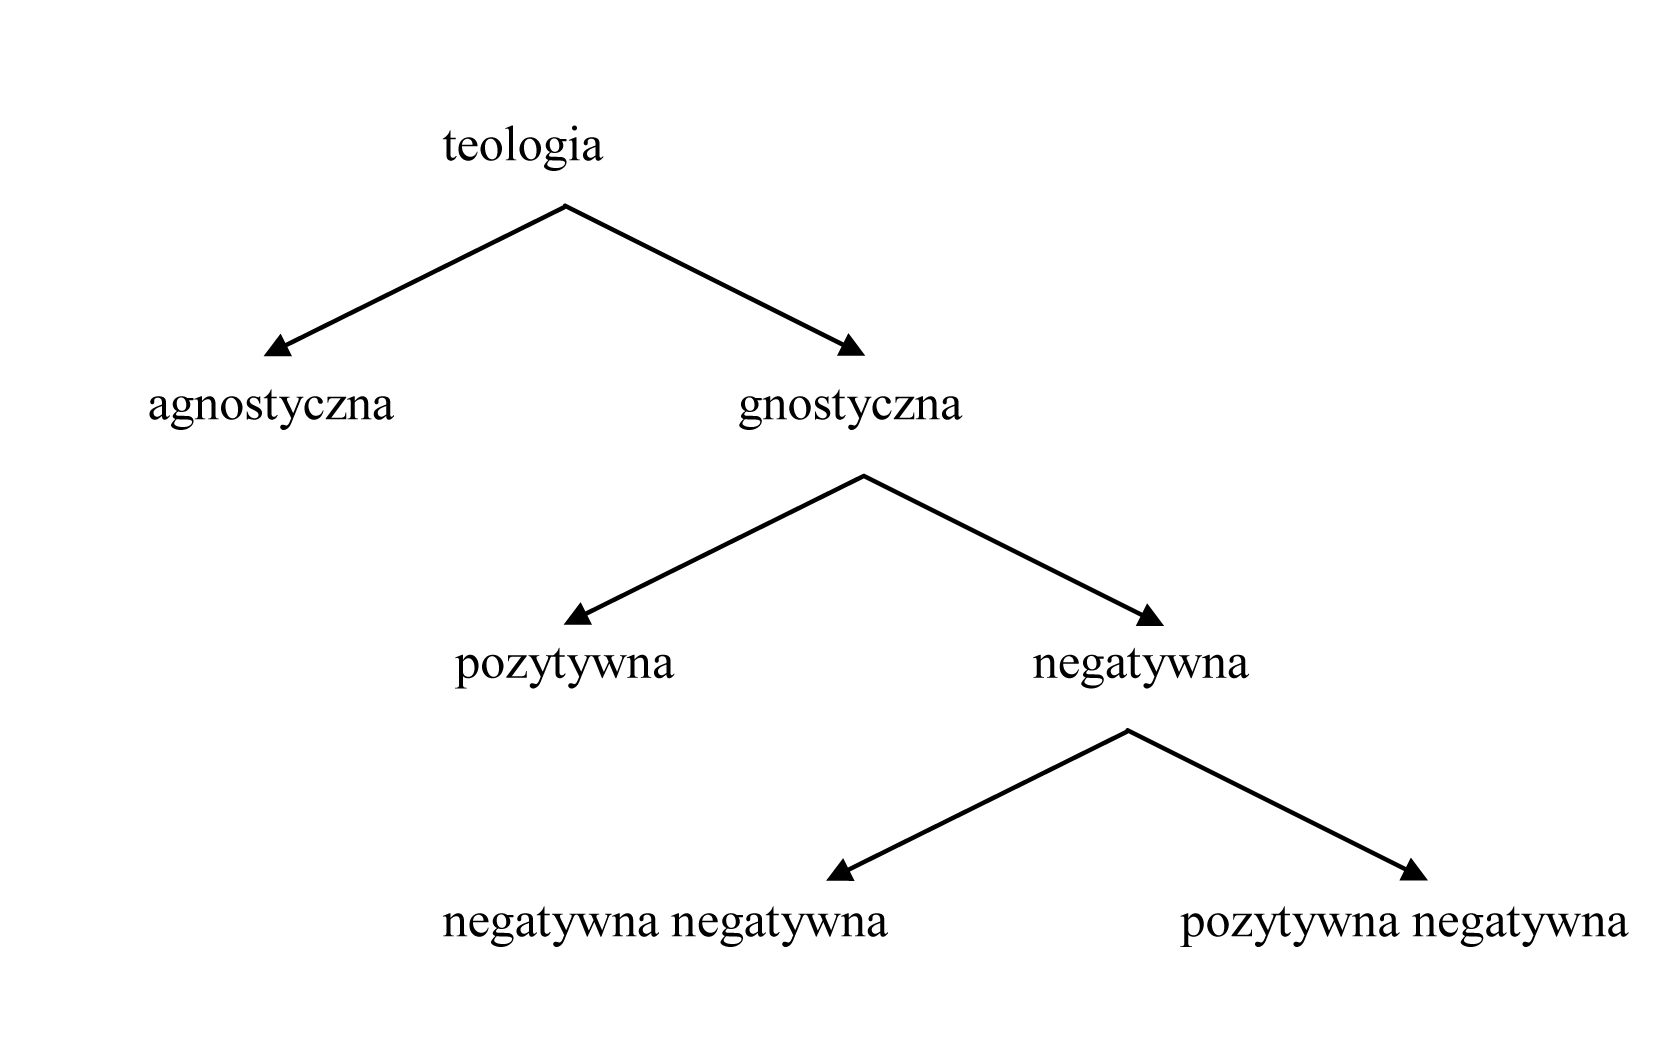
\includegraphics[width=1\linewidth]{typologia.jpg}
\caption{Proponowana przez Rojka
typologia interpretacji teologii apofatycznej.}
}
\end{figure}

Problemem, któremu Rojek poświęca nieco uwagi, lecz mimo wszystko
postanawia go nie rozstrzygać, jest problem własności pozytywnych. Jest
to problem poważny, ponieważ w świetle przedstawionej powyżej typologii
różnica między teologią pozytywną i negatywną polega na orzekaniu o
najwyższej istocie pozytywnych własności lub ich negacji. Jak
zdefiniować zbiór takich własności? Rojek wymienia kryterium
syntaktyczne, które miałoby polegać na „obecności negacji w
predykacie”\footnote{Tamże, s. 221. }. Nie do końca wiadomo, jak
rozumieć takie kryterium. Przypuszczam, że formalnie można zapisać tę
propozycję w logice predykatów II-rzędu w następujący sposób:

\begin{equation}
    P(Q) {=}_{df} \forall x \neg \exists N (Q(x) \equiv \neg N(x)),
\end{equation}
gdzie $P(Q)$ oznacza „własność $Q$ jest pozytywna”. Jednakże Rojek
natychmiast dodaje, że kryterium syntaktyczne nie może być uważane za
wystarczające. Powołuje się tu na klasyczny przykład predykatu „jest
ślepy” -- nie zawiera on negacji, lecz odnosi się do braku i z tego
powodu wydaje się być pozytywny. Trafniejszym argumentem wydaje się być
powołanie na św. Tomasza, wedle którego własności tradycyjnie
przypisywane bytowi absolutnemu, takie jak prostota, doskonałość czy
jedność, są w istocie własnościami negatywnymi\footnote{św. Tomasz z
Akwinu Teologiczna: I, 3, Summa contra Gentiles 11. }.

Problem własności pozytywnych Rojek pozostawia nierozwiązany tłumacząc,
że skupia się na formie teologii negatywnej, nie na jej treści. Dodaje
jednak, że istnieje jeszcze jeden bardzo szczególny sposób ich
rozumienia. Można je traktować, jako najwyższy sposób istnienia danej
własności, czyli tzw. perfekcje. Najczęściej mówi się o takich
perfekcjach, jak wszechwiedza -- najwyższy sposób wiedzy, czy też
wszechmoc -- najwyższy stopień mocy. Są one istotnym elementem w
ontologicznych dowodach istnienia Boga, które w historii były
proponowane m.in. przez św. Anzelma, Kartezjusza, Leibniza, Gödla i
Perzanowskiego. W tych argumentach Boga można uznać za podmiot
wszelkich własności pozytywnych rozumianych jako perfekcje:

\begin{equation}
    G(x) \equiv \forall Q (P(Q) \to Q(x)).
\end{equation}


Definicję tę Rojek zaczerpnął od Perzanowskiego\footnote{J.
Perzanowski, Ontological Arguments II: Cartesian and Leibnizian, [w:]
red. H. Burkhardt, B. Smith, Handbook of Metaphysics and Ontology, t.
2, PhilosophiaVerlag, München 1991,ss.~625–633. } i stanowi ona
wzór kolejnych definicji Boga w proponowanych przez niego następnie
interpretacjach teologii negatywnej. Warto wiec poświęcić jej nieco
uwagi. Po pierwsze, jest ona zapisana w rachunku predykatów drugiego
rzędu, gdyż zawiera warunek, że własności przypisywane Bogu muszą być
pozytywne. Po drugie, Bóg formalizowany jest jako predykat („$x$ jest
Bogiem”, „$x$ jest bogopodobny”), nie jako stała logiczna\footnote{Por.
choćby M. Durrant, The „Meaning of ‘God’-I, Royal Institute of
Philosophy Supplement,vol. 31 (1992), ss. 71-84. }, lub deskrypcja
określona, co proponował Bocheński\footnote{J.M. Bocheński, dz. cyt.,
s. 381. }. Po trzecie, powyższa definicja powstała na użytek
formalizacji dowodów ontologicznych, które należą raczej do jakiejś
formy teologii pozytywnej. Zawarte w niej $P(Q)$ czytamy jako „$Q$ jest
własnością pozytywną” w pewnym szczególnym sensie opisanym powyżej -- „$Q$
jest perfekcją”. Rojek nie sugeruje jednak, że w teologii apofatycznej
Pseudo-Dionizego zaprzecza się jedynie tego typu własnościom
pozytywnym. Przeciwnie, pisze wprost, że zakres negowanych własności
jest szerszy\footnote{P. Rojek, dz. cyt., s. 222. }. Po raz
kolejny jednak odżegnuje się od określenia, o jakie konkretnie
własności chodzi. Jest to, moim zdaniem, jeden z najsłabszych punktów
jego propozycji. Wrócę do tego ponownie w dyskusji.


\subsection{Agnostyczna teologia negatywna}

Strategią pierwszej przedstawianej przez Rojka interpretacji teologii
negatywnej jest przyjęcie (T4) jako tezy podstawowej i odrzucenie lub
modyfikacja pozostałych tez, za cenę zachowania spójności teorii.
Według tej interpretacji, celem teologii negatywnej jest wskazanie
boskiej transcendencji -- głosi ona, że Bóg jest zasadniczo
niepojmowalny i niewyrażalny.

Takie rozumienie teologii negatywnej jest popularne wśród wielu
komentatorów -- także tych, którzy rozważają logiczno-językową strukturę
tej teorii. Wśród nich Rojek wymienia Michaela Gellmana, Johna J.
Jonesa oraz Paula Rorema.

W rozważaniach Gellmana teologia negatywna jest teorią, w której
jakikolwiek predykat P języka „skończonych bytów” nie może być
przedziwie orzekany o Bogu. Jej główną tezą jest, że Bóg nie należy do
zakresu żadnego z predykatów naszego języka. Jeśli mówimy na przykład,
że Bóg nie jest mądry, mamy na myśli raczej negacją
\textit{wykluczającą}, niż negację \textit{wyboru}. Naszym zamiarem
jest wyłącznie stwierdzenie, że to nieprawda, że predykat P przysługuje
Bogu, niekoniecznie sugerując, że można o nim orzec dopełnienie tego
predykatu, czyli nie-P\footnote{J.I. Gellman, The Meta-Philosophy of
Religious Language. „No\^us”, nr 11 (1971), s. 158. }. Według
Gellmana, zdanie „Bóg jest potężny” teolog negatywny zrozumie jako
negację dopełnienia predykatu „jest potężny”. W innym kontekście
oznaczałoby to przypisanie obiektowi, o którym mowa, tej właśnie
własności. Jednakże w przypadku Boga negowanie dopełnienia predykatu P
nie oznacza przypisywania mu P. Mówiąc ogólnie, zdania języka
religijnego negują dopełnienia wszystkich wymienianych przez nie
własności Boga, który jest poza zakresem wszystkich naszych predykatów.
One, z kolei -- będąc predykatami języka skończonych bytów -- z
konieczności muszą oznaczać niedoskonałe własności\footnote{Zob.
Tamże. }.

Według Jonesa, teologia negatywna Pseudo-Dionizego Areopagity jest w
dużej mierze teologią krytyczną. Polemizuje ona z błędnym sposobem
mówienia o Bogu -- takim, który traktuje Go jak byty, czyli rzeczy lub
pojęcia\footnote{J.J. Jones, dz. cyt., s. 357. }. Fakt, że Bóg
przekracza wszelki byt, nadaje również strukturę językowi dyskursu
teologicznego. Nie idzie tylko o to, że przypisywanie Bogu
jakichkolwiek przymiotów przysługujących bytom jest z gruntu błędne.
Zwykle, gdy mówimy o rzeczach, twierdzenia i przeczenia sprzeciwiają
się sobie. W wykładni Dionizego nie dzieje się tak w przypadku Boga.
Bóg nie jest jednym z bytów, zatem język służący do opisu bytów nie
jest dla Niego właściwy. W wypracowanym przez niego języku teologicznym
twierdzenia i zaprzeczenia należą do odmiennych grup, tworząc odmienne
sposoby mówienia o Bogu. Ponieważ funkcjonują one w odmienny sposób,
nie należy ich ze sobą mieszać. Te pierwsze przedstawiają Boga jako
przyczynę wszystkiego, te drugie wyrażają jego transcendencję. Oba
sposoby mówienia można stosować naraz zarówno do opisu Boga, jak i
opisu przedmiotów, jednakże w ten sposób nie zdołamy wyrazić
unikalności Boga -- tego, że jest czymś odrębnym od wszystkich
bytów\footnote{Zob. Tamże, s. 360. }. Możemy tego dokonać
wyłącznie przez negację, która według Jonesa jest kluczowym punktem
myśli Dionizego. Istotnym jest, że Jones wyraźnie odróżnia negację od
zaprzeczenia.


\begin{quote}
        W przeciwieństwie do zaprzeczenia, negacja odnosi się do (nie)możliwości
poznania i powiedzenia czegokolwiek o Bogu. Jest to, jeśli można tak
powiedzieć, reguła drugiego rzędu posługiwania się nazwami pierwszego
rzędu.\footnote{Tamże, s. 381. Większą część tego cytatu podaję za
Rojkiem, dz. cyt., s. 222. }
\end{quote}






Najbardziej agnostyczną interpretację dionizyjskiej teologii negatywnej
zaproponował Paul Rorem. Podkreśla on podobieństwo teologii
Pseudo-Dionizego z późną filozofią neoplatońską. W obu tych doktrynach
byty uporządkowane są względem pewnej hierarchii i w celu dotarcia do
bytu absolutnego należy „wspiąć się” po tej „drabinie” bytów. By
spotkać Boga należy wpierw zanegować nasze wrażenia i wyobrażenia i
przekroczyć je, by dojść do ich pojęciowych znaczeń. Następnie
zanegowane zostać powinny także owe znaczenia oraz wszelkie inne
pojęcia umysłu, ponieważ przekroczenie naszej wiedzy prowadzi do
niepoznawalnego, do cichego zjednoczenia z Bogiem. Innymi słowy, Rorem
zwraca uwagę, że u Areopagity drogą do Boga jest zaprzeczenie
wszystkich bytów. Dionizy jednak wielokrotnie stwierdza, że Bóg jest
także ponad wszelkim zaprzeczeniem. Ostatecznie więc, należy zanegować
także wszelkie negacje, nie pozostawając już żadnym pojęciem
Boga\footnote{Por. P. Rorem, Pseudo-Dionysius. A Commentary on the
Texts and an Introduction to Their Influence, Oxford University Press,
Oxford -- New York 1993, ss. 210-211. }. Jak zauważa Rorem, Dionizy
„zaprzecza i wykracza poza wszystkie nasze pojęcia lub «pojęciowe»
atrybuty Boga i kończy na odrzuceniu wszelkiego mówienia i myślenia,
nawet negatywnego”\footnote{Tenże, przypis do Pseudo-Dionizy
Areopagita, The Complete Work, tłum. C. Luibheid,. Paulist Press, New
York 1987, s. 99. Cytuję za P. Rojek, dz. cyt. }.

Przedstawione powyżej prace pozwalają sądzić, że wynikiem agnostycznej
interpretacji teologii negatywnej nie jest zatem teza, że Bóg posiada
własności negatywne, lecz twierdzenie, że jest On niepoznawalny i
niewyrażalny. Zgodnie ze wskazaną w ten sposób dwuznacznością tezy (T4)
Rojek wyróżnia dwie wersje tej teorii. Wedle pierwszej z nich, Bóg jest
niewyrażalny, nie sposób Go wysłowić. Konsekwentnym rozwinięciem tej
teorii jest stwierdzenie, że dyskurs religijny jest pozbawiony
jakiegokolwiek znaczenia. Wedle drugiej wersji, Bóg jest tylko
niepoznawalny, nie można posiąść o nim wiedzy. I choć dyskurs religijny
posiada w tej teorii jakieś znaczenie, może on opisać wyłącznie to,
czego o Bogu nie wiemy. Rojek omawia obie wersje tej interpretacji.



\subsubsection{Teoria Niewysławialnego}

Według wielu komentatorów ta wersja agnostycznej teologii negatywnej
jest wewnętrznie sprzeczna. Z reguły argumentacja polega na wskazaniu,
że teoria ta twierdząc, że nie da się niczego powiedzieć o Bogu, sama
coś o Nim mówi, a zatem jest sprzeczna. W takim wypadku należałoby ją
odrzucić. Jednym krytyków teorii Niewysławialnego\footnote{Rojek używa terminu „Niewyrażalny”. W
niniejszej pracy pozostaje przy terminologii polskiego przekładu pracy
Bocheńskiego, Logika i teologia, dz. cyt. } jest Michael Durrant.
Pisze on, że

\begin{quote}
    w tej teorii, mówiąc, że natura Boga jest zasadniczo niewyrażalna,
opisujemy właśnie naturę Boga -- jest mianowicie zasadniczo
niewyrażalna. Innymi słowy, ci, którzy bronią tego stanowiska, nie mogą
tego robić nie przecząc sobie.\footnote{M. Durrant, The Meaning of
‘God’ (I). [w:] Religion and Philosophy, red.  M. Warner, Cambridge
University Press, Cambridge 1992, s. 74. Cytuję za P. Rojek, dz. cyt.,
s. 222-223. }
\end{quote}


Podobnie argumentuje John Hick, który uważa, że nie ma sensu


\begin{quote}
mówić o X, że żadne nasze pojęcie się do niego nie stosuje. Jest bowiem
w oczywisty sposób niemożliwe odnosić się do czegoś, co nie posiada
nawet własności 'bycia możliwym przedmiotem
odniesienia.\footnote{J. Hick, An Interpretation of Religion. Human
Responses to the Transcendent, Yale University Press, New Haven –
Londyn 1989, s. 239. Cytuję za P. Sikora, Logos Niepojęty, Wydawnictwo
Universitas, Kraków 2010, s. 118. }
\end{quote}


Dodaje on także, że określenie

\begin{quote}
,,taki, że nasze pojęcia się do niego nie stosują'' nie może,
jeśli chcemy uniknąć paradoksu, odnosić się do własności, którą
opisuje.\footnote{Tamże. }
\end{quote}

Przeciwko takiemu przedstawianiu teorii Niewysławialnego występuje Józef
Maria Bocheński. Twierdzi on, że da się ją uratować od sprzeczności,
lecz nawet mimo tego, nie odpowiada ona potrzebom dyskursu
religijnego\footnote{Zob. J.M. Bocheński, dz. cyt., ss. 353-356.
}. Bocheński uważa, że jeśli przestrzega się pewnych obowiązujących w
logice konwencji, zarzut sprzeczności stawiany teorii Niewysławialnego
przestanie obowiązywać. Należałoby wpierw dowieść, że danym układzie
odniesienia teoria ta prowadzi do sprzeczności, tymczasem nikt takiego
dowodu nie przedstawił. Według Bocheńskiego sytuacja przedstawia się
zupełnie przeciwnie -- nietrudno wykazać, że teoria Niewysławialnego
jest spójna. Poniżej przedstawię jego argumentację.

Załóżmy, że dwuargumentowy predykat  $Nw(x,l)$ oznacza „$x$ jest
niewyrażalne w języku $l$”.

Zapiszmy teraz formułę zawierającą ten predykat

\begin{equation}
    \exists x \exists l Nw(x, l)
\end{equation}


Wydaje się, że nie tylko można ją wypowiedzieć nie popadając w
sprzeczność, lecz także jest ona prawdziwa, nietrudno znaleźć taki
obiekt $x$ i taki język $l$, które spełniałyby zapisany wyżej warunek.
(Bocheński podaje przykład krowy i języka szachów: nie da się opisać
krowy w języku szachów).

Możemy powyższy przykład uogólnić i sformułować metajęzykową definicję
Boga o następującej postaci:

\begin{equation}\tag{G2}
    G(x) \equiv \forall l Nw(x, l)\footnote{Definicję podaję za
Rojkiem, różni się ona od zapisu Bocheńskiego tym, że u tego ostatniego
„Bóg” zapisany został jako stała logiczna: $\forall l Nw(a, l)$.}
\end{equation}



Na pierwszy rzut oka, wydaje się, ze ta formuła jest bardziej
problematyczna -- twierdzenie, że $x$ jest niewysłowione w żadnym języku
zdaje się prowadzić do sprzeczności. Można jednak uniknąć tego
problemu, stosując zwykłe konwencje wykorzystywane do pozbywania się
antynomii semantycznych. Należy założyć, że żadne zdanie traktujące o
pewnej klasie języków, nie jest formułowane w żadnym z tych języków.
Aby było pozbawione sprzeczności musi zostać sformułowane w innym
języku, czyli odpowiednim metajęzyku. Możemy więc założyć, że klasa
języków wspominana w (G2) jest klasą języków przedmiotowych. W takim
wypadku (G2) jest zdaniem metajęzyka pierwszego stopnia. Po takim
zabiegu, sformułowana definicja jest znacząca i pozbawiona
sprzeczności. Nie ma bowiem niespójności w twierdzeniu, że coś nie daje
się wysłowić w jakimś języku, lub nawet w klasie języków, o ile
twierdzenie to jest w języku nienależącym do tej klasy. Według
Bocheńskiego, przy takim założeniu, standardowym z punktu widzenia
logiki ogólnej, teoria Niewysławialnego pozostaje znacząca i spójna a
zarzut sprzeczności zostaje oddalony.

Bocheński odrzuca jednak teorię Niewysławialnego z co najmniej dwóch
powodów. Po pierwsze, na mocy (G2) nie można przypisać Bogu
jakiekolwiek własności językowo przedmiotowej. Jedyną własnością, jaką
możemy mu przypisać, jest metajęzykowa własność bycia niewysłowionym w
żadnym z języków przedmiotowych. W takim wypadku wierny, nie mógłby
akceptować żadnego zdania dyskursu religijnego, które przypisałoby Bogu
jakąkolwiek własność-przedmiotowo-językową. Wydaje się to niespójne z
faktycznym dyskursem religijnym. Po drugie, niemożliwe byłoby oddawanie
czci obiektowi, o którym wiemy tylko i wyłącznie, że nie można o nim
nic powiedzieć. Jeśli wierny miałby czcić obiekt pozbawiony własności
przedmiotowo-językowych, równie dobrze tym obiektem mógłby nie być Bóg
a szatan\footnote{Por. J.M. Bocheński, dz. cyt., ss. 354-356. }.

Rojek dodaje do tego podobny argument, jednakże umieszczony w kontekście
teologii negatywnej. Mianowicie, jeśli teoria Niewysławialnego ma być
właściwą interpretacją teologii negatywnej, można poddać w wątpliwość
zasadność jednoczesnego utrzymywania tez (T1)-(T3). Jeśli Bóg jest
niewyrażalny, cały język religijny jest pozbawiony znaczenia, nie
możemy więc ani sensownie potwierdzić, ani zaprzeczyć żadnym z Jego
własności. Dla Rojka jest to wskazówka, by (T4) nie interpretować
semantycznie, lecz epistemologicznie lub nawet ontologicznie\footnote{
Zob. P. Rojek, dz. cyt., s. 223. }. W ten sposób przechodzi się od
teorii Niewysławialnego do teorii Niepoznawalnego.


\subsubsection{Teoria Niepoznawalnego}

Teoria Niepoznawalnego jest lepszym modelem teologii apofatycznej,
ponieważ nie tylko przyjmuje (T4) za twierdzenie podstawowe, lecz także
umożliwia pewną interpretację tez (T2) oraz (T3).By to pokazać, Rojek
wprowadza pojęcie nieokreśloności oraz definiuje nowe, odmienne od
klasycznego pojęcie negacji. W tym celu wykorzystuje on logiczną teorię
nieokreśloności, którą na potrzeby modelowania filozofii nauki rozwinął
rosyjski logik, Aleksander Zinowjew\footnote{A. Zinowjew, Foundations
of the Logical Theory of Scientific Knowledge (Complex Logic), D.
Reidel Publishing Company, Dordrecht 1967. Zob. Także A. Zinowjew,
Logika nauki, tłum. Z. Simbierowicz, PWN, Warszawa 1976. }.

Zinowjew rozważa pewne nieklasyczne przypadki, do których nie można
zastosować prawa wyłączonego środka. Polegają one na przyjęciu
możliwości istnienia obiektów, co do których nie da się ustalić, czy
posiadają one jakąś własność $Q$, czy też posiadają własność
$\neg Q$. Takimi obiektami mogą być na przykład rozważana
w mechanice kwantowej cząstka elementarna, której parametry -- zgodnie z
zasadą nieoznaczoności -- nie mogą zostać ustalone, twierdzenie, które
na gruncie danego rachunku logicznego nie może zostać ani dowiedzione,
ani obalone, albo po prostu obiekt zmieniający się w czasie. Na
potrzeby tych przypadków wprowadźmy nowy funktor nieokreśloności i
oznaczmy go $?$\footnote{Dla utrzymania spójności zapisu, formuły teorii
nieokreśloności Zinowjewa przedstawiam w notacji zaproponowanej przez
Rojka, dz. cyt., s. 223.  }. Niech zapis $?Q(x)$ oznacza „nie można
ustalić, czy $Q(x)$, czy $\neg Q(x)$”, to znaczy „$x$ ma w sposób
nieokreślony $Q$”. Ponieważ w teorii Niepoznawalnego Bóg uznawany jest za
obiekt, którego nie da się poznać, za pomocą powyższego funktora możemy
podać nową definicję Boga, jako obiektu, który wszystkie swoje
własności posiada w sposób nieokreślony.

\begin{equation}\tag{G3}
   G(x) \equiv \forall Q (P(Q) \to ?Q(x)).
\end{equation}



Formule tej należy poświęcić nieco uwagi. Po pierwsze, w odróżnieniu od
(G2) powyższa definicja nie jest wyrażona w metajęzyku, lecz w języku
przedmiotowym. Po drugie, co istotniejsze, by uniknąć kłopotów z
formalizowaniem Boga przy użyciu predykatu $G(x)$, należy ją ograniczyć.
Do tej definicji trzeba dołożyć dodatkowe założenie, o postaci:

\begin{equation}
    \neg P(G)
\end{equation}


Innymi słowy, należy założyć, że predykat „jest Bogiem” (lub „jest
bogopodobny”) nie należy do zbioru predykatów pozytywnych. W
przedziwnym bowiem razie, wpadlibyśmy w błędne koło i o niczym nie
można byłoby określić, że jest Bogiem.

Jak zauważa Rojek, wykorzystując ten formalizm do modelowania teorii
Niepoznawalnego, można -- w pewnym szczególnym sensie -- zaprzeczyć, że
Bóg posiada wszystkie własności pozytywne. Oczywiście, nie idzie tutaj
o stwierdzenie, że o Bogu można na orzec jakiekolwiek
$\neg Q$, przy założeniu, że $Q$ jest własnością pozytywną.
Taki przypadek jest niezgodny definicją (G3). Idzie o to, że po
wprowadzeniu funktora nieokreśloności $?$, zdanie „nieprawda, że $x$ jest
$Q$”\footnote{Rojek mówi o wyrażeniu „$x$ jest nie-$Q$”, moim zdaniem
błędnie. Por. tamże. } staje się dwuznaczne. Może ono przyjąć jedno
z dwóch znaczeń: albo „$x$ jest nie-$Q$”, albo „nie można stwierdzić, czy $x$
jest $Q$”. W nomenklaturze Rojka, w pierwszym przypadku z zdaniu pojawia
się negacja w znaczeniu \textit{de re}, o drugim znaczeniu natomiast
można mówić, że zawiera ono negację \textit{de dicto}. Nieco inne
nazewnictwo wprowadził Zinowjew, który pierwszy rodzaj negacji nazwał
negacją wewnętrzną -- dotyczy ona bowiem wyłącznie predykatu, drugi
negacją zewnętrzną -- odnosi się ona bowiem do całego negowanego w ten
specyficzny sposób zdania.

Przyjmijmy teraz dwa różne symbole, w celu odróżnienia odmiennych pojęć
negacji. Niech $\neg$ oznacza negację \textit{de re},
natomiast symbol $\sim$ negację \textit{de dicto}. Przy
takiej notacji, formułę $\neg Q(x)$ czytamy jako „$x$ jest
nie-$Q$”, lub  inaczej: „$x$ ma własność nie-$Q$”\footnote{U Rojka: „$x$ ma
własność $\neg Q$”. }, natomiast formuła
$\sim\! Q(x)$\footnote{Rojek formułę, negowaną za pomocą
funktora $\sim$ opatruje w dodatkowe nawiasy po to, by
podkreślić odmienny, „zewnętrzny” charakter tego rodzaju negacji.
Uznaję ten zabieg za niekonieczny. Notacja Rojka jest odmienna od
stosowanej oryginalnie przez Zinowjewa. } oznacza „nie można
stwierdzić, czy $x$ jest $Q$”, lub  innymi słowy „nie jest twierdzi się, że
$x$ ma własność $Q$”. Poniższe aksjomaty definiują relacje, jakie zachodzą
pomiędzy funktorem nieokreśloności a funktorami negacji \textit{de re}
oraz negacji \textit{de dicto}:

\begin{equation}\tag{Z1}
\sim\! Q(x) \equiv ?Q(x) \lor \neg Q(x),
\end{equation}
\begin{equation}\tag{Z2}
\sim\!\neg Q(x) \equiv Q(x)\ \lor\ ?Q(x),
\end{equation}
\begin{equation}\tag{Z3}
\sim ?Q(x) \equiv Q(x) \lor \neg Q(x).
\end{equation}
Na ich podstawie można dowieść następujących tez:

\begin{equation}
   \vdash \quad ?Q(x)\ \equiv\ \sim\! Q(x)\ \land\ \sim\!\neg Q(x).
\end{equation}
 



Gdybyśmy chcieli dokonać kolapsu z powrotem do logiki klasycznej,
musielibyśmy przyjąć założenie, że negacje \textit{de re} i \textit{de
dicto} są wzajemnie definiowalne, to znaczy, że
$\neg Q(x) \equiv \sim\!Q(x)$. Jednakże, jeśli
chcemy opisać wspomniane wyżej przypadki nieklasyczne, w których
posiadanie lub nie posiadanie danej własności przez konkretny obiekt
nie może zostać określone, musimy zgodzić się na posiadanie dwóch
różnych, nierównoważnych pojęć negacji w systemie. Z tego powodu
poniższa formuła nie jest tezą prezentowanego rachunku:


\begin{equation}
    \nvdash \quad \sim\! Q(x) \to  \neg Q(x).
\end{equation}
Dzieje się tak, ponieważ $\sim\!Q(x)$ pociąga za sobą $\neg Q(x)$ lub
$?Q(x)$. Analogicznie, w prezentowanym tu rachunku nie zachodzi
następująca wersja prawa podwójnej negacji



\begin{equation}
   \nvdash \quad  \sim\! (\neg Q(\textit{x})) \to  Q(\textit{x}),
\end{equation}
ponieważ $\sim\!\neg Q(x)$ implikuje $Q(x)$ lub $?Q(x)$. Prawdziwe są
natomiast następujące formuły:



\begin{equation}
    \vdash \quad \neg Q(x) \to  \sim\! Q(x),
\end{equation}
\begin{equation}
    \vdash \quad Q(x) \to  \sim\! \neg Q(x).
\end{equation}






Należy zauważyć, że w przypadka z nieokreślonością nie można także mówić
o klasycznym prawie wyłączonego środka


\begin{equation}
     \nvdash \quad Q(x) \lor \neg Q(x),
\end{equation}
ponieważ istnieje dodatkowa, trzecia możliwość - $?Q(x)$. Do grona tez tego
rachunku należy zatem następująca formuła:

\begin{equation}
    \vdash \quad Q(x) \lor  \neg Q(x) \lor  ?Q(x)
\end{equation}


Co ciekawe, prawo wyłączonego środka obowiązuje dla negacji \textit{de
dicto}:

\begin{equation}
    \vdash \quad Q(x) \lor  \sim\! Q(x),
\end{equation}
\begin{equation}
    \vdash \quad \neg Q(x) \lor  \sim\! \neg Q(x),
\end{equation}
\begin{equation}
\vdash \quad ?Q(x) \lor  \sim\! ?Q(x).
\end{equation}

Jak zauważył Rojek, rachunek Zinowjewa stworzony pierwotnie na potrzeby
formalizacji teorii naukowych jest przydatny także do modelowania
omawianej w tym paragrafie interpretacji teologii apofatycznej. Dzięki
jego własnościom, można przedstawić w nim w sposób niesprzeczny aż trzy
tezy wypreparowane z pism Pseudo-Dionizego Areopagity. Formalną wersją
tezy (T4) jest definicja Boga podana przez (G3). Negację, o której mowa
w (T2) można traktować, jako negację \textit{de dicto}, ponieważ
zgodnie z teorią niepoznawalności Boga, nie możemy stwierdzić, czy
posiada On jakieś własności. W takim podejściu, (T2) stwierdza, że o
Bogu można orzec zewnętrzne negacje wszystkich własności pozytywnych. A
zatem, w języku tego rachunku należałoby to zapisać w następujący sposób:



\begin{equation}
    G(x) \to  (\forall Q (P(Q) \to  \sim\!Q(x)).
\end{equation}



Co więcej, powyższa formuła jest bezpośrednią konsekwencją definicji
(G3) i (1), które jest jednym z praw tego rachunku. Ponieważ negacja
\textit{de dicto}, jest różna od negacji \textit{de re}, nie możemy
jednocześnie twierdzić, że Bóg posiada (wewnętrzną) negację wszystkich
pozytywnych własności, czyli, że można o nim orzekać każde nie-$Q$, o ile
$Q$ jest pozytywne. Dzieje się tak, ponieważ z obu tych formuł wynika
także


\begin{equation}
    G(x) \to  (\forall Q (P(Q) \to
\sim\!\neg Q(x)),
\end{equation}


którą Rojek uważa za formalną postać tezy (T3). Formuła ta zawiera
podwójne przeczenie, jednakże pierwsza negacja ma charakter \textit{de
dicto}, natomiast druga jest negacją \textit{de re}. Brzmieniem tej
formuły jest „Nie można stwierdzić, czy Bóg posiada wszystkie negacje
pozytywnych własności”.

W takim wypadku, wszystkie stwierdzenia Dionizego o tym, że Bóg nie jest
ani $Q$, ani nie-$Q$, na przykład że nie jest On „ani wielkością, ani
małością, ani równością, ani nierównością, ani podobieństwem, ani
niepodobieństwem”, „nie jest też niczym z niebytu ani czymś z
bytu”\footnote{Pseudo-Dionizy Areopagita, Teologia mistyczna, dz.
cyt., rozdział V. } itp.,  można z łatwością interpretować w
świetle powyższej formalizacji. Podobnie sformułowania Areopagity o
tym, że Bóg jest „ponad wszelkim twierdzeniem i ponad wszelkim
zaprzeczeniem”\footnote{Tamże. } można ująć w ramach
prezentowanego rachunku, jako koniunkcję warunków zawartych już w
formułach (8) i (9).


\begin{equation}
    G(x) \to  (\forall Q (P(Q) \to  \sim\!(Q(x)) \land
\sim\!\neg Q(x)).
\end{equation}



Jak zauważa Rojek, istnieje wyjątek od konsekwentnego stosowania tej
interpretacji. Nie można w ten sposób formalizować  twierdzeń, że Bóg
nie jest ani poznawalny ani niepoznawalny, ani określony, ani
nieokreślony. Taka treść predykatu $Q$ naraziłaby bowiem tę interpretację
na sprzeczność. Jednakże wydaje się, że żadne z dzieł Dionizego nie
zawiera podobnych sformułowań\footnote{Także Jones zauważa, że teza o
niepoznawalności Boga ma wyjątkowy charakter w pismach Dionizego i
nigdy nie występuje w podobnych parach. Zob. J.J. Jones, dz. cyt., s.
358. }. Jedynie (T1) nie znajduje swojego miejsca w powyższej
interpretacji, bowiem -- skoro Bóg jest niepoznawalny -- nie można o nim
nic sensownie stwierdzić.

Powyższe analizy pozwalają sądzić, że wykorzystując odpowiednie
narzędzia formalne można obronić przed sprzecznościami obie formy
agnostycznej teologii negatywnej -- zarówno teorię Niewysławialnego, jak
i teorię Niepoznawalnego. Ta druga wydaje się o tyle lepszą
interpretacją teologii Pseudo-Dionizego, o ile na jej gruncie można
przyjąć aż trzy z wypreparowanych z tekstu Areopagity tez. Teoria
Niewysławialnego ustępuje w tym zestawieniu  i obejmuje tylko jedną
tezę dionizyjskiej doktryny. Obie jednak zawodzą w interpretacji (T1) i
jak zauważył Bocheński -- są zasadniczo niespójne z faktycznym dyskursem
i praktyką religijną. Zgodnie z ich duchem, wierny nie mógłby
akceptować żadnych zdań dyskursu religijnego, które przypisują Bogu
jakieś własności. Tymczasem, każdy dyskurs religijny zawiera
przynajmniej kilka takich zdań. Poza tym, gdyby o Bogu nie można było
orzekać żadnych własności, nie mógłby On być przedmiotem czci\footnote{
Zob. J.M. Bocheński, dz. cyt., ss. 355-356.}.




\subsection{Negatywna teologia negatywna}

Wad tych pozbawiona jest druga interpretacja teologii negatywnej, którą
Rojek nazywa negatywną teologią negatywną. Jej punktem wyjścia jest
teza (T2). Na gruncie tej interpretacji nie twierdzi się ani, że
dyskurs religijny pozbawiony jest znaczenia, ani że Bóg jest
niepoznawalny. Uważa się natomiast, że o przedmiocie religijnym można
orzekać wyłącznie negatywne własności. Nie jest więc tak, że nic nie
wiemy o Bogu -- wiemy, że nie posiada on pozytywnych własności. Należy
przyznać, że jest to dość popularna interpretacja teologii
apofatycznej. Na przykład, do właśnie w taki sposób rozumianej teologii
negatywnej odnosił się Józef Maria Bocheński w dziele \textit{Logika
religii}.

W analizie Rojka, negację obecną w (T2) na gruncie tej interpretacji
należy traktować jako zwykłą, klasyczną negację. Jeśli przyjmiemy
logikę klasyczną, zachowujemy zasadę niesprzeczności. W konsekwencji,
tezy (T1) oraz (T3) muszą zostać odrzucone, jako niespójne z tezą
przyjętą tu za podstawową.

Wedle tej wersji teologii negatywnej, wszystko, co możemy orzec o Bogu,
posiada ściśle negatywny charakter. Na tym polega boska transcendencja.
Choć Bóg zatraca tutaj swój sprzeczny charakter (obecny w jakimś
stopniu w agnostycznej teologii negatywnej), wciąż pozostaje w jakimś
sensie niepoznawalny. Jedyne, co o Nim wiemy to jaki nie jest. Można
więc pokusić się także na próbę uwzględnienia tezy (T4) w obrębie
niniejszych analiz.

Rojek twierdzi, że w tym modelu teologii negatywnej właściwą definicją
Boga jest formalizacja tezy (T2) w obrębie klasycznego rachunku
predykatów II-rzędu. Bóg -- analogicznie do poprzednich definicji –
opisany jest jako obiekt, o którym można orzekać negacje wszystkich
pozytywnych własności:


\begin{equation}\label{G4}\tag{G4}
    G(x) \equiv  \forall Q (P(Q) \to
\neg Q(x)).
\end{equation}





Podobnie, jak poprzednie definicje, także formuła (G4), wymaga
wprowadzenia szeregu ograniczeń po to, by w proponowany model nie
wkradła się żadna sprzeczność. Pierwsze ograniczenia dotyczą zbioru
pozytywnych własności. Jak wspominałem wcześniej, Rojek nie podaje
żadnej definicji, ani kryterium wyróżniania własności pozytywnych ze
zbioru wszystkich własności. Czyni jednak na ten temat kilka uwag,
które w większym bądź mniejszym stopniu nawiązują do rozważań
Bocheńskiego

Po pierwsze, według Rojka, zbiór pozytywnych własności nie może zawierać
własności negatywnych. Szczerze powiedziawszy, nie jest do końca jasne
także to, jak Rojek rozumie pojęcie własności negatywnej. W tym wypadku
jednak mamy dość tradycyjną, syntaktyczną definicję tego pojęcia.
Własność negatywna, zwana czasem także własnością dopełniającą, jest
jedną z własności złożonych i stanowi po prostu negację własności. W
języku naturalnym pojęcie negacji własności wrażamy prze użycie
przedrostka \textit{nie}- (w języku łacińskim
\textit{non}-)\footnote{Zob. J. Paśniczek, Predykacja, Copernicus
Center Press, Kraków 2014. }. Wydaje się, że Rojek pojęcie
własności negatywnej rozumie w podobny sposób, twierdzi bowiem, że nie
stosując tego ograniczenia, doprowadzimy do orzekania o Bogu także
własności pozytywnych (co z kolei sugeruje, że jest on także bliski
stosowaniu syntaktycznej definicji własności pozytywnej -- jako
niezawierającej spójnika negacji). Według Rojka, jeśli nie wprowadzimy
tego ograniczenia, nasz model umożliwi pozytywne twierdzenia o Bogu,
bowiem w przyjętej tu logice klasycznej $\neg \neg Q$
implikuje $Q$. Ponadto uważa on, że dopuszczenie do
zaprzeczania własności negatywnych wprowadzi do systemu sprzeczność,
bowiem umożliwi orzekanie o Bogu zarówno $\neg Q$, jak i
$\neg \neg Q$\footnote{Myślę, że
konsekwencji tej można by uniknąć wprowadzając porządną definicję
własności pozytywnych. Niestety, jak już zostało wspomniane, nie
została ona podana. }. Jednakże dla Rojka syntaktyczne kryterium
wyróżniania własności pozytywnych nie jest satysfakcjonujące.
Alternatywą dla niego byłoby kryterium epistemologiczne, zaproponowane
przez Bocheńskiego\footnote{J.M. Bocheński, dz. cyt., s. 416. }.
Wedle tego kryterium własności pozytywne definiuje się indukcyjnie,
jako własności postrzegane bezpośrednio lub zapisywane za pomocą
formuł, zawierających wyłącznie symbole własności pozytywnych i terminy
logiki pozytywnej. Rojek zgadza się z Bocheńskim, że także takie
kryterium nie jest wystarczająco ścisłe. Nie zamierza jednak
rozwiązywać tego problemu i podawać odpowiedniej definicji\footnote{
Por. P. Rojek, dz. cyt., s. 226. }.

Po drugie, po raz kolejny należy wykluczyć predykat „jest Bogiem” ze
zbioru predykatów oznaczających własności pozytywne. Uznanie własności
bycia Bogiem za własność pozytywną doprowadziłoby do sprzeczności:

\begin{equation}
    G(x) \equiv \neg G(x).
\end{equation}


Wedle Rojka, twierdzenie „Bóg nie jest boski” należy przeinterpretować w
taki sposób, by w orzeczniku tego zdania nie znalazł się predykat $G(x)$,
który użyty jest w (G4), lecz wiązka pozytywnych własności zwykle
przypisywanych Bogu. W mojej opinii problem ten mógłby zostać
rozwiązany poprzez formalizowanie Boga przy pomocy stałej logicznej,
zamiast predykatu „$x$ jest Bogiem”.

Jeśli przyjmiemy wszystkie te ograniczenia na proponowaną powyżej
definicję Boga, możemy doprowadzić ten model do ciekawych filozoficznie
konsekwencji. Zgodnie z omawianą wcześniej interpretacją Johna J.
Jonesa, głównym celem Dionizego było wykazanie, że Bóg jest ponad
wszelkim bytem, w szczególności nie należy on do kategorii przedmiotów.
Według popularnego rozumienia przedmiotu, można traktować go jako
podmiot własności. Taką definicją posługiwał się na przykład Stanisław
Leśniewki, według którego coś jest przedmiotem, o ile istnieje jakaś
własność, którą można o nim orzec\footnote{Rojek powołuje się tu na
dwa źródła: J. Słupecki, Stanisław Leśniewski’s Calculus of Names,
„Studia Logica”, nr 3 (1955), ss. 7--76 oraz J. Perzanowski, The Way
of Truth, [w:] red. R. Poli, P. Simons, Formal Ontology, Kluwer
Academic Publishers, Dordrecht 1996, ss. 61--130. }:

\begin{equation}
    Ob(x) \equiv  \exists Q  (Q(x)).
\end{equation}


Jeśli uzupełnimy tę definicję o warunek, że każdy przedmiot powinien
posiadać nie jakąkolwiek, ale pozytywną wartość, otrzymamy następującą
modyfikację\footnote{W świetle stawianych na definicję (G4) ograniczeń
konieczność wprowadzania w tę definicję dodatkowego zastrzeżenia wydaje
się wątpliwa. }:

\begin{equation}\label{D4}\tag{D4}
    Ob(x) \equiv  \exists Q P(Q) \land  Q(x).
\end{equation}


Zgodnie z tak zmodyfikowaną definicję, Bóg nie należy do zbioru
przedmiotów, ponieważ nie może on posiadać żadnych pozytywnych
własności.

\begin{equation}
    \forall x (G(x) \to  \neg Ob(x))\footnote{U Rojka zmienna x nie jest związana
    żadnym kwantyfikatorem}.
\end{equation}


Rojek konkluduje, ze gdy przyjmiemy powyższe rozważania za dobrą monetę,
Bóg istnieje w jakiś inny sposób, odmienny od tego, jak istnieją inne
byty. Według niego można tu mówić o istnieniu w sensie Quine’a (w
przeciwieństwie do istnienia w sensie przedmiotów Leśniewskiego).
Konkluzja ta zdaje się być w zgodzie z  rozważaniami tych zwolenników
teologii negatywnej, którzy podkreślają transcendencję Boga -- to, że
przekracza on wszystkie byty. W przedstawianym powyżej modelu nie można
Go bowiem traktować jako przedmiot w sensie uchwyconym w definicji
(D4).

Czy Bóg zdefiniowany za pomocą (G4) jest poznawalny? W jakimś sensie
możemy wyrazić jego naturę -- możemy mówić, jaki nie jest. Jednakże,
uczciwie rzecz ujmując, na gruncie tego modelu  nie możemy posiąść
żadnej pozytywnej wiedzy o Bogu. Z tego powodu w tej teorii znajdzie
się również miejsce na pewną interpretację tezy (T4). Rojek ujmuje ją w
następujący sposób:



\begin{quote}
    W normalnym wypadku rozumiemy natury rzeczy przez porównanie ich z tym,
czym one nie są. Jak mawiał Spinoza, „określenie jest negacją”. Bez
opozycji znaczeniowych i różnic nie moglibyśmy używać języka w sposób,
w jaki go faktycznie używamy. Bóg jako negacją wszelkich własności
znajduje się jednak poza całym systemem opozycji i różnic. Pełna
negacja prowadzi do całkowitego nieokreślenia.\footnote{P. Rojek, dz.
cyt., s. 226. }
\end{quote}




A zatem w pewnym sensie także na gruncie tej teorii możemy mówić o
niepoznawalności czy nawet niewyrażalności Boga.

Przedstawiony powyżej model teologii negatywnej -- o ile zgodzimy się na
wszystkie jego ograniczenia -- można uznać za logicznie spójny. Choć nie
uwzględnia on wszystkich tez wyabstrahowanych z dzieła Areopagity, w
atrakcyjny sposób rozwija on tezę o wyłącznie negatywnym charakterze
wiedzy o Bogu. Ponadto, nie wymaga on stosowania wyrafinowanych
narzędzi formalnych, pozostając przy logice klasycznej. Jego dodatkowym
atutem jest pewna interesująca filozoficznie własność -- Bóg rozumiany
jest tu jako istotnie odmienny od całej dziedziny bytów rozumianych
jako przedmioty. Jednakże w prezentowanym modelu nie ma miejsca na
interpretację tez (T1) oraz (T3). Ponadto, trudno go pogodzić z
dyskursem i praktyką religijną -- trudno jest bowiem oddawać cześć
czemuś, o czym wiemy tylko, czym nie jest\footnote{Jest to zarzut
stawiany przez Bocheńskiego, dz. cyt., s. 418. }.



\subsection{Pozytywna teologia negatywna}

Ostatnia interpretacja teologii negatywnej jest autorskim pomysłem
Rojka\footnote{Por. P. Rojek, dz. cyt., ss. 227-230. }. Również na
jej gruncie, podstawą tezą teologii negatywnej jest (T2). A zatem o
Bogu można orzec wyłącznie własności negatywne. Ponieważ model
stosowany do formalizacji tej interpretacji używa pewnego
specyficznego, nieklasycznego pojęcia negacji (innego niż wprowadzona
we wcześniejszych rozdziałach negacja \textit{de divto}), może on
również zinterpretować w odpowiedni sposób także tezy (T2) oraz (T3).
Model ten może również zawrzeć satysfakcjonującą interpretację tezy
(T4).

Punktem wyjścia interpretacji Rojka jest spostrzeżenie, że negacje w
pojawiające się tezxach teologii negatywnej Pseudo-Dionizego pełnią
specyficzną funkcję, odmienną od funkcji negacji klasycznej. Dionizy
zdawał sobie sprawę, że negacje, które stosuje nie należy rozumieć w
sensie braku (\textit{privatio}). Twierdził też, że w przypadku
wypowiedzi o Bogu „nie należy sądzić, że zaprzeczenia i twierdzenia
sprzeciwiają się sobie”\footnote{Pseudo-Dionizy Areopagita, dz. cyt.,
rozdział I, 2. }. Uznawał on więc możliwość jednoczesnego przyjęcia
zarazem twierdzenia o Bogu, jak i zaprzeczenie tego twierdzenia. Jak
zauważa Rojek, Dionizy wielokrotnie powtarza, że Bóg jest „powyżej”,
„poza” i „ponad” bytami lub że je „obejmuje”. Poniższy cytat jest
przykładem tego, jak Dionizy używał negacji:



\begin{quote}
    [Bóg] jest wszystkim jako przyczyna wszystkiego […]. I jest ponad
wszystkim, istniejąc ponadsubstancjalnie wcześniej niż wszystko, co
jest. Dlatego też wszystko na raz można o Nim twierdzić, choć On nie
jest żadną rzeczą.\footnote{Tamże, rozdział V, 8. }
\end{quote}





W obliczu takich sformułowań Rojek stwierdza, że dionizyjska negacja
oznacza jednoczesne zawieranie czegoś oraz byciu poza czy też ponad to
coś. W takim rozumieniu, negacja używana przez Areopagitę nie wyklucza
afirmacji. Rojek dodaje, że nawet jeśli tak rozumiane przeczenie nie
powinno się nazywać negacją, to zarzut stawiany Dionizemu nie powinien
polegać na oskarżaniu go o sprzeczność, tylko o niewłaściwe użycie
słów.

Rojek próbuje wykazać, że podobne rozumienie negacji można spotkać także
w języku potocznym. W tym celu posługuje się następującym przykładem:

\begin{quote}
    Załóżmy, że na stole leży 100 tysięcy zł w gotówce (nie jest to łatwe w
trakcie kryzysu). Załóżmy dalej, że ktoś pyta, czy na stole jest 10
groszy. Odpowiedź twierdząca byłaby oczywiście słuszna, lecz w pewien
sposób myląca. Wydaje się, że odpowiedź przecząca byłaby dopuszczalna,
a nawet bardziej wskazana. „Nie, ponieważ na stole leży o wiele, wiele
więcej niż 10 groszy”. Słowo „nie” nie oznacza w tej odpowiedzi
klasycznej negacji, lecz wyraża nieadekwatność supozycji pytania do
zachodzącego stanu rzeczy. Odpowiedź „tak” na to pytanie sugerowałaby,
że suma na stole jest w jakiś sposób porównywalna z 10 groszami. Taka
sama sytuacja zachodzi w wypadku takich pytań jak: „Czy Jan jest
zwierzęciem” („Nie! Jest człowiekiem!”), „Czy Romeo lubi Julię?” („Nie!
On ją kocha!”) itd.\footnote{P. Rojek, dz. cyt., s. 227. }
\end{quote}






Można mnożyć analogiczne przykłady. W podobnym duchu można stwierdzić,
że na obiedzie u teściowej na pytanie „Czy zupa była dobra?” dużo
lepiej (i bezpieczniej) jest odpowiedzieć „Nie, była pyszna!”.
Przykłady te wskazują, że w pewnych wypowiedziach  języka naturalnego
używamy zaprzeczeń, które polegają na klasycznej negacji logicznej. Jak
zauważa Rojek, przeczenie to ma również pozytywny, nie tylko negatywny
charakter i wyraża nie brak, ale nadmiar. Ponadto, uważa on, że takie
użycie przeczenie nie narusza reguł konwersacyjnych Grice’a, w
szczególności reguły ilości, która zabrania przekazywania większej
ilości informacji niż jest to konieczne. Informacja o tym, że dany
obiekt jest czymś większym, niż sądzi rozmówca, w pewnych kontekstach
wydaje się niezbędna. Nawet gdyby reguła ilości została naruszona,
zarzut ten jest dużo słabszy od zarzutu popadania w
sprzeczność\footnote{Zob. tamże. }.

W celu uzasadnienia stosowności używania tego rodzaju „pozytywnej”
negacji Rojek podaje też jego przykłady z dyskursu filozoficznego.
Podobne rozumienie negacji można spotkać u Stróżewskiego, który
rozróżnia dwa rodzaje negacji: przekreślający oraz różnicujący. Ta
pierwsza usuwa negowaną rzecz, ta druga jedynie podkreśla różnicę i jej
rezultatem nie jest brak, lecz w zasadzie jakieś pozytywne
stwierdzenie\footnote{Por. W. Stróżewski, Z problematyki negacji, [w:]
Tenże, Istnienie i sens, Wydawnictw Znak, Kraków 1994,
s.~373--395. }. Podobnego sensu negacji Rojek doszukuje się także
w heglowskim terminie \textit{Aufhebung}, które zwykle tłumaczy się
jako negację lub zniesienie. Powołuje się on na cytat z Hegla, który
wskazuje na dwuznaczny charakter tego słowa:

\begin{quote}
    Należy pamiętać o podwójnym sensie niemieckiego słowa aufheben
(odkładać, ściągać). Aufheben znaczy, po pierwsze, usuwać, anulować,
stąd mówi się, że prawo czy instytucja zostały anulowane. Po drugie,
aufheben znaczy także zachować, i w tym sensie mówimy, że coś zostało
zachowane. Tego podwójnego użycia języka, który nadaje temu samemu
słowu znaczenie pozytywne i negatywne, nie należy traktować jako czegoś
przypadkowego, ani tym bardziej krytykować język za wywoływanie
zamieszania. Powinniśmy raczej dostrzec w tym spekulatywnego ducha
naszego języka, przekraczającego podziały nagiego, rozsądkowego
albo-albo.\footnote{G.W.F. Hegel, Logic. Being Part One of the
Encyclopaedia of the Philosophical Sciences, tłum. W. Wallace. Oxford
University Press, Oxford 1975, §96. Cytuję za P. Rojek, dz. cyt.,
s.~228. }
\end{quote}






Rojek podkreśla, że u Hegla to, co zostało zniesione
(\textit{aufgehoben}) nie znika, lecz zostaje zachowane w doskonalszej
postaci.

Przedstawione powyżej wywody pozwalają sądzić, że zarówno w języku
potocznym, jak i filozoficznym można stosować negację w ten
specyficzny, „pozytywny” sposób. Takie rozumienie negacji nie może być
tożsame z negacją używaną w klasycznych rachunkach logicznych. Według
Rojka, właśnie w takim sensie Dionizy stosował negację w swoich
dziełach. Areopagita nie chciał twierdzić, że Bóg nie posiada żadnych
własności, lecz że posiada je w wyższy, pełniejszy sposób.

Na potrzeby analizy swojej interpretacji teologii negatywnej, Rojek
wprowadza zarys syntaktyki rachunku logicznego, który operowałby na tym
specyficznym rozumieniu negacji w sposób formalny. Stwierdzenie, że $x$
pozytywnie nie ma $Q$ oznacza w nim, że $x$ ma $Q$ w pewien szczególny,
wyższy sposób. Niech sformułowanie $!Q(x)$ oznacza „$x$ pozytywnie nie ma
$Q$”, lub innymi słowy „$x$ ma pozytywną negację $Q$”. Znaczenie negacji
pozytywnej Rojek próbuje (częściowo) ustalić za pomocą następujących
aksjomatów\footnote{Zob. P. Rojek, dz. cyt., s.~228. }:


\begin{equation}\label{A1}\tag{A1}
    !Q(x) \to  Q(x),
\end{equation}
\begin{equation}\label{A2}\tag{A2}
    \neg (Q(x) \to !Q(x)),
\end{equation}
\begin{equation}\label{A3}\tag{A3}
    !!Q(x) \to  !Q(x).
\end{equation}


Z tych aksjomatów natomiast wynikają następujące tezy:


\begin{equation}
    \vdash \quad \neg Q(x) \to  \neg !Q(x),
\end{equation}
\begin{equation}
    \vdash \quad \neg (!Q(x) \to  \neg Q(x
\end{equation}



Rojek zdaje sobie sprawę, że przedstawiony przez niego rachunek ma
charakter szkicowy, jednakże zaznacza, że powyższe aksjomaty i tezy
wystarczają do zaproponowanej przez niego analizy dionizyjskiej
doktryny. A zatem, w tej interpretacji Bóg posiada wszystkie negacje
pozytywnych własności, lecz negacje rozumiane są właśnie w ten
specyficzny, „pozytywny” sposób:




\begin{equation}\label{G5}\tag{G5}
 G(x) \equiv  \forall Q (P(Q) \to  !Q(x)).
\end{equation}



Powyższa formuła w niniejszym modelu stanowi formalizację tezy (T2). Z
niej oraz z aksjomatu (A1) wynika




\begin{equation}
G(x) \to  \forall Q (P(Q) \to  Q(x)).
\end{equation}




Oznacza to, że Bóg posiada wszystkie pozytywne własności nie tylko w
wyższy, pełniejszy sposób, lecz także w zwykły sposób. Innymi słowy,
Bóg jest nie jest mądry (w pozytywnym sensie) i jest mądry,
(pozytywnie) nie jest dobry i zarazem jest dobry, itd. Jest to pierwszy
z przedstawianych modeli teologii negatywnej, który zawiera zarówno
interpretację tezy (T2), jak i (T1).

Dzięki wprowadzanej w aksjomacie redukcji negacji pozytywnych, można w
prezentowanym systemie bezsprzecznie orzec o Bogu pozytywne negacje
pozytywnych negacji wszystkich pozytywnych własności. Na gruncie tego
modelu możemy zatem sformułować tezę (T3) w następujący sposób:




\begin{equation}
G(x) \to  \forall Q (P(Q) \to  !!Q(x)).
\end{equation}




W końcu, w interpretacji Rojka znajdzie się także miejsce dla tezy (T4).
Teza o niepoznawalności Boga zawiera się bowiem we wprowadzonym
„pozytywnym” pojęciu negacji. Gdy orzeka się o Bogu pozytywną negację
jakiejś pozytywnej własności, twierdzi się, że nie tylko posiada On tę
własność, lecz także, że posiada On ją w pewien wyższy, pełniejszy
sposób. Istota niepoznawalności Boga polega na tym, że nie i wiemy co
to znaczy posiadać jakąś własność w taki sposób, w jaki posiada ją Bóg.



\begin{quote}
    Choć wiemy, że Bóg jest mądry, nie wiemy, na czym polega bycie mądrym w
wypadku Boga. Wiemy tylko, że jego mądrość jest czymś więcej niż ludzka
mądrość. Nasza niewiedza nie dotyczy jednak tego, że Bóg jest mądry,
lecz ogranicza się tylko do sposobu, w jaki Bóg posiada mądrość. Wiemy,
że Bóg jest Q, wiemy, że jest !Q, ale nie wiemy, co to dokładnie
znaczy.\footnote{Tamże, s.~229. }
\end{quote}





Rojek zwraca uwagę, że przedstawiona prze niego interpretacja teologii
apofatycznej jest zbliżona do rozwiniętej prze św. Tomasza z Akwinu
teorii analogii. Jest o tyle interesująca uwaga, o ile niektórzy
komentatorzy próbują doszukać się apofatycznych wątków także w teologii
Akwinaty\footnote{Zob. P. Sikora, dz. cyt., ss.~79-87, a także B.
Davies, Aquinas on What God is Not, [w:] red. B. Davies,. Thomas
Aquinas. Contemporary Philosophical Perspectives, Oxford University
Press Oxford 2002, ss.~227–242; J. Wissink, Two Forms of Negative
Theology Explained Using Thomas Aquinas, [w:] red. I. N. Bulhof, L.
Kate, Flight of the Gods. Philosophical Perspectives on Negative
Theology, Fordham University Press, Fordham 2000, ss.~100--120; F.
O'Rourke, Pseudo-Dionysius and the Metaphysics of
Aquinas, EJ. Brill, Leiden -- New York 1992. }. Teoria analogii
głosi, że predykaty orzekane o Bogu nie są ani jednoznaczne, ani
wieloznaczne, lecz analogiczne. Predykaty jednoznaczne mają to samo
znaczenie, predykaty wieloznaczne, tak jak homonimy, mają całkowicie
różne znaczenia. Wciąż istnieją spory, co do właściwej interpretacji
znaczeń terminów analogicznych, jednakże z grubsza  rzecz biorąc, przy
ich pomocy nie tylko wyrażamy to, co one oznaczają, lecz także
wskazujemy ponad to, co przez nie rozumiemy. W ten sposób możemy
orzekać o Bogu pewne własności, jednocześnie nie wiedząc do końca, w
jaki sposób te własności Mu przysługują. Według Rojka, sens teologii
negatywnej Areopagity jest identyczny -- Dionizego i Tomasza różni tylko
sposób wypowiadania się. Gdy Tomasz mówi, że Bogu dana własność
przysługuje w pewien wyższy sposób, Dionizy orzeka o Bogu (pozytywną)
negację tej własności. Zasadniczo jednak wyrażają oni tę samą
myśl\footnote{Por. P. Rojek, dz. cyt., s.~229-230. }.



\clearpage
\section{Uwagi krytyczne}

Rojek przedstawia trzy interpretacje teologii negatywnej i próbuje podać
ich spójne formalizacje. Wszystkie trzy opierają się na tezach
wypreparowanych z \textit{Teologii mistycznej} Pseudo-Dionizego
Areopagity, różnią się jednak zasobem tez, które potrafią niesprzecznie
zinterpretować.

Pierwsza interpretacja, nazwana agnostyczną, podana jest w dwóch
wersjach: jednej kładącej nacisk na niewyrażalność Boga, drugiej
podkreślającej Jego niepoznawalność. Teoria Niewysławialnego, mimo iż
została obroniona przed ciążącym na niej zarzutem sprzeczności, okazuje
się niezdolna do uchwycenia tez Dionizego z wyjątkiem tezy (T4).
Formalizacja teorii Niepoznawalnego zasadniczo wykorzystuje logikę
nieokreśloności -- rachunek stworzony przez Aleksandra Zinowjewa na
potrzeby ścisłego badania pewnych filozoficznonaukowych koncepcji.
Manewrując dwoma różnymi rodzajami negacji -- \textit{de re} oraz
\textit{de dicto} -- obejmuje ona swoim zasięgiem wszystkie dionizyjskie
tezy teologii negatywnej, z wyjątkiem (T1).

Druga, „negatywna” interpretacja teologii negatywnej zdołała wcielić
tezy (T2) oraz (T4), zasadniczo odrzucając jednak (T1) oraz (T3). Mimo,
iż jej formalizacja wykorzystuje jedynie logikę klasyczną, posiada ona
pewną interesującą własność. Na jej gruncie można stwierdzić, że Bóg
nie należy do kategorii przedmiotów, co wyraża pożądaną przez wielu
teologów negatywnych transcendencję Boga. Wydaje się jednak, że zarówno
teorie agnostyczne, jak i negatywna teologia negatywna nie są zgodne z
dyskursem religijnym i praktyką religijną. Poza tym, nie obejmując
swoim zasięgiem wszystkich tez Dionizego, nie mogą służyć za dobre
interpretacje rozwijanej przez niego teologii.

Wad tych pozbawiona jest ostatnia zaproponowana przez Rojka
interpretacja, którą nazywa pozytywną teologią negatywną. Jej szkicowa
formalizacja stanowi spójny model dla wszystkich czterech tez teologii
Psudo-Dionizego. Ponadto, jej treść jest zbliżona do ogólnie
przyjmowanej teorii analogii św. Tomasza z Akwinu. Według Rojka, za jej
przyjęciem przemawia dodatkowy argument -- pasuje ona do modelu
chrześcijańskiego, którym niepoznawalność Boga i jego transcendencja
wynika nie ze spekulacji, lecz z Objawienia, w którym Bóg sam siebie
określa jako ukryty.

Modele podane przez Rojka wzbudzają jednak wiele zastrzeżeń. Po
pierwsze, zachowują one spójność teologii negatywnej, jednak za cenę
wielu restrykcji i ograniczeń. Zostały one przeze mnie wymienione przy
omawianiu definicji przedmiotu religijnego w każdej z proponowanych
interpretacji.

Po drugie, Rojek (świadomie!) nie podaje żadnego satysfakcjonującego
kryterium pozytywności własności. Według Rojka, różnica między teologią
pozytywną a teologią apofatyczną polegać ma na orzekaniu o Bogu
pozytywnych bądź negatywnych własności. W takim razie, jaka jest między
nimi różnica? Które własności są pozytywne a które negatywne? Jak
stwierdza Rojek, kryterium syntaktyczne jest niewystarczające. Podaje
tu klasyczny przykład ślepoty -- predykat „jest ślepy” nie zawiera
negacji, jednakże wciąż odnosi się do braku czegoś, no jest naturalne i
czego się spodziewamy. Z tego powodu wydaje się on być własnością
negatywną. Klasyczni filozofowie taki przykład własności negatywnej
nazywali negacją w sensie braku (\textit{privatio}). Rojek dodaje, że
większość własności, które zwyczajowo przypisuje się bytowi absolutnemu
na gruncie filozofii Boga, posiada charakter negatywny. Wykazał to św.
Tomasz\footnote{Zob. np. św. Tomasz z Akwinu Teologiczna: I, 3. }.
Można próbować, tak jak robił to Bocheński próbować podać
epistemologiczne kryterium pozytywności własności. Na przykład, możemy
podać indukcyjną definicję takiej własności:

\begin{enumerate}
\item Bezpośrednio postrzegana własność jest własnością pozytywną.
\item Własność zdefiniowana przez formułę zawierającą włącznie symbole
własności pozytywnych i terminu logiki pozytywnej jest własnością
pozytywną.
\end{enumerate}
Jednakże, zarówno Bocheński, jak i Rojek odrzucają i takie kryterium,
jako niewystarczająco ścisłe. W ostateczności, zbiór własności
pozytywnych można podać przez wyliczenie. Jednakże w takim wypadku
wszystkie proponowane przez Rojka teorie będą miały mocno ograniczony
zakres. W każdym razie, jeśli ktoś próbuje ograniczyć zasięg danej
teorii do klasy własności pozytywnych, takie własności muszą zostać
zdefiniowane. Uważam to za najsłabszy punkt jego rozważań.

Problem ten dodatkowo pogłębia fakt, że Dionizy w żadnym miejscu wprost
nie stwierdza, że własności orzekane lub zaprzeczane o Bogu mają
pozytywny bądź negatywny charakter. Jest to terminologia wprowadzona w
tezy doktryny Areopagity przez samego Rojka. W obliczu tego faktu tym
bardziej dziwi, że celowo odżegnuje się on od podania stosownej
definicji wprowadzonych przez niego pojęć.

Po trzecie, w żadnej z przedstawionych interpretacji predykat „jest
Bogiem” (lub „jest bogopodobny”) nie może być własnością pozytywną. W
modelu teorii Niepoznawalnego prowadzi to do zaskakującej konsekwencji
– mianowicie jeśli coś jest Bogiem, to nie można ustalić, czy to jest
Bogiem, czy nie jest Bogiem. W modelu negatywnej teologii negatywnej z
uznania własności bycia Bogiem za pozytywną wynika zwykła sprzeczność.
Natomiast w modelu pozytywnej teologii negatywnej pozytywna własność
bycia Bogiem oznaczałaby, że jeśli coś jest Bogiem, to pozytywnie nim
nie jest, czyli posiada tę własność w wyższy, pełniejszy sposób.
Wszystkie te niedogodności spowodowane są sposobem, w jaki Rojek
formalizuje przedmiot religijny -- czynie to nie za pomocą stałej
logicznej (wtedy słowo „Bóg” traktowane byłby jak nazwa), lecz za
pomocą predykatu (w takim wypadku „Bóg” jest własnością).

Po czwarte, system formalny zaproponowany dla sformalizowania pozytywnej
teologii negatywnej, ma bardzo szkicowy i wstępny charakter. Ciężko w
jego przypadku mówić o rachunku logicznym, nie zaproponowano dla niego
żadnej semantyki, tym bardziej nie udowodniono jego trafności i
pełności. Można powiedzieć, że praca potrzebna do formalizacji tej
teorii a zatem także wykazanie jej niesprzeczności, została wykonana
jedynie częściowo, w zarysie. I jeśli chcemy mówić o spójności
pozytywnej teologii negatywnej, należałoby ją dokończyć.

Po wtóre, można powiedzieć, że teologia negatywna interpretowana przy
użyciu pojęcia „pozytywnej” negacji traci swój negatywny charakter i
staje się formą pozytywnej, afirmatywnej teologii\footnote{Por. S.
Ruczaj, Analogia i apofatyczny pazur, „Pressje”, nr 30/31 (2012),
ss.~280-282.}.

Wszystkie te zarzuty nie oznaczają jednak, że logika formalna jest
bezużyteczna w badaniu teorii i interpretacji teologii negatywnej.
Przeciwnie, uważam, że rekonstrukcja różnych wersji teologii
apofatycznej w terminach formalnych systemów logicznych może być
obustronnie korzystna. Z jednej strony, jak pokazał Rojek, może ona
podać spójne modele interpretacji, które obejmują wszystkie tezy
teologii negatywnej i tym samym pomóc w wyborze najlepszej z nich. Z
drugiej strony, badanie teologii negatywnej przy użyciu narzędzi
formalnych może pomóc w dostarczeniu pewnych formalnych kryteriów
podziału dla odmiennych pojęć negacji i zbadaniu relacji zachodzących
między nimi, co może okazać się korzystne dla logiki i jej filozofii.


%\clearpage
\begin{thebibliography}{99}
\addtocounter{section}{1}
\addcontentsline{toc}{section}{\arabic{section}\quad  {Literatura cytowana}}
\interliniatexowa{1.6}

\bibitem{} J.M. Bocheński, \textit{Logika religii}, tłum. S. Magala, [w:]: Tenże, \textit{Logika i
filozofia}. Wybór pism, Wydawnictwo Naukowe PWN, Warszawa 1993, s.
325$-$468.

\bibitem{} J.M. Bocheński, \textit{The Logic of Religion}, New York University
Press, New York 1965.

\bibitem{} J.M. Bocheński, \textit{Logika i filozofia. Wybór pism}, Wydawnictwo
Naukowe PWN, Warszawa 1993.

\bibitem{} J.Bowker (red.), \textit{The Oxford Dictonary of World Religions},
Oxford University Press, Oxford 1997.

\bibitem{} B. Brożek, A. Olszewski, M. Hohol (red.), \textit{Logic in Theology},
Copernicus Center Press, Kraków 2013.

\bibitem{} I. N. Bulhof, L. Kate (red.), \textit{Flight of the Gods. Philosophical
Perspectives on Negative Theology}, Fordham University Press, Fordham
2000.

\bibitem{} H. Burkhardt, B. Smith (red.), \textit{Handbook of Metaphysics and
Ontology}, t. 2, PhilosophiaVerlag, München 1991.

\bibitem{} B. Davies, \textit{Aquinas on What God is Not}, [w:] red. B. Davies,
\textit{Thomas Aquinas. Contemporary Philosophical Perspectives},
Oxford University Press Oxford 2002, ss. 227–242.

\bibitem{} B. Davies\textit{, Thomas Aquinas. Contemporary Philosophical
Perspectives}, Oxford University Press Oxford 2002.

\bibitem{} M. Durrant,\textit{ The Meaning of ‘God’ (I)}, [w:] \textit{Religion and
Philosophy}, red.  M. Warner, Cambridge University Press, Cambridge
1992, ss.~71$-$84.

\bibitem{} J.I. Gellman, \textit{The Meta-Philosophy of Religious Language},
„No\^us”, nr 11 (1971), ss.~151-161.

\bibitem{} G.W.F. Hegel, \textit{Logic. Being Part One of the Encyclopaedia of the
Philosophical Sciences}, tłum. W. Wallace. Oxford University Press,
Oxford 1975.

\bibitem{} J. Hick,\textit{ An Interpretation of Religion. Human Responses to the
Transcendent}, Yale University Press, New Haven – Londyn 1989.

\bibitem{} J. Wissink, \textit{Two Forms of Negative Theology Explained Using
Thomas Aquinas}, [w:] red. I. N. Bulhof, L. Kate, \textit{Flight of the
Gods. Philosophical Perspectives on Negative Theology}, Fordham
University Press, Fordham 2000, ss. 100$-$120.

\bibitem{} J.J. Jones, \textit{Sculpting God: The Logic of Dionysian Negative
Theology}, „Harvard Theological Review” nr 89 (1996), ss. 355–371.

\bibitem{} J.A. Lamm (red.), \textit{The Wiley-Blackwell Companion to Christian
Mysticism}, Wiley-Blackwell, Malden 2013.

\bibitem{} G. O'Collins, E.G. Farrugia, \textit{Leksykon pojęć
teologicznych i kościelnych}, tłum. J. Ożóg, B. Żak, Wydawnictwo WAM,
Kraków 2002.

\bibitem{} F. O'Rourke, \textit{Pseudo-Dionysius and the
Metaphysics of Aquinas}, EJ. Brill, Leiden – New York 1992.

\bibitem{} J. Paśniczek, \textit{Predykacja}, Copernicus Center Press, Kraków 2014.

\bibitem{} J. Perzanowski\textit{, Ontological Arguments II: Cartesian and
Leibnizian}, [w:] red. H. Burkhardt, B. Smith, \textit{Handbook of
Metaphysics and Ontology}, t. 2, PhilosophiaVerlag, München 1991,ss.
625–633.

\bibitem{} J. Perzanowski, \textit{The Way of Truth}, [w:] red. R. Poli, P.
Simons\textit{, Formal Ontology}, Kluwer Academic Publishers, Dordrecht
1996, ss. 61$-$130.

\bibitem{} R. Poli, P. Simons (red.), \textit{Formal Ontology}, Kluwer Academic
Publishers, Dordrecht 1996.

\bibitem{} Pseudo-Dionizy Areopagita, \textit{Pisma teologiczne}, tłum. M.
Dzielska, Wydawnictwo Znak, Kraków 1997.

\bibitem{} Pseudo-Dionizy Areopagita, \textit{Teologia Mistyczna}, [w:]
\textit{Pisma teologiczne}, tłum. M. Dzielska, Wydawnictwo Znak, Kraków
1997.

\bibitem{} Pseudo-Dionizy Areopagita, \textit{The Complete Work}, tłum. C.
Luibheid,. Paulist Press, New York 1987.

\bibitem{} P. Rojek, \textit{Logika teologii negatywnej}, „Pressje”, nr 29 (2012),
ss.~216-230.

\bibitem{} P. Rorem, Komentarze [w:] Pseudo-Dionizy Areopagita, \textit{The
Complete Work}, tłum. C. Luibheid,. Paulist Press, New York 1987.

\bibitem{} P. Rorem, \textit{Pseudo-Dionysius. A Commentary on the Texts and an
Introduction to Their Influence}, Oxford University Press, Oxford – New
York 1993.

\bibitem{} S. Ruczaj, \textit{Analogia i apofatyczny pazur}, „Pressje”, nr 30/31
(2012), ss. 280-282.

\bibitem{} P. Sikora, \textit{Logos Niepojęty}, Wydawnictwo Universitas, Kraków
2010.

\bibitem{} J. Słupecki, \textit{Stanisław Leśniewski’s Calculus of Names}, „Studia
Logica”, nr 3 (1955), ss. 7$-$76.

\bibitem{} C.M. Stang, \textit{Negative Theology from Gregory of Nyssa to Dionysius
the Areopagite}, [w:] \textit{The Wiley-Blackwell Companion to
Christian Mysticism}, J.A. Lamm (red.), Wiley-Blackwell, Malden 2013,
ss.~161-176.

\bibitem{} W. Stróżewski, \textit{Istnienie i sens}, Wydawnictw Znak, Kraków 1994.

\bibitem{} W. Stróżewski, \textit{Z problematyki negacji}, [w:] Tenże,
\textit{Istnienie i sens}, Wydawnictw Znak, Kraków 1994, ss.~373$-$395.

\bibitem{} Tomasz z Akwinu, św., \textit{Traktat o Bogu. Summa teologii}, tłum. G.
Kurylewicz, Z. Nerczuk, M. Olszewski, Wydawnictwo Znak, Kraków 2001.

\bibitem{} M. Warner (red.), \textit{Religion and Philosophy}, Cambridge University
Press, Cambridge 1992.

\bibitem{} Z. Wolak, \textit{Naukowa filozofia koła krakowskiego}, „Zagadnienia
Filozoficzne w Nauce”, nr.~36 (2005), ss.~97-122.

\bibitem{} J. Woleński, \textit{Theology and Logic}, [w:] \textit{Logic in
Theology}, red. B. Brożek et. al, Copernicus Center Press, Kraków 2013,
ss.~11-38.

\bibitem{} A. Zinowjew\textit{, Foundations of the Logical Theory of Scientific
Knowledge (Complex Logic)}, D. Reidel Publishing Company, Dordrecht
1967.

\bibitem{} A. Zinowjew, \textit{Logika nauki}, tłum. Z. Simbierowicz, PWN, Warszawa
1976.

\end{thebibliography}


\end{document}
